\documentclass[a4paper,landscape,twocolumn]{article}
\usepackage[utf8]{inputenc}
\usepackage[T1]{fontenc}
\usepackage[ngerman,english]{babel}
\usepackage{amsmath}
\usepackage{amssymb}
\usepackage{amsthm}
\usepackage{csquotes}
\usepackage{fancyhdr}
\usepackage[margin=1in]{geometry}
\usepackage[pdfborder={0 0 0}]{hyperref}
\usepackage[makeindex]{imakeidx}
\usepackage{marvosym}
\usepackage{mathtools}
\usepackage{mdframed}
\usepackage{stmaryrd}
\usepackage[normalem]{ulem}
\usepackage{wasysym}

\parskip5pt
\parindent0pt

\theoremstyle{definition}

\newtheorem{theorem}{Theorem}
\newtheorem{defi}{Definition}
\newtheorem{rem}{Remark}
\newtheorem{ex}{Example}
\newtheorem{cor}{Corollary}
\newtheorem{lemma}{Lemma}

\newcommand\okay{\qquad\checkmark}
\newcommand\set[1]{\left\{#1\right\}}
\newcommand\setdef[2]{\left\{#1\,|\,#2\right\}}
\newcommand\abs[1]{\left|#1\right|}
\newcommand\seq[1]{{\left(#1\right)}_{n \in \mathbb N}}
\newcommand\card[1]{\left|\,#1\,\right|}
\newcommand\meta[3]{\hrule{} This #1 took place on #2 with lecturer #3.\par}
\newcommand\done{\hspace{10pt}\checkmark}
\newcommand\norm[1]{\left\|#1\right\|}

\pagestyle{fancy}
\fancyhf{}
\chead{\Large{\textsc{Mathematical Analysis I -- Lecture Notes}}}
\lfoot{\makebox[\columnwidth]{\thepage}}
\rfoot{\makebox[\columnwidth]{\number\numexpr\value{page}+1}\stepcounter{page}}
\setlength{\headheight}{18pt}

\makeindex[name={German},title={German keywords}]
\makeindex[name={English},title={English keywords}]
\twocolumn

\title{
  Mathematical analysis 1 -- Lecture notes \\
  \small{course by Wolfgang Ring}
}
\author{Lukas Prokop}
\date{Oct 2015 to Jan 2016}

\begin{document}
\maketitle
\tableofcontents

\clearpage
\section{Propositional logic}
%
\meta{lecture}{1st of October 2015}{Wolfgang Ring}

\index[German]{\foreignlanguage{ngerman}{Kurt Gödel}}
\index[English]{Gödel's incompleteness theorem}
\index[German]{\foreignlanguage{ngerman}{Gödelsches Invollständigkeitstheorem}}
\index[English]{propositional logic}
\index[German]{\foreignlanguage{ngerman}{Aussagenlogik}}
\index[English]{implication}
\index[German]{\foreignlanguage{ngerman}{Implikation}}
\index[English]{Direct proof}
\index[German]{\foreignlanguage{ngerman}{Direkter Beweis}}
\index[English]{Indirect proof}
\index[German]{\foreignlanguage{ngerman}{Indirekter Beweis}}
\index[English]{Proof by contradiction}
\index[German]{\foreignlanguage{ngerman}{Beweis durch Widerspruch}}
\index[English]{DeMorgan's Laws}
\index[German]{\foreignlanguage{ngerman}{DeMorgansche Gesetze}}
\index[English]{Associative law (logic)}
\index[German]{\foreignlanguage{ngerman}{Assoziativgesetz (Logik)}}
\index[English]{Distributive law (logic)}
\index[German]{\foreignlanguage{ngerman}{Distributivgesetz (Logik)}}
\index[English]{Commutative law (logic)}
\index[German]{\foreignlanguage{ngerman}{Kommutativgesetz (Logik)}}
\index[English]{Peano's axioms}
\index[German]{\foreignlanguage{ngerman}{Peano-Axiome}}
\begin{itemize}
  \item Discussion about motivation for visiting university
  \item Kurt Gödel: Gödel's incompleteness theorem
  \item propositional logic (and/or/implication/equivalence operation)
  \begin{itemize}
    \item $p \implies q$: \enquote{p implies q} (\enquote{notwendig}), \enquote{q requires p} (\enquote{hinreichend})
    \item Indirect proof: $(\neg q \implies \neg p) \Leftrightarrow (p \implies q)$
    \item Proof by contradiction: claim $p$, claim $\neg q$, show that $p \land \neg q$ is not possible
    \item commutative law: $a \land b \Leftrightarrow b \land a$
    \item associative law: $a \land (b \land c) = (a \land b) \land c$
    \item distributive law: $(a \land b) \lor c = (a \lor c) \land (b \lor c)$
    \item DeMorgan's law: $\neg (a \land b) \Leftrightarrow (\neg a) \lor (\neg b)$
  \end{itemize}
  \item First-order logic
  \begin{itemize}
    \item $\forall x \in \mathbb{N}: x \in \mathbb{R}$
    \item $\forall x \in M: P(x)$
    \item $\neg \left[(\forall x \in M) P(x)\right] \Leftrightarrow \exists x \in M: \neg P(x)$
  \end{itemize}
  \item Peano's axioms: rationale for induction proofs
\end{itemize}

The lecture on 8th of October 2015 got cancelled spontaneously.

\section{First-Order Logic}
\meta{lecture}{12th of October 2015}{Wolfgang Ring}

Literature recommendation:
\begin{itemize}
  \item \enquote{\foreignlanguage{ngerman}{Analysis 1 (Mathematik für das Lehramt)}}, Oliver Deiser
\end{itemize}

Let $A$ and $B$ be statements.

\index[German]{\foreignlanguage{ngerman}{Äquivalenz von logischen Ausdrücken}}
\index[English]{Equivalence of logical expressions}
\begin{itemize}
  \item Logical equivalence is given iff the truthtable of both expressions is the same.
  \item $\neg (\neg A) \iff A$
  \item $(A \lor B) \iff (B \lor A)$
  \item $(A \land B) \iff (B \land A)$
  \item $a \implies b$: implication
\end{itemize}

Boolean Laws:
\begin{align}
  \neg(A \implies B)       &\iff A \land \neg B \\
  A \iff B                 &\implies (A \implies B) \land (B \implies A) \\
\intertext{\enquote{contraposition} or \enquote{indirect proof}}
  \neg B \implies \neg A   & \\
  A \implies B             &\iff (\neg B \implies \neg A) \\
  (A \iff B)               &\iff (\neg A \iff \neg B) \\
  \neg (A \land B)         &\iff \neg A \lor \neg B \\
  \neg (A \lor B)          &\iff \neg A \land \neg B \\
  \neg (A \implies B)      &\iff (A \land \neg B) \\
  A \land (B \lor C)       &\iff ((A \land B) \lor (A \land C)) \\
  A \lor (B \land C)       &\iff ((A \lor B) \land (A \lor C)) \\
  (A \implies B)           &\iff (\neg A \lor B) \\
\intertext{\enquote{proof by contradiction}}
  \left((A \implies B) \land (A \implies \neg B)\right) &\implies \neg A \\
\intertext{\enquote{conclusion}}
  \left((A \implies B) \land (B \implies C)\right) &\implies (A \implies C)
\end{align}

\[ A \lor B \Leftrightarrow \neg (\neg A) \lor \neg (\neg B) \Leftrightarrow \neg (\neg A \land \neg B) \]
\[ \neg(A \lor B) \Leftrightarrow \neg(\neg (\neg A) \lor (\neg B)) \]

Distributive laws:
\begin{itemize}
  \item $(A \lor B) \land C \Leftrightarrow (A \land C) \lor (A \land C)$
  \item $(A \land B) \lor C \Leftrightarrow (A \lor C) \land (B \lor C)$
\end{itemize}

\subsection{Tautologies}
%
\index[English]{Tautology}
\index[German]{\foreignlanguage{ngerman}{Tautologie}}
A \emph{tautology} is the composition of statements, which always yields the truth value
true, independent of the truth value of its subexpressions.

\index[English]{Law of excluded middle}
\index[German]{\foreignlanguage{ngerman}{Satz vom ausgeschlossenen Dritten}}
Examples of tautologies:
\begin{description}
  \item[\enquote{Law of excluded middle}] $A \lor \neg A$
  \item[equivalences are always tautologies] $A \leftrightarrow \neg (\neg A)$
  \item[implication of itself] $A \rightarrow A$
\end{description}

\index[English]{Chain inference}
\index[German]{\foreignlanguage{ngerman}{Schlusskette} (chain inference)}
Tautology with multiple statements:
\begin{description}
  \item[implication with or and not] $(A \rightarrow B) \leftrightarrow (\neg A \lor B)$
  \item[proof by contradiction] $\left[(A \rightarrow B) \land (A \rightarrow \neg B)\right] \rightarrow \neg A$
  \item[chain inference] $\left[(A \rightarrow B) \land (B \rightarrow C)\right] \rightarrow (A \rightarrow C)$
\end{description}


\meta{lecture}{14th of Oct 2015}{Wolfgang Ring}

\begin{proof}
  We prove, $\left[(A \rightarrow B) \land (A \rightarrow \neg B)\right] \rightarrow \neg A$.

  \begin{align*}
    (A \rightarrow B) \land (A \rightarrow \neg B) &\iff (\neg A \lor B) \land (\neg A \lor \neg B) \\
      &\iff \underbrace{(B \land \neg B)}_{\bot} \lor \neg A \\
      &\iff \neg A
  \end{align*}

  Special case: $A = B$.
  \[ (A \rightarrow A) \land (A \rightarrow \neg A) \rightarrow \neg A \]
  \[ (A \rightarrow \neg A) \rightarrow \neg A \]
\end{proof}

\subsection{Negation of a tautology}
\index[English]{contradiction}
\index[German]{\foreignlanguage{ngerman}{Widerspruch}}
\begin{itemize}
  \item is called \emph{contradiction}.
  \item has always truth value false.
\end{itemize}

\begin{proof}
  \[ (A \lor B) \rightarrow C \Leftrightarrow \neg (A \lor B) \lor C \Leftrightarrow (\neg A \land \neg B) \lor C \]
  \[ (\neg A \lor C) \land (\neg B \lor C) \Leftrightarrow (A \rightarrow C) \land (B \rightarrow C) \]

  \begin{align*}
    (A \lor B) \rightarrow C &\Leftrightarrow (A \rightarrow C) \land (B \rightarrow C) \\
    (A \land B) \rightarrow C &\Leftrightarrow (A \rightarrow C) \lor (B \rightarrow C) \\
    A \rightarrow (B \land C) &\Leftrightarrow (A \rightarrow B) \land (A \rightarrow C) \\
    A \rightarrow (B \lor C) &\Leftrightarrow (A \rightarrow B) \lor (A \rightarrow C)
  \end{align*}
\end{proof}

\begin{proof}[Example proof by contradiction: Number of prime numbers]
  We prove a statement by Euklid of Alexandria, 300 BC:
  \begin{quote}
    The number of prime numbers is infinite.
  \end{quote}

  Assume the number of prime numbers is finite.
  Then there exists some $N \in \mathbb N$ such that $\mathbb P = \set{P_1, P_2, \ldots, P_n}$
  is the set of all prime numbers.

  Every integer can be represented as product of prime numbers.
  Therefore for every integer there exists at least one prime number that divides this number (without remainder).

  Let $m = p_1 \cdot p_2 \cdot \ldots \cdot p_N + 1$.
  Let $a$ be a prime number that divides $m$.

  It holds that: Every $p_i \in \mathbb P$ is not a divisor of $m$.
  Because when dividing $\frac{m}{p_i}$, the remainder is always one.

  So $q \in \mathbb P$, so there exists more than $N$ prime numbers (at least $N+1$).
  This contradicts with our assumption, that only $N$ prime numbers exist.

  Therefore always one more prime number exists. So the number of prime numbers is infinite.
\end{proof}

\subsection{Quantifiers}
%
\index[English]{Quantifiers}
\index[German]{\foreignlanguage{ngerman}{Quantoren}}
Quantified statements are statements, in which objects of a set occur.

\emph{Example:} Let $P(x) = (x > 0)$. Its truth value cannot be determined
if the set $X$ is not defined.

\begin{defi}
  Let $M$ be a set, $x \in M$ and $P(x)$ a predicate.

  The composed statement: for every $x \in M$, it holds that $P(x)$ is true,
  if the truth value of $P(x)$ is always true independent of the selection of $x \in M$.
\end{defi}

\begin{ex}
  Let $M = \mathbb R$ and $P(x) = (x^2 + 1 > 0)$.

  This is true for all $x \in M$.
  We denote: $\forall x \in M: P(x)$.
\end{ex}

\begin{ex}
  Let $M = \mathbb R$ and $P(x) = (x^2 - 1 > 0)$.

  This is \emph{not} true for all $x \in M$.
  We denote: $\exists x \in M: \neg P(x)$.
\end{ex}

\index[English]{Existence quantifier}
\index[German]{\foreignlanguage{ngerman}{Exististiert Quantor}}
\index[English]{For all quantifier}
\index[English]{All quantifier}
\index[German]{\foreignlanguage{ngerman}{Für alle Quantor}}
\index[German]{\foreignlanguage{ngerman}{All-Quantor}}
\begin{defi}
  $\forall x \in M: P(x)$ does not hold if and only if $\exists x \in M: \neg P(x)$.

  $\forall$ is called \emph{all quantifier}.
  $\exists$ is called \emph{existence quantifier}.

  Negation works as follows:
  \[ \neg\left(\forall x \in M: P(x)\right) \Leftrightarrow \exists x \in M: \neg P(x) \]
  \[ \neg\left(\exists x \in M: P(x)\right) \Leftrightarrow \forall x \in M: \neg P(x) \]
\end{defi}


\meta{lecture}{15th of Oct 2015}{Wolfgang Ring}

\[ \forall x \in M: (P(x) \land Q(x)) \iff (\forall x \in X: P(x)) \land (\forall y \in M: Q(y))) \]

\[ \forall x \in M: (P(x) \lor Q(x)) \leftrightarrow (\forall x \in M: P(x)) \land (\forall x \in M: Q(x)) \]

Counterexample:
\[ M = \mathbb{R} \hspace{10pt} P(x) := ( x > 0 ) \hspace{10pt} \]

A statement $B$ is stronger than $C$ if $C$

\subsection{Composition of several quantifiers}
%
\begin{enumerate}
  \item The order of quantfiers matters.
  \item
    For every real number $x$, there exists an integer $n \in \mathbb{N}$ with the property $n > x$:
    \[ \forall x \in \mathbb{R} \exists n \in \mathbb{N}: n > x \]
    The statement does not hold if the order is changed.
    \[ \exists n \in \mathbb{N} \forall x \in \mathbb{R}: n > x \]
\end{enumerate}

\section{Sets}
%
\index[English]{Set theory}
\index[German]{\foreignlanguage{ngerman}{Mengenlehre}}
We consider objects, which we call \emph{sets}.
For every set $M$ and every element $x$, it holds that
\[ x \in M \lor \neg(x \in M) \]

Consider the set $L = \set{M: M \text{ is a set and } M \not\in M}$.
Does $L \not\in L$ or $L \in L$ hold?

If $L \not\in L$, then $L$ satisfies the definition and therefore $L \in L$.
If $L \in L$, then elements of $L$ satisfy the property; therefore $L \not\in L$.

\index[English]{Set operations}
\index[German]{\foreignlanguage{ngerman}{Mengenoperationen}}
\index[English]{Union}
\index[German]{\foreignlanguage{ngerman}{Vereinigungsmenge}}
\index[English]{Intersection}
\index[German]{\foreignlanguage{ngerman}{Durchschnitt}}
\index[English]{Subset}
\index[German]{\foreignlanguage{ngerman}{Untermenge}}
\index[English]{Complete induction}
\index[German]{\foreignlanguage{ngerman}{Vollständige Induktion}}
Set operations:
\begin{itemize}
  \item union
  \item intersection
  \item subsets
  \item $\forall S: \emptyset \subseteq S$
  \item complete induction
\end{itemize}

\index{Triangular number}
\index{\foreignlanguage{ngerman}{Dreieckszahl}}
\begin{theorem} (Pythagoreans, 450~BC)
  \[ \forall n \in \mathbb N_+: \sum_{k=1}^n k = 1 + 2 + 3 + \dots + n = \frac{n (n+1)}{2} \]
\end{theorem}
\begin{proof}
  \begin{description}
    \item[Induction base $\mathbf{n = 1}$] \hfill{} \\
      \[ P(1): 1 = \frac{1 (1+1)}{2} \quad\checkmark \]
    \item[Induction step $\mathbf{n \rightarrow n + 1}$] \hfill{} \\
      Assume $P(n)$ is true.
      So $(1 + 2 + \dots + n) = \frac{n (n+1)}{2}$.
      \[ \left[(1 + 2 + \dots + n) + (n + 1)\right] = \frac{n(n+1)}{2} + (n+1) = (n+1) \left(\frac n2 + 1\right) \]
      \[ = (n+1) \cdot \frac{(n+2)}{2} = \frac{(n+1)(n+2)}{2} \quad\checkmark \]
  \end{description}

  So, it simply holds that:
  \[ s = 1 + 2 + 3 + \dots + n \]
  \[ 2 \cdot s = \underbrace{n}_{\text{number of items}} \cdot \underbrace{(n + 1)}_{\text{sum}} \Rightarrow s = \frac{n \cdot (n + 1)}{2} \]
\end{proof}

\begin{figure}[!h]
  \begin{center}
    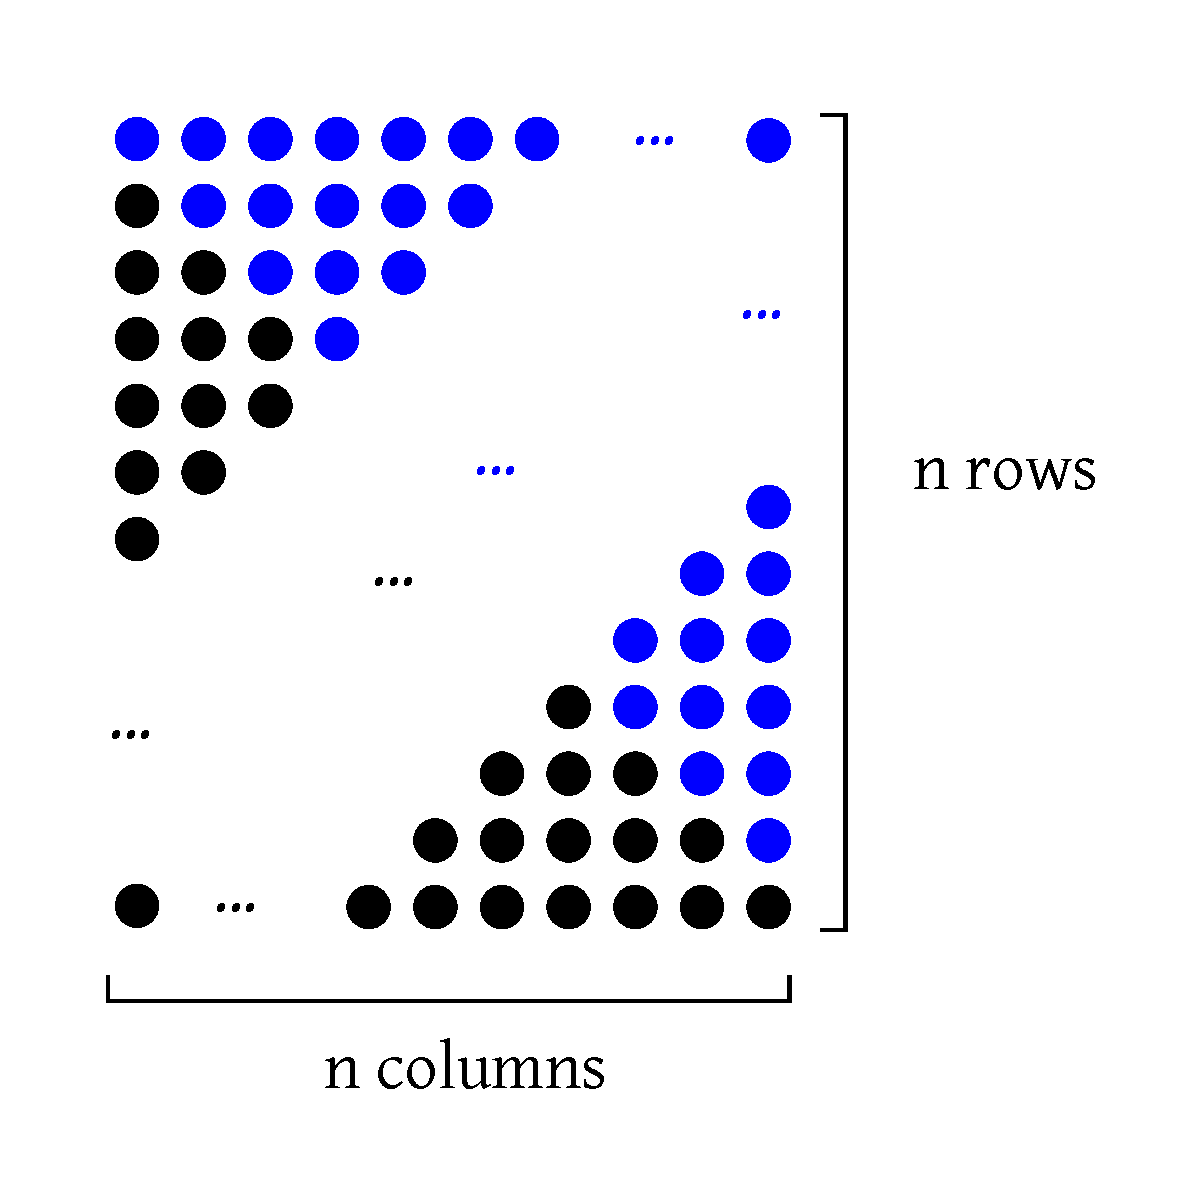
\includegraphics[width=200px]{img/triangular_number.pdf}
    \caption{Illustration of the triangular number (illustrative proof)}
  \end{center}
\end{figure}

\meta{lecture}{21st of October 2015}{Ring Wolfgang}

\begin{itemize}
  \item Let $X$ be a set. $M = \set{x \in X: P(x)}$.
  \item $\mathbb N = \set{0,1,2,3,4, \dots}$ \dots \enquote{enumerating set representation}
  \item $M = \setdef{x \in X}{P(x)}$, $N = \setdef{x \in X}{Q(x)}$
  \item $M \cup N = \setdef{x \in X}{P(x) \lor Q(x)}$
  \item Let $X$ be a set. $A_0 \subseteq X$, $A_1 \subseteq X$, $A_2 \subseteq X$, etc
  \item $\forall n \in \mathbb N: A_n \subseteq X$
  \item $A_0 \cup A_1 \cup A_2 \cup \dots = \bigcup_{n=1}^\infty A_{n} = \setdef{x \in X}{(x \in A_0) \lor (x \in A_1) \lor \dots} = \setdef{x \in X}{\exists n \in \mathbb N: x \in A_n}$
  \item $A_0 \cap A_1 \cap A_2 \cap \dots = \bigcap_{n=1}^\infty A_n = \setdef{x \in X}{\forall n \in \mathbb N: x \in A_n}$
\end{itemize}

\subsection{Cartesian product}
\index[English]{Cartesian product}
\index[German]{\foreignlanguage{ngerman}{Kartesisches Produkt}}
\begin{defi}
  Let $A$ and $B$ sets. The \emph{cartesian product of $A$ and $B$} is given as:
  \[ A \times B = \setdef{(x, y)}{x \in A, y \in B} \]
  This operation is not commutative!
\end{defi}

\begin{defi}
  We denote $\mathbb R \times \mathbb R = \mathbb R^2$.
\end{defi}

\begin{ex}
  \begin{align*}
    A &= \set{a, b, c, d, e, f, g, h} \\
    B &= \set{1, 2, 3, 4, 5, 6, 7, 8} \\
    A \times B &= \set{(a, 1), (a, 2), (a, 3), \dots, (a, 8), (b, 1), (b, 2), \dots}
  \end{align*}
\end{ex}

\begin{ex}
  \[ \mathbb R \times \mathbb R = \setdef{(x, y)}{x, y \in \mathbb R} \]
  e.g. $(1, \frac98) \in \mathbb R \times \mathbb R$.
\end{ex}

\begin{defi}
  Let $A_1, A_2, \dots, A_n$ be sets.
  \[ A_n = A_1 \times A_2 \times \dots \times A_n = \setdef{(a_1, a_2, \dots, a_n)}{a_i \in A_i \text{ for } i = 1, 2, \dots, n} \]
  instead of $\underbrace{A \times A \times \dots \times A}_{n \text{ times}} = A^n$.
\end{defi}

\subsection{Power set}
\index[English]{power set}
\index[German]{\foreignlanguage{ngerman}{Potenzmenge}}
\begin{defi}
  Let $X$ be a set. Then $\mathcal P(X)$ is the \emph{power set} of $x$.
  \[ \mathcal P(X) = \setdef{A}{A \subseteq X} \]
\end{defi}

\section{Mappings and functions}
\index[English]{mapping}
\index[German]{\foreignlanguage{ngerman}{Abbildung}}
\index[English]{domain}
\index[German]{\foreignlanguage{ngerman}{Definitionsmenge}}
\index[English]{co-domain}
\index[German]{\foreignlanguage{ngerman}{Zielmenge}}
\begin{defi}
  Let $A$ and $B$ be sets.
  A \emph{mapping} $f$ from $A$ to $B$ (denoted $f: A \rightarrow B$) is an assignment,
  such that for every $x \in A$ one $y \in B$ is assigned. We denote the corresponding
  $y \in B$ for some $x \in A$ with $y = f(x)$.
  $A$ is called \emph{domain}, $B$ is called \emph{co-domain}.
\end{defi}

\begin{defi}[Alternative definition of mappings]
  A mapping $f$ is a subset of $A \times B$ which fulfills the following properties:
  \begin{itemize}
    \item $\forall x \in A: \left(\exists y \in B: (x, y) \in f\right)$
    \item $\forall x \in A \land (y_1, y_2 \in B): \left[(x_1,y_1) \in f \land (x_1, y_2) \in f\right] \implies y_1 = y_2$
  \end{itemize}
  Notation:
  \[ (x, y) \not\in f \Leftrightarrow y = f(x) \]
  \[ \setdef{(x, f(x)) \in}{x \in A} \Rightarrow \text{graph from f} \]
\end{defi}

\index[English]{Injective function}
\index[German]{\foreignlanguage{ngerman}{Injektive Funktion}}
\index[English]{Surjective function}
\index[German]{\foreignlanguage{ngerman}{Surjektive Funktion}}
\index[English]{Bijective function}
\index[German]{\foreignlanguage{ngerman}{Bijektive Funktion}}
\index[English]{Image}
\index[German]{\foreignlanguage{ngerman}{Bildmenge}}
\index[English]{Preimage}
\index[German]{\foreignlanguage{ngerman}{Urbildmenge}}
\begin{defi}
  Let $f: A \rightarrow B$ be a mapping.
  \begin{itemize}
    \item
      The mapping $f$ is called \emph{surjective},
      if $\forall y \in B: \exists x \in A: y = f(x)$.
    \item
      The mapping $f$ is called \emph{injective}, if
      \[ \forall x_1, x_2 \in A: (f(x_1) = f(x_2) \Rightarrow x_1 = x_2). \]
    \item
      Let $B' \subseteq B$. Then we denote $f^{-1}(B') = \setdef{x \in A}{f(x) \in B'}$ as the \emph{preimage of $f$}.

      Attention! The preimage distinguishes itself from the domain (it is a subset)
      and the inverse function $f^{-1}$ (a function must not be invertible to have a preimage)!
    \item
      Let $A' \subseteq A$. Then we call $f(A') = \setdef{f(x)}{x \in A} \subseteq B$ the \emph{image of $A'$} under $f$.

      Special case: $A' = A$, then $f(A) \subseteq B$ is the image of $A$ under $f$.

      Let $f: A \rightarrow B$ be a mapping. We define $f: A \rightarrow f(A) \subseteq B$ with
      $\tilde f(x) = f(x)$ for all $x \in A$. The mapping $\tilde f$ is surjective $\forall y \in f(A)$ there exists one $x \in A$ such that $y = f(x)$.
    \item
      A mapping is called \emph{bijective}
      iff the mapping is surjective and injective.
  \end{itemize}
\end{defi}

\subsection{Bernoulli's inequality}
%
\index[English]{Bernoulli inequality}
\index[German]{\foreignlanguage{ngerman}{Bernoullis Ungleichung}}
\begin{defi}[Bernoulli's inequality]
  Let $x \in \mathbb R$ with $x > -1$ and $x \neq 0$.
  Let $n \in \mathbb N$ with $n > 1$. Then it holds that
  \[ (1 + x)^n > 1 + nx \]
\end{defi}
\begin{proof}
  Proof by complete induction.
  \begin{description}
    \item[Induction base $\mathbf{n = 2}$]
      \[ (1 + x)^2 = 1 + 2x + x^2 > 1 + 2x \quad\checkmark \]
      because $x^2 > 0$ for $x \neq 0$.
    \item[Induction step $\mathbf{n \rightarrow n+1}$] \hfill{} \\
      Assume $(1+x)^2 > 1 + n$, then $x > -1$ and $x \neq 0$.
      \[ (1 + x)^{n+1} = (1 + x)^n \cdot \underbrace{(1 + x)}_{>0} > (1+nx) \cdot (1 + x) \]
      \[ = (1 + nx + x + nx^2) = (1 + (n+1)\cdot x + \underbrace{nx^2}_{>0}) > 1 + (n + 1) \cdot x \]
  \end{description}
\end{proof}

\index[English]{Bijective function}
\index[German]{\foreignlanguage{ngerman}{Bijektive Funktion}}
\index[English]{Composition of functions}
\index[German]{\foreignlanguage{ngerman}{Verknüpfung von Funktionen}}
\index[English]{Identity function}
\index[German]{\foreignlanguage{ngerman}{Identitätsfunktion}}
\index[English]{Inverse function}
\index[German]{\foreignlanguage{ngerman}{Inverse Funktion}}
% TODO: extend
Back to sets and functions (notes missing):
\begin{itemize}
  \item injective, surjective, bijective function
  \item composition of functions: Let $f: X \rightarrow Y$ and $g: Y \rightarrow Z$. $g \circ f: X \rightarrow Z$ is defined as $g(f(x))$ (\enquote{g after f}).
  \item Let $f$ and $g$ be mappings. If $f$ and $g$ are injective, $f \circ g$ is injective. If $f$ and $g$ are surjective, $f \circ g$ is surjective. If $f$ and $g$ are bijective, $f \circ g$ is bijective.
  \item Identity function, $f \circ \operatorname{id} = \operatorname{id} \circ f = f$
  \item properties of an inverse function, $f \circ f^{-1}: X \rightarrow X$, $f^{-1} \circ f: X \rightarrow X$
\end{itemize}

\section{About sums of integers}
\meta{lecture}{21st of Oct 2015}{Wolfgang Ring}

\begin{defi}
  The summation notation is defined as,
  \[ \sum_{k=h}^{l} a_k \]
  Iteration over all values from $l$ to $h$ (inclusive) and evaluation of
  the enclosed expression with $k$ as iteration value. The resulting terms
  are added up and the sum gives the result of the summation expression.
\end{defi}

Laws:
\begin{align}
    \sum_{k=l}^{h} a_k &= \sum_{i=l}^h a_i \\
    \sum_{k=l}^{h} (a_k + b_k)
        &= \left(\sum_{k=l}^h a_k\right) + \left(\sum_{k=l}^h b_k\right) \\
    \sum_{k=0}^{h} a_k
        &= a_0 + \sum_{k=1}^{h} a_k
        & \text{\enquote{Extraction of the initial value}} \\
    \sum_{k=0}^{h} a_k
        &= a_{h} + \sum_{k=0}^{h-1} a_k
        & \text{\enquote{Extraction of the final value}} \\
    \sum_{k=u+n}^{h+n} a_k
        &= \sum_{k=u}^{h} a_{k+n}
        & \text{\enquote{index shifting}} \\
    \sum_{k=l}^h \lambda \cdot a_k
        &= \lambda \cdot \sum_{k=l}^h a_k
        & \text{\enquote{extraction of a constant $\lambda$}} \\
    \sum_{k=0}^n n
        &= \frac{n (n+1)}{2}
        & \text{\enquote{triangular sum}}
\end{align}

We consider $S_n = \set{(a_1, a_2, \ldots, a_n): a_i \in M_n \forall i = 1, \ldots, n
\text{ with } a_i \neq a_j} \subseteq M_n \times M_n \times \dots \times M_n$.
$S_n$ is the set of all arrangements of the numbers $1, \ldots, n$.

Example: $\set{(1,2,3), (1, 3, 2), (2, 1, 3), (2, 3, 1), (3, 1, 2), (3, 2, 1)}$

\subsection{Factorials}
%
\begin{theorem}
  It holds that $\card{S_n} = n!$ for all $n \in \mathbb{N}$
\end{theorem}
\begin{proof}
  Proof by induction over $n$.
  \begin{description}
    \item[Induction base]
      $n=1$:
        $M_1 = \set{1}, S_1 = \set{(1)} \Rightarrow \card{S_1} = 1 = 1! \done$
    \item[Induction step]
      $n\rightarrow n+1$:
        \[
          S_{n+1} = \set{(a_1, a_2, \ldots, a_n) :
              a_i \in M_{n+1} \forall i \in M_{n+1},
              a_i \neq a_j \text{ for } i \neq j}
        \]
        For $l \in M_{n+1}$: \[
          W_l = \set{(a_1, \ldots, a_{n+1}) \in S_{n+1}: a_l = n+1}
        \]
        It holds that $W_l \cap W_j = \emptyset$ for $l \neq j$
        and $S_{n+1} = W_i \cup W_l \cup W_j \cup \ldots \cup W_{n+1}$.
        Then it holds that $\card{S_{n+1}} = \card{W_1} + \card{W_2} + \ldots + \card{W_{n+1}} = \sum_{l=1}^{n+1} \card{W_l}$

        \begin{theorem}
          Claim: For every $l \in M_{n+1}$ it holds that $\card{W_l} = \card{S_n} = n!$.
        \end{theorem}
        \begin{proof}
          We build a bijective map $\phi_l: W_l \rightarrow S_n$.
          \[
              W_l = \set{(a_1, a_2, \ldots, a_{l-1}, n+1, a_{l+1}, \ldots, a_{n+1}}
          \]\[
                  :a_i \in M_n, \forall i \neq l, a_i \neq a_j \forall i \neq j
          \] \[
              \phi\left((a_1, a_2, \ldots, a_{l-1}, n+1, a_{l+1}, \ldots, a_{n+1})\right)
          \] \[
                  = (a_1, a_2, \ldots, a_{l-1}, a_{l+1}, \ldots, a_{n+1}) \in S_n
          \]

          $S_n$ is surjective.
          Let $(b_1, \ldots, b_n) \in S_n$, then it holds that $(b_1, \ldots, b_{l-1}, n+1, b_l, \ldots, b_n) \in W_l$
          \[ \phi_l((b_1, \ldots, b_{l-1}, n+1, b_l, \ldots, b_n)) = (b_1, \ldots, b_n) \]

          $S_n$ is injective.
          \[
              \phi_l((a_1, \ldots, a_{l-1}, n+1, a_{l+1}, \ldots, a_{n+1}))
          \] \[
                  = \phi_l((a_1, \ldots, a_{l-1}, n+1, a_{l+1}, \dots, a_{n+1}))
          \] \[
               \Rightarrow
               (a_1, \ldots, a_{l-1}, a_{l+1}, \ldots, a_{n+1}) =
               (a_1, \ldots, a_{l-1}, a_{l+1}, \ldots, a_{n+1})
          \]
          $\phi$ is bijective.
        \end{proof}

        Therefore $\card{W_l} = \card{S_n} = n!$.
        Therefore $\card{S_{n+1}} = \sum_{l=1}^{n+1} \card{S_n} = \sum_{l=1}^{n+1} n! = (n + 1) n! = (n + 1)!$
  \end{description}
\end{proof}

\begin{rem}
  Let $f: M_n \rightarrow M_n$. $f$ is represented as
  \[  (1, 2, 3, 4, \ldots, n-1, n) \rightarrow (f(1), f(2), f(3), f(4), \ldots, f(n-1), f(n))  \]
  Therefore $(f(1), f(2), \ldots, f(n)) \in S_n$. Analogously every $(a_1, \ldots, a_n) \in S_n$
  defined by $f(k) = a_k$ for $k=1,\ldots,n$ is a bijective mapping $f: M_n \rightarrow M_n$.
  Therefore we set $S_n = \set{f: M_n \rightarrow M_n: f \text{ is bijective}}$.
  $S_n$ is called symmetric group of $n$ elements.
\end{rem}

\subsection{Binomial coefficients}
\begin{defi}
  Let $n \in \mathbb{N}$, $k \in \mathbb{N}$ with $k \leq n$.
  We define \begin{align*}
    \binom{n}{k} &= \frac{n!}{k! (n-k)!}   & \text{\enquote{binomial coefficient $n$ choose $k$}}
  \end{align*}
\end{defi}

It holds that
\begin{align*}
  \binom{n}{k} &= \frac{1\cdot 2\cdot 3\cdot \ldots \cdot n}{(1 \cdot 2 \cdot \ldots \cdot k) (1 \cdot 2 \cdot 3 \cdot \ldots \cdot (n-k))} \\
               &= \frac{n (n-1) \cdot \ldots \cdot (k+1)}{(1 \cdot 2 \cdot 3 \cdot \ldots \cdot (n-k))}
\end{align*}

Factorial laws:
\begin{align*}
  \binom 10 &= \frac{n!}{0! (n-0)!} = 1 \qquad \forall n \in \mathbb{N} \\
  \binom nn &= \frac{n!}{n! (n - n)!} = \frac{n!}{n! \cdot 1} = 1 \\
  \binom{n}{n-k} &= \frac{n!}{(n-k!)(n - n + k)!} = \frac{n!}{k! (n-k)!} = \binom nk & \text{\enquote{symmetrical}}
\end{align*}

A recursive definition is given by
\begin{align*}
    \binom nk &= \binom{n-1}{k-1} + \binom{n-1}{k}
    & n \geq 1, 1 \leq k \leq n-1
\end{align*}

\begin{proof}
  \begin{align*}
      \binom{n-1}{k-1} + \binom{n-1}{k}
          &= \frac{(n-1)!}{(n-1)! (n-1 - (k-1))!} \\
          &= \frac{(n-1)!}{k! (n-1-k)!} \\
      &= \frac{(n-1)!}{(k-1)! (n-k)!} + \binom{(n-1)!}{k! (n-1-k)!} \\
      &= \frac{k \cdot (n-1)! + (n-k)(n-1)!}{k! (n-k)!} \\
      &= \frac{n (n-1)!}{k!(n-1)!} = \frac{n!}{k! (n-k)!} \\
      &= \binom nk
  \end{align*}
\end{proof}

\subsection{Arrangement in Pascal's triangle}
\begin{figure}[!h]
  \begin{center}
    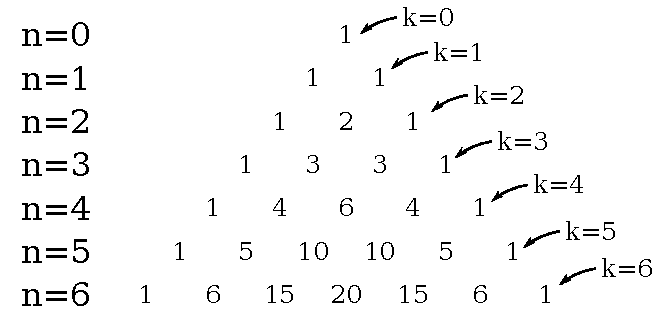
\includegraphics{img/pascals_triangle.pdf}
    \caption{
      Pascal's triangle describes binomial coefficients.
      For every element of the triangle it holds that,
      it is adding up the two numbers above a number.
      The margins are defined by $1$. For example $5$ is given by ${5 \choose 4}$.
    }
  \end{center}
\end{figure}

\begin{theorem}
  Let $T_n^k = \set{A \subseteq M_n: \card{A} = k}$.
  Then it holds that $\card{T_n^k} = \binom nk$.

  Example: $T_3^2 = \set{\set{1, 2}, \set{1, 3}, \set{2, 3}}$.

  $\card{T_3^2} = \binom 32 = \frac{3!}{2! 1!} = \frac 62 = 3$
\end{theorem}

\begin{proof}
  Let $n$ be fixed. Induction for $k$.
  \begin{description}
    \item[Induction base] $k=0$
      \begin{align*}
        T_n^0        &= \set{\emptyset} \\
        \card{T_n^0} &= 1 = \binom n0
      \end{align*}
    \item[Induction step] $k\rightarrow k+1$
      \begin{align*}
        T_n^k &= \underbrace{\set{\set{a_1, \ldots, a_k}: a_1 \in M_n, (i = 1, \ldots, k), a_i \neq a_j \text{ for } i \neq j}}_{A_1} \\
              &\cup \underbrace{\set{\set{a_1, \ldots, a_{k-1}} \cup [n] \in M_{n-1}}}_{A_2} \\
        \card{T_N^k} &= \card{A_1} + \card{A_2}
      \end{align*}
  \end{description}
\end{proof}

\meta{lecture}{28th of October 2015}{Ring Wolfgang}

Let $A, B$ be sets and define
\[ A \setminus B = \set{x: x \in A \land x \not\in B} \]
Then the domain of $A \setminus B$ is \enquote{A without B}.

\begin{theorem}
  \[ T_n^x = \set{x \subseteq M_x: \card{X} = x} \]
  Let $k \in \mathbb{N}$ and $0 \leq k \leq 1$.
  \[ \card{T_n^x} = \binom{1}{k} \]
  There are exactly $\binom{n}{k}$ k-ary subsets of $M_n$.
\end{theorem}

\begin{proof}
  \[
      M_0 = \emptyset \qquad
      T_0^0 = \set{\emptyset} \qquad
      \card{T_n^0} = 1 = \binom{0}{n}
  \]
  Proof by complete induction over $n$ of the following statement:
  \[
    \forall n \in \mathbb{N}: \forall k \in \mathbb{N} \text{ with } 0 \leq k \leq n:
    \card{T_n^k} = \binom{n}{k}
  \]
  \begin{description}
    \item[Induction base]
      $n = 0$ is fine.
      For $n = 1$ there are two cases: $k = 0$ or $k = 1$.
      \[ M_1 = \set{1} \]
      \[ T_1^0 = \set{\emptyset} \qquad \card{T_1^0} = 1 = \binom{1}{0} \]
      \[ T_1^1 = \set{\set{1}} \qquad \card{T_1^1} = 1 = \binom{1}{1} \]
      Is also fine.
    \item[Induction step]
      The hypothesis is our assumption:
      \[ \forall 0 \leq k \leq 1: \card{T_n^k} = \binom{n}{k} \]

      Consider $M_{n+1}$. Special case $k = 0$:
      \[ T_{n+1}^0 = \set{\emptyset} \qquad \card{T_{n+1}^0 = 1 = \binom{n+1}{0}} \]

      Special case $k = n + 1$:
      \[ T_n^{} = \set{M_{n+1}} \qquad \card{T_N{n+1}^{n+1}} = 1 = \binom{n+1}{n+1} \]

      Let $1 \leq k \leq n$.
      \[ T_{n+1}^x TODO \]

      Union is disjoint $\Rightarrow \card{T_{n+1}^k} = \card{R_{n+1}^k} + \card{S_{n+1}^k}$

      \[ R_{n+1}^k = \set{A \subseteq M_n: \card{A} = k} = T_n^k \]
      \[ \card{R_{n+1}^k} = \card{T_n^k} = \binom{n}{k} \]
      by induction hypothesis.
      \[ S_{n+1}^k = \set{A \subseteq M_{n+1}: A = A' \cup \set{n+1}: A' \subseteq M_n: \card{A'} = k - 1} \]
      We prove $\card{S_{n+1}^k} = \card{T_n^{k-1}}$.
      \[ f: S_{n+1}^k \rightarrow T_n^{k-1} \]
      \[ f(A) = f(A' \cup \set{n+1}) = A' \]

      $f$ is bijective.
      $f$ is surjective: Let $A' \in T_n^k$ define $A = A' \cup \set{n+1} \in S_{n+1}^n$ and $f(A) = A'$.
      $f$ is injective: Let $f(A) = f(B)$ and $A = A' \cup \set{n+1} \in S_{n+1}^k$.

      $B = B' \cup \set{n+1} \in S_{n+1}^k$. $A', B' \in T_n^{k-1}$.

      \[ f(A) = f(B) \Rightarrow A' = B' \Rightarrow A' \cup \set{n+1} = B' \cup \set{n+1} \Rightarrow A = B \]
      \[ \card{S_{n+1}^k} = \card{T_n^{k-1}} \stackrel{\text{ind. hypo.}}{=} \binom{n}{k-1} \]
      Therefore $\card{T_{n+1}^k} = \binom nn = \binom n{k-1} = \binom{n+1}{k}$.
      The last equation follows from the recursive definition of binomial coefficients.
  \end{description}
\end{proof}

\subsection{Binomial theorem}
\begin{theorem}[Binomial theorem]
  Let $a, b \in \mathbb{R}$ (or $a, b \in \mathbb{C}$). Then it holds that
  \[ (a + b)^n = \sum_{k=0}^n \binom{n}{k} a^k b^{n-k} \]
\end{theorem}

\begin{proof}
  \begin{enumerate}
    \item
      Proof by induction over $n$.
      \begin{description}
        \item[Induction step] $n=0$: $(a + b)^0 = 1$
          \[ \sum_{k=0}^0 \binom{0}{k} a^k b^{0-k} = \binom{0}{0} a^0 b^0 = 1 \]
        \item[Induction step] $n \rightarrow n + 1$
          \[
            (a + b)^{n+1} = (a + b)^n \cdot (a + b)
            = \left(\sum_{k=0}^n \binom nk a^k b^{n-k}\right) (a + b)
          \] \[
            = \sum_{k=0}^n \binom nk a^{k+1} b^{n-k} + \sum_{k=0}^n \binom nk a^k b^{n-k+1}
          \] \[
            = \underbrace{\sum_{n=0}^{n-1} \binom nk a^{k+1} b^{n-k}}_{\substack{\text{index shift} \\ h + 1 = j, h =0 \\ \Rightarrow j=1, h = j-1, h=n-1 \\ \Rightarrow j = n}} +
              \underbrace{\binom nk a^{n+1} \cdot b^0}_{a^{n-1}}
          \] \[
            + \sum_{k=1}^n \binom nk a^k b^{n+1-k} +
              \binom n0 a^0 b^{n+1}
          \] \[
            \sum_{j=1}^n \binom{n}{j-1} a^j b^{n-(j-1)}
            + \sum_{k=1}^n \binom nk a^k b^{n+1-k}
          \] \[
            + \binom{n+1}{n+1} a^{n+1}
            + \binom{n+1}{0} b^{n+1}
          \]
          Renaming $j$ to $k$:
          \[
            = \sum_{k=1}^n \underbrace{\left[\binom{n}{k-1} + \binom nk\right]}_{\binom{n+1}{k} \text{ by recursive definition}} a^k b^{n+1-k}
          \] \[
            + \binom{n+1}{n+1} a^{n+1} b^0
            + \binom{n+1}{0} a^0 b^{n+1}
          \] \[
            = \sum_{k=0}^{n+1} \binom{n+1}{k} a^k b^{n+1-k}
          \]
          Therefore the binomial theorem holds for $n+1$.
      \end{description}
  \end{enumerate}
\end{proof}

\meta{lecture}{29th of October 2015}{Ring Wolfgang}

\[ \forall a, b \in \mathbb{R}, n \in \mathbb{N}: (a + b)^n = \sum_{k=1}^n \binom{n}{k} a^k b^{n-k}  \]
\begin{description}
  \item[Induction base] $n = 0, n = 1$ follows immediately
  \item[Induction step]
    \[ (a + b)^n = \underbrace{(a + b)(a + b)(a + b)(a + b)\dots(a + b)}_{n \text{ times}} \]
    When multiplying the products $a^n b^{n-k}$ are created ($0 \leq k \leq n$).
    $a^n b^{n-k}$ are created iff $a$ is the factor resulting from $k$ parenthesis groups and
    $b$ originates from the remaining $(n-k)$ groups.
    There are exactly $\binom{n}{k}$ possibilities to select from $n$ groups.
    $a^k b^{n-k}$ occurs $\binom nk$ times.
    Therefore
    \[ (a + b)^n = \sum_{k=0}^n \binom nk a^k b^{n-k} \]
    This is a rather informal proof, but suffices at this point.
\end{description}

\section{Arithmetics of numbers}
%
We consider two fundamental arithmetic operators and determine fundamental properties.

\begin{defi}
  Let $K$ be a set where two arithmetic operators are defined:
  Therefore $\forall a,b \in K$ let $a + b \in K$ and $a \cdot b \in K$.

  We require the following properties:
  \begin{itemize}
    \item[\textbf{A1}] $\forall a,b \in K: a + b = b + a$
    \item[\textbf{A2}] $\forall a,b,c \in K: (a + b) + c = a + (b + c)$
    \item[\textbf{A3}] $\exists 0 \in K \forall a \in K: a + 0 = a$
    \item[\textbf{A4}] $\forall a \in K \exists \tilde{a}: a + \tilde{a} = 0$
  \end{itemize}
  Then $(K, +)$ is a commutative group (\enquote{abelian group}).
  In general we denote $\tilde{a}$ as $-a$.
  We define $a - b = a + (-b)$ (\enquote{subtraction}).

  \begin{itemize}
    \item[\textbf{M1}] $\forall a,b \in K: a \cdot b = b \cdot a$
    \item[\textbf{M2}] $\forall a,b,c \in K: a \cdot (b \cdot c) = (a \cdot b) \cdot c$
    \item[\textbf{M3}] $\exists 1 \in K: a \cdot 1 = a \forall a \in K$ (neutral element)
    \item[\textbf{M4}] $\forall a \in K \setminus \set{0} \exists \hat a: \hat a \cdot a = 1$
  \end{itemize}
  In general we denote $\hat a$ as $a^{-1}$.

  We set $\frac ab = a \cdot b^{-1}$.
  \[ \frac{1}{b} = 1 \cdot b^{-1} \text{ for } b \neq 0 \]
\end{defi}

\begin{defi}[Composition]
  Compatibility of $+$ and $\cdot$:
  \begin{itemize}
    \item[\textbf{D}] $\forall a,b,c \in K: a \cdot (b + c) = a \cdot b + a \cdot c$
  \end{itemize}
  Under these conditions $K$ is called a \emph{field}.
\end{defi}

\begin{ex}
  Examples for fields: $\mathbb{Q}, \mathbb{R}, \mathbb{C}$.

  In every field it holds that
  \begin{itemize}
    \item the inverse element of $a$ is unique ($\tilde a$ is unique).
      Let $-a$ be the inverse element of $a$ and $a + b = 0 \Rightarrow b = -a$
      \begin{proof}
        TODO
        \[ (a + (-a)) + (b + 0) = a + b =  \]
      \end{proof}
    \item $0 \cdot a = 0$
      \begin{proof}
        \[ 0 = 0 + 0 \]
        follows from \textbf{D}.
        \[ 0 \cdot a = (0 + 0) \cdot a = 0 \cdot a + 0 \cdot a \]
        \[ 0 \cdot a + (-0 \cdot a) = 0 \cdot a + \left[0 \cdot a + (-0 \cdot a)\right] \]
        \[ 0 = 0 \cdot a \]
      \end{proof}
    \item $-a = (-1) \cdot a$
      \begin{proof}
        \begin{align*}
          a + (-1) \cdot a = (1 + (-1)) a = 0 \\
          a + (-1) \cdot a = 0 \\
          -a = (-1) \cdot a \\
        \end{align*}
      \end{proof}
  \end{itemize}
\end{ex}

\subsection{Integers and the field of rational numbers $\mathbb{Q}$}
%
For $\mathbb{N}$, \textbf{A1}, \textbf{A2} and \textbf{A3}.
If $n \geq m$, then also $n - m \in \mathbb{N}$.
$n-m = k \in \mathbb{N}$ is defined in such a way that $n = m + k$.

\begin{cor}
  Extension:
  \[ \mathbb{Z} = \set{0, 1, -1, 2, -2, 3, \ldots} = \mathbb{N}_+ \cup \set{0} \cup \set{-n: n \in \mathbb N_0} \]
  We define $-0 \coloneqq 0$ and $\forall n \in \mathbb{N}_+$ let $n + (-n) \coloneqq 0$.

  Therefore for every $z \in \mathbb{Z}$ exists some $\tilde z$ such that $z + \tilde z = 0$.
  \begin{itemize}
    \item $z \in \mathbb{Z}_+ \Rightarrow \tilde z = -z$
    \item $z = 0 \Rightarrow \tilde z = 0$
    \item $z = -n$ for $n \in \mathbb{N}_+$
    \item $\tilde z = n$
  \end{itemize}
  \[ \forall z \in \mathbb{Z} \exists \tilde z \in \mathbb{Z}: z + \tilde z = 0 \]
  In general we denote $\tilde z = (-z)$.
  Also $-(-z) = z$.

  For $z,w \in \mathbb{Z}$:
  \[
    z + w =
    \begin{cases}
      z + w       & z,w \in \mathbb{N} \\
      (-z) + (-w) & -z, -w \in \mathbb{N} \\
      z - (-w)    & z, -w \in \mathbb{N} \text{ and } z > (-w) \\
      -((-w) - z) & z, -w \in \mathbb{N} \text{ and } (-w) > z
    \end{cases}
  \] \[
    z\cdot w =
    \begin{cases}
      z \cdot w       & z,w \in \mathbb{N} \\
      (-z)(-w)        & -z, -w \in \mathbb{N} \\
      -((-z) \cdot w) & -z \in \mathbb{N}, w \in \mathbb{N}
    \end{cases}
  \]

  In $\mathbb{Z}$ the properties \textbf{A1}, \textbf{A2}, \textbf{A3}, \textbf{A4},
  \textbf{M1}, \textbf{M2}, \textbf{M3} and \textbf{D} hold.
\end{cor}

\begin{defi}
  \[ \mathbb{Q} = \set{\frac mn: m,n \in \mathbb{Z}, n \neq 0} \]
  where $\frac mn = \frac{m'}{n'} \Leftrightarrow m \cdot n' = n \cdot m'$.
  $\mathbb{Q}$ is called the set of rational numbers.

  We define
  \[ \frac mn + \frac kl \coloneqq \frac{ml + nk}{nl} \]
  \[ \frac mn \cdot \frac kl = \frac{mk}{nl} \]

  Show that
  \[ \frac mn = \frac{m'}{n'} \text{ and } \frac kl = \frac{k'}{l'} \]
  \[ \Rightarrow \frac{ml + nk}{nl} = \frac{m'l' + n'k'}{n'l'} \]
  \[ \Rightarrow (ml + nk)(n' l') = (m' l' + n' k') \]
  \[ \Leftrightarrow mn' \cdot ll' + nn' \cdot kl = m'n \cdot ll' + nn' \cdot k' l \]
  Analogously for $\frac mn \cdot \frac kl$.

  \textbf{A1}--\textbf{A4}, \textbf{M1}--\textbf{M4} and \textbf{D} hold for $\mathbb{Q}$.

  For $z \in \mathbb{Z}$ we set $z = \frac z1$.
  Therefore it holds that $\mathbb{Z} \subseteq \mathbb{Q}$.
  $0 = \frac 01$ and $\frac mn + 0 = \frac mn + \frac 01 = \frac{m\cdot 1 + n\cdot 0}{n\cdot 1} = \frac{m \cdot 1}{n\cdot 1} = \frac mn$.
  $0$ is neutral in regards of addition in $\mathbb{Q}$.

  Inverse element in regards of addition:
  \[ \frac mn + \frac{-m}n = \frac{mn + (-m)n}{n^2} = \frac{(m + (-m)) n}{n \cdot n} = \frac{0n}{n^2} = \frac 01 \]
  because $0 \cdot 1 = 0 \cdot n^2$.

  Concerning multiplication:
  \[ 1 = \frac 11 \qquad \frac mn \cdot \frac 11 = \frac{m\cdot 1}{n\cdot 1} = \frac mn \]
  $1$ is a neutral element in regards of multiplication in $\mathbb{Q}$.

  Let $\frac mn \in \mathbb{Q} \setminus \set{0} \Rightarrow m \neq 0 \Rightarrow \frac nm \in \mathbb{Q}$ and $\frac mn \frac nm = \frac{mn}{mn} = \frac 11$. TODO: verify
  because $m \cdot n \cdot 1 = 1\cdot m \cdot n$.
\end{defi}

\begin{cor}
  \[ \forall \frac mn \in \mathbb{Q}: -\frac mn = \frac{-m}{n} \]
  \[ \forall \frac mn \in \mathbb{Q} \setminus \set{0}: \left(\frac mn\right)^{-1} = \left(\frac nm\right) \]
  Therefore $\mathbb{Q}$ is a field.
\end{cor}

\meta{lecture}{30th of October 2015}{Ring Wolfgang}

Literature:
\begin{itemize}
  \item Eblinghaus et al., \enquote{Zahlen}, Springer Verlag
  \item E. Landau: \enquote{Grundlagen der Analysis}, uses Peano axioms to build calculus
\end{itemize}

\subsection{Ordered fields}
\begin{defi}
  Let $K$ be a field. We assume that $K$ is taken from two sets: $K = K_+ \cup \set{0} \cup K_-$
  with $0 \not\in K_+, 0 \not\in K_-$. It holds that
  \begin{itemize}
    \item $\forall a \in K$ it holds that either $a \in K_+$ or $a = 0$ or $a \in K_+$ \\
          $a \in K_+ \Leftrightarrow -a \in K_-$
    \item $\forall a, b \in K_+$: $a + b \in K \land a\cdot b \in K$
  \end{itemize}
  If those properties are satisfied, such a field is called an \emph{ordered field}.
  Instead of $a \in K_+$ we write $a > 0$ (namely \enquote{positive numbers})
  and $a < 0$ for $a \in K_-$ correspondingly (namely \enquote{negative numbers}).

  For arbitrary $a, b \in K$ we define
  \[ a > b \Leftrightarrow a - b > 0 \]
  It holds that $a > b \Leftrightarrow b < a$.
  \[ a \geq b \Leftrightarrow a > b \lor a = b \]
\end{defi}

\begin{lemma}
  Let $K$ be an ordered field. Then it holds that
  \begin{enumerate}
    \item $a \in K_+ \land b \in K_- \Rightarrow a \cdot b \in K_-$ \\
          $a \in K_- \land b \in K_- \Rightarrow a \cdot b \in K_+$
    \item $\forall a, b \in K$ one of the following relations hold:
          \[ a > b \lor a = b \lor a < b \]
          Therefore $<$ defines a total order on $K$.
    \item $\forall a, b, c \in K: \left[(a < b) \land (b < c) \implies a < c\right]$ \\
          Therefore $<$ is transitive.
    \item If $a > b > 0$ then $\frac1a < \frac1b$
          If $a > 0$ holds, then also $a^{-1} = \frac1a > 0$.
    \item $\forall a, b, c \in K: a < b \implies a + c < b + c$
    \item $\forall a, b \in K: \forall c > 0: \left[a > b \implies ac > bc\right]$ \\
          $\forall a, b \in K: \forall c < 0: \left[a > b \implies ac < bc\right]$
    \item $\forall a \in K \setminus \set{0}: a^2 = a \cdot a > 0$
  \end{enumerate}
\end{lemma}

\begin{proof}
  \begin{enumerate}
    \item We know from the practicals: $\forall a,b \in K: (-a)(-b) = ab$
      \[ (-a) b = -(ab) \]
      Let $a \in K_+, b \in K_-$, therefore $a \in K_+$, $(-b) \in K_-$,
      then it holds that $ab = (-a)(-b) = -(a(-b)) \in K_-$.
      Let $a \in K_-$ and $b \in K_-$ therefore $(-0) \in K_+ \land (-b) \in K_+
      \implies ab = (-a)(-b) \in K_+$.
    \item Let $a, b \in K$. Then one of the following properties hold:
      \[ a - b > 0 \lor a - b = 0 \lor a - b < 0 \]
      Equivalently,
      \[ a > b \lor a = b \lor a < b \]
    \item Let $a > b$ and $b > c$. Therefore $a - b > 0$ and $b - c > 0$.
      \[ \Rightarrow (a - b) + (b - c) > 0 \]
      \[ a(- b + b) - c > 0 \]
      \[ a - c > 0 \Leftrightarrow a > c \]
    \item Let $a > 0 \Rightarrow a^{-1} \neq 0$.
      Assume $\frac{1}{a} = a^{-1} < 0 \Rightarrow a^{-1} \cdot a = 1 < 0$.
      Otherwise it holds that $1 = 1 \cdot 1 = 1^2 > 0 \lightning$
    \item Let $a > b > 0$. Then it holds that
      \[
          a^{-1} b^{-1} (b - a)
          = a^{-1} b^{-1} b - a^{-1} b^{-1} a
          = -a^{-1} \cdot b^{-1}
          = \frac1a \cdot \frac1b
          \Rightarrow a^{-1} < b^{-1}
      \]
    \item $a < b$ therefore $a - b < 0 \Rightarrow a + c - c - b < 0 \Rightarrow (a + c) - (b + c) < 0$
      \[ \Leftrightarrow a + c < b + c \]
    \item Let $a > b, c > 0 \Rightarrow (a - b) > 0 \Rightarrow (a - b) \cdot c > 0 \Rightarrow ac - bc > 0
      \Rightarrow ac > bc$. For the second statement, it holds analogously:
      $a < b, c < 0 \Rightarrow (a - b) < 0 \Rightarrow (a - b) \cdot c < 0 \Rightarrow ac - bc < 0
        \Rightarrow ac < bc$
    \item $a > 0 \Rightarrow a \cdot a > 0$.
      Let $a < 0 \Rightarrow (-a) > 0$. It holds $a \cdot a = (-a)(-a) > 0$.
      Therefore the square of two numbers is always positive.
  \end{enumerate}
\end{proof}

\subsection{Remarks about some common fields}
\begin{rem}
  $\mathbb{C}$ is not an ordered ordered field.
  $\mathbb{N}$, $\mathbb{Z}$ and $\mathbb{Q}$ are ordered.
\end{rem}

\begin{rem}
  Let $q \in \mathbb{Q}$.
  \begin{itemize}
    \item[a)] Let $m,n \in \mathbb{N}_+$ such that $q = \frac mn$ then $q > 0$.
    \item[b)] Let $m,n \in \mathbb{N}_+$ such that $q = -\frac mn$ then $q < 0$.
  \end{itemize}

  We show that $\mathbb{Q} = \mathbb{Q}_+ \cup \set{0} \cup \mathbb{Q}_-$.
  Every $q \in \mathbb{Q}$ has a representation of either a) or b), but not both.
  $\mathbb{Q}_+ \cap \mathbb{Q}_- = \emptyset$.

  \[
    q \neq 0 \Rightarrow q = \begin{cases}
      \frac mn & m,n \in \mathbb{N}_+ \\
      -\frac mn & m,n \in \mathbb{N}_+ \\
      -\frac mn & m,n \in \mathbb{N}_+ \\
      \frac{-m}{-n} & m,n \in \mathbb{N}_+
    \end{cases}
  \]
  \[ q = \frac{n}{-m} = \frac{-n}{m} \]
  because $nm = (-n)(-m)$.
  \[ q = \frac{-m}{-n} = \frac mn \]
  because $(-m) \cdot n = m \cdot (-n)$.
\end{rem}

\begin{rem}
  We want to show that $\mathbb{Q}_+ \cap \mathbb{Q}_- = \emptyset$.
  Let $q \in \mathbb{Q}_+ \cap \mathbb{Q}_-$.
  \[ q = \frac mn = -\frac{m'}{n'} \qquad m,n,m',n' \in \mathbb{N}_+ \]
  \[ \Rightarrow n \cdot n' = (-m') n \]
  \[ \Rightarrow \underbrace{\underbrace{mn'}_{\in \mathbb{N}_+} + \underbrace{m' n}_{\in \mathbb{N}_+}}_{\in \mathbb{N}_+} = 0 \qquad\text{\Lightning} \]

  Furthermore $p \in \mathbb{Q}_+ \land q \in \mathbb{Q}_+$
  \[ \Rightarrow p + q \in \mathbb{Q}_+ \land pq \in \mathbb{Q}_+ \]
  \[ \Rightarrow p = \frac kl \qquad q = \frac mn \qquad k,l,m,n \in \mathbb{N}_+ \]
  \[ p + q = \frac{\overbrace{kn + ml}^{\in \mathbb{N}_+}}{nm} \in \mathbb{Q}_+ \]
  \[ pq = \frac{k}{l} \cdot \frac mn = \frac{\overbrace{km}^{\in \mathbb{N}_+}}{\underbrace{ln}_{\in \mathbb{N}_+}} \in \mathbb{Q}_+ \]
\end{rem}

\begin{figure}[!h]
  \begin{center}
    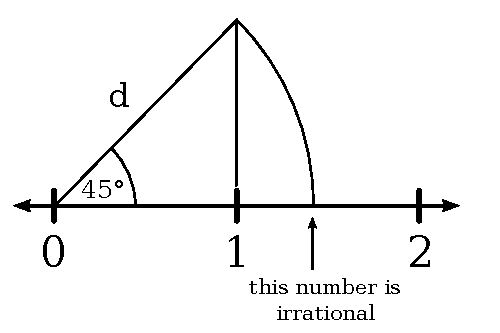
\includegraphics[width=200px]{img/irrational_number.pdf}
    \caption{Illustration of an irrational number}
  \end{center}
\end{figure}

\begin{defi}
  Let $K$ be an ordered field $a \in K$.
  The absolute value of $a$ is defined as
  \[
    \abs{a} = \begin{cases}
      a & \text{ if } a \in K_+ \\
      0 & \text{ if } a = 0 \\
      -a & \text{ if } a \in K_-
    \end{cases}
  \]
\end{defi}

\begin{rem}
  Let $K$ be an ordered field. Then it holds that
  \[ \mathbb{Q} \subseteq K \subseteq \mathbb{R} \]
  except for isomorphism.
\end{rem}

\subsection{Triangle inequality}
\begin{theorem}
  \[ \forall a, b \in K: \abs{a + b} \leq \abs{a} + \abs{b} \qquad \text{\enquote{Triangle inequality}} \]
  %\[ \abs{a \cdot b} = \abs{a} \cdot \abs{b} \]
\end{theorem}
\begin{proof}
  \begin{description}
    \item[Case 1]
      \[ a \cdot b > 0 \Rightarrow a \cdot b > 0: \abs{ab} = ab \qquad \abs{a}\cdot\abs{b} = ab \]
    \item[Case 2]
      \[ a > 0, b < 0: a \cdot b < 0: \abs{ab} = -ab \qquad \abs{a} \cdot \abs{b} = a \cdot (-b) \]
      \[ b < 0 \Rightarrow -b > 0 \Rightarrow b < -b \Rightarrow \underbrace{a + b}_{\abs{a + b}} < \underbrace{a - b}_{\abs{a} + \abs{b}} \]
    \item[Case 3]
      \[ a < 0, b < 0: a \cdot b > 0: \abs{ab} = ab \qquad \abs{a} = -a \qquad \abs{b} = -b  \]
      \[ \abs{a} \cdot \abs{b} = -a \cdot -b = a b \]
    \item[Case 4]
      \[ a > 0, b < 0: a + b < 0 \]
      \[ \abs{a} = a \qquad \abs{b} = b \qquad \abs{a + b} = -(a + b) = -a - b \]
      \[ a > 0 \Rightarrow -a < 0 \qquad -a - b < a - b \]
      \[ -(a + b) = \abs{a + b} \]
  \end{description}
\end{proof}

\meta{lecture}{4th of November 2015}{Wolfgang Ring}

\subsection{Laws for absolute values}
%
\begin{theorem}
  Let $y \geq 0$. Then it holds that $\abs{x} \leq y \Leftrightarrow -y \leq x \land x \leq y$
\end{theorem}
\begin{proof}
  First direction $\Rightarrow$:
  \[
    \abs{x} = \begin{cases}
      x & \text{for } x \geq 0\\
      -x & \text{for } x < 0
    \end{cases}
  \]
  \begin{description}
    \item[Case 1] Let $x \geq 0$. Then
      \[ \abs{x} \leq y \Rightarrow x \leq y \Rightarrow -y \leq x \]
      because $-y \leq 0 \land x \geq 0$ anyways.
    \item[Case 2] Let $x < 0$, therefore $\abs{x} = -x$. Because
      \[ -x \leq y \Rightarrow x \geq -y \]
      $x \leq y$ holds anyways because $x < 0$ and $y \geq 0$.
  \end{description}

  Second direction $\Leftarrow$:

  Let $-y \leq x \leq y$.
  \begin{description}
    \item[Case 1] $x \geq 0: \abs{x} = x \leq y$ because of the second inequality.
    \item[Case 2] $x < 0: \abs{x} = -x$
      \[ -(-1) \Rightarrow -(-y) \geq -x \text{ or equivalently } y \geq -x = \abs{x} \]
  \end{description}
\end{proof}

\begin{theorem}
  \[ \abs{x} = 0 \Leftrightarrow x = 0 \]
  \[ \forall a \in K: \abs{a} = \abs{-a} \]
  \[ \forall \varepsilon > 0: \abs{x - y} \leq \varepsilon \Leftrightarrow x = y \]
\end{theorem}

\begin{proof}
  \begin{description}
    \item[First direction $\Rightarrow$]
      Without loss of generality: $x \geq y$.

      \[ x \neq y \Rightarrow \exists \varepsilon > 0: \abs{x - y} > \varepsilon \]

      Let $x \neq y$. Because $x \geq y$ holds, so does $x > y$. Therefore $x - y > 0$.
      We define $\varepsilon = \frac{x-y}{2} < x - y$

      \[ 2 = 1 + 1 > 1 \]
      \[ 2^{-1} = \frac12 < 1 = 1^{-1} \]

      Therefore it holds that $\varepsilon: \abs{x-y} = x - y > \frac12(x - y) = \varepsilon > 0$.

    \item[Second direction $\Leftarrow$]
      $x = y \Rightarrow \abs{x-y} = 0 \leq \varepsilon \forall \varepsilon > 0$
  \end{description}
\end{proof}

\index[English]{Inversed triangle inequality}
\index[German]{\foreignlanguage{ngerman}{Umgekehrte Dreiecksungleichung}}
\begin{theorem}[Inversed triangle inequality]
  Let $a, b \in K$. Then it holds that
  \[ \abs{\abs{a} - \abs{b}} \leq \abs{a - b} \]
\end{theorem}

\begin{proof}
  Show that $-\abs{a - b} \leq \abs{a} - \abs{b} \leq \abs{a - b}$.
  \begin{description}
    \item[First inequality]
      \[ \abs{b} = \abs{b - a + a} \leq \abs{b - a} + \abs{a} \Rightarrow -\abs{a - b} \leq \abs{a} - \abs{b} \]
    \item[Second inequality]
      \[ \abs{a} = \abs{a - b + b} \leq \abs{a - b} + \abs{b} \Rightarrow \abs{a} - \abs{b} \leq \abs{a - b} \]
  \end{description}
\end{proof}

\subsection{Irrational numbers approximated by rational numbers}
%
Additional remark from 14th of January 2016.

$Q$ is dense in $\mathbb R$.

\begin{theorem}
  For all $x \in \mathbb R$ and for every $\varepsilon > 0$ there exists $q \in Q$
  with $\abs{x - q} < \varepsilon$.

  \begin{figure}[!h]
    \begin{center}
      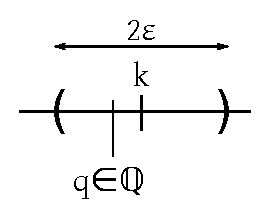
\includegraphics{img/dense_q.pdf}
      \caption{$k$ and an $\varepsilon$ environment}
    \end{center}
  \end{figure}
\end{theorem}
\begin{lemma}
  Let $A \subseteq \mathbb N$ and $A \neq \emptyset$.
  Then a minimum of $A$ exists.
\end{lemma}
\begin{proof}
  Proof by complete induction.

  We show: Let $A \subseteq \mathbb N$ such that no minimum exists.
  Then it holds that $A = \emptyset$.

  Let $C = \setdef{k \in \mathbb N}{\forall n \in A: k < n}$.
  $C$ is the set of all lower bounds of $A$ with operator $<$.
  We show: $0 \in C$ and $\forall k \in C \Rightarrow k + 1 \in C$.

  \begin{description}
    \item[Induction base]
      Assume $0 \not\in C$, hence for $k = 0$ it holds that
      \[ \exists n \in A \subset \mathbb N: n \leq 0 \]
      $\Rightarrow n \geq 0$ anyways and hence $n = 0$ and $0 \in A$.
      $\Rightarrow 0 = \min{A}$ and $A$ has a minimum.

      This is a contradiction. So $0 \not \in C$ does not hold.
      So $0 \in C$.
    \item[Induction step]
      Let $k \in C$, hence $\forall n \in A: k < n$.
      \[ \Rightarrow \forall n \in A: k + 1 \leq n \]
      Even $<$ holds. Assume $\exists n \in A: k + 1 = n$ and
      $\forall n' \in A: k + 1 \leq n'$.
      \[ \Rightarrow k + 1 \in A \land k + 1 \text{ is lower bound of } A \]
      Therefore $k + 1 = \min{A}$.

      This is a contradiction to the assumption that $\min{A}$ does not exist.
      Therefore $\forall n \in A: k + 1 < n \Rightarrow k + 1 \in C$.

      Due to the workings of induction: $\forall k \in \mathbb N: k \in C$
      equivalently means $C = \mathbb N$.

      Therefore $A = \emptyset$ holds.
      Assume $m \in A$, so it holds that $m \not\in C$, because $\neg (m < m)$.
  \end{description}
\end{proof}

\begin{proof}
  Case distinction:
  \begin{description}
    \item[$x > 0$]
      Let $\varepsilon > 0$ be arbitrary.
      Choose $n \in \mathbb N_+$ such that $\frac1n < \varepsilon$
      and define $A = \setdef{k \in \mathbb N}{k > n \cdot x}$.

      We know that $A \neq \emptyset$ (Archimedian axiom).
      Let $M = \min{A}$, then it holds that $m > n \cdot x$ and $m - 1 \leq n \cdot x$.
      Therefore $x < \frac mn$ and $x \geq \frac{m-1}{n}$.
      Therefore it holds that
      \[
        \abs{x - \frac mn} = \frac mn - x \leq \frac mn - \frac{m-1}{n}
        = \frac{m - m + 1}{n} = \frac 1n < \varepsilon
      \]
      and $\frac mn = q \in \mathbb Q$.
    \item[$x < 0$]
      Therefore $-x > 0$ and $\exists q \in \mathbb Q$:
      \[ \abs{q - (-x)} < \varepsilon \]
      \[ \abs{x + q} = \abs{x - \underbrace{(-q)}_{\in \mathbb Q}} \]
    \item[$x = 0$]
      Let $q = 0 \in \mathbb Q$.
  \end{description}
\end{proof}
\index[English]{dense in $\mathbb R$}
\index[German]{Dicht in $\mathbb R$}
\begin{cor}
  $\forall x \in \mathbb R$ and $\forall \varepsilon > 0$ it holds that
  \[
    \mathbb Q \cap B(x, \varepsilon)
    = \mathbb Q \cap (x - \varepsilon, x + \varepsilon)
    \neq \emptyset
  \]
  Therefore $x$ is a contact point of $\mathbb Q$.

  \textbf{Remark.}
  It even holds that $x$ is limit point of $\mathbb Q$.
  \[
    \overline{\mathbb Q}
      = \setdef{x \in \mathbb R}{x \text{ is contact point of } \mathbb Q}
      = \mathbb R
  \]
  We say $\mathbb Q$ is \emph{dense} (or: lies in) in $\mathbb R$.

  Alternative characterization of contact points:
  \[
    \forall x \in \mathbb R \exists (q_n)_{n \in \mathbb N}
    \text{ with } q_n \in \mathbb Q
    \text{ with } \lim_{n \to \infty} q_n = x
  \]
\end{cor}

\subsection{Intervals}
\meta{lecture}{5th of November 2015}{Wolfgang Ring}

\begin{defi}[Intervals]
  Let $a, b \in K$.
  \[ (a,b) = \setdef{x \in K}{(x > a) \land (x < b)} \]
  \[ [a, b) = \setdef{x \in K}{(x \geq a) \land (x < b)} \]
  \[ (a, b] = \setdef{x \in K}{(x > a) \land (x \leq b)} \]
  \[ [a, b] = \setdef{x \in K}{(x \geq a) \land (x \leq b)} \]
\end{defi}

\index[English]{interval length}
\index[German]{\foreignlanguage{ngerman}{Intervalllänge}}
\index[English]{open interval}
\index[German]{\foreignlanguage{ngerman}{Offenes Intervall}}
\index[English]{closed interval}
\index[German]{\foreignlanguage{ngerman}{Geschlossenes Intervall}}

\begin{theorem}[Laws for intervals]
  \begin{align}
    (a, b) &= \emptyset \text{ if } b \leq a \\
    [a, b] &= \emptyset \text{ if } b < a \\
    [a, a] &= \set{a}
  \end{align}
  If $I$ is an non-empty interval (hence $I \neq \emptyset$),
  then $\abs{I} = b - a$ is called \emph{length of the interval}.
  Furthermore
  \begin{align}
    (a, \infty) &= \setdef{x \in K}{x > a} \\
    [a, \infty) &= \setdef{x \in K}{x \geq a} \\
    (-\infty, a) &= \setdef{x \in K}{x < a} \\
    (-\infty, a] &= \setdef{x \in K}{x \leq a}
  \end{align}
\end{theorem}

\begin{theorem}
  $\mathbb Q$ is arithmetically incomplete.
\end{theorem}

\begin{proof}
  We define a mapping from $\mathbb N_+$ to $\mathbb N$:
  Let $n \in \mathbb N_+$ then we know that $n$ can be represented distinctly
  as product of prime numbers. Let $\operatorname{Z}(n)$ be the number of twos
  in the prime product representation.

  Examples:
  \[ \operatorname{Z}(14) = \operatorname{Z}(2 \cdot 7) = 1 \]
  \[ \operatorname{Z}(15) = \operatorname{Z}(3 \cdot 5) = 0 \]
  \[ \operatorname{Z}(24) = \operatorname{Z}(2 \cdot 2 \cdot 2 \cdot 3) = 3 \]

  It holds that $\operatorname{Z}(2n) = \operatorname{Z}(n) + 1 \forall n \in \mathbb N_+$
  and $\operatorname{Z}(n^2) = \operatorname{Z}(n) \cdot 2 \forall n \in \mathbb N_+$.

  We claim,
  \[ \not\exists q: q = \frac mn \text{ with } q^2 = 2 \]
  Proof by contradiction:
  \begin{enumerate}
    \item Assume $\left(\frac mn\right)^2 = 2$.
    \item Then $\frac{m^2}{n^2} = 2$.
    \item Then $m^2 = 2 \cdot n^2$.
    \item With $Z(m^2) = 2\cdot \operatorname{Z}(n)$.
    \item With $\operatorname{Z}(2\cdot n^2) = \operatorname{Z}(n^2) + 1 = 2 \cdot \operatorname{Z}(n) + 1$.
    \item If $m^2 = 2n^2$, then $\operatorname{Z}(m^2)$ must be even and $\operatorname{Z}(2\cdot n^2)$ must be odd.
    \item Then equality cannot be satisfied \lightning
  \end{enumerate}
\end{proof}

\subsection{Archimedean property and Completeness axiom}
\begin{theorem}
  $\mathbb Q$ is geometrically incomplete.

  We consider an infinite straight number line.
  We define $\mathbb R$ as ordered field with properties:
  \begin{description}
    \item[Archimedean property]
      $\mathbb N \subseteq \mathbb R$ with $\forall x \in \mathbb R: \exists n \in \mathbb N: x < n$

      \[ \mathbb N \subseteq \mathbb R \forall n \in \mathbb N: -n \in \mathbb N \]
      \[ \Rightarrow \forall n \in \mathbb N_+: n^{-1} \in \mathbb R \]
      \[ \Rightarrow \mathbb Z \subseteq \mathbb R \]

      Therefore $\forall m \in \mathbb N: m \cdot \frac1n = \frac mn \in \mathbb R
      \Rightarrow \mathbb Q \subseteq \mathbb R$.

      \begin{defi}
        Let $I_0, I_1, \dots, I_z$. $(I_n)_{n \in \mathbb N}$ is a sequence of closed intervals with
        \begin{enumerate}
          \item $\forall a \in \mathbb N: I_{n+1} \subseteq I_n$
          \item $\forall \varepsilon > 0 \exists n \in \mathbb N: n \geq N \Rightarrow \abs{I_n} < \varepsilon$
        \end{enumerate}
      \end{defi}

    \item[Completeness axiom]
      Let $(I_n)_{n \in \mathbb N}$ be nested intervals in $\mathbb R$.
      Then there exists some $x \in \mathbb R: x \in I_n: \forall n \in \mathbb N_+$.

      Be aware, there exists only \emph{one} $x \in \mathbb R$ with the property:
      $x \in I_n \forall n \in \mathbb N$.

      Assume $x \in I_n$ and $y \in I_n \forall n \in \mathbb N$ and $x \neq y$.
      \[ \abs{\beta - \alpha} \leq b - a = \abs{I} \]

      \begin{proof}
        Without loss of generality: $\alpha \leq \beta$.
        Then it holds that $\abs{\beta - \alpha} = \beta - \alpha \leq \beta
        + (-\alpha) \leq b + (-\alpha) = b - a = \abs{I}$.
        \[ a \leq \alpha \Rightarrow -a \geq -\alpha \]

        Consider arbitrary small $\varepsilon > 0$ and $N \in \mathbb N$ sufficiently large,
        such that $\abs{I_n} < \varepsilon$. Because $x,y \in I_n \Rightarrow
        \abs{x - y} < \varepsilon \Rightarrow x = y$.
      \end{proof}
  \end{description}
\end{theorem}

\begin{cor}
  From the Archimedean property it follows that,
  \[ \forall \varepsilon > 0: \exists N \in \mathbb N: n \geq N \Rightarrow \frac1n < \varepsilon \]
\end{cor}

\begin{proof}
  Let $x > \frac1\varepsilon \in \mathbb R$.
  Archimedean property: $\exists N \in \mathbb N: N > x$.

  For $n \geq \mathbb N$ it holds that $n > x > 0 \Rightarrow \frac1n < \frac1x = \varepsilon$.
\end{proof}

\begin{cor}
  Let $p \in \mathbb R, p > 1 \forall x \in \mathbb R: n \geq N \Rightarrow p^n > x$.
\end{cor}

\begin{proof}
  $p > 1 + u$ with $u = p - 1$
  \[ p^n = (1 + u)^n \underbrace{>}_{\text{Bernoulli}} 1 - nu = 1 + n(p-1) \]
  Let $x \in \mathbb R$ arbitrary, select $N \in \mathbb N: \frac{x-1}{p-1} < N$.

  Then it holds for $n \geq N:$
  \[
    \frac{x-1}{\underbrace{p-1}_{>0}}
    \Leftrightarrow x - 1 < n\cdot(p-1)
    \Leftrightarrow x < 1 + n(p-1) < p^n
  \]
\end{proof}

\begin{theorem}
  Let $q \in \mathbb R$ with $\abs{q} < 1$. Then it holds that
  \[
    \forall \varepsilon > 0 \exists N \in \mathbb N:
    n \geq N \Rightarrow \abs{q^n} = \abs{q}^n < \varepsilon
  \]
\end{theorem}

\begin{proof}
  Let $s = \abs{q} \geq 0$. Consider $q > 0$. Then
  \begin{align*}
    q^n &= 0 \\
    \abs{q^n} &= 0 \\
    \abs{q}^n &< \varepsilon \forall \varepsilon > 0 \forall n \in \mathbb N
  \end{align*}

  Let $q \neq 0$, then $0 < s < 1$. Let $p = \frac1s \Rightarrow p > 1$.
  Choose arbitrary $\varepsilon > 0$ and $x = \frac1\varepsilon$.
  Because of the Completeness axiom
  \[ \exists N \in \mathbb N: n \geq N \Rightarrow p^n > X \]
  So it holds that
  \[ \frac1{p^n} = S^n < \frac1x = \varepsilon \forall n \geq N \]
  \[ \Rightarrow \left(\abs{q}\right)^n = \abs{q^n} \]
\end{proof}

\begin{theorem}
  Let $x \in \mathbb R, x > 0$ and let $k \in \mathbb N_+$.
  Then there exists a distinct $y \in \mathbb R$ with $y \geq 0$
  such that
  \[ y^k = x \]
  We denote $y = \sqrt[k]{x}$ and conclude there exists $k$-th root numbers.
\end{theorem}

\begin{proof}
  Idea: Construct nested intervals.

  $(I_n)_{n \in \mathbb N}$ such that $y \in \bigcap_{n \in \mathbb N} I_n$
  satisfies the property that $y^k = x$.

  \[ 0 \leq y_1 < y_2 \Rightarrow y_1^k < y_2^k \]

  We define $J_0 = [a_0, b_0]$ with $a_0 = 0$ and $b_0 = 1 + x$.
  Then it holds that
  \[ a_0^k = 0^k = 0 \leq x \]
  \[ b_0^k = (1 + x)^k = 1 + k_n + \binom{k}{2} x^2 + \dots + x^k \geq 1 + kx > 0 \]
\end{proof}

\meta{lecture}{6th of November 2015}{Wolfgang Ring}

\begin{theorem}
  We prove:
  \[ 0 \leq y_1 < y_2 \Rightarrow y_1^k \leq y_2^k \]
\end{theorem}
\begin{proof}
  A short proof by a student:
  \begin{description}
    \item[$\mathbf{k = 2}$]
      \[ y^{k+1} = y^k \cdot y < y_2^k x < y_2^k y_2 = y^{k+1} \]
    \item[$\mathbf{k \rightarrow k + 1}$]
      \[ y_1^2 < y_2^2 \]
  \end{description}
\end{proof}

\begin{theorem}
  Let $a, b \in K$ and $k \in \mathbb N$.
  Then it holds that
  \[ a^k - b^k = (a - b)\left(\sum_{j=0}^{k-1} a^{k-1-j} b^j\right) \]
  \[ a^2 - b^2 = (a - b)(a + b) \]
  \[ a^3 - b^3 = (a - b)(a^2 + ab + b^2) \]
\end{theorem}

\begin{proof}
  \[
    (a - b)\left(\sum_{j=0}^{k-1} a^{k-j-1} b^j\right)
    = \sum_{j=0}^{j-1} a^{k-j} b^j - \sum_{j=0}^{k-1} a^{k-j-1} b^{j+1}
  \] \[
    = a^k + \sum_{j=1}^{k-1} a^{k-j} b^j - \underbrace{b^{k-1}}_{j=k-1} - \sum_{j=0}^{k-2} a^{k-j-1} b^{j+1}
  \] \[
    = a^k - b^k + \sum_{j=1}^{k-1} a^{k-j} b^j - \sum_{l=1}^{k-1} a^{k-l} b^l
  \] \[
    = a^k
  \]
\end{proof}

\begin{theorem}
  Let $y_2 > y_1$ then
  \[ y_2^k - y_1^k = \underbrace{(y_2 - y_1)}_{> 0} \underbrace{\left(\sum_{j=0}^{k-1} y_2^{k-j-1} y_1^j\right)}_{> 0} \]
  \[ \Rightarrow y_2^k - y_1^k > 0 \]
\end{theorem}

\begin{proof}
  \[ \forall x \geq 0 \in \mathbb R: \exists y \geq 0 \in \mathbb R: y^k = x \text{ with } k \in \mathbb N_+ \]
  Special case $x = 0$ and $y = 0$ is the solution.

  Let $x > 0$: We construct $y$ with $y \in \bigcap_{k=0}^\infty I_n$
  where $I_n$ are nested intervals.
  Specifically $I_n$ must have the properties:
  \begin{itemize}
    \item $I_n = [a_1, b_n]$ with $a^k \leq x, b_n^k \geq x \quad \forall n \in \mathbb N$
    \item $I_{n+1} \subseteq I_n: \abs{I_n} = \frac12 \abs{I_{n+1}} = \left(\frac12\right)^n \abs{I_0}$
  \end{itemize}

  \[ n = 0 \qquad I_0 = [0, x-1] \]
  \[ a_0 = b \qquad b_0 = x + 1 \]
  \[ a_0^k = 0 < x \qquad\checkmark \]
  \[ b_0^k = (1 + x)^k = 1 + kx + \binom k2 x^2 + \dots + x^k > 1 + kx > x \text{ for } k \geq 1 \]

  Let $I_n$ be given: $I_n = [a_n, b_n]$.
  Define $m_n = \frac12 (a_n + b_n)$
  \begin{description}
    \item[Case 1]
      \[ m_n^k \geq x \Rightarrow \text{ let } a_{n+1} = a_n, b_{n+1} = m \]
      \[ I_{n+1} = [a_n, m_n] \subseteq [a_n, b_n] = I_n \]
      \[ \abs{I_{n+1}} = m_n - a_n = \frac12 a_n + \frac12 b_n - a_n \]
      \[ \frac12 (b_n - a_n) = \frac12 \abs{I_n} \]
      \[ a_{n+1}^k = a^k \leq x \quad\checkmark \]
      All conditions are satisfied.
    \item[Case 2] $m_n^k < x: $
      Let $a_{n+1} = m_1, b_{n+1} = b_n$.
      It holds that $a_{n+1} = m_n < x, b_{n+1} = b_n \geq x \quad\checkmark$.
      Furthermore it holds that $I_{n+1} \subseteq I$ and $\abs{I_{n+1}} = \frac12 \abs{I_n}$.

      $I_n$ is set of nested intervals.
      Let $\varepsilon > 0$ be arbitrary. Then
      \[ \exists N \in \mathbb N: n \geq N \Rightarrow \left(\frac12\right)^n < \frac{\varepsilon}{1 + x} \]

      For those $n \geq N$ it holds that
      \[
          \abs{I_n} = \left(\frac12\right)^n \abs{I_{0}}
          = \left(\frac12\right)^n (x + 1)
          < \frac{\varepsilon}{1 + x} \cdot (1 + x)
      \]

      Let $y \in I_n \forall n \in \mathbb N$.
      Further nesting of intervals:
      \[ (I_n)_{n \in \mathbb N} \text{ with } I_n = [a_n^k, b_n^k] \]
      It holds that
      \[
          a_n \leq a_{n+1} < b_{n+1} \leq b_n \text{ because } I_{n+1} \subseteq I_n
          \Rightarrow a_n^b \leq a_{n+1}^k < b_{n+1}^k \leq b_n^k
      \]

      Length of $I_n$:
      \[ I_n = b_n^k - a_n^k = (b_n - a_n) \sum_{j=0}^{k-1} a_n^{k-1-j} b_n^j \]
      Because $I_n \leq I_0 \Rightarrow a_n < b_0 \Rightarrow b_n \leq b_0$,
      \[ < (b_n - b_0) \sum_{j=0}^{k-1} b_0^{k-1-j} b_0^{j} \]
      \[ = (b_n - a_n) k b_0^k = (b_n - a_n) k (1 + x)^k \]

      Let $\varepsilon > 0$ be arbitrary. Find some $N \in \mathbb N$ with $n \geq N$:
      \[ \abs{I_n} = (b_n - a_n) < \frac{\varepsilon}{k (1 + x)^k} \]
      For those $n$ it holds that
      \[ \abs{I_n} < \abs{I_n} \cdot k (1 - x)^k < \frac{\varepsilon}{k (1 + x)^k} k (1 + x)^k = \varepsilon \]

      Therefore $(I_n)_{n \in \mathbb N}$ a set of nested intervals.

      $\exists z \in \mathbb R$ with $z \in \lfloor a_n^k, b_n^k\rfloor: \forall n \in \mathbb N$
      and $z$ is unique. By construction of $I_n$ it holds that $a_n^k \leq x \leq b_n^k$
      \[ \Rightarrow x \in I_n \forall n \in \mathbb N \Rightarrow x = z \in \bigcap_{n \in \mathbb N} I_n. \]

      On the opposite side it holds that $y \in I_n$ (hence $a_n \leq y \leq b_n \Rightarrow a_n^k \leq y^k \leq b_n^k$).
      So $y^k \in I_n \forall n \in \mathbb N \Rightarrow y^k = z = x$.
      So we have found some $y^k$ which is $x$. But is $y \geq 0$ with $y^k = x$ unique?

      Let $y_1 \neq y_2$ with $y_1^k = y_2^k = x$ and without loss of generality,
      \[ 0 \leq y_1 < y_2 \Rightarrow y_1^k < y_2^k \quad\lightning \]
      So, $y$ is unique.
  \end{description}
\end{proof}

\section{Supremum property of $\mathbb R$}
\subsection{Boundedness in $\mathbb R$}
\index[English]{bounded}
\index[German]{\foreignlanguage{ngerman}{beschränkt}}
\index[English]{bounded below}
\index[German]{\foreignlanguage{ngerman}{beschränkt nach unten}}
\index[English]{bounded above}
\index[German]{\foreignlanguage{ngerman}{beschränkt nach oben}}
\index[English]{lower bound}
\index[English]{upper bound}
\begin{defi}
  Let $A \subseteq \mathbb R$.
  \begin{itemize}
    \item We call $A$ to be \emph{bounded above} if there exists some $u \in \mathbb R$ such that $\forall a \in A: a \leq u$.
    \item A number $u$ with that property is called \emph{upper bound of $A$}.
    \item We call $A$ to be \emph{bounded below} if there exists some $l \in \mathbb R$ such that $\forall a \in A: a \geq l$.
    \item A number $l$ with that property is called \emph{lower bound of $A$}.
    \item $A$ is called \emph{bounded} if there exists a lower and upper bound of $A$.
  \end{itemize}
\end{defi}

\begin{cor}
  Let $(a, b)$ be bounded.
  Let $u$ be its upper bound and let $v \geq u$.
  Then $v$ is also an upper bound of $(a, b)$.
\end{cor}

\meta{lecture}{11th of November 2015}{Wolfgang Ring}

\subsection{Supremum and infimum in $\mathbb R$}
\index[English]{supremum}
\index[German]{\foreignlanguage{ngerman}{Supremum}}
\index[English]{infimum}
\index[German]{\foreignlanguage{ngerman}{Infimum}}
\begin{defi}
  Let $A$ be bounded above.
  Assume $s \in \mathbb R$ has the properties
  \begin{enumerate}
    \item $s$ is an upper bound for $A$
    \item $\forall \sigma \in \mathbb R: \sigma < S$: $\sigma$ is not an upper bound for $A$.
  \end{enumerate}
  If those properties are satisfied, we call $s$ \emph{supremum of $A$}.
  A supremum $s$ is always the smallest upper bound of $A$.
  We denote $s = \sup{A}$.

  There exists at most one supremum for $A$. Let $s_1$ and $s_2$ be two suprema,
  then $s_1 \neq s_2$. So wlog. $\sigma_1 < \sigma_2$. This invalidates the supremum
  property of $s_2 \Rightarrow s_1$ is not a supremum of $A$ \lightning.

  Analogously an \emph{infimum of $A$} is the greatest lower bound of $A$.
  Let $A$ be bounded below. $t \in \mathbb R$ is called \emph{infimum of $A$}
  if
  \begin{enumerate}
    \item $\forall a \in A: t \leq a$ (t is a lower bound of $A$)
    \item $\forall x > t$ so $x$ is no lower bound of $A$
      \[ \Leftrightarrow \exists a \in A: a < x \]
  \end{enumerate}
  We denote $t = \inf{A}$.
\end{defi}

\begin{defi}
  Let $A \subseteq \mathbb R$. We denote $u = \max{A}$ for the \emph{maximum of $A$} if
  \begin{enumerate}
    \item $u \in A$ (is element of $A$)
    \item $\forall a \in A: a \leq u$ (is an upper bound)
  \end{enumerate}
  $l \in \mathbb R$ denoted $l = \min{A}$ is called minimum of $A$ if
  \begin{enumerate}
    \item $l \in A$ (is element of $A$)
    \item $\forall a \in A: l \leq a$ ($l$ is a lower bound)
  \end{enumerate}
\end{defi}

\begin{theorem}
  Let $A \subseteq R$ and $u$ be the maximum of $A$. Then it holds that
  $u = \sup{A}$. If $l = \min{A} \Rightarrow l = \inf{A}$.
\end{theorem}

\begin{proof}
  We need to show, that $l$ is an upper bound of $A$.
  This follows by definition.
  For $x < u$ it holds that $x$ not an upper bound.

  Let $x < u$, because $u \in A$ there exists some element $y$ in $A$
  with $y > x$. Therefore $x$ is not an upper bound of $A$.
\end{proof}

\begin{ex}
  \[ A = \set{1, \frac12, \frac13, \ldots} = \set{\frac1n: n \in \mathbb N_+} \]
  Then it holds that $1 \in A$ and $1 \geq \frac1n \forall n \in \mathbb N_+$.
  Therefore $1 = \max{A} = \sup{A}$.

  $0 = \inf{A}$, because $0$ is a lower bound of $A$ ($\frac1n > 0 \forall n \in \mathbb N_+$).
  Let $\varepsilon > 0$, then $\exists N \in \mathbb N: n \geq N
  \Rightarrow \frac1n \leq \varepsilon$. Therefore $\varepsilon$ is not a lower bound of $A$.

  So $A$ does not have a minimum, because otherwise $l = \max{A} = \inf{A} = 0$.
\end{ex}

\begin{theorem}
  Let $A \neq \emptyset$ and $A \subseteq \mathbb R$ be bounded above.
  So some $s = \sup{A} \in \mathbb R$ exists (therefore $\mathbb R$ has a supremum property).
\end{theorem}

\begin{proof}
  We construct nested intervals $(I_n){{n \in \mathbb N}}$ such that
  for $s \in \bigcap_{n \in \mathbb N} I_n$ gilt $s = \sup{A}$.
  We construct $I_{n+1}$ inductively using $I_n$

  \begin{description}
    \item[Case $\mathbf{n = 0}$] \hfill{} \\
      Because $A \neq 0$, we select $a_0 \in A$.
      Because $A$ is bounded above, $\exists b_0 \in \mathbb R$
      such that $b_0$ is an upper bound of $A$.
      We define $I_0 = [a_0, b_0]$.
    \item[Case $\mathbf{n \rightarrow n + 1}$] \hfill{} \\
      Let $a_0 = b_0$, then it holds that $b_0$ is upper bound and $b_0 \in A$.
      We call that terminating condition.
      Therefore $b_0 = \max{A} = \sup{A}$ and the supremum was found.
      Instead of $n$ we use $n + 1$.
      Let $I_0 = [a_n, b_n]$ with $a_n \neq b_n$ and $a_n \in A$,
      $b_n$ is an upper bound of $A$. Furthermore it holds that
      \[ \abs{I_n} \leq \left(\frac12\right)^n \abs{I_0} \]

      Consider $I_{n+1}$ such that the same properties are satisfied.
      Let $m_1 = \frac12 (a_1 + b_1)$. It holds that $a_n < m_n < b_n$.

      \begin{description}
        \item[Case $\mathbf{m_n}$ is an upper bound of $\mathbf{A}$]
          Then we set $a_{n+1} = a_n \in A$ and
          $b_{n+1} = m_n$ is an upper bound of $A$.
          \[ \abs{I_{n+1}} = b_{n+1} + a_{n+1} = \frac12 (b_n + a_n) - a_n \]
          \[
            = \frac12 b_1 - \frac12 a_n = \frac12 \abs{I_n}
            \leq \left(\frac12\right)^n \abs{I_0}
            = \left(\frac12\right)^{n+1} \abs{I_n}
            \qquad \checkmark
          \]
        \item[Case $\mathbf{m_n}$ is not an upper bound of $\mathbf{A}$]
          Therefore $\exists x \in A$ with $x > m_n$.
          \begin{description}
            \item[Subcase $\mathbf{x = b_1}$]
              So $b_1$ is an upper bound.
              Therefore $x \in A$ and $x$ is upper bound.
              \[ x = \max{A} = \sup{A} \]
              We found the supremum.
            \item[Subcase $\mathbf{m_n < x < b_n}$]
              Let $a_{n+1} = x \in A$ and $b_{n + 1} = b_n$ is an upper bound
              and
              \[
                  I_{n + 1} = b_{n+1} - a_{n+1} - b_n - x
                  < b_n - m_n - b_n - \frac12 (b_n + a_n) + \frac12 (b_n - a_n)
              \] \[
                  = \frac12 \abs{I_n} \leq \left(\frac12\right)^{n+1} \abs{I_0}
              \]
              We have found supremum $s = \sup{A}$.
          \end{description}
          If in any case the terminating condition holds, then we have found
          the supremum.

          The remaining case is $\forall n \in \mathbb: a_n < b_n, a_n \in A, b_n$
          is upper bound of $A$.
          \[ \abs{I_n} = b_n - a_n \leq \left(\frac12\right)^n \abs{I_0} \]
          Consider $\varepsilon > 0$ and $N$ such that $n \geq N \Rightarrow
          \left(\frac12\right)^n < \frac{\varepsilon}{\abs{I_n}}$.
          For those $n$ it holds that
          \[ \abs{I_n} \leq \left(\frac12\right)^n \abs{I_0} < \frac{\varepsilon}{\abs{I_0}} \abs{I_0} = \varepsilon \]
          Therefore $(I_n)_{n \in \mathbb N}$ are nested intervals.
      \end{description}
  \end{description}
\end{proof}

What remains for completeness:
  $s \in \mathbb R, s \in I_n: \forall n \in N$.
  We need to show that $s = \sup{A}$.

\meta{lecture}{12th of November 2015}{Wolfgang Ring}

\begin{theorem}
  Completeness of $\mathbb{R}$:
  \[ \exists s \in \mathbb R: s \in I_n \forall n \in \mathbb N \]
\end{theorem}

\begin{proof}[\textbf{Proof} cont]
  Every set with an upper bound has a supremum.

  We construct $(I_n)_{n \in \mathbb N}$ with $I_n = [a_n, b_n]$ and $I_{n+1} \subseteq I_n$.
  $\forall n \in \mathbb N: a_n \in A$, $b_n$ is the upper bound of $A$.
  \[ \abs{I_{n+1}} \leq \frac12 \abs{I_n} \leq \left(\frac12\right)^{n+1} \abs{I_0} \]

  \begin{figure}[!h]
    \begin{center}
      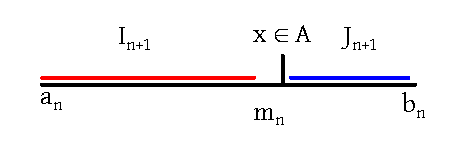
\includegraphics{img/proof_interval.pdf}
      \caption[width=200pt]{Relation of $a_n$ and $b_n$ and $J_{n+1}$}
    \end{center}
  \end{figure}

  Consider $I_{n+1} \subseteq I_n$ with $a_n < b_n \forall n \in \mathbb N$.
  \[ \abs{I_n} \leq \left(\frac12\right)^n \abs{I_0} \]

  \begin{figure}[!h]
    \begin{center}
      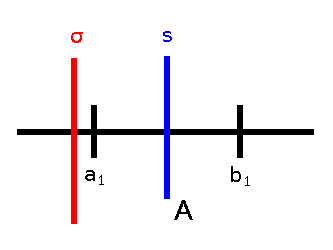
\includegraphics{img/proof_interval2.pdf}
      \caption[width=200pt]{Illustration of $s$ between $a_n$ and $b_n$}
    \end{center}
  \end{figure}

  \begin{enumerate}
    \item
      Claim: $s$ is $\sup{A}$.

      We need to show (by contradiction):
      $S$ is upper bound of $A$. Assume $a \in A$ and $a > s$.
      Let $\varepsilon = a - s > 0$ and choose $N$ sufficiently large such that
      \[ \abs{I_n} < \varepsilon = a - s \]
      Then it holds that
      \[
          b_N
          = \underbrace{b_n - a_n}_{\varepsilon} \not|
          \underbrace{a_N}_{< s} < s + \varepsilon
          = a
      \]
      \[ \Rightarrow b_N < a \in A \qquad\lightning \]
      Because $b_n$ is an upper bound.

    \item
      $\forall \sigma < s$ it holds that $\sigma$ is not an upper bound of $A$.
      Let $\sigma < s$ and $\varepsilon = s - \sigma > 0$ and choose $n \in N$
      large enough such that $b_N - a_N < \varepsilon$. Then it holds that
      \begin{align*}
        a_N &= a_N - b_N + b_N \\
            &> -\varepsilon + s \\
            &= -s + \sigma + s = \sigma \qquad \checkmark
      \end{align*}
      Therefore it holds that $s$ is smallest upper bound of $A$ and therefore
      supremum.
  \end{enumerate}
\end{proof}

\begin{theorem}
  Every set with a lower bound in $\mathbb R$ has an infimum.
  Every set with an upper bound in $\mathbb R$ has an supremum.
\end{theorem}

\begin{theorem}
  Remember that $M$ has the same cardinality like $A$ if $\varphi: M \rightarrow A$.
  $\varphi$ is bijective, $M$ is called countably infinite
  if $M$ has the same cardinality like $\mathbb N$.

  Let $\varphi: \mathbb N \rightarrow M$ be bijective therefore
  $M = \set{\varphi(1), \varphi(2), \varphi(3), \ldots} = \setdef{\varphi(n)}{n \in \mathbb N}$
  and $\varphi(i) \neq \varphi(j)$ for $i \neq j$.

  \textbf{Notation.} $\varphi(n) = m_n$.

  $M = \set{m_0, m_1, m_2, \ldots}$ with $m_i \neq m_j$ for $i \neq j$.
  $\varphi$ is a complete enumeration of all elements of $M$.

  Therefore every element of $M$ has the structure: $m_n$ with $i \in \mathbb N$.
\end{theorem}

\begin{theorem}
  \[ \mathbb Q^+ = \set{\frac mn, m \in \mathbb N, n \in \mathbb N_+} \]
  The set $\mathbb Q^+$ is countably infinite.
\end{theorem}

\begin{proof}
  We enumerate the elements of $\mathbb Q^+$.

  %\begin{table}[!h]
  %  \begin{center}
  %    \begin{tabular}{c|cccccccc}
  %        \multicolumn{8}{c}{Enumerator} \\
  %      Denominator: 1 & 1 & 2 & 3 & 4 & 5 & 6 & 7 & \ldots \\
  %        $2$ & $\frac12$ & $\frac22$ & $\frac32$ & $\frac42$ & $\frac52$ & $\frac62$ & $\frac72$ & \ldots \\
  %        $3$ & $\frac13$ & $\frac23$ & $\frac33$ & $\frac43$ & $\frac53$ & $\frac63$ & $\frac73$ & \ldots \\
  %        $4$ & $\frac14$ & $\frac24$ & $\frac34$ & $\frac44$ & $\frac54$ & $\frac64$ & $\frac74$ & \ldots \\
  %        $5$ & $\frac15$ & $\frac25$ & $\frac35$ & $\frac45$ & $\frac55$ & $\frac65$ & $\frac75$ & \ldots
  %    \end{tabular}
  %    \caption{
  %      A complete enumeration of $\mathbb Q^+$ (diagonalization argument)
  %      The enumeration goes as follows:
  %      $1 \rightarrow 0, 2 \rightarrow 1, \frac12 \rightarrow 2, \frac13 \rightarrow 3$
  %      and $\frac22$ is skipped, because it occurs already as $\frac22$.
  %      We traverse the whole matrix diagonally.
  %    }
  %  \end{center}
  %\end{table}
  \begin{figure}[!h]
    \begin{center}
      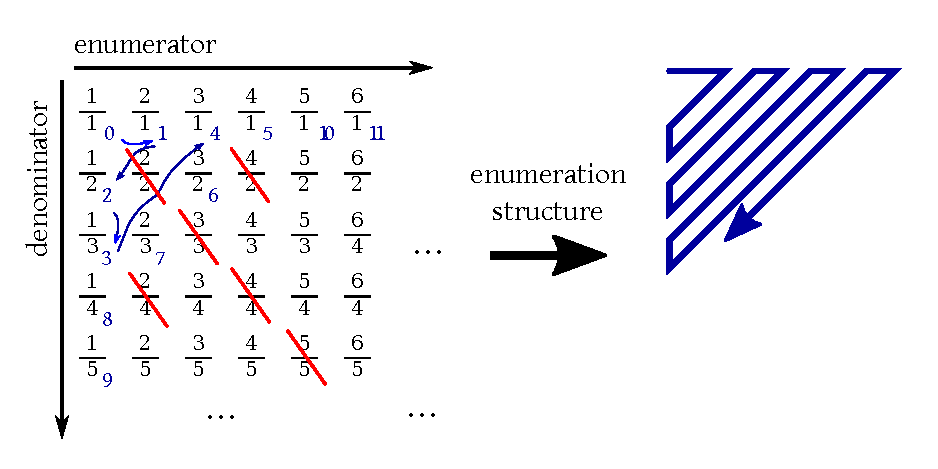
\includegraphics[width=0.5\textwidth]{img/enumeration_of_Q.pdf}
      \caption{
        A complete enumeration of $\mathbb Q^+$ (diagonalization argument).
        We traverse the whole matrix diagonally. The blue numbers indicate the
        enumeration and red lines cross out values already enumerated.
        On the right-hand side the general order of the enumeration is illustrated.
      }
    \end{center}
  \end{figure}

  \[ \mathbb Q_+ = \set{q_0, q_1, q_2, \ldots} \]
  \[ \mathbb Q_- = \set{-q_0, -q_1, -q_2, \ldots} \]
  \[ \mathbb Q = \set{0, q_0, -q_0, q_1, -q_1, \ldots} \]
  An enumeration exists. So $\mathbb Q$ is countably infinite.
\end{proof}

\index[English]{uncountability}
\index[English]{\begin{otherlanguage}{ngerman}überabzählbar\end{otherlanguage}}
\begin{theorem}
  There is no bijective relation $\varphi: \mathbb N \rightarrow \mathbb R$.
  Therefore we call $\mathbb R$ \emph{uncountable}.
\end{theorem}

\begin{proof}
  We provide a proof by contradiction.
  Assume $\mathbb R = \set{x_0, x_1, x_2, x_3, \ldots}$ is countable.

  We construct nested intervals.
  \begin{description}
    \item[Case $\mathbf{n = 0}$]
      \[ I_0 = \left[x_0 + 1, x_0 + 2\right] \]
      Let $\abs{I_0} = 1$ and $x_0 \not\in I_0$.

      \begin{figure}[!t]
        \begin{center}
          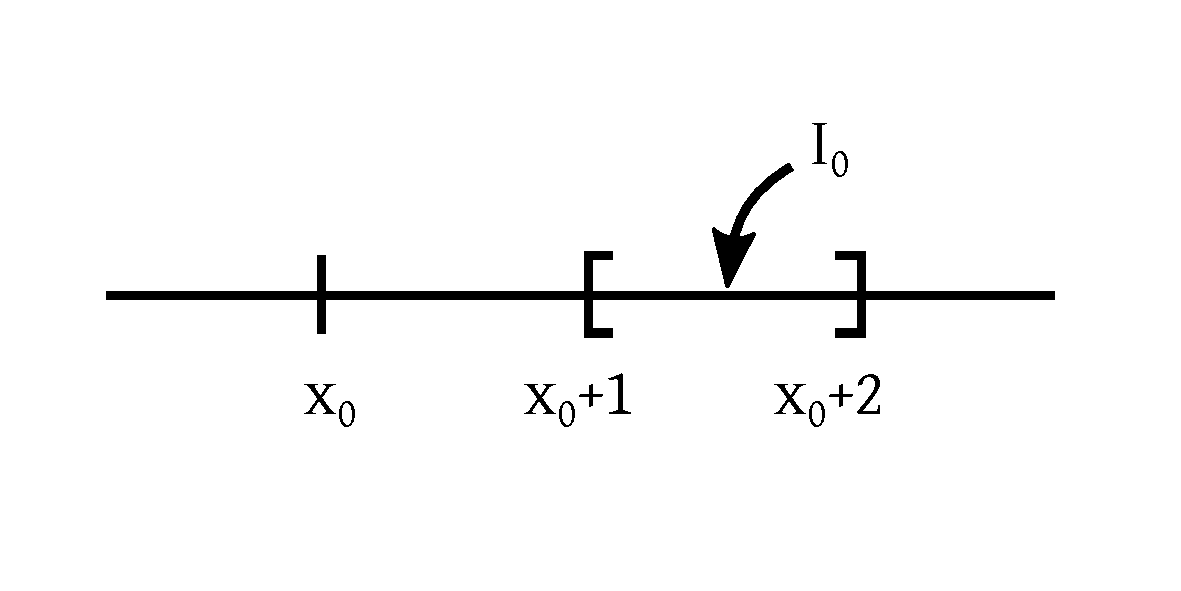
\includegraphics[width=200px]{img/interval_I0.pdf}
          \caption{Construction of a nested interval and its $I_0$}
        \end{center}
      \end{figure}

    \item[Case $\mathbf{n \rightarrow n + 1}$]
      Assume $I_{0} \dots I_n$ were already defined with $x_k \notin I_k$ for $0 \leq k \leq n$.
      \[ I_{k+1} \leq I_k \text{ for } k = 0, \dots, n-1 \]
      \[ \abs{I_k} = \left(\frac13\right)^k \]

      \begin{figure}[!t]
        \begin{center}
          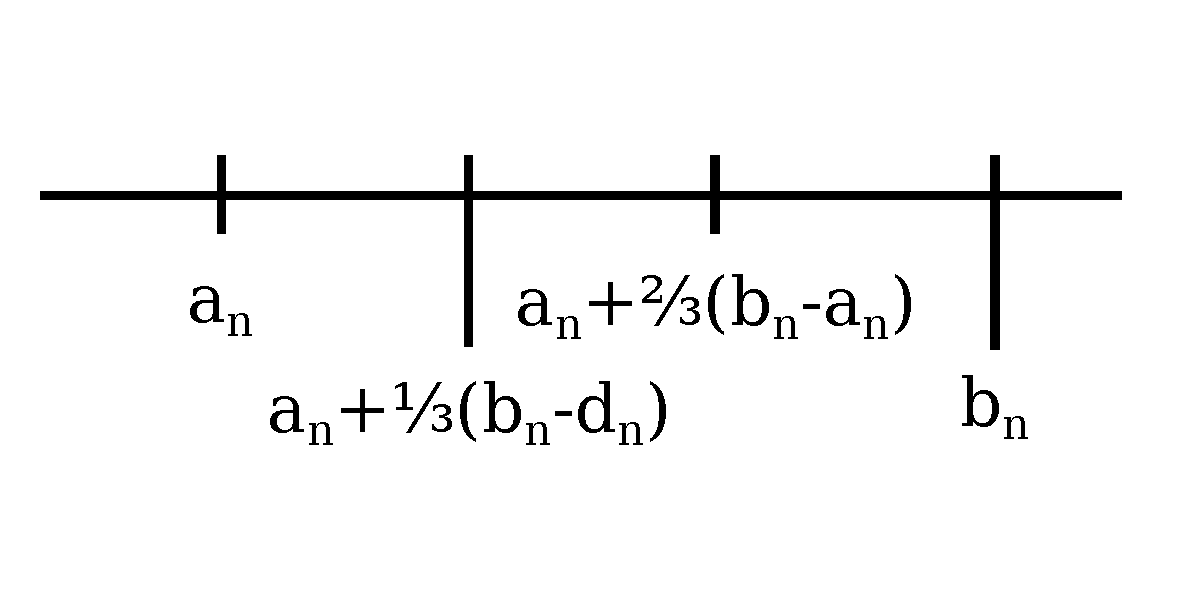
\includegraphics[width=200px]{img/interval_In.pdf}
          \caption{Construction of a nested interval and its $I_n$}
        \end{center}
      \end{figure}

      We construct $I_{n+1}$. Let $I_n = [a_n, b_n]$.
      \begin{align*}
        I_n^1 &= \left[a_n, \frac23 a_n + \frac13 b_n\right] \\
        I_n^2 &= \left[\frac23 a_n + \frac13 b_n, \frac13 a_n + \frac23 b_n\right] \\
        I_n^3 &= \left[\frac13 a_n + \frac23 b_n, b_n\right]
      \end{align*}
      So $x_n$ certainly is not contained in all three intervals $I_n^1$, $I_n^2$
      and $I_n^3$ because $I_n^1 \cap I_N^2 \cap I_N^3 = \emptyset$.
      Choose $I_{n+1}$ as one of the three intervals $I_n^l$ with $x_{n+1} \not\in I_n^l = I_{n+1}$.
      $I_{n+1} < I_n$.
      \[ \abs{I_{n+1}} = \frac13 I_{n} = \left(\frac13\right)^{n+1} \]
      For $\varepsilon > 0$ it holds that there exists some $N \in \mathbb N$
      such that $n \geq N \Rightarrow \abs{I_1} = \left(\frac13\right)^n < \varepsilon$.
      Therefore nested intervals $I_n$ are given.

      Let $x \in \mathbb R$ such that $\forall n \in \mathbb N: X \in I_n$
      (because of completeness law). Then it holds that $\forall x_n: x \neq x_n$.
      $x \in I_n$ and $x_n \not\in I_n$.
      Therefore $x \in \set{x_0, x_1, x_2, \ldots} = \mathbb R$.

      This contradicts with the assumption that $\mathbb R$ is countable.
  \end{description}
\end{proof}

\section[Complex numbers]{Complex numbers $\mathbb C$}

We introduce a new arithmetic unit denoted $i$, which extends the field $\mathbb R$.
Elements of $\mathbb C$ are represented as $a + bi$ with $a,b \in \mathbb R$.
\begin{align}
  \forall a, b \in \mathbb R: a + bi = 0 &\Leftrightarrow a = 0 \land b = 0 \\
  i^2 &= -1 \\
  \text{associativity,} & \text{ commutativity etc holds}
\end{align}

\meta{lecture}{13th of November 2015}{Wolfgang Ring}

\begin{defi}
  We consider an \enquote{arithmetic element} $i$ extending $\mathbb R$ (\enquote{adjungiert}). % TODO: translate to english
  Arithmetic operations are well-defined for $i$. Associativity and commutativity holds.
  It holds that
  \begin{itemize}
    \item $a + ib = 0$ with $a,b \in \mathbb R \Leftrightarrow a = 0 \land b = 0$
    \item $i^2 = -1$ i.e. $i^2 + 1 = 0$.
    \item Arithmetic operations still hold.
  \end{itemize}

  By the first law,
  \[
    a + ib = a' + ib' \Leftrightarrow (a - a') + i(b - b') = 0
    \Leftrightarrow a - a' = 0 \land b - b' = 0 \text{ therefore }
    a = a' \land b = b'
  \]

  By the second law, $i$ is the solution of the quadratic equation $i^2 + 1 = 0$.

  Let $z = a + ib$ a complex number. We call $i$ the \enquote{imaginary unit}.
  \[ \mathbb C = \set{z = a + ib : a,b \in \mathbb R} \]
  $\mathbb C$ is the field of complex numbers with the following properties:
  \begin{itemize}
    \item For addition, it holds that
      \[ (a + ib) + (c + id) = (a + b) + i (b + d) \subseteq \mathbb C \]
      and
      \[ (a + ib) + (-a - ib) = (a - a) + i(b - b) = 0 + i \cdot 0 = 0 \]
    \item For multiplication, it holds that
      \[ (a + ib) \cdot (c + id) = (ac + \underbrace{(i)^2}_{=-1} b d) + i (bc + ad) \]
      \[ (ac - bd) + i (bc + ad) \]
    \item Laws $\mathbf{A_n}$ to $\mathbf{A_4}$, $\mathbf{M_1}$ to $\mathbf{M_3}$ and $\mathbf{D}$ hold.
    \item The one element exists:
      \[ 1 = 1 + 0 \cdot i \]
      \[ (a + i \cdot b) (1 + i \cdot 0) = (a + (i)^2 \cdot 0) + i (b + 0) = a + ib \]
    \item \textbf{M4} holds: Let $z \in \mathbb C \setminus \set{0}$.
      Let $z = a + ib$ and $\neg(a = 0 \land b = 0) \Leftrightarrow a^2 + b^2 > 0$.
  \end{itemize}

  We define
  \[ w = \frac{a}{a^2 + b^2} - i \frac{b}{a^2 + b^2} \]
  \[ z \cdot w = \left(a + ib\right) \left(\frac{a}{a^2 + b^2} - i \frac{b}{a^2 + b^2}\right) \]
  \[
      = \left(\underbrace{\frac{a^2}{a^2 + b^2} - \frac{b \cdot (-b)}{a^2 + b^2}}_{=1}\right)
      + i \cdot \left(\underbrace{\frac{ba}{a^2 + b^2} - \frac{a\cdot b}{a^2 + b^2}}_{=0}\right)
  \] \[
    = 1 + i \cdot 0 = 1
  \]
  Therefore $w = z^{-1} = \frac1z$.

  Therefore $\mathbb C$ is a field.
\end{defi}

\begin{figure}[!ht]
  \begin{center}
    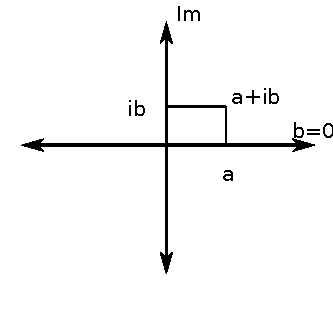
\includegraphics[width=200px]{img/complex_numbers_illustration.pdf}
    \caption{Illustration of complex numbers}
  \end{center}
\end{figure}
\begin{figure}[!ht]
  \begin{center}
    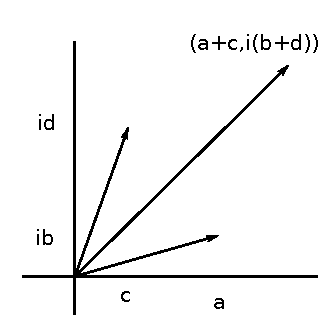
\includegraphics[width=200px]{img/complex_numbers_addition.pdf}
    \caption{Illustration of complex number addition}
  \end{center}
\end{figure}
\begin{figure}[!ht]
  \begin{center}
    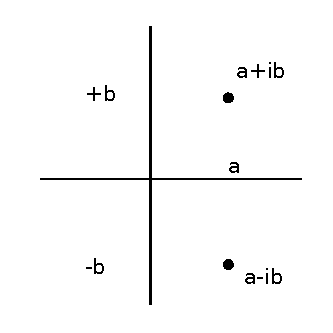
\includegraphics[width=200px]{img/complex_numbers_conjugate.pdf}
    \caption{Illustration of the complex conjugate}
  \end{center}
\end{figure}

We denote
\begin{align*}
  a &= \Re(z) \\
  b &= \Im(z) \\
  \overline{z} &= a - ib \\
  \abs{z} &= \sqrt{a^2 + b^2}
\end{align*}

$a$ is called \emph{real part of $z$}. $b$ is called \emph{imaginary part of $z$}.
$z$ is called complex conjugate. $\abs{z}$ is called absolute value of $z$.

\begin{theorem}
  \[  \overline{(\overline{z})} = z  \]
\end{theorem}

\begin{proof}
  \[ \overline{(\overline{z})} = \overline{(a - ib)} = (a - (-ib)) = a + ib  = z \]
\end{proof}

\begin{theorem}
  \[ \Re(z) = \frac12 (z + \overline z) \]
\end{theorem}

\begin{theorem}
  \[ \frac12(z + \overline{z}) = \frac12(a + ib + a - ib) = \frac12 (2a) = a \checkmark \]
\end{theorem}

\begin{theorem}
  \[ \Im(z) = \frac{1}{2i} (z - \overline{z}) \]
\end{theorem}

\begin{proof}
  \[ \frac{1}{2i} (a + ib - (a - ib)) = \frac{1}{2i} (2ib) = b \checkmark \]
\end{proof}

\begin{theorem}
  \[ z \in \mathbb R \Leftrightarrow z = \overline{z} \]
\end{theorem}
\begin{proof}
  \[ z = a \in \mathbb R \Rightarrow \overline{z} = a = z \]
  On the opposite, let $z = \overline{z}$ therefore
  \[ a = ib = a - ib \Rightarrow 2ib = 0 \Rightarrow b = 0 \]
  Therefore $z = a \in \mathbb R$.
\end{proof}

\begin{theorem}
  \[ z \in i \mathbb R = \set{ib : b \in \mathbb R} \Leftrightarrow z = -\overline{z} \]
  Proof follows analogously.
\end{theorem}

\begin{theorem}
  It holds that $\abs{z} = \sqrt{z \cdot \overline{z}}$.
\end{theorem}

\begin{proof}
  \[ \sqrt{z \cdot \overline{z}} = ((a + ib)(a - ib))^{\frac12} \]
  \[ = (a^2 - (ib)^2)^{\frac12} = (a^2 - i^2 b^2)^{\frac12} \]
  \[ = (a^2 + b^2)^{\frac12} = \abs{z} \quad\checkmark \]
\end{proof}

\begin{theorem}
  Let $z, w \in \mathbb C$:
  \[ \overline{(zw)} = \overline z \cdot \overline w \]
\end{theorem}

\begin{proof}
  \[ z = a + ib \qquad w = c + id \]
  \[ zw = (ac - bd) + i (bc + ad) \]
  \[ \overline{zw} = (ac - bd) - i (bc + ad) \]
  \[ \overline{zw} = a - ib \qquad \overline{w} = c - id \]
  \[
      \overline{z} \cdot \overline{w} = (ac - (-b) (-d)) + i (-bc + a(-d))
        = (ac - bd) - i (bc + ad)
  \]
\end{proof}

\begin{cor}
  \[ \overline{z + w} = \overline{z} + \overline{w} \]
\end{cor}

\begin{theorem}
  \[ \abs{zw} = \abs{z} \cdot \abs{w} \]
\end{theorem}
\begin{proof}
  \[ \abs{z \cdot w} = (zw) \cdot(\overline{z \cdot w})^{\frac12} \]
  \[
      = (z \cdot \overline z \cdot w \cdot \overline w)^{\frac12}
      = (z \cdot \overline z)^{\frac12} \cdot (w \cdot \overline w)^{\frac12}
      = \abs{z} \cdot \abs{w}
  \]
\end{proof}

\begin{theorem}
  \[ z = 0 \Leftrightarrow \abs{z} = 0 \in \mathbb R \]
\end{theorem}

\begin{proof}
  \[ z = 0 = 0 + i 0 \Rightarrow \abs{z} = \sqrt{0^2 + 0^2} = 0 \]
  Let $\abs{z} = \sqrt{a^2 + b^2} = 0 \Rightarrow a^2 + b^2 = 0$.
  \[ \Rightarrow a = 0 \land b = 0 \]
\end{proof}

\begin{theorem}
  \[ \abs{\Re(z)} = \abs{a} = \sqrt{a^2} \leq \sqrt{a^2 + b^2} = \abs{z} \]
  \[ \abs{\Im(z)} = \abs{b} = \sqrt{b^2} \leq \sqrt{a^2 + b^2} = \abs{z} = \]
\end{theorem}

\begin{theorem}
  The triangle inequality holds:
  \[ \forall z, w \in \mathbb C: \abs{z + w} \leq \abs{z} + \abs{w} \]
\end{theorem}

\begin{rem}
  Let $0 \leq y_1 < y_2$ with $y_1, y_2 \in \mathbb R$.
  Let $k \in \mathbb N_+$. Then it holds that
  \[ \sqrt[k]{y_1} < \sqrt[k]{y_2} \]
\end{rem}

\begin{proof}
  Indirect proof: Let $\sqrt[k]{y_1} \geq \sqrt[k]{y_2} \geq 0$.
  \[ \Rightarrow \left(\sqrt[k]{y_1}\right)^k \geq \left(\sqrt[k]{y_2}\right)^k \]
  therefore $y_1 \geq y_2$. This is the negation of our assumption.
\end{proof}

\begin{proof}[\textbf{Proof} of the triangle inequality]
  We show that $\abs{z + w}^2 \leq \left(\abs{z} + \abs{w}\right)^2$.
  \[
      \abs{z + w}^2 = (z + w)(\overline z + \overline w)
      = \underbrace{z \overline z}_{\abs{z}^2} + w \overline z
      + z \overline w + \underbrace{w \overline w}_{\abs{w}^2}
  \]
  \begin{align*}
      &= 2 \Re{(w \overline{z})} \\
      &= (w \overline{z} + \underbrace{\overline{(w \cdot \overline z)}}_{\overline w \cdot \overline z = \overline w \cdot z} \\
      &= \abs{z}^2 + 2\Re{(w \cdot \overline z)} + \abs{w}^2 \\
      &\leq \abs{z}^2 + 2\abs{\Re{(w \cdot \overline z)}} + \abs{w}^2 \\
      &\leq \abs{z}^2 + 2 \cdot \abs{w \cdot \overline{z}} + \abs{w}^2 \\
      &= \abs{z}^2 + 2 \cdot \abs{w} \cdot \abs{\overline{z}} + \abs{z}^2 \\
      &= \abs{z}^2 + 2 \cdot \abs{w} \cdot \abs{z} + \abs{w}^2 \\
      &= \left(\abs{z} + \abs{w}\right)^2
  \end{align*}
\end{proof}

\begin{theorem}
  In our previous proof there was a small loop hole: We need to show that
  \[ \abs{z} = \abs{\overline z} \]
\end{theorem}

\begin{proof}
  \[ \sqrt{a^2 + b^2} = \sqrt{a^2 + (-b)^2} = \sqrt{a^2 + b^2} \]
\end{proof}

\subsection{Interpretation of multiplication}
%
Multiplication with $i$. Let $z = a + ib$.
\[ iz = i\cdot a + i^2 \cdot b = (-b) + i a \]

\begin{figure}[!h]
  \begin{center}
    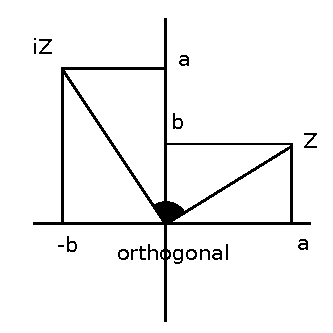
\includegraphics[width=200px]{img/complex_number_multiplication.pdf}
    \caption{Multiplication corresponds to a rotation by $90^\circ$}
  \end{center}
\end{figure}

Multiplication with $i$ rotates $z$ counter-clockwise by $90^\circ$
in the plane.

Let $z \in \mathbb C$ and $w = c + id$.

\begin{figure}[!h]
  \begin{center}
    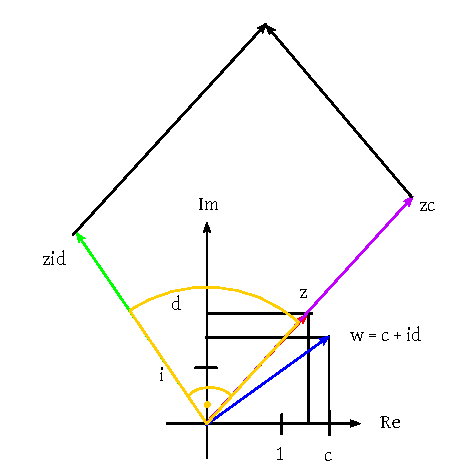
\includegraphics[width=200px]{img/complex_numbers_multiplication_with_b.pdf}
    \caption{
      In regards of multiplication with $w$ the complex number $z$ is scaled by $\abs{w}$
      and then rotated by an angle which is given between $w$ and the positive real axis.
      % Drehstreckung
    }
  \end{center}
\end{figure}

\meta{lecture}{18th of November 2015}{Wolfgang Ring}

\subsection{Taking roots}
%
\[ \forall a \in \mathbb R: a \geq 0 \forall n \in \mathbb N_+: \exists x \geq 0 \in \mathbb R: x^n = a \]

Taking the n-th root only works for positive integers, because $\forall x \geq 0: x^2 \geq 0$
and no solution in $\mathbb R$ exists for the equation $x^2 = -1$.

In $\mathbb C$ it holds that $\forall w \in \mathbb C \setminus \set{0}$.
$\forall n \in \mathbb N$ there exist exactly $n$ different solutions of the equation$ z^n = w$.

\section{Sequences of real and complex elements}
\index[English]{Sequences}
\index[German]{\foreignlanguage{ngerman}{Folge}}
\begin{defi}
  Let $a$ be a mapping $\mathbb N \rightarrow \mathbb R$ is called \emph{sequence} of real numbers.
  \[ \forall n \in \mathbb N: a(n) \in \mathbb R \]
  We denote $a_n \coloneqq a(n)$.
  Instead of $a: \mathbb N \rightarrow \mathbb C$ we write $(a_n)_{n \in \mathbb N} = (a_0, a_1, \ldots)$.

  Analogously for the complex numbers $\mathbb C$ and general sets $X$.
\end{defi}

\begin{ex}
  $a_n = \sqrt[n]{2} \frac{1}{n + 1}$ with $(a_n)_{n \in \mathbb N}$. Or simply:
  \[ \left(\sqrt[n]{2}\frac{1}{n + 1}\right)_{n \in \mathbb N} \]
\end{ex}

\begin{ex}
  Let $(I_n)_{n \in \mathbb N}$ be nested intervals.
  Therefore $(I_n)_{n \in \mathbb N}$ is a sequence of elements in $X = \set{[a,b]: a,b \in \mathbb R, a \leq b}$.
\end{ex}

\index[English]{bounded below}
\index[German]{\foreignlanguage{ngerman}{beschränkt nach unten}}
\index[English]{bounded above}
\index[German]{\foreignlanguage{ngerman}{beschränkt nach oben}}
\index[English]{bounded}
\index[German]{\foreignlanguage{ngerman}{beschränkt}}
\begin{defi}
  Let $(a_n)_{n \in \mathbb N}$ be a real sequence.
  $(a_n)_{n \in \mathbb N}$ is called \emph{bounded above} if $o \in \mathbb R$ exists such that $\forall n \in \mathbb N: a_n \leq o$.
  $(a_n)_{n \in \mathbb N}$ is called \emph{bounded below} if $u \in \mathbb R$ exists such that $\forall n \in \mathbb N: a_n \geq u$.

  $(a_n)_{n \in \mathbb N}$ is called bounded, if $(a_n)_{n \in \mathbb N}$ is bounded above and below.
\end{defi}

\index[English]{Monotonic function}
\index[German]{\foreignlanguage{ngerman}{Monotonie}}
\index[English]{Monotonically increasing}
\index[German]{\foreignlanguage{ngerman}{Monoton ansteigend}}
\index[English]{Strictly monotonically increasing}
\index[German]{\foreignlanguage{ngerman}{Streng monoton steigend}}
\index[English]{Monotonically decreasing}
\index[German]{\foreignlanguage{ngerman}{Monoton abfallend}}
\index[English]{Strictly monotonically decreasing}
\index[German]{\foreignlanguage{ngerman}{Streng monoton fallend}}
\begin{ex}
  $(a_n)_{n \in \mathbb N}$ with $a_n = \frac{n}{n+1}$ is bounded below by $0$
  and bounded above by $1$: $n \leq n+1 \Rightarrow n \frac{1}{n+1} < \frac{n+1}{n+1} = 1 \checkmark$.
\end{ex}

\subsection{Monotonicity}
\begin{defi}\hfill{}
  \begin{itemize}
    \item $(a_n)_{n \in \mathbb N}$ is called \emph{monotonically increasing} if $\forall n \in \mathbb N: a_{n+1} \geq a_n$.
    \item $(a_n)_{n \in \mathbb N}$ is called \emph{monotonically decreasing} if $\forall n \in \mathbb N: a_{n+1} \leq a_n$.
    \item $(a_n)_{n \in \mathbb N}$ is called \emph{monotonically strictly increasing} if $\forall n \in \mathbb N: a_{n+1} > a_n$.
    \item $(a_n)_{n \in \mathbb N}$ is called \emph{monotonically strictly decreasing} if $\forall n \in \mathbb N: a_{n+1} > a_n$.
  \end{itemize}
  In $\mathbb C$, elements are not ordered, so we need to define an order explicitly.
  Let $(a_n)_{n \in \mathbb N}$ a complex sequence. We define:
  \begin{itemize}
    \item $(a_n)_{n \in \mathbb N}$ is called bounded if $(\abs{a_n})_{n \in \mathbb N}$ is a bounded real sequence.
    Hence $\exists o \in \mathbb R: \forall n \in \mathbb N: \abs{a_n} \leq o$.
    \item The lower bound is implicitly given by $0$.
  \end{itemize}
\end{defi}

\begin{ex}
  $a_n \coloneqq i^n$ and $(a_n)_{n \in \mathbb N} = (1, i, -1, -i, 1, i, -1, -i, 1, i, -1, \dots)$
  \[ \abs{1} = 1 \qquad \abs{-1} = 1 \qquad \abs{i} = \sqrt{0^2 + 1^2} = 1 \qquad \abs{-i} = \sqrt{0^2 + (-1)^2} = 1 \]
  So $\left(\abs{a_n}\right)_{n \in \mathbb N} = (1, 1, 1, 1, 1, \dots)$.
  It holds that
  \[ \abs{z} = \abs{-z} = \abs{\overline{z}} \]
\end{ex}

\index[English]{convergent}
\index[German]{\foreignlanguage{ngerman}{Konvergent}}
\index[English]{divergent}
\index[German]{\foreignlanguage{ngerman}{Divergent}}
\begin{defi}
  Let $\seq{a_n}$ be a sequence of $\mathbb C$ and let $a \in \mathbb C$.
  We state: $(a_n)_{n \in \mathbb N}$ has a limit (lat. limes) $a$ if
  \[ \forall \varepsilon > 0 \exists N \in \mathbb N: \left[n \geq N \implies \abs{a_n - a} < \varepsilon\right] \]
  We denote
  \[ \lim_{n \to \infty} a_n = a \]
  The distance $\abs{a_n - a}$ becomes arbitrary small, if $n$ is sufficiently large.

  A sequence, which has a limit, is called \emph{convergent}. A sequence, which does not have a limit, is called \emph{divergent}.
\end{defi}

\begin{rem}
  Sometimes we consider mappings $a: \mathbb N_+ \rightarrow \mathbb C$, which we also call sequences:
  \[ a \leftrightarrow (a_1, a_2, \ldots) \]
\end{rem}

\begin{ex}
  \[ a_n = \frac1n \]
  We know:
  \[ \forall \varepsilon > 0 \exists N \in \mathbb N: n \geq N \rightarrow \frac1n < \varepsilon \]
  Therefore
  \[ \lim_{n \to \infty} \frac1n = 0 \]
\end{ex}

Let $q \in \mathbb C$, $\abs{q} < 1$.

We know $\forall \varepsilon > 0 \exists N \in \mathbb N: n \geq N \rightarrow \abs{q^n - 0} < \varepsilon$.
\[ \lim_{n\to\infty} q^n = 0 \]

\meta{lecture}{19th of November 2015}{Wolfgang Ring}

\begin{rem}
  Consider $\forall \varepsilon > 0 \exists N \in \mathbb N: \left[n \geq N \implies \abs{a_n - a} < \varepsilon\right]$
  as a circle with radius $\varepsilon$. So if $n$ is sufficiently large,
  all new sequence elements are located inside the circle.
\end{rem}

\begin{lemma}
  A sequence $(a_n)_{n \in \mathbb N}$ with $a_n \in \mathbb C$ can have at most one limit.
\end{lemma}
\begin{proof}
  Assume $a$ and $b$ are limes of $(a_n)_{n \in \mathbb N}$. Then we prove:
  \[ \forall \varepsilon > 0: \abs{a - b} < \varepsilon \]
  \[ \Rightarrow a = b \]
  Let $\varepsilon > 0$ arbitrary:
  Because $a = \lim_{n \to \infty} a_n$ there exists
  \[ N_1 \in \mathbb N: \left[n \geq N_1 \Rightarrow \abs{a_n - a} < \frac{\varepsilon}2\right] \]
  Because $b = \lim_{n \to \infty} b_n$ there exists
  \[ N_1 \in \mathbb N: \left[n \geq N_1 \Rightarrow \abs{b_n - b} < \frac{\varepsilon}2\right] \]
  Let $N = \max(N_1, N_2)$, hence $N \geq N_1 \land N \geq N \geq N_2$.
  \[ \Rightarrow \abs{a_N - a} < \frac{\varepsilon}{2} \land \abs{a_N - b} < \frac{\varepsilon}{2} \]
  \[ \abs{a - b} = |a \underbrace{- a_N + a_N}_0 - b| \leq \underbrace{\abs{a - a_N}}_{< \frac{\varepsilon}2} + \underbrace{\abs{a_N - b}}_{< \frac{\varepsilon}2} < \frac{\varepsilon}{2} + \frac{\varepsilon}{2} = \varepsilon \]
\end{proof}

\begin{theorem}[Well-known convergent sequences.] \hfill{}
  \begin{enumerate}
    \item
      Let $s = \frac pq \in \mathbb Q_+$ and $n \in \mathbb N_+$. Consider $\left(\frac 1{n^2}\right)_{n \in \mathbb N}$.
      \[ n^s = n^{\frac pq} \coloneqq \sqrt[q]{n^p} \]
      It holds that
      \[ \lim_{n \to \infty} \frac{1}{n^s} = 0 \]
    \item Let $q \in \mathbb C, \abs{q} < 1$. Then it holds that
      \[ \lim_{n \to \infty} q^n = 0 \]
    \item Let $a \in \mathbb R, a > 0, n \in \mathbb N_+$. Then it holds that
      \[ \lim_{n \to \infty} \sqrt[n]{a} = 0 \]
    \item It holds that $(n \in \mathbb N_+)$
      \[ \lim_{n \to \infty} \sqrt[n]{n} = 1 \]
    \item Let $z \in \mathbb C: \abs{z} > 1$. Let $k \in \mathbb N$.
      Then it holds that \[ \lim_{n \to \infty} \frac{n^k}{z^n} = 0 \]
  \end{enumerate}
\end{theorem}

\begin{rem}[Remark to sequence 5]
  $\abs{z^n}$ grows faster then $n^k$.
\end{rem}

\begin{proof}[\textbf{Proof of sequence 1}]
  Let $0 \leq x_n < x_2$.
  \[ \Rightarrow 0 \leq x_1^p < x_2^p \Rightarrow \sqrt[q]{x_1^p} < \sqrt[q]{x_2^p} \]
  Therefore $f(x) = x^s$ is strongly monotonic rising for $x \in (0, \infty)$.
  Let $\varepsilon > 0$ arbitrary and $N > \frac1{\varepsilon^{\frac1s}} = \varepsilon^{\frac1s} = \varepsilon^{-\frac qp}$.
  Then it holds that $n \geq N$:
  \[ \abs{\frac1{n^s} - 0} = \frac{1}{n^s} \leq \frac{1}{N^s} \]
  \[ \frac{1}{n^s} < \frac{1}{N^s} \implies n^s \geq N^s \]
  \[
      \frac{1}{n^s} \leq \frac{1}{N^s} < \frac{1}{\left(\frac{1}{\varepsilon^{\frac1s}}\right)^s}
      = \frac{1}{\frac1\varepsilon}
      = \varepsilon
  \]
\end{proof}

\begin{proof}[\textbf{Proof of sequence 2}]
  Already done.
\end{proof}

\begin{proof}[\textbf{Proof of sequence 3}]
  \begin{description}
    \item[Case $\mathbf{a > 1}$]
      Let $a > 1$. Consider $\varepsilon > 0$.
      Show that $\abs{\sqrt[n]{a} - 1} < \varepsilon$ for sufficiently large $n$.
      \[ x_n = \sqrt[n]{a} - 1 = \abs{\sqrt[n]{a} - 1} \]
      \[ a > 1 \implies \sqrt[n]{a} > \sqrt[n]{1} = 1 \implies \sqrt[n]{a} - 1 > 0 \]
      It holds that $x_n + 1 = \sqrt[n]{q}$, i.e. $(x_n + 1)^n = a$.
      \[ a = (\underbrace{x_1}_{> 0} + 1)^n \underbrace{>}_{\text{Bernoulli}} 1 + n \cdot x_n \]
      \[ \Rightarrow x_n < \frac{a - 1}{n} \]
      \[ N > \frac{a - 1}{\varepsilon} \xRightarrow{\text{for } x \geq N} \abs{\sqrt[n]{a} - 1} = x_n \]
      \[ < \frac{a - 1}{n} \leq \frac{a - 1}{N} < \frac{a - 1}{\frac{a - 1}{2}} = \varepsilon \]
    \item[Case $\mathbf{a = 1}$]
      \[ \sqrt[n]{a} = \sqrt[n]{1} = 1 \]
      \[ \left(\sqrt[n]{a}\right)_{n \in \mathbb N} = (1, 1, 1, 1, \dots) \]
      has the limit $1$.
    \item[Case $\mathbf{0 < a < 1}$]
      Let $0 < a < 1 \Rightarrow 0 < \sqrt[n]{q} < \sqrt[n]{1} = 1$.
      \[ x_n = 1 - \sqrt[n]{a} > 0 \]
      Show that $\forall \varepsilon > 0 \exists N \in \mathbb N: \left[n \geq N \Rightarrow x_n < \varepsilon\right]$.
      \[
          x_n
          = 1 - \sqrt[n]{a} = \sqrt[n]{a} \left(\frac{1}{\sqrt[n]{a}} - 1\right)
          = \sqrt[n]{a} \left(\sqrt[n]{\frac1a} - 1\right) < \left(\sqrt[n]{a'} - 1\right)
      \]
      with $a' = \frac1a > 1$.
      From case $a > 1$ we already know
      \[ \exists N \in \mathbb N: \left[n \geq N \Rightarrow \abs{\sqrt[n]{a'} - 1} = \sqrt[n]{a'} - 1 < \varepsilon\right] \]
      \[ \Rightarrow x_n < \varepsilon \]
  \end{description}
\end{proof}

\begin{proof}[\textbf{Proof of sequence 4}]
  This proof works similar to the proof of sequence 3.
  \[ x_n = \sqrt[n]{n} - 1 > 0 \text{ for } n \geq 2 \]
  Therefore $\abs{x_n} = x_n$. Let $\varepsilon > 0$ be arbitrary.
  \[ x_n + 1 = \sqrt[n]{n} \quad\text{ i.e. }\quad (x_n + 1)^n = n \]
  \[
      n = (1 + x_n)^n
      = 1 + \underbrace{nx_n}_{> 0} + \underbrace{\binom n2 x_n^2}_{> 0} + \underbrace{\binom n3 x_n^3}_{>0} + \underbrace{\dots + x_n^n}_{> 0}
      > 1 + \binom n2 x_n^2
  \]
  All expressions we remove are positive (but we don't remove all positive expressions).
  \[ x_n^2 < \frac{n-1}{\binom n2} = \frac{n-1}{\frac{n(n-1)}{2 \cdot 1}} = \frac2n \]
  \[ x_n < \sqrt{\frac2n} \]
  Choose $N > \frac2{\varepsilon^2}$. Then it holds for $n \geq N$ that
  \[ x_n < \sqrt{\frac2n} < \sqrt{\frac2N} < \sqrt{\frac2{\frac2{\varepsilon^2}}} = \varepsilon \]

  Consider $\sqrt{\frac2n} < \varepsilon$ hence $\frac2n < \varepsilon^2$ hence $n > \frac2{\varepsilon^2}$.
\end{proof}

\begin{proof}[\textbf{Proof of sequence 5}]
  \[ \abs{z} > 1 \text{ thus } x = \abs{z} - 1 > 0 \text{ it holds that } \abs{z} = 1 + x \]
  We show that for $\varepsilon > 0$ arbitrary, there exists $N \in \mathbb N$:
  \[ n \geq N \implies \abs{\frac{n^k}{z^n} - 0} = \abs{\frac{n^k}{z^n}} = \frac{n^k}{\abs{z}^n} < \varepsilon \]

  Let $\varepsilon > 0$ be given,
  \begin{itemize}
    \item
      For $n > 2k$ it holds that $n - k > n - \frac{n}2 = \frac{n}2$.
      \[ \abs{z}^n = (1 + x)^n = \sum_{j=0}^n \binom{n}{j} x^j > \underbrace{\binom{n}{k + 1}}_{j=k+1} x^{k+1} \]
      \[ n > 2k \geq k + 1 \]
      \[
          \underbrace{\binom{n}{k + 1}}_{j=k+1} x^{k+1}
          = \frac{\overbrace{n}^{>\frac{n}2} \overbrace{(n-1)}^{>\frac{n}2} \overbrace{(n-2)}^{>\frac{n}2} \dots \overbrace{(n-k)}^{>\frac{n}2}}{(k+1)!} x^{k+1}
          > \frac{\frac{n^{k+1}}{2^{n+1}}}{(k+1)!} x^{n+1}
      \]
      Therefore $\abs{z}^n > \frac{n^{k+1}}{2^{k+1} (k+1)!} x^{k+1}$.
      So,
      \[
          \frac{n^k}{\abs{z}^n} <
          \frac{n^k \cdot 2^{k+1} (k+1)!}{n^{k+1} \cdot x^{k+1}} =
          \underbrace{\frac{2^{k+1} (k+1)!}{x^{n+1}}}_{\substack{= \text{ constant } \land\ >0 \\ \eqqcolon\ M}} \cdot \frac1n
          = M \cdot \frac1n
      \] \[
          \frac{n^k}{\abs{z}^n} < M \cdot \frac1n \text{ for } n > 2k
      \]
      Consider $N$ such that $N > \frac{M}{\varepsilon}$ and $N > 2k$.
      Then it holds that
      \[ \frac{n^k}{\abs{z}^n} < M \frac1n \leq \frac{M}{N} < \frac{M}{\frac{M}{\varepsilon}} = \varepsilon \]
  \end{itemize}
\end{proof}

\begin{lemma}
  Every convergent sequence is bounded (in $\mathbb C$).
\end{lemma}

\begin{proof}
  Let $(a_n)_{n \in \mathbb N}$ be convergent.
  This means especially e.g. $\varepsilon = 13$.

  \[ \exists N \in \mathbb N \text{ s.t. } \left[n \geq N \implies \abs{a_n - a} < 13\right] \]
  Consider $O > 0$ such that
  \[ O = \max\set{\abs{a_0}, \abs{a_1}, \abs{a_2}, \ldots, \abs{a_{N-1}}, \abs{a} + 13} \]
  So $O \geq \abs{a_n}$ for $n \in \set{0, \dots, N}$.
  Then for $0 \leq n < N$ it holds that $\abs{a_n} < O. \quad\checkmark$

  For $n \geq N$ it holds that
  \[ \abs{a_n} = \abs{a_n - a + a} \leq \underbrace{\abs{a_n - a}}_{< 13} + \abs{a} < \underbrace{13 + \abs{a}}_{\leq O} \]
  Therefore $(\abs{a_n})_{n \in \mathbb N}$ is bounded in $\mathbb R$
  and followingly $(\abs{a_n})_{n \in \mathbb N}$ is bounded in $\mathbb C$.
\end{proof}

\begin{theorem}
  Let $\lim_{n \to \infty} a_n = a$ and $\lim_{n \to \infty} b_n = b$.
  Then the following laws hold:
  \begin{enumerate}
    \item $\lim_{n \to \infty} (a_n + b_n)$ is convergent with limes $a + b$
    \item $\lim_{n \to \infty} (a_n \cdot b_n)$ is convergent with limes $a \cdot b$
    \item $\lim_{n \to \infty} \frac{a_n}{b_n}$ is convergent with limes $\frac{a}{b}$ if $ \forall n \in \mathbb N: b_n \neq 0 \land b \neq 0$.
  \end{enumerate}
\end{theorem}

\begin{proof}
  \begin{enumerate}
    \item Let $\varepsilon > 0$ arbitrary. Because $(a_n)_{n \in \mathbb N}$ is convergent,
      \[ \exists N_1: \left[n \geq N_1 \Rightarrow \abs{a_n - a} < \frac{\varepsilon}{2}\right] \]
      $(b_n)$ is convergent hence
      \[ \exists N_2: \left[n \geq N_2 \Rightarrow \abs{b_n - b} < \frac{\varepsilon}2\right] \]
      $N = \max\set{N_1, N_2}$, hence for $n \geq N$ both statements above hold.
      Let $n \geq N$, then the triangle inequality holds:
      \[
          \abs{(a_n + b_n) - (a + b)}
          = \abs{(a_n - a) + (b_n - b)}
          \leq \underbrace{\abs{a_n - a}}_{<\frac\varepsilon2} + \underbrace{\abs{b_n - b}}_{<\frac\varepsilon2} < \varepsilon
      \]

    \item $(a_n)_{n \in \mathbb N}$ is convergent and therefore also bounded. Therefore,
      \[ \exists m \geq 0: \forall n \in \mathbb N: \abs{a_n} \leq m \]

      $\seq{b_n}$ is convergent, hence
      \[ \exists N_1: n \geq N_1: \Rightarrow \abs{b_n - b} < \frac\varepsilon2 \cdot \frac1{m+1} \]

      $(a_n)_{n \in \mathbb N}$ is convergent, hence
      \[ \exists N_2 \leq N: n \geq N_2 \Rightarrow \abs{a_n - a} < \frac\varepsilon2 \frac{1}{\abs{b} + 1} \]

      $N = \max\set{N_1, N_2}$. For $n \geq N$ both relations above hold.
      Let $n \geq N:$
      \[
          \abs{a_n b_n - ab}
          = \abs{a_n b_n - a_n b + a_n b - ab}
      \] \[
          \leq \abs{a_n (b_n - b)} + \abs{b(a_n - a)} = \abs{a_n} \abs{b_n - b} + \abs{b} \abs{a_n - a}
      \] \[
          \leq m \frac{\varepsilon}{2} \frac{1}{m+1} + \abs{b} \frac{\varepsilon}{2} \frac{1}{\abs{b} + 1} < \frac{\varepsilon}{2} \cdot 1 + \frac{\varepsilon}{2} \cdot 1 = \varepsilon
      \]
    \item Left for the practicals.
  \end{enumerate}
\end{proof}

\subsection{Laws for convergent complex sequences}
%
\begin{theorem}
  Let $(a_n)_{n \in \mathbb N}$ be convergent with limes $a$, $(a_n \rightarrow a)$. Then it holds that
  \begin{itemize}
    \item $\left(\Re(a_n)\right)_{n \in \mathbb N}$ is convergent.
      \[ \lim_{n \to \infty} \left(\Re(a_n)\right) = \Re(a) \]
    \item $\left(\Im(a_n)\right)_{n \in \mathbb N}$ is convergent.
      \[ \lim_{n \to \infty} \left(\Im(a_n)\right) = \Im(a) \]
    \item $\left(\abs{a_n}\right)_{n \in \mathbb N}$ is a convergent real sequence.
      \[ \lim_{n \to \infty} \abs{a_n} = \abs{a} \]
    \item $\left(\overline{a_n}\right)_{n \in \mathbb N}$ is convergent with
      \[ \lim_{n \to \infty} \overline{a_n} = \overline{a} \]
  \end{itemize}

  On the opposite, let $\seq{a_n}$ with $a_n = \alpha_n + i \beta_n$ a sequence of complex numbers.
  Let $\seq{\alpha_n}$ and $\seq{\beta_n}$ be convergent with limes $\alpha$ i.e. $\beta$.
  Then $\seq{a_n}$ is a convergent complex sequence with limes $a = \alpha+\beta i$.
\end{theorem}

\begin{proof}
  Let $\varepsilon > 0$. Consider $N$ such that $n \geq N \Rightarrow \abs{a_n - a} < \varepsilon$.
  \[ \underbrace{\abs{a_n - a}}_{(\alpha_n - \alpha) + (\beta_n - \beta)i} = \sqrt{(\alpha_n - \alpha)^2 + (\beta_n - \beta)^2} \]

  TODO

  Therefore $(\alpha_n) = \seq{\Re(a_n)}$ is convergent.
  $(\beta_n) = \seq{\Im(a_n)}$ is convergent.

  Let $\varepsilon > 0$. Consider $N$ such that $n \geq N \Rightarrow \abs{a_n - a} < \varepsilon$.
  \[
      \abs{\abs{a_n} - \abs{a}}
      \underbrace{\leq}_{\text{inverse triangular inequality}}
      \abs{a_n - a} < \varepsilon \text{ for } n \geq N
  \]
  Now we need to show $\alpha_n \rightarrow \alpha$ and $\beta_n \rightarrow \beta$
  \[ \Rightarrow a_n \rightarrow a \]
  Let $\varepsilon > 0$ be arbitrary.
  Because $\seq{\alpha_n}$ be convergent, there exists $N_1 \in \mathbb N$:
  \[ n \geq N_1 \Rightarrow \abs{\alpha_1 - \alpha} < \frac{\varepsilon}{\sqrt{2}} \]
  $\seq{\beta_n}$ is convergent. So,
  \[ \exists N_2 \in \mathbb N: n \geq N_2 \]
  \[ \abs{\beta_n - \beta} < \frac{\varepsilon}{\sqrt{2}} \]
  For $N = \max\set{N_1, N_2}$ and $n \geq N$ both relations hold.

  Let $n \geq N$:
  \[ \abs{a_n - a} = \abs{(\alpha_n - \alpha) + i (\beta_n - \beta)} \]
  \[
      = \sqrt{(\alpha_n - \alpha)^2 + (\beta_n - \beta)^2}
      < \sqrt{\frac{\varepsilon^2}{2} + \frac{\varepsilon^2}{2}}
      = \sqrt{\varepsilon^2} = \varepsilon
  \]

  Let $a_n = \alpha_n + i \beta_n$ is convergent with limes $\alpha + i \beta$ which is $a$.
  \[ \Rightarrow \lim_{n \to \infty} \alpha_n = \alpha \land \lim_{n \to \infty} \beta_n = \beta \]
  \[ \Rightarrow \lim_{n \to \infty} (-\beta_n) = -\beta \qquad\text{\enquote{multiplication rule}} \]
  \[ \Rightarrow (\overline{a_n})_{n \in \mathbb N} = (\underbrace{\alpha_n}_{\text{convergent}} - \underbrace{i \beta_n}_{\text{convergent}})_{n \in \mathbb N} \]
  \[ \Rightarrow \lim_{n \to \infty} \overline{a_n} = \alpha - i \beta = \overline{a} \]
\end{proof}

\subsection{Further laws for sequences}
%
\begin{theorem}
  Let $\seq{a_n}$ and $\seq{b_n}$ be convergent in $\mathbb R$ with limes $a$ (i.e. $b$)
  and it must hold that $\forall n \in \mathbb N: a_n \leq b_n$. Then also $a \leq b$.
\end{theorem}

\begin{proof}
  Consider $a - b = \varepsilon > 0$.
  \[ \exists N_1 \in \mathbb N: n \geq N_1 \Rightarrow \abs{a_n - a} < \frac{\varepsilon}{2} \]
  \[ \exists N_2 \in \mathbb N: n \geq N_2 \Rightarrow \abs{b_n - b} < \frac{\varepsilon}{2} \]

  \begin{figure}[!h]
    \begin{center}
      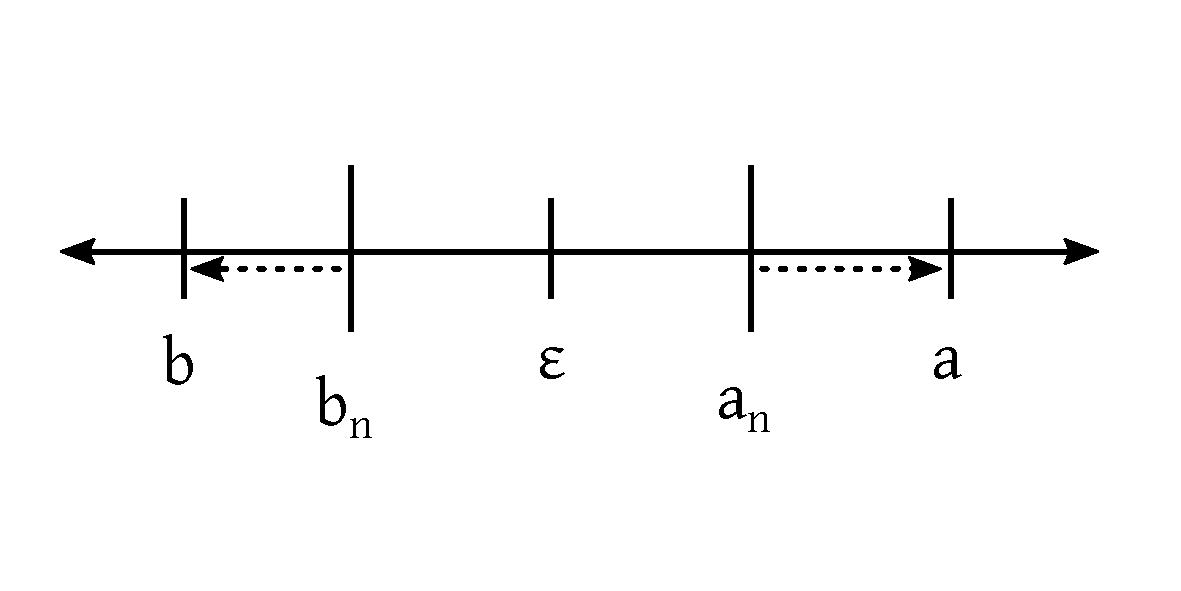
\includegraphics[width=0.3\textwidth]{img/limes.pdf}
      \caption{the sequences $a_n$, $b_n$ and limes $a$, $b$ and $\varepsilon$ in relation}
    \end{center}
  \end{figure}

  For $N = \max\set{N_1, N_2}$:
  \[
      b_N
      = b_N - b + b \leq b + \abs{b_N - b} < b \frac{\varepsilon}{2}
      = b + \frac{a - b}{2}
      = \frac12 (a + b)
  \] \[
      a_N
      = \underbrace{a_N - a}_{\geq -\abs{a_n - a}} + a \geq a - \abs{a_n - a} > a - \frac{\varepsilon}{2}
      = a - \frac{a - b}{2}
      = \frac12 (a + b)
  \] \[
      b_N < \frac12 (a + b) < d_N
  \]

  Attention:
  \[ a_n < b_n \not\Rightarrow a < b \]

  Example: $a_n = 0$, $b_n = \frac1n$.
\end{proof}

\subsection{Convergence criteria}
%
Are there criteria such that if the sequences have a specific structure,
they are obivously convergent?

\index[German]{\foreignlanguage{ngerman}{Einschließungsregel}}
\index[English]{Squeeze theorem}
\subsubsection{Squeeze theorem}
\begin{theorem}
  Let $\seq{A_n}$ and $\seq{B_n}$ be convergent real sequences with $\lim_{n \to \infty} A_n = \lim_{n \to \infty} B_n = A$.
  Let $\seq{a_n}$ be a sequence and $M \in \mathbb N$ such that
  \[ \forall n \geq M: A_n \leq a_n \leq B_n \]
  Then it holds that $\seq{a_n}$ is also convergent and $\lim{a_n} = A$.
\end{theorem}

\begin{proof}
  Let $\varepsilon > 0$ be arbitrary.
  Consider $N$ such that,
  \begin{itemize}
    \item $N \geq M$
    \item $n \geq N \Rightarrow \abs{A_n - A} < \varepsilon$
    \item $n \geq N \Rightarrow \abs{B_n - A} < \varepsilon$
  \end{itemize}
  Then it holds that for $n \geq N$:
  \[
    \left.\begin{array}{c}
      A - a_n \leq A - A_n \leq \abs{A - A_n} < \varepsilon \\
      a_n - A \leq B_n - A \leq \abs{B_n - A} < \varepsilon
    \end{array}\right\} \text{ = 1}
  \] \[
    \Rightarrow \abs{a_n - A} < \varepsilon
  \] \[
    \lim_{n \to \infty} a_N = A
  \]
\end{proof}

\begin{ex}
  Let $s \in \mathbb Q_+$. Then it holds that
  \[ \lim_{n \to \infty} \left(\sqrt[n]{n^s}\right) = 1 \]
  We apply the squeeze theorem:
  \[ n^2 \geq 1 \forall n \in \mathbb N \]
  \[ \Rightarrow \sqrt[n]{n^s} \geq 1 \]

  Let $k \in \mathbb N_+$. Then it holds that
  \[ \lim_{n \to \infty} \sqrt[n]{n^k} = \lim_{n \to \infty} \underbrace{\sqrt[n]{n} \sqrt[n]{n} \dots \sqrt[n]{n}}_{k \text { times}} \]
  \[ = 1 \cdot 1 \cdot 1 \dots = 1 \]

  For the last two lines we actually need to read them from right to left.

  Let $s = \frac pq$.
  \[ \Rightarrow n^s = n^{\frac pq} \leq q \cdot \left(n \frac{p}{q}\right)^q = n^p \]
  \[ q \geq 1 \Rightarrow \sqrt[n]{n^s}  \leq \underbrace{\sqrt[n]{n^p}}_{\text{convergent with limes }1} \qquad p \in \mathbb N \]
  Then it holds that $\lim_{n \to \infty} \sqrt[n]{n^s} = 1$ with the squeezing theorem.
\end{ex}

\begin{rem}
  Let $A \subseteq \mathbb R$ be bounded above. Then it holds that
  \[
      S = \sup{A}
      \Leftrightarrow
          s \text{ is upper bound of } A \land
          \forall \varepsilon > 0 \exists a \in A: a > s - \varepsilon
  \]
\end{rem}

\begin{proof}
  Implication from left to right:
  Let $s = \sup{A}$. Then it holds that $s$ is upper bound of $A$
  and $s - \varepsilon <  s$ is not an upper bound. Therefore $\exists a \in A: a > s - \varepsilon$.

  Implication from right to left:
  Consider that both statements on the RHS hold. So $s$ is an upper bound.
  We need to show that any $t$ is not an upper bound with $t > s$.
  Let $t < s, s - t = \varepsilon > 0$. Therefore $t = s - \varepsilon$.
  Because of the right statement $\exists a \in A: a > s - \varepsilon = t$ therefore $t$ is not an upper bound.
\end{proof}

\begin{rem}
  Analogously:
  \[ \sigma = \inf{A} \Leftrightarrow \sigma \text{ is lower bound} \land \forall \varepsilon > 0 \exists a \in A: a < \sigma + \varepsilon \]
\end{rem}

\begin{theorem}
  \label{monotonic-in-R}
  Let $(a_n)_{n \in \mathbb N}$ be a bounded monotonic sequence.
  Then $\seq{a_n}$ has a limes $a$ with
  \begin{itemize}
    \item $a = \sup\set{a_n: n \in \mathbb N}$ if $\seq{a_n}$ is monotonically increasing.
    \item $a = \inf\set{a_n: n \in \mathbb N}$ if $\seq{a_n}$ is monotonically decreasing.
  \end{itemize}
\end{theorem}

\begin{proof}
  Let $\seq{a_n}$ be monotonically increasing. Let $a = \sup\set{a_n: n \in \mathbb N}$.
  Let $\varepsilon > 0$ be arbitrary. Because $a$ is a supremum, there exists $a_N \in \set{a_n: n \in \mathbb N}$
  such that $a_N > a - \varepsilon$.
  \[ \Rightarrow \underbrace{a - a_N}_{\geq 0} < \varepsilon \]
  because $a$ is an upper bound. Therefore
  \[ \abs{a - a_N} < \varepsilon \]
  Let $n \geq N$ then it holds that
  \[ \abs{a - a_n} \underbrace{=}_{a \text{ is upper bound}} a - a_n \leq a - a_N \]
  because $a_N \leq a_n$ is increasing:
  \[ a - a_N < \varepsilon \]
  Therefore $\lim_{n \rightarrow \infty} a_n = a$.
\end{proof}

\meta{lecture}{25th of November 2015}{Wolfgang Ring}

Let $\seq{a_n}$ be a real sequence.
If $\seq{a_n}$ is bounded and monotonous.
Then $\seq{a_n} \in \mathbb N$ is convergent.

\paragraph{Example: Wallis product}

\fbox{John Wallis (1616--1703)}

\[
    p_n
    = \frac{2 \cdot 4 \cdot 6 \cdot \ldots \cdot 2n}{1 \cdot 3 \cdot 5 \dots \ldots \cdot (2n-1)}
    = \prod_{k=1}^n \frac{2k}{2k-1}
\]

Consider
\[ \alpha_n = \frac{p_n}{\sqrt{n}} \qquad \beta_n = \frac{p_n}{\sqrt{n+1}} \]

We need to show that
\begin{itemize}
  \item $(\alpha_n)$ is monotonously decreasing
  \item $(\beta_n)$ is monotonously increasing
\end{itemize}
\[ \forall n \in \mathbb N: n \geq 1: \alpha_n > \beta_n \]

Both are convergent.

\begin{enumerate}
  \item Show that,
    \[
        \alpha_{n+1} < \alpha_n \Leftrightarrow
        \frac{\alpha_{n+1}}{\alpha_n} < 1 \Leftrightarrow
        \frac{(\alpha_{n+1})^2}{(\alpha_n)^2} < 1
    \] \[
        \left(\frac{\alpha_{n+1}}{\alpha_n}\right)^2 = \left(
            \frac{\frac{2 \cdot 4 \cdot 6 \cdot \ldots \cdot (2n+2)}{1 \cdot 3 \cdot 5 \cdot \ldots \cdot (2n-1) \cdot (2n+1)}}%
            {\frac{2\cdot4\cdot \ldots \cdot 2n}{1 \cdot 3 \cdot 5 \cdot \ldots \cdot (2n+1)}}
            \cdot \frac{\frac{1}{\sqrt{n+1}}}{\frac{1}{\sqrt{n+1}}}
        \right)^2
    \] \[
        = \frac{(2n+2)^2 \cdot n}{(2n+1)^2 (n + 1)}
        = \frac{4n^3+8n^2+4n}{(4n^2 + 4n + 1)\cdot(n+1)}
        = \frac{4n^3+8n^2+4n}{4n^3+8n^2+5n+1}
        < 1
    \]
  \item We show,
    \[
        \left(\frac{\beta_{n+1}}{\beta_n}\right)^2
        = \frac{(2n+2)^2 \cdot (n+1)}{(2n+1)^2 \cdot (n+2)}
        = \frac{(4n^2 + 8n + 4) (n+1)}{(4n^2+2n+1) (n+2)}
    \] \[
        = \frac{4n^3+12n^2+12n+4}{4n^3 + 12n^2 + 9n + 2}
        > 1 \Rightarrow \beta_{n+1} > \beta_n \Rightarrow \beta_n \text{ is monotonically increasing}
    \]

    Let $p = \lim_{n\to\infty} a_n$ and $p' = \lim_{n\to\infty} b_n$.

    \[ \beta_n = \frac{p_n}{\sqrt{n}} \cdot \frac{\sqrt{n}}{\sqrt{n+1}} = \alpha_n \cdot \sqrt{\frac{n}{n+1}} \]
    \[ \lim_{n\to\infty} \beta_n = \lim_{n\to\infty} \alpha_n \sqrt{\frac{n}{n+1}} = \lim_{n\to\infty} \alpha_n \cdot \underbrace{\lim_{n\to\infty} \sqrt{\frac{n}{n+1}}}_{=1} \]
    \[ \Rightarrow \lim_{n\to\infty} \beta_n = \lim_{n\to\infty} a_n \Rightarrow p = p' \]
    It holds that $p = \lim_{n\to\infty} \frac{p_n}{\sqrt{n}} = \sqrt{n}$.
\end{enumerate}

\subsection{On limit points and subsequences}
%
\index[English]{limit point}
\index[German]{\foreignlanguage{ngerman}{Häufungspunkt}}
\begin{defi}
  Let $\seq{a_n}$ be a complex sequence.
  The complex value $a$ is called \emph{limit point} (german \enquote{\foreignlanguage{ngerman}{Häufungspunkt}})
  of $\seq{a}$ if $\forall \varepsilon > 0: \abs{a_n - a} < \varepsilon$ for infinitely many indices $n \in \mathbb N$.
  Hence infinitely many values of the sequence lie within a circle with center $a$ and radius $\varepsilon$.
\end{defi}

\begin{figure}[!t]
  \begin{center}
    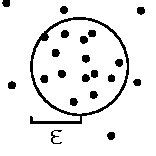
\includegraphics{img/limit_point.pdf}
    \caption{
      Illustration of a limit point in the Euclidean plane.
      The point is represented as circle with radius $\varepsilon$.
      Finitely many points lie outside the limit point; infinitely many inside.
    }
  \end{center}
\end{figure}

\begin{rem}
  Let $\seq{a_n}$ be convergent with limit $a$.
  Then it holds that $a$ is the only limit point of the sequence $\seq{a_n}$.
\end{rem}

\begin{proof}
  Let $\seq{a_n}$ be convergent. Let
  \[ \varepsilon > 0 \exists N \in \mathbb N: n \geq N \Rightarrow \abs{a_n - a} \]
  Therefore $\forall n \in \set{N, N+1, N+2, \dots}$ it holds that $\abs{a_n - a} < \varepsilon$.
  Assume $a' \in \mathbb C$ is another limit point with $a \neq a'$.
  Let
  \[ \varepsilon = \frac{\abs{a - a'}}{2} > 0 \]
  Let $N \in \mathbb N$ such that $\forall n \geq N: \abs{a_n - a} < \varepsilon$.
  \[
    \Rightarrow n \in \mathbb N: \abs{a' - a_n}
      = \abs{a' - a + a - a_n}
      = \abs{a' - a - (a_n - a)} \geq \abs{a' - a} - \abs{a_n - a}
  \] \[
      = 2\varepsilon - \abs{a_n - a} > 2\varepsilon - \varepsilon
      = \varepsilon
  \]
  At most for $n \in \set{1, \dots, N-1}$ it is possible that $\abs{a_n - a'} < \varepsilon$.
\end{proof}

\begin{rem}
  $a_n = (-1)^n$ has the limit points $+1$ and $-1$.
\end{rem}

The lecture on 26th of November 2015 got cancelled.

\meta{lecture}{27th of November 2015}{Wolfgang Ring}

\begin{defi}
  Let $a \in \mathbb C$ and $r > 0$ and
  \[ B(a, r) = \setdef{z \in \mathbb C}{\abs{z - a} < r} \]
  and we call $B(a, r)$ an \emph{open} circle with center $a$ and radius $r$.
  So the circle itself is not part of the set, unlike the following set:
  \[ B'(a, r) = \setdef{z \in \mathbb C}{\abs{z - a} \leq r} \]
\end{defi}

Let $a$ be a limit point of $\seq{a_n} \Leftrightarrow \forall \varepsilon > 0$.
$B(a, \varepsilon)$ contains infinitely many sequence values.

\begin{ex}
  \[ a_n = \frac12 \left[1 + (-1)^n \left(\frac{1-n}{n}\right)\right] \qquad n \geq 1 \]
  \[ \Rightarrow a_1 = \frac12 \quad a_2 = \frac14 \quad a_3 = \frac56 \]
  \[ a_4 = \frac18 \quad a_5 = \frac{9}{10} \quad a_6 = \frac{1}{12} \quad a_7 = \frac{13}{14} \]
  \begin{quote}
    \foreignlanguage{ngerman}{\enquote{$\frac56$? Ah, passt ma eh bessa.} (Wolfgang Ring)}
  \end{quote}

  Estimated limit points: $a = 0, b = 1$.

  \begin{proof}
    Let $\varepsilon > 0$ and $a = 0$. We consider sequence values with even index.
    So for indices it holds that $n = 2k$.
    \begin{align*}
      \abs{a_{2k} - 0}
        &= \abs{\frac12(1 + \underbrace{(-1)^{2k}}_{+1} \left(\frac{1-2k}{2k}\right))} \\
        &= \frac12 \abs{1 + \frac{1-2k}{2k}} \\
        &= \frac12 \abs{\frac{2k + 1 - 2k}{2k}} \\
        &= \frac1{4k} < \varepsilon \text{ if } \underbrace{k > \frac{1}{4\varepsilon}}_{\substack{\text{infinitely many ks} \\ \text{satisfy the relation}}}
    \end{align*}

    Let $\varepsilon > 0$ and $b = 1$. We consider sequence values of structure $n = 2k+1$.
    \begin{align*}
      \abs{a_{2k+1} - 1}
        &= \abs{\frac12 \left[1 + \underbrace{(-1)^{2k+1}}_{=-1} \left[\frac{1 - (2k+1)}{2k+1}\right]\right] - 1} \\
        &= \abs{\frac12 \left[1 - \frac{-2k}{2k+1}\right] - 1} \\
        &= \abs{\frac12 \frac{2k+1+2k}{2k+1} - 1} \\
        &= \abs{\frac{4k+1}{4k+2} - 1} \\
        &= \abs{\frac{4k+1 - 4k-2}{4k+2}} \\
        &= \frac{1}{4k+2} \\
        &< \varepsilon
    \end{align*}
    \[ \text{ if } 4k+2 > \frac1\varepsilon \Rightarrow \underbrace{k}_{\substack{\text{infinitely many} \\ \text{indices}}} > \frac14 \left(\frac1\varepsilon - 2\right) \]
  \end{proof}
\end{ex}

\begin{ex}
  $\seq{c_n}$ is defined with $c_n = i^n$.
  \[ \seq{c_n} = (1, i, -1, -i, 1, i, -1, -i, 1 \dots) \]

  What are its limit points?
\end{ex}

\index[English]{Subsequence}
\index[German]{\foreignlanguage{ngerman}{Teilfolge}}
\begin{defi}
  Let $\seq{a_n}$ with $a_n \in \mathbb C$. For example,
  \[ (1, \frac12, \frac13, \frac14, \frac15, \frac16, \dots) \]
  We remove some elements
  \[ (1, \frac13, \frac14, \frac16, \dots) \]
  A \emph{subsequence} is created.
  We also reenumerate the numbers:
  \[ (\underbrace{1}_{n_0}, \underbrace{\frac13}_{n_1}, \underbrace{\frac14}_{n_2}, \underbrace{\frac16}_{n_3}, \dots) \]
  Let $n: \mathbb N \to \mathbb N$ be strictly monotonically increasing.
  Therefore
  \[ \forall k \in \mathbb N: n (k+1) > n(k) \Rightarrow n_{k+1} > n_k \]
  We call $\seq{n_k}$ an \emph{index subsequence} and $\left(a_{n_k}\right)_{k \in \mathbb N}$ is called subsequence of $\seq{a_n}$.
\end{defi}

\begin{lemma}
  Let $\seq{a_n}$ be convergent with limes $a$ and $\left(a_{n_k}\right)_{k \in \mathbb N}$ a subsequence of $\seq{a_n}$.
  Then also the subsequence is convergent and has the same limes $a$.
\end{lemma}
\begin{proof}
  For every subsequence index $n_k$ with $k \in \mathbb N$ it holds that $n_k \geq k$.

  Proof by induction: $k=0$
  \begin{description}
    \item[$\mathbf{n_0 \in \mathbb N}$] \[ n_0 \geq 0 = k \qquad\checkmark \]
    \item[$\mathbf{n_k \geq k}$]
      Because $\underbrace{n_{k+1}}_{\in \mathbb N} > n_k$ (strictly monotonic).
      Therefore,
      \[ n_{k+1} \geq n_k + 1 > k + 1 \]
  \end{description}

  Proof of limes: $\lim_{k\to\infty} a_{n_k} = a$.
  Let $\varepsilon > 0$. Because $\seq{a_n}$ is convergent, it holds that
  $\exists N \in \mathbb N: n \geq N \Rightarrow \abs{a_n - a} < \varepsilon$.
  Let $k \geq N$. This holds because $n_k \geq k \geq N: \abs{a_{n_k} - a} < \varepsilon$.
  Therefore $\left(a_{n_k}\right)_{k \in \mathbb N}$ has limes $a$.
\end{proof}

\begin{lemma}
  Let $\seq{a_n}$ be a sequence in $\mathbb C$. Then it holds that
  $a \in \mathbb C$ is limit point if and only if there exists some subsequence
  $\left(a_{n_k}\right)_{k \in \mathbb N}$ with $\lim_{k \to \infty} a_{n_k} = a$.
\end{lemma}
\begin{proof}
  We first prove direction $\Leftarrow$.

  Assume $\left(a_{n_k}\right)_{k \in \mathbb N}$ is a convergent subsequence
  of $\seq{a_n}$ with limes $a$.
  Let $\varepsilon > 0$.
  \[ \exists N \in \mathbb N: k \geq N \Rightarrow \abs{a_{n_k} - a} < \varepsilon \]
  Therefore $B(a, \varepsilon)$ has infinitely many sequence elements of $\left(a_{n_k}\right)_{k\in\mathbb N}$
  and therefore also infinitely many sequence elements of $\seq{a_n}$.

  We prove direction $\Rightarrow$.

  We build a convergent subsequence. Consider $k \in \mathbb N$ with $k \geq 1$.
  \[ \varepsilon_k = \frac1k \]
  We define $n_0 = 0$ and $a_{n_0} = a_0$.
  Assume $a_{n_0}, a_{n_1}, \dots, a_{n_{k-1}}$ are already defined.

  Definition of $a_{n_k}$: In $B(a, \varepsilon_k)$ there are infinitely many sequence elements of $\seq{a_n}$.
  We consider $n_k > n_{k-1}$ and $a_{n_k} \in B(a, \varepsilon_k)$.

  Then it holds that $\lim_{k\to\infty} a_{n_k} = a$.
  Let $\varepsilon > 0$ be arbitrary. Consider $K > \frac1\varepsilon$.
  Hence $\varepsilon > \frac1K = \varepsilon_K$ for all $k \geq K$ it holds that
  $n_k \geq n_K$ and $\abs{a_{n_k} - a} < \varepsilon_k = \frac1k \leq \frac1K < \varepsilon$.
\end{proof}

\subsection{Bolzano-Weierstrass theorem}
\index[English]{Bolzano-Weierstrass theorem}
\index[German]{\foreignlanguage{ngerman}{Satz von Bolzano-Weierstraß}}
\fbox{Bernard Bolzano (1781--1848), Karl Weierstrass (1815--1897)}

\begin{theorem}
  Every bounded sequence of real numbers has a limit point in $\mathbb R$.
\end{theorem}
\begin{proof}
  Let $\seq{a_n}$ be a bounded sequence in $\mathbb R$, hence $\exists M > 0$
  such that all sequence elements $a_n$ in $I_0 = [-M, M]$ and let
  $F_0 = \setdef{n \in \mathbb N}{a_n \in I_0} = \mathbb N$ (index set). $F_0$ is infinite.
  We build nested intervals with the properties:
  \begin{itemize}
    \item $I_{n+1} \subseteq I_n$
    \item $\abs{I_{n+1}} = \frac12 \abs{I_n}$
    \item $F_n = \setdef{k \in \mathbb N}{a_k \in I_n}$ is infinite.
  \end{itemize}

  This construction is inductive:
  \begin{description}
    \item[induction base] $I_0 \quad \checkmark$
    \item[induction step]
      Let $I_n = [A_n, B_n]$ be given and $M_n = \frac12(A_n + B_n)$.
      Let $J_n = [A_n, M_n]$ and $L_n = [M_n, B_n]$.
      It holds that $J_n \subseteq I_n \land L_n \subseteq I_n$
      and $\card{J_n} = \frac12 \abs{I_n} \land \abs{L_n} = \frac12 \abs{I_n}$.
      Because there are infinitely many sequence elements of $\seq{a_n}$ in $I_n$
      and $I_n = J_n \cup L_n$, in at least one subinterval there have to be
      infinitely many sequence elements.

      Therefore select $I_{n+1} = J_n$ if $J_n$ contains infinitely many sequence elements
      and consider $I_{n+1} = L_n$ if $J_n$ contains only finitely many sequence elements.
      Therefore $I_{n+1}$ contains infinitely many sequence elements.
      \[ F_{n+1} = \setdef{k \in \mathbb N}{a_k \in I_{n+1}} \]
      is infinite.
      So $(I_n)_{n \in \mathbb N}$ is a nested interval.
  \end{description}

  Let $a \in \bigcap_{n \in \mathbb N} I_n$ (completeness of $\mathbb R$).

  Claim:
  $a$ is limit point of $\seq{a_n}$. Let $\varepsilon > 0$ be given and $n$ sufficiently large,
  such that $\abs{I_n} = B_n - A_n < \varepsilon$.
  Then it holds that for every $x \in I_n$ that $\abs{x - a} \leq B_n - A_n < \varepsilon$ (with $x \in I_n, a \in I_n$).
  Because $I_n$ contains infinitely many sequence elements of $\seq{a_n}$, it holds that
  infinitely many sequence elements $a_k$ satisfy the relation $\abs{a_n - a} < \varepsilon$.
  Therefore $a$ is limit point of $\seq{a_n}$.
\end{proof}

\begin{cor}[typical definition of the Bolzano-Weierstrass theorem]
  Every bounded sequence in $\mathbb R$ has a convergent subsequence.
\end{cor}

\begin{theorem}[Bolzano-Weierstrass theorem in $\mathbb C$]
  Let $\seq{a_n}$ be a bounded sequence in $\mathbb C$.
  Then $\seq{a_n}$ has a convergent subsequence and
  therefore also at least one limit point in $\mathbb C$.
\end{theorem}
\begin{proof}
  Let $\seq{a_n}$ be bounded. $a_n = \alpha_n + i \beta_n$.
  So $\seq{\alpha_n}$ is bounded in $\mathbb R$ as well as
  $\seq{\beta_n}$ is bounded in $\mathbb R$.

  Consider a convergent subsequence of $\seq{\alpha_n}$,
  $\left(\alpha_{n_k}\right)_{k \in \mathbb N}$ with
  $\lim_{k\to\infty} \alpha_{n_k} = \alpha$.
  Now consider bounded $\left(\beta_{n_k}\right)_{k \in \mathbb N}$.
  From the Bolzano-Weierstrass theorem it follows that there
  exists a convergent subsequence $\left(\beta_{n_{k_l}}\right)_{l \in \mathbb N}$
  with $\beta = \lim_{l\to\infty} \beta_{n_{k_l}}$.

  $\left(\alpha_{n_{k_l}}\right)_{l \in \mathbb N}$ is subsequence of
  $\left(\alpha_{n_k}\right)_{k \in \mathbb N}$
  convergent with limit point $\alpha$.

  Let $a_{n_{k_l}} = \alpha_{n_{k_l}} + i \beta_{n_{k_l}}$
  be a subsequence of $(a_n)_{n\in\mathbb N}$.

  Real and imaginary parts are convergent, therefore $\lim_{l\to\infty} a_{n_{k_l}} = a = \alpha + i \beta$.
  Therefore $\seq{a_n}$ contains a convergent subsequence.
\end{proof}

\meta{lecture}{2nd of December 2015}{Wolfgang Ring}
\begin{theorem}[Weierstrass-Bolzano theorem]
  Every bounded sequence in $\mathbb C$ has a convergent subsequence.
\end{theorem}

\begin{theorem}[Convergence]
  Let $(x_n)_{n \in \mathbb N}$ be convergent in $\mathbb C$ with limes $x$.
  \[ \forall \varepsilon > 0 \exists N \in \mathbb N: n \geq N: \abs{x_n - x} < \varepsilon \]
\end{theorem}

\index[English]{Distance function}
\index[German]{\foreignlanguage{ngerman}{Distanzfunktion}}
\index[English]{Metric}
\index[German]{\foreignlanguage{ngerman}{Metrik}}
\index[English]{Metric space}
\index[German]{\foreignlanguage{ngerman}{Metrischer Raum}}
\begin{defi}[Metric space]
  Let $X$ be a set. We call $d: X \times X \rightarrow \mathbb R$ a \emph{distance function} (or \emph{metric}) on $X$ if,
  \begin{itemize}
    \item $\forall x \in X: d(x, x) = 0$
    \item $\forall x,y \in X: d(x, y) = d(y, x)$ (symmetry)
    \item $\forall x,y,z \in X: d(x,z) \leq d(x,y) + d(y,z)$ (triangle inequality)
  \end{itemize}
  $(X, d)$ is called \emph{metric space}.
\end{defi}
\begin{ex}
  $X = \mathbb C$, $d(x, y) = \abs{x - y}$.
\end{ex}

\begin{defi}[Convergence with metric spaces]
  Let $X$ be a metric space. $(x_n)_{n \in \mathbb N}$ is a sequence of elements in $X$.
  Let $x \in X$. We call $\seq{x_n}$ convergent with limes $x$ if
  \[ \forall \varepsilon > 0 \exists N \in \mathbb N: n \geq N: d(x_n, x) < \varepsilon \]
\end{defi}


\index[English]{pre-compact}
\index[German]{\foreignlanguage{ngerman}{präkompakt}}
\begin{defi}
  Let $K \subseteq X$ be a subset of the metrical space $X$. We call $K$ \emph{pre-compact}
  if every sequence $\seq{a_n}$ with $a_n \in K$ has a convergent subsequence.
  $K$ is called compact if the limes $a$ of the convergent subsequence is also in $K$.
\end{defi}

\begin{defi}
  In $\mathbb C$ it holds that every bounded set is pre-compact.
\end{defi}

\subsection{Cauchy sequences in $\mathbb R$ and $\mathbb C$}
%
\fbox{Augustin-Louis Cauchy (1789--1857)}

\index[English]{Cauchy sequence}
\index[German]{\foreignlanguage{ngerman}{Cauchyfolge}}
\index[English]{Fundamental sequence}
\index[German]{\foreignlanguage{ngerman}{Fundamentalfolge}}
\begin{defi}
  Let $\seq{a_n}$ be a sequence in $\mathbb C$.
  We call $\seq{a_n}$ a \emph{Cauchy sequence} (fundamental sequence) if
  \[ \forall \varepsilon > 0 \exists N \in \mathbb N: n \geq N \land m \geq N \Rightarrow \abs{a_n - a_m} < \varepsilon \]
\end{defi}
\begin{defi}[Cauchy sequence in a metric space]
  Let $\seq{a_n}$ be a sequence in $X$.
  We call $\seq{a_n}$ a \emph{Cauchy sequence} (fundamental sequence) if
  \[ \forall \varepsilon > 0 \exists N \in \mathbb N: n \geq N \land m \geq N \Rightarrow d(a_n, a_m) < \varepsilon \]
\end{defi}

\begin{lemma}
  Every convergent sequence $\seq{a_n}$ in $\mathbb C$ is a Cauchy sequence.
\end{lemma}
\begin{proof}
  Let $\seq{a_n}$ be convergent with limes $a$.
  Let $\varepsilon > 0$ be arbitrary.

  Convergence implies that $\exists N \in \mathbb N: n \geq N \Rightarrow \abs{a_n - a} < \frac\varepsilon2$.
  For $m,n \geq N$ it holds that
  \[
      \abs{a_n - a_m}
      = \abs{a_n - a + a - a_m}
      \leq \underbrace{\abs{a_n - a}}_{< \frac\varepsilon2 \text{ because } n \geq N} + \underbrace{\abs{a - a_m}}_{< \frac\varepsilon2 \text{ because } m \geq N}
  \]
\end{proof}

\begin{lemma}
  Every Cauchy sequence $\seq{a_n}$ in $\mathbb C$ is bounded.
\end{lemma}
\begin{proof}
  Let $\seq{a_n}$ be a Cauchy sequence in $\mathbb C$.
  The Cauchy condition for $\varepsilon = 1$ states:
  \[ \exists N \in \mathbb N: \forall m,n \geq N: \abs{a_n - a_m} < 1 \]
  specifically $m = N: \forall n \geq N$
  \[ \abs{a_n - a_N} < 1 \]
  Therefore $\abs{a_n} = \abs{a_n - a_N + a_N} \leq \underbrace{\abs{a_n - a_N}}_{<1} + \abs{A_N} < \abs{a_N} + 1$.

  Let $m = \max\set{\abs{a_0}, \abs{a_1}, \dots, \abs{a_{N-1}}}$
  and $M = \max\set{m, \abs{A_N} + 1}$.

  Then for $n \leq N - 1$ it holds that
  \[ \abs{a_n} \leq m \leq M \]
  and for $n \geq N$ it holds that
  \[ \abs{a_n} \leq \abs{a_N} + 1 \leq M \]
  Therefore $\forall n \in \mathbb N: \abs{a_n} \leq M$.
  Therefore $\seq{a_n}$ is bounded.
\end{proof}

\subsection{Is $\mathbb C$, $\mathbb R$ and $\mathbb Q$ complete?}
%
\index[English]{Completeness of $\mathbb C$}
\index[German]{\foreignlanguage{ngerman}{Vollständigkeit von $\mathbb C$}}
\begin{theorem}[Cauchy sequences and limes]
  Every Cauchy sequence in $\mathbb C$ has a limes and is therefore convergent.
  Followingly we call $\mathbb C$ to be \emph{complete}.
\end{theorem}
\begin{proof}
  Let $\seq{a_n}$ be a Cauchy sequence in $\mathbb C$.
  We know that $\seq{a_n}$ is bounded.
  From the Bolzano-Weierstrass theorem it follows that a limit point $a$
  of $\seq{a_n}$ exists. Let $\varepsilon > 0$ be arbitrary.
  \begin{enumerate}
    \item We choose $N \leq \mathbb N$ sufficiently large such that
      \[ n,m \geq N \Rightarrow \abs{a_n - a_m} < \frac\varepsilon2 \]
    \item Because $B(a, \frac\varepsilon2)$ contains infinitely many sequence elements ($a$ is limit point),
      $K \geq N$ exists with $\abs{a - a_K} < \frac{\varepsilon}{2}$.
  \end{enumerate}
  Let $n \geq N$. Then
  \[
      \abs{a_n - a}
      = \abs{a_n - a_K + a_K - a} \leq \underbrace{\abs{a_n - a_K}}_{< \frac\varepsilon2 \text{ (Cauchy seq.)}} + \underbrace{\abs{a_K - a}}_{< \frac\varepsilon2 \text{ (limit point $a$)}}
      < \frac\varepsilon2 + \frac\varepsilon2 = \varepsilon
  \]
  Therefore $\seq{a_n}$ is convergent with limes $a$.

  We have proven that if $\seq{a_n}$ has a limit point, this limit point is also its limes.

  We concluded: nested intervals $\Rightarrow$ compactness / Bolzano-Weierstrass theorem $\Rightarrow$ completeness.

  Actually nested intervals are equivalent to completeness.
\end{proof}

\meta{lecture}{3rd of December 2015}{Wolfgang Ring}

\begin{cor}
  $\mathbb C$ is complete.
\end{cor}
\begin{proof}
  Let $\seq{z_n}$ be a Cauchy sequence in $\mathbb C$.
  \[ z_n = a_n + i b_n \]
  Then $\seq{a_n}$ and $\seq{b_n}$ are Cauchy sequences in $\mathbb R$.

  Show that this property: Let $\varepsilon > 0$. Because $\seq{z_n}$ is a Cauchy sequence,
  it holds that
  \[ \exists N \in \mathbb N: n,m \geq N \Rightarrow \abs{z_n - z_m} < \varepsilon \]
  Because $\abs{a_n - a_m} \leq \abs{z_n - z_m}$ and $\abs{b_n - b_m} \leq \abs{z_n - z_m}$ hold,
  it follows that for $n,m \geq N: \abs{a_n - a_m} < \varepsilon \land \abs{b_n - b_m} < \varepsilon$.
  Therefore $\seq{a_n}$ and $\seq{b_n}$ are Cauchy sequences.

  Because $\mathbb R$ is complete, it follows that $\exists a \in \mathbb R$ such that
  \[ a = \lim_{n\to\infty} a_n \text{ and } \exists b \in \mathbb R \]
  with $b = \lim_{n\to\infty} b_n$. Because $\lim_{n\to\infty} z_n = z = a + ib$,
  \[ \Leftrightarrow a = \lim_{n\to\infty} a_n \land b = \lim_{n\to\infty} b_n \]
\end{proof}

\begin{ex}
  We show a counterexample for the completeness of $\mathbb Q$.
  So we have Cauchy sequences with limes, which lies outside $\mathbb Q$.

  We define a recursion:
  \[
    a_n = \begin{cases}
      2 & \text{if } n = 0 \\
      \frac12 \left(a_n + \frac2{a_n}\right) & \text{if } n > 0
    \end{cases}
  \]
  We observe, $\forall n \in \mathbb N: a_n > 0 \land a_n \in \mathbb Q$.

  Proof by complete induction:
  \begin{description}
    \item[Induction base: $n = 0$]
      \[ a_0 = 2 > 0 \land 2 \in \mathbb Q \quad \checkmark \]
    \item[Induction step: $n \rightarrow n + 1$]
      Let $a_n > 0$ and $a_n \in \mathbb Q$.
      \[ a_{n+1} = \frac12 \left(\underbrace{a_n}_{>0} + \underbrace{\frac2{a_n}}_{>0}\right) > 0 \]
      and $a_{n+1} \in \mathbb Q$.
  \end{description}

  We prove by induction: $\forall n \in \mathbb N: a_n^2 > 2$.
  \begin{description}
    \item[Induction base: $n = 0$]
      \[ a_0 = 2 \qquad a_0^2 = 4 > 2 \quad \checkmark \]
    \item[Induction step: $n \rightarrow n+1$]
      It holds that $a_n^2 - 2 > 0$.
      \[
          a_{n+1}^2 - 2
          = \frac14 \left(a_n^2 + 4 + \frac4{a_n^2}\right) - 2
          = \frac{1}{4a_n^2} \left(a_n^4 + 4a_n^2 + 4 - 8a_n^2\right)
      \] \[
          = \frac{1}{4a_n^2} \left(a_n^4 - 4a_n^2 + 4\right)
          = \frac{1}{4a_n^2} \underbrace{\left(a_n^2 - 2\right)^2}_{>0} > 0
      \]
  \end{description}

  Furthermore it holds that $a_{n+1} < a_n$.
  \[ 2a_{n+1} = a_n + \frac2{a_n} \Rightarrow 2 (a_{n+1} - a_n) = -a_n + \frac2{a_n} = \frac{\overbrace{2 - a_n^2}^{<0}}{a_n} < 0 \]
  \[ \Rightarrow a_{n+1} - a_n < 0 \Rightarrow a_{n+1} < a_n \]

  Therefore the sequence $\seq{a_n}$ is strictly monotonically decreasing and is bound by below.
  Therefore some $a \in \mathbb R$ exists with $a = \lim_{n\to\infty} a_n$.

  Monotonicity really depends on the completeness of $\mathbb R$.
  We cannot argue equivalently to Theorem~\ref{monotonic-in-R} with the supremum.

  For this example we know that $\seq{a_n}$ is convergent in $\mathbb R$.
  $\seq{a_n}$ is Cauchy sequence in $\mathbb R$.
  So $\seq{a_n}$ is Cauchy sequence in $\mathbb Q$.

  For the limes $a$ it holds that,
  \[ a = \lim_{n\to\infty} a_{n+1} = \lim_{n\to\infty} \frac12 \left(a_n + \frac{2}{a_n}\right) \]
  \[ = \frac12 \lim_{n\to\infty} a_n + \frac12 \frac{2}{\lim_{n\to\infty} a_n} = \frac12 a + \frac1a \]

  \[ a = \frac12 a + \frac1a \Rightarrow \frac12 a = \frac1a \]
  \[ a^2 = 2 \Rightarrow a = +\sqrt{2} \not\in \mathbb Q \]

  Therefore $\seq{a_n}$ is \emph{not} convergent in $\mathbb Q$.
  We found a convergent Cauchy sequence whose limes is not in $\mathbb Q$ which
  immediately means that $\mathbb Q$ is incomplete.
\end{ex}

\index[English]{Tending towards infinity}
\index[German]{\foreignlanguage{ngerman}{Uneigentliche Grenzwerte}}
\begin{defi}[Tending towards infinity]
  Let $\seq{a_n}$ be a sequence of real numbers.
  \begin{itemize}
    \item
      We state $\seq{a_n}$ \emph{tends to infinity} with limes $+\infty$:
      \[ \lim_{n\to\infty} a_n = +\infty \]
      \[ \text{if } \forall M > 0 \exists N \in \mathbb N: n \geq N \Rightarrow a_n > M \]
    \item
      We state $\seq{a_n}$ \emph{tends to negative infinity} with limes $-\infty$:
      \[ \lim_{n\to\infty} a_n = -\infty \]
      \[ \forall M > 0 \exists N \in \mathbb N: n \geq N \Rightarrow a_n < -M \]
  \end{itemize}
\end{defi}
\begin{ex}
  \[ a_n = \frac{n^2 + 2}{n+1} \]
  has limes $+\infty$.
  The proof is given in the practicals. We show that \dots
  \[ \frac{n^2 + 2}{n + 1} > M \Leftrightarrow \dots \]
\end{ex}

\index[English]{Limes superior}
\index[German]{\foreignlanguage{ngerman}{Limes superior}}
\index[English]{Limes inferior}
\index[German]{\foreignlanguage{ngerman}{Limes inferior}}
\begin{defi}[Limes superior, Limes inferior]
  Let $\seq{a_n}$ be a real sequence which is bounded above and
  \[ H = \setdef{\xi \in \mathbb R}{\xi \text{ is limit point of } \seq{a_n}} \neq \emptyset \]

  Then $H$ is also bounded by above and we call $S^* = \sup{H}$ a \emph{limes superior}
  of the sequence $\seq{a_n}$. We denote:
  \[ S^* = \limsup_{n\to\infty} a_n \]

  Let $\seq{a_n}$ be a real sequence which is bounded below and
  \[ H = \setdef{\xi \in \mathbb R}{\xi \text{ is limit point of } \seq{a_n}} \neq \emptyset \]

  Then $H$ is also bounded by below and we call $S^* = \inf{H}$ a \emph{limes inferior}
  of the sequence $\seq{a_n}$. We denote:
  \[ S_* = \liminf_{n\to\infty} a_n \]
\end{defi}

\begin{theorem}
  If $\seq{a_n}$ is bounded by above by $M$, $H \neq \emptyset$, then $M$ is also an upper bound of $H$.
\end{theorem}
\begin{proof}
  Assume $\exists s \in H$ with $s > M$. Choose $\varepsilon = S - M > 0$.
  Because $S$ is a limit point of $\seq{a_n}$ it holds that $(s - \varepsilon, s + \varepsilon)$
  contains infinitely many sequence elements. So for infinitely many indices $n$ it holds that,
  \[ a_n > s - \varepsilon = s - (s - M) = M \]
  This contradicts with $M$ being the upper bound of the sequence.
\end{proof}

\begin{lemma}
  Let $\seq{a_n}$ be bounded by above. $a_n \in \mathbb R$. Let $H \neq \emptyset$ be defined as above.
  Then it holds that
  \[ S^* = \limsup_{n\to\infty}(a_n) = \max H \]
  ie. $S^*$ is a limit point itself of the sequence.
\end{lemma}
\begin{proof}
  Show that $S^*$ itself is a limit point of the sequence.
  Let $\varepsilon > 0$: Choose $\xi \in H$ such that
  \[ \xi > S^* - \frac\varepsilon2 \Rightarrow S^* - \xi = \abs{S^* - \xi} < \frac\varepsilon2 \]
  Because $\xi$ is a limit point of the sequence, in $(\xi - \frac\varepsilon2, \xi + \frac\varepsilon2)$
  there are infinitely many sequence elements.

  Let $x \in (\xi - \frac\varepsilon2, \xi + \frac\varepsilon2) \Leftrightarrow \abs{x - \xi} < \frac\varepsilon2$.
  Then it holds that
  \[
      \abs{x - S^*}
      = \abs{x - \xi + \xi - S^*}
      \leq \underbrace{\abs{x - \xi}}_{< \frac\varepsilon2} + \underbrace{\abs{\xi - S^*}}_{= S^* - \xi < \frac\varepsilon2}
  \] \[
      \Rightarrow x \in (S^* - \varepsilon, S^* + \varepsilon)
  \]
  Followingly,
  \[
    \underbrace{\left(\xi - \frac\varepsilon2, \xi + \frac\varepsilon2\right)}%
      _{\substack{\text{contains infinitely many} \\ \text{sequence elements}}}
    \subseteq \underbrace{\left(S^* - \varepsilon, S^* + \varepsilon\right)}%
      _{\substack{\text{contains infinitely many} \\ \text{sequence elements}}}.
  \]
\end{proof}

\begin{rem}
  The analogous statement holds for the limes inferior.
  \[ S^* = \limsup_{n\to\infty} a_n \Leftrightarrow \]
  \begin{enumerate}
    \item $S^* \in H$, therefore $S^*$ is limit point of $\seq{a_n}$.
    \item $\forall \varepsilon > 0 \exists N \in \mathbb N: n \geq N: a_n < S^* + \varepsilon$
  \end{enumerate}
\end{rem}

\begin{proof}
  Let $S^* = \limsup_{n\to\infty} a_n$.
  \begin{enumerate}
    \item The first property holds immediately.
    \item
      We use an indirect proof.
      \[ \Rightarrow \exists \varepsilon > 0: \forall N \in \mathbb N: \exists n \geq N: a_n \geq S^* + \varepsilon \]
      Therefore infinitely many sequence elements $a_n$ exist with $a_n \geq S^* + \varepsilon$.
      We sort the sequence elements in a subsequence $\left(a_{n_k}\right)_{k \in \mathbb N}$.
      It holds that
      \[ S^* + \varepsilon \leq a_{n_k} \leq M \]
      $\left(a_{n_k}\right)_{k \in \mathbb N}$ is bounded and has a limit point $S$
      with $S^* + \varepsilon < S \Rightarrow S > S^*$.
      $S$ is also a limit point of the original sequence $\seq{a_n}$ with $S > S^* = \max{H}$.
      This is a contradiction.
  \end{enumerate}
\end{proof}


\meta{lecture}{9th of December 2015}{Wolfgang Ring}
\begin{theorem}[Repetition of the theorem]
  Let $\seq{a_n}$ be bounded above and let $\seq{a_n}$ has a limit point.
  Then it holds that $S^* = \limsup_{n\to\infty} a_n \Leftrightarrow$
  \begin{enumerate}
    \item $S^*$ is limit point of $\seq{a_n}$.
    \item $\forall \varepsilon > 0 \exists N \in \mathbb N: n \geq N: a_n < S^* + \varepsilon$
  \end{enumerate}
  Therefore above $S^* + \varepsilon$ there are only finitely many sequence elements.
\end{theorem}
\begin{proof}
  We prove the first direction $\Rightarrow$.

  Let $S^* = \limsup_{n\to\infty} a_n$. Let $\varepsilon > 0$ be arbitrary.
  The first property follows immediately.
  The second property needs to be shown.

  \begin{proof}[Proof by contradiction for the second property]
    \[ \exists \varepsilon > 0 \forall N \in \mathbb N: \exists n \geq N: a_n \geq S^* + \varepsilon \]
    Then we build a subsequence $\left(a_{n_k}\right)_{k\in\mathbb N}$ from $\seq{a_n}$ with $a_{n_k} \geq S^* + \varepsilon$.

    The subsequence is built inductively:
    \begin{description}
      \item[$n = 0$]
        then (because the second property holds negated) there exists $x_n \geq 0: a_{n_0} \geq S^* + \varepsilon$.
      \item[$k \to k+1$]
        Let $a_{n_0}, a_{n_1}, \dots, a_{n_k}$ be found with $a_{n_l} \geq S^* + \varepsilon$ with $l = 0, \dots, n$
        and $n_l < n_{l+1}$. Let $N = n_k + 1$. Because the second property holds negated, $n_{k+1} \geq N > n_k$
        such that $a_{n_{k+1}} \geq S^* + \varepsilon$.
    \end{description}

    The subsequence's elements have the properties:
    \begin{itemize}
      \item $a_{n_k} \geq S^* + \varepsilon \qquad \forall k \in \mathbb N$
      \item Because $\seq{a_n}$ is bounded above, also $\left(a_{n_k}\right)_{k\in\mathbb N}$ is bounded above
    \end{itemize}
    From the Bolzano-Weierstrass theorem it follows that $\left(a_{n_k}\right)_{k\in\mathbb N}$ has a limit point
    $S \geq S^* + \varepsilon$. Because every limit point of $\left(a_{n_k}\right)_{k\in\mathbb N}$ is a limit point
    of $\seq{a_n}$, it holds that $S$ is limit point of $\seq{a_n}$ and $S > S^* + \varepsilon > S^*$.
    This is a contradiction.
  \end{proof}

  We prove the second direction $\Leftarrow$.

  Assume properties 1 and 2 hold. It remains to show that $S^*$ is the largest limit point.
  Assume $S > S^*$. We need to show that $S$ cannot be a limit point.

  \[
    \varepsilon = \frac{S - S^*}{2} > 0
    \Rightarrow 2\varepsilon = S - S^*
    \Rightarrow S^* + \varepsilon = S - \varepsilon
  \]
  Because the second property holds, there exists some $N \in \mathbb N$ such that
  $\forall n \geq N \Rightarrow a_n < S^* + \varepsilon$. Therefore only finitely many
  sequence elements are larger than $S^* + \varepsilon = S - \varepsilon$.
  Therefore at most finitely many sequence elements $(S - \varepsilon, S + \varepsilon)$.
  Followingly $S$ is not a limit point.
\end{proof}

\begin{theorem}[Analogous result for limes inferior]
  \[ S_* = \liminf_{n\to\infty} a_n \Leftrightarrow \]
  \begin{enumerate}
    \item $S_*$ is limit point of $\seq{a_n}$.
    \item $\forall \varepsilon > 0 \exists N \in \mathbb N: n \geq N: a_n > S_* - \varepsilon$
  \end{enumerate}
\end{theorem}

\begin{theorem}
  Let $\seq{a_n}$ be bounded above and $\seq{a_n}$ has a limit point.
  \begin{itemize}
    \item Let $k \in \mathbb N$. We define
      \[ A_k = \set{a_k, a_{k+1}, a_{k+2}, \dots} = \set{a_j: j \geq k} \]
    \item It holds that $A_{k+1} \subseteq A_k$ and $A_k$ is bounded above\footnote{Obviously.}.
  \end{itemize}
  We define $S_k = \sup{A_k}$. Then $\left(S_k\right)_{k\in\mathbb N}$ is a monotonically decreasing
  sequence in $\mathbb R$ and $\left(S_k\right)_{k\in\mathbb N}$ is bounded below.
  Therefore $\left(S_k\right)_{k\in\mathbb N}$ is convergent and it holds that
  \[ \lim_{n\to\infty} S_k = \inf\set{S_k: k \in \mathbb N} = S^* \]
  It turns out that
  \[ S^* = \limsup_{n\to\infty} a_n \]
  We denote
  \[
      \lim_{k\to\infty} \sup{A_k}
      = \lim_{k\to\infty} \sup \set{a_j: j \geq k}
      = \inf\set{\sup{A_k}: k \in \mathbb N}
      = \limsup_{n\to\infty} a_n
  \]
\end{theorem}
\begin{proof}
  \[ A_{k+1} \subseteq A_k \Rightarrow \sup{A_{k+1}} \leq \sup{A_{k}} \Rightarrow S_{k+1} \leq S_k \]
  $\left(S_k\right)_{k\in\mathbb N}$ is bounded below. Choose
  $\xi \in H$ and $\xi$ is limit point of $\seq{a_n}$.
  Then $\xi - 1$ is a lower bound for $\left(S_k\right)_{k\in\mathbb N}$ because infinitely many sequence elements
  are in $(\xi - 1, \xi + 1)$.
  Therefore,
  \[
    \forall k \in \mathbb N: \exists n \geq k: a_n > \xi - 1
    \quad\Rightarrow S_k = \sup{A_k} > \xi - 1
    \quad\checkmark
  \]
  We know that $\left(S_k\right)_{k\in\mathbb N}$ is convergent. Let $S^* = \lim_{n\to\infty} S_k$.
  We show the first property:

  $S^*$ is limit point of $\left(a_n\right)_{n\in\mathbb N}$.
  Let $\varepsilon > 0$ be given. We need to show that infinitely many sequence elements
  are in $(S^* - \varepsilon, S^* + \varepsilon)$.

  Because $\lim_{k\to\infty} S_k = S^*$ there exists some
  \[ N \in \mathbb N: k \geq N \Rightarrow \underbrace{\abs{S_k - S^*}}_{-S^*} < \frac\varepsilon2. \]
  We build a subsequence of $\seq{a_n}$ inductively, which is entirely inside $(S^* - \varepsilon, S^* + \varepsilon)$.
  Because $S_N = \sup\set{a_N, a_{N+1}, a_{N+2}, \dots}$ exists, there exists $a_j \geq S_N - \frac\varepsilon2$ with $j \geq N$.
  \[ \Rightarrow \underbrace{S_N - a_j}_{=\abs{S_N - a_j}} \leq \frac\varepsilon2 \]
  \begin{description}
    \item[$k = 0$]
      Choose $n_0 = j \geq N$ ($j$ from above), therefore it holds that
      \[
        \abs{S^* - a_{n_0}} = \abs{S^* - S_N + S_N - a_{n_0}} \leq \abs{S^* - S_N} + \abs{S_N - a_j}
      \] \[
        < \frac\varepsilon2 + \frac\varepsilon2
        = \varepsilon
      \]
      Therefore $a_{n_0} \in (S^* - \varepsilon, S^* + \varepsilon)$.
    \item[$k \to k+1$]
      Consider $a_{n_0}, a_{n_1}, \dots, a_{n_k}$ such that $n_k > n_{k-1} > \dots > n_0 \geq N$ holds
      and $\abs{a_{n_l} - S^*} < \varepsilon$. Because $n_k + 1 > N$ holds
      \[ \abs{S^* - S_{n_k + 1}} < \frac\varepsilon2 \]
      because $S_{n_k + 1} = \sup\set{a_{n_k + 1}, a_{n_k + 2}, \dots}$,
      exists ${j'} \geq n_k + 1 > n_k$ such that
      \[ \abs{S_{n_k + 1} - a_{j'}} = S_{n_k + 1} - a_{j'} < \frac\varepsilon2 \]
      Choose $n_{k+1} = {j'}$ from above.
      \[ n_{k+1} \geq n_k + 1 > n_k \text{ and } \abs{S^* - a_{n_{k+1}}} = \abs{S^* - S_{n_k + 1} + S_{n_k + 1} - a_{j'}} \]
      \[ \leq \abs{S^* - S_{n_k + 1}} + \abs{S_{n_k + 1} - a_{j}} < \frac\varepsilon2 + \frac\varepsilon21 = \varepsilon \]
      Therefore we have found a subsequence $\left(a_n\right)_{n\in\mathbb N}$ such that
      \[ \forall k \in \mathbb N: a_{n_k} \in (S^* - \varepsilon, S^* + \varepsilon) \]
      $\Rightarrow S^*$ is limit point of the sequence.

      We show that $S^*$ is the largest limit point.
      Let $S < S^*$. We show that $S$ is not a limit point.

      Let $\varepsilon = \frac12(S - S^*) > 0$ such that $S^* + \varepsilon = S - \varepsilon$.
      Choose $k \in \mathbb N$ such that $S_k - S^* = \abs{S_k - S^*} < \varepsilon$.
      $\forall n \geq K$ it holds that $a_n \leq S_k < S^* + \varepsilon = S - \varepsilon$.
      Therefore there are at most finitely many sequence elements in $(S - \varepsilon, S + \varepsilon)$.
      Therefore $S$ is not a limit point.
  \end{description}
\end{proof}

The analogous result for the limes inferior also holds and is given in the practicals.

\section{Infinite series}
\index[English]{Series}
\index[German]{\foreignlanguage{ngerman}{Reihen}}
\index[English]{Infinite series}
\index[German]{\foreignlanguage{ngerman}{Unendliche Reihen}}
\index[English]{Partial sum}
\index[German]{\foreignlanguage{ngerman}{Partialsumme}}
\index[English]{n-th partial sum}
\index[German]{\foreignlanguage{ngerman}{n-te Partialsumme}}
\index[English]{Convergent series}
\index[German]{\foreignlanguage{ngerman}{Konvergente Reihe}}
\begin{defi}
  Let $\seq{a_n}$ be a sequence of complex values. We define
  \begin{itemize}
    \item $S_0 = a_0$
    \item $S_1 = a_0 + a_1$
    \item $S_2 = a_0 + a_1 + a_2$
    \item $\dots$
    \item $S_n = a_0 + a_1 + \dots + a_n = \sum_{k=0}^n a_k$
  \end{itemize}
  We call $\seq{S_n}$ an \emph{infinite series} with $a_k$ sequence elements.
  We call $S_n$ the \emph{n-th partial sum} of the series.
  The series is called \emph{convergent} if $\seq{S_n}$ is a convergent series in $\mathbb C$.
  For a convergent series instead of
  \[ S = \lim_{n\to\infty} S_n = \lim_{n\to\infty} \underbrace{\sum_{k=0}^n a_k}_{= S_n} \]
  we denote
  \[ S = \sum_{k = 0}^\infty a_k \]
  Actually a series must be denoted like a sequence with $\seq{S_n}$.
  But we also say \enquote{let $\sum_{k=0}^\infty a_k$ be a series}
  (but actually the sum of partial sums is meant).
  So this an ambiguous definition (per default always assume that the sum of partial sums is considered).
\end{defi}

\subsection{The geometric series}
\index[English]{Geometric series}
\index[German]{\foreignlanguage{ngerman}{Geometrische Reihe}}
\begin{theorem}
  Let $q \in \mathbb C$ with $q \neq 1$.
  Consider $\sum_{k=0}^\infty q^k$ hence $S_n = \sum_{k=0}^{n} q^n$.
  The limes of this series is given with $\frac{1 - q^{n+1}}{1 - q}$ for $\abs{q} < 0$.
  % TODO: \abs{q} < 0    makes no sense, bc \abs{q} \geq 0 for all q?!
\end{theorem}
\begin{proof}
  We find a simple equation for $S_n$:
  \[ S_n - q \cdot S_n = (1 - q) S_n \]
  \[ (1 + q + q^2 + \dots + q^n) - q (1 + q + q^2 + \dots + q^n) \]
  \[ = (1 + q + q^2 + \dots + q^n) - (q + q^2 + \dots + q^n + q^{n+1}) \]
  \[ = (1 - q^{n+1}) \]
  Therefore $(1 - q) \cdot S_n = 1 - q^{n+1}$. That is,
  \[ S_n = \frac{1 - q^{n+1}}{1 - q} \]

  If $\abs{q} < 1$ it holds that
  \[ \lim_{n\to\infty} q^{n+1} = q \lim_{n\to\infty} q^n = q \cdot 0 = 0 \]
  \[ \lim_{n\to\infty} S_n = \frac{1 - \lim_{n\to\infty} q^{n+1}}{1 - q} = \frac{1}{1 - q} \]
  \[ \sum_{k=0}^\infty q^k = \frac{1}{1 - q} \]

  If $\abs{q} > 1$ it holds that
  \[
    \abs{S_n}
    = \frac{1}{\abs{1 - q}} \cdot \abs{1 - q^{n+1}}
    \geq \frac{1}{\abs{1 - q}} \left(\abs{q^{n+1}} - 1\right)
  \]
  This is the inversed triangle inequality.
  \[ = \frac{1}{\abs{1 - q}} \left(\underbrace{\abs{q}^{n+1}}_{\to\infty} - 1\right) \]
  Hence $\seq{S_n}$ is unbounded and therefore not convergent.
\end{proof}

\index[English]{Harmonic series}
\index[German]{\foreignlanguage{ngerman}{Harmonische Reihe}}
\begin{theorem}
  Let $a_n = \frac1n$ hence $\sum_{k=1}^\infty \frac1k$.
  \[ \sum_{k=1}^\infty \frac1n \text{ is divergent} \]
\end{theorem}
\begin{proof}
  Consider
  \[ \sum_{k=1}^\infty \frac1n = 1 + \frac12 + \frac13 + \frac14 + \frac15 + \frac16 + \frac17 + \frac18 + \dots \]
  \[ > \frac12 + \frac12 + \frac12 + \frac14 + \frac14 + \frac16 + \frac16 + \frac18 + \frac18 + \dots \]
  \[ = \frac12 + 2 \left(\frac12 + \frac14 + \frac16 + \frac18 + \frac1{10} + \dots\right) \]
  \[ = \frac12 + 2 \frac12 \left(1 + \frac12 + \frac13 + \frac14 + \frac15 + \dots\right) \]
  \[ = \frac12 + \left(1 + \frac12 + \frac13 + \frac14 + \frac15 + \dots\right) \]
  \[ = \frac12 + \sum_{k=1}^\infty \frac1n \]
  So we have,
  \[ \sum_{k=1}^\infty \frac1n > \frac12 + \sum_{k=1}^\infty \frac1n \]
  Let $\sum_{k=1}^\infty \frac1n = H$, then $H > \frac12 + H$ must hold for some real value.
  This is impossible, so $H$ cannot exist. Hence $\sum_{k=1}^\infty \frac1n$ diverges.
\end{proof}

\meta{lecture}{9th of December 2015}{Wolfgang Ring}

TODO

\begin{description}
  \item[Case 1]
    \[ n = 2^k - 1 \]
    \[ S_{\alpha,2^1-1} = \underbrace{1}_{<\frac{1}{2^\alpha}} + \underbrace{\frac1{2^\alpha} + \frac{1}{3^\alpha}}_{2^1 \text{ terms}} + \underbrace{\frac{1}{4^\alpha} + \frac{1}{5^\alpha} + \frac{1}{6^\alpha} + \frac{1}{7^\alpha}}_{2^2 \text{ terms}} \]
    \[ + \underbrace{\frac1{8^\alpha} + \dots}_{2^3 \text{ terms}} TODO \]

    \[ < 1 + 2 \frac{1}{2^\alpha} + 4 \frac{1}{4^\alpha} + 8 \frac{1}{8^\alpha} + \dots + 2^{k-1} \frac{1}{\left(2^{k-1}\right)^\alpha} \]
    \[ = 1 + \frac{1}{2^{\alpha-1}} + \frac{1}{4^{\alpha-1}} + \frac{1}{8^{\alpha-1}} + \dots + \frac{1}{\left(2^{n-1}\right)^{\alpha-1}} \]
    \[ = 1 + \frac{1}{2^{\alpha-1}} + \left(\frac{1}{2^{\alpha-1}}\right)^2 + \left(\frac{1}{3^{\alpha-1}}\right)^3 + \dots \]
    \[
      = \underbrace{\sum_{j=0}^{k-1} \left(\frac{1}{2^{\alpha-1}}\right)^2}_{\substack{\text{geometric} \\ \text{series}}}
      = \frac{1 - \left(\frac{1}{2^{\alpha-1}}\right)^2}{1 - \frac1{2^{\alpha-1}}}
    \]

    Therefore $(S_{\alpha,2^k-1})$ is bounded.
    Let $n \in \mathbb N$ be arbitrary and choose a sufficiently large $K$ such that $2^k > n+1$. Therefore $2^k-1 > n$.
    Because $\frac{1}{j^\alpha} > 0$ for all $j \geq 1$, it holds that $S_{2^k-1} > S_n$.
    At the same time $S_{2^k-1} < \frac{2^{\alpha-1}}{2^{\alpha-1}-1}$. So $\seq{S_n}$ is bounded.
    Hence $\sum_{k=1}^\infty \frac{1}{k^\alpha}$ is convergent.
  \item[Case 2: $\mathbf{\alpha \leq 1}$]
    Then it holds that $k^\alpha \leq k$ and therefore $\frac{1}{k^\alpha} \geq \frac1{k}$.
    Because $S_{\alpha,n} \geq S_{1,n}$ and because $S_{1,n}$ is unbounded, it holds that
    $\seq{S_{\alpha,n}}$ is unbounded and followingly $\sum_{k=0}^\infty \frac1{k^\alpha}$ is divergent.
\end{description}

\index{Riemann's zeta function}
\index{\foreignlanguage{ngerman}{Riemannsche Zeta-Funktion}}
\begin{rem}
  $\alpha \in \mathbb Q_+$ can be replaced by $\alpha \in \mathbb R_+$.
  It is even possible to choose $\alpha \in \mathbb C$.
  Then we can define $\zeta: M \subseteq \mathbb C \rightarrow \mathbb C$
  with $\xi(z) = \sum_{k=1}^\infty \frac{1}{k^z}$.
  This is Riemann's Zeta function.
\end{rem}

\index{Alternating sequence}
\index{\foreignlanguage{ngerman}{Alternierende Folge}}
\index{Alternating series}
\index{\foreignlanguage{ngerman}{Alternierende Reihe}}
\begin{defi}
  Let $\seq{a_n}$ be a real sequence with $a_n \geq 0$.
  Then we call $\seq{\alpha_n}$ with $\alpha_n = (-1)^n a_n$, or equivalently
  $\alpha_n = (-1)^{n+1} a_n$, an \index{alternating sequence}.

  A series of structure $\sum_{k=0}^\infty (-1)^k a_k$ with $a_k \geq 0$
  is called \emph{alternating series}.
\end{defi}

\subsection{Leibniz convergence criterion}
\fbox{\foreignlanguage{ngerman}{Gottfried Wilhelm Leibniz (1646--1716)}}
\index{Leibniz convergence criterion}
\index{\foreignlanguage{ngerman}{Leibniz' Konvergenzkriterium}}
\index{\foreignlanguage{ngerman}{Konvergenzkriterium von Leibniz}}
\begin{theorem}[Leibniz convergence criterion]
  Let $\seq{a_n}$ be a real, monotonically zero sequence with $a_n \geq a_{n+1} \geq 0
  \quad\forall n \in \mathbb N$.
  Then $\sum_{k=0}^\infty (-1)^k a_k$ is convergent.
\end{theorem}
\begin{proof}
  \begin{align*}
    S_{2n-1} &= \sum_{k=0}^{2n-1} (-1)^{k} a_k \\
    S_{2n} &= \sum_{k=0}^{2n-1} (-1)^{k} a_k + (-1)^{2n} a_{2n} \\
      &= S_{2n-1} + a_{2n} \\
    S_{2n+1} &= S_{2n-1} + \underbrace{a_{2n} - a_{2n-1}}_{\geq 0} \\
    S_{2n+2} &= \underbrace{S_{2n-1} + a_{2n}}_{S_{2n}} \underbrace{- a_{2n+1} + a_{2n+2}}_{= -(a_{2n+1} - a_{2n+2}) \geq 0}
  \end{align*}
  Therefore it holds that $S_{2n+1} \geq S_{2n-1}$, $S_{2n+2} \leq S_{2n}$ and $S_{2n} \geq S_{2n-1}$.

  $\seq{S_{2n}}$ is monotonically decreasing.
  $\seq{S_{2n+1}}$ is monotonically increasing.

  It holds that: $\forall m,n \in \mathbb N: S_{2n} \geq S_{2m - 1}$.

  \begin{proof}
    \begin{description}
      \item[Case 1: $\mathbf{m > n}$]
        \[ S_{2m+1} \leq S_{2n} \leq S_{2n} \qquad\checkmark \]
      \item[Case 2: $\mathbf{m \leq n}$]
        \[ S_{2m+1} \leq S_{2n+1} \underbrace{\leq}_{\alpha < 1} S_{2n} \]
    \end{description}
    So $\seq{S_{2n}}$ is monotonically decreasing and bounded by below (for example by $S_1$).
    Therefore $S_{2n} \rightarrow S^*$ for $n \rightarrow \infty$ ($S_{2n+1}$) is monotonically increasing
    and bounded by above by $S_*$:
    \[ S_{2n+1} \rightarrow S_* \text{ for } n \to \infty \]
    It holds that $S_* \leq S^*$ because $S_{2n+1} \leq S_{2n}$.
  \end{proof}

  \meta{lecture}{10th of December 2015}{Wolfgang Ring}

  Given $S_* \leq S^*$, we show that $S^* = S_*$ and we prove that $\forall \varepsilon > 0: S^* - S_* < \varepsilon$.

  Let $\varepsilon > 0$ and choose $N$ sufficiently large, such that $a_{2N} < \varepsilon$.
  \[ a_{2N} = S_{2N} - S_{2N-1} > S^* - S_* \]
  \[ a_{2N} < \varepsilon \]
  So $\forall \varepsilon > 0$, it holds that
  \[ S^* - S_* = \card{S^* - S_*} < \varepsilon \]
  \[ \Rightarrow S^* = S_* = S \]
  So it holds that,
  \[ \lim_{n\to\infty} S_n = S^* = S_* = S \]
  and the series converges.
\end{proof}

\begin{ex}
  \[ \sum_{k=0}^\infty (-1)^{k} \frac{1}{k} \text{ is convergent} \]
\end{ex}

\subsection{Series in $\mathbb C$ and absolute convergence}
%
\index{Cauchy convergence criterion}
\index{\foreignlanguage{ngerman}{Cauchy' Konvergenzkriterium}}
\index{\foreignlanguage{ngerman}{Konvergenzkriterium von Cauchy}}
\begin{theorem}[Cauchy convergence criterion]
  The complex series $\sum_{k=0}^{\infty} a_k$ is convergent if and only if
  the partial sums $\seq{s_n}$ are a Cauchy sequence in $\mathbb C$. % TODO: a_n or s_n?
\end{theorem}
\begin{rem}
  Therefore
  \[ \forall \varepsilon > 0 \exists N \in \mathbb N: \forall n,m > N \]
  \[ \Rightarrow \abs{S_n - S_m} < \varepsilon \]
  Therefore without loss of generality, $n \geq m$.
  \[ S_n - S_m = \sum_{k=0}^n a_k - \sum_{k=0}^m a_k = \sum_{k=m+1}^n a_k \]
  Hence $\forall \varepsilon > 0 \exists N \in \mathbb N: n \geq m \geq N$.

  \[ \abs{\sum_{k=m+1}^n a_k} < \varepsilon \]
  Equivalently, with $m + 1 = n$ and $n - m = l$.
  \[ \forall \varepsilon > 0 \exists N \in \mathbb N: n > N \text{ and } l \in \mathbb N \]
  \[ \abs{\sum_{k=0}^l a_{n+k}} < \varepsilon \]
\end{rem}
\begin{proof}[Proof by $\seq{S_n}$ being convergent]
  \[ \seq{S_n} \Leftrightarrow \text{ Cauchy sequence} \]

  \begin{lemma}
    If $\sum_{k=0}^{\infty} a_n$ is convergent in $\mathbb C$, then $\seq{a_n}$ is a zero sequence.
  \end{lemma}
  \begin{proof}
    Follows directly from the Cauchy criterion for $l = 0$.
    \[
      \forall \varepsilon > 0 \exists N \in \mathbb N: n > N:
      \underbrace{\abs{\sum_{n=0}^0 a_{n+k}}}_{\abs{a_n}} < \varepsilon
      \quad \text{ hence } a_n \to 0
    \]
  \end{proof}
\end{proof}

\index{Absolute convergence}
\index{\foreignlanguage{ngerman}{Absolute Konvergenz}}
\begin{defi}
  The complex series $\sum_{k=0}^\infty a_k$ is called \emph{absolute convergent}
  if the real series $\sum_{k=0}^\infty \abs{a_k}$ is convergent.
\end{defi}
\begin{ex}
  \[ \sum_{k=0}^\infty (-1)^k \frac{1}{n^2} \qquad\text{ absolute convergent} \]
  \[ \sum_{k=0}^\infty (-1)^k \frac{1}{n} \qquad\text{ \sout{absolute} convergent (Leibniz)} \]
\end{ex}
%
\begin{lemma}
  Let $\sum_{k=0}^\infty a_k$ be absolute convergent.
  Then $\sum_{k=0}^\infty a_k$ is also convergent.
\end{lemma}
\begin{proof}
  Let $\sum_{k=0}^\infty \abs{a_k}$ be convergent.
  From the Cauchy criterion it follows that,
  \[ \forall \varepsilon > 0 \exists N \in \mathbb N: n \geq m \geq N: \]
  \[
    \abs{\sum_{k=m+1}^n \abs{a_k}}
    = \sum_{k=m+1}^n \abs{a_k}
    \geq \abs{\sum_{k=m+1}^n a_k}
    < \varepsilon
  \]
  $\Rightarrow$ $\sum_{k=0}^\infty a_k$ is convergent according to Cauchy criterion.
\end{proof}
%
\subsection{Direct comparison test}
\index{Direct comparison test}
\index{\foreignlanguage{ngerman}{Majorantenkriterium}}
\index{Majorant}
\index{\foreignlanguage{ngerman}{Majoranten}}
\index{Minorant}
\index{\foreignlanguage{ngerman}{Minorante}}
\begin{theorem}[Direct comparison test (dt. \foreignlanguage{ngerman}{Majorantenkriterium})]
  \hfill{} \\
  \begin{enumerate}
    \item
      Let $\sum_{k=0}^\infty a_k$ and $\sum_{k=0}^\infty b_k$ be complex series.
      Let $\sum_{k=0}^\infty b_k$ be absolute convergent and $\exists N \in \mathbb N: k \geq N
      \Rightarrow \abs{a_k} \leq \abs{b_k}$.

      Then $\sum_{k=0}^\infty a_k$ is absolute convergent.
      $\sum_{k=0}^\infty b_k$ is called \emph{majorant} of $\sum_{k=0}^\infty a_k$.

    \item (dt. \foreignlanguage{ngerman}{Minorantenkriterium})
      Let $\sum_{k=0}^\infty a_k$ and $\sum_{k=0}^\infty b_k$ be complex series.
      Let $\sum_{k=0}^\infty a_k$ be divergent.
      Assume $\exists N \in \mathbb N: k \geq N \Rightarrow \abs{a_k} \leq \abs{b_k}$.
      Then also $\sum_{k=0}^\infty b_k$ is divergent.
      $\sum_{k=0}^\infty a_k$ is \emph{minorant} of $\sum_{k=0}^\infty b_k$.
  \end{enumerate}
\end{theorem}
\begin{proof}
  \begin{enumerate}
    \item
      We need to show that $\sum_{n=0}^\infty \underbrace{\abs{a_k}}_{\geq 0}$ is convergent.
      It suffices to show that
      \[ \sum_{k=0}^n \abs{a_k} = \sigma_n \]
      $\seq{\sigma_n}$ is bounded. Let $n \geq N$.
      \begin{align*}
        \sigma_n &= \sum_{n=0}^n \abs{a_k} \\
          &= \abs{a_0} + \abs{a_1} + \dots + \abs{a_{N-1}} + \sum_{k=N}^n \abs{a_k} \\
          &\leq \underbrace{\abs{a_0} + \dots + \abs{a_{N-1}} + \underbrace{\sum_{k=N}^\infty \abs{b_k}}_{s \geq 0}}_{M}
      \end{align*}
      Therefore $\seq{\sigma_n}$ is bounded and therefore $\sum_{n=0}^\infty a_n$ is absolute convergent.
    \item
      Let $\sum_{k=0}^\infty a_k$ be divergent. Then also $\sum_{k=0}^\infty \abs{a_k}$ is divergent.
      Otherwise $\sum_{k=0}^\infty a_k$ is absolute convergent and therefore convergent.
      \[ \Rightarrow \sigma_n = \sum_{k=0}^n \abs{a_k} \]
      $\seq{\sigma_n}$ is unbounded. Because
      \begin{align*}
        \sum_{k=0}^n \abs{b_k}
          &= \abs{b_0} + \dots + \abs{b_{N-1}} + \sum_{k=N}^n \abs{b_k} \\
          &\geq \abs{b_0} + \dots + \abs{b_{N-1}} + \sum_{k=N}^N \abs{a_k} \\
          &= \underbrace{\abs{b_0} + \dots + \abs{b_{N-1}} - \left(\abs{a_0} + \dots + \abs{N-1}\right) + \sum_{k=0}^n \abs{a_k}}_{z} \\
          &= z + \sigma_n
      \end{align*}
      $z + \sigma_n$ is unbounded. Therefore $\sum_{k=0}^\infty \abs{b_k}$ is not convergent.
      Therefore $\sum_{k=0}^\infty b_k$ is not absolute convergent.
  \end{enumerate}
\end{proof}
%
\subsection{Ratio test}
\index{Ratio test}
\index{\foreignlanguage{ngerman}{Quotientenkriterium}}
\begin{theorem}[Ratio test (dt. \foreignlanguage{ngerman}{Quotientenkriterium})]
  \begin{enumerate}
    \item
      Let $\sum_{k=0}^\infty a_k$ be a complex series.
      Assume $\exists q \in [0, 1)$ with $(0 \leq q < 1)$ and $N \in \mathbb N$ such that
      \begin{itemize}
        \item $\frac{\abs{a_{n+1}}}{\abs{a_n}} < q \quad \forall n \geq N$ with $\abs{a_n} \neq 0$, or
        \item $\sqrt[n]{\abs{a_n}} < q \quad \forall n \geq N$
      \end{itemize}
      Then the series $\sum_{k=0}^\infty a_k$ is absolute convergent.
      \begin{center}
        \enquote{Ratio test}
      \end{center}
    \item
      Assume there exists $q > 1$ and $N \in \mathbb N$ such that
      \begin{itemize}
        \item $\frac{\abs{a_{n+1}}}{\abs{a_n}} \geq q \quad \forall n \geq N$
        \item $\sqrt[n]{\abs{a_n}} \geq q \quad \forall n \geq N$
      \end{itemize}
      Then $\sum_{k=0}^\infty a_k$ is divergent.
      \begin{center}
        \enquote{Square root test}
      \end{center}
  \end{enumerate}
\end{theorem}
\begin{proof}
  This follows from the direct comparison criterion. Compare with geometric series
  $\sum_{k=0}^\infty q^k$.
  \begin{enumerate}
    \item
      Assume the two statement of the ratio test holds. Therefore $\forall n \geq N$
      it holds that $\sqrt[n]{\abs{a_n}} \leq q \Leftrightarrow \abs{a_n} \leq q^n$.
      $\abs{a_n} \leq q^n$.
      Due to the direct comparison test, $\sum_{k=0}^\infty q^k \checkmark$.

      Assume the first statement of the ratio test does not hold.
      \[ \frac{\abs{a_{n+1}}}{\abs{a_n}} \leq q (< 1) \]
      Then it holds that $\forall k \in \mathbb N$:
      \[ \abs{a_{k+N}} \leq \abs{a_N} \cdot q^k \]

      Proof by induction over $k$:
      \begin{description}
        \item[$\mathbf{k=0}$] \[ \abs{a_N} \leq \abs{a_N} \cdot q^0 \qquad\checkmark \]
        \item[$\mathbf{k\to k+1}$]
          Assume $\abs{a_{N+k}} \leq \abs{a_N} \cdot q^k$.
          Because
          \[
            \frac{\abs{a_{N+k+1}}}{\abs{a_{N+k}}} \leq q
            \Rightarrow \abs{a_{N+K-1}} \leq q \abs{a_{N+k}}
            \leq q \cdot \abs{a_N} \cdot q^k
            = \abs{a_N} q^{k+1}
            \qquad \checkmark
          \]
      \end{description}
      We set
      \[
        b_K = \begin{cases}
          0 & \text{ for } k = 0,1,2,\dots,N-1 \\
          \abs{a_N} \cdot q^{K-n} & \text{ for } n \geq N
        \end{cases}
      \]
      \[ \sum_{k=0}^\infty b_n = 0 + 0 + 0 + \dots + 0 + \abs{a_N} TODO \]
      \[ = \abs{a_N} \sum_{j=0}^\infty q_j \text{ is absolute convergent} \]
      $\sum_{k=0}^\infty b_k$ is an absolute convergent majorant.
      for $\sum_{k=0}^\infty a_k \Rightarrow \sum_{k=0}^\infty a_k \text{ is convergent}$.
    \item
      Assume the second statement (square root test) holds.
      TODO
      Therefore $\seq{a_n}$ is not a zero sequence.
      Therefore $\sum_{k=1}^\infty a_k$ is divergent.

      Assume the first statement holds.
      \[ \Rightarrow \abs{a_{N+k}} \geq \abs{a_N} \cdot q^k \]
      Because $\abs{a_N} \cdot q^k$ is unbounded, $\abs{a_{N+k}}$ is unbounded.
      $\left(a_k\right)_{k\in\mathbb N}$ are not zero sequences.
  \end{enumerate}
\end{proof}

\begin{rem}
  Assume $\frac{\abs{a_{n+1}}}{\abs{a_n}}$ is bounded and $q = \limsup_{n\to\infty}\left(\frac{\abs{a_{n+1}}}{a_n}\right) < 1$.
  Let $2 \varepsilon = 1 - q > 0$.
  \[ \Rightarrow \exists N \in \mathbb N: n \geq N: \frac{\abs{a_{n+1}}}{\abs{a_n}} < q + \varepsilon \]
  \[ = q + \frac12 \left(1 - q\right) = \frac12 (1 + q) = 1 - \varepsilon < 1 \]
  Due to the ratio test, the series $\sum_{k=0}^\infty a_k$ is absolute convergent.
\end{rem}

\begin{lemma}
  Let $\sum_{k=0}^\infty a_k$ be a complex series with $a_k \neq 0 \forall k \in \mathbb N$
  and if it holds that
  \[ q = \limsup_{n\to\infty} \frac{\abs{a_{n+1}}}{\abs{a_n}} < 1 \]
  Then $\sum_{k=0}^\infty a_k$ is absolute convergent.

  \[ \limsup_{n\to\infty} \sqrt[n]{\abs{a_n}} = q \]
\end{lemma}

\meta{lecture}{11th of December 2015}{Wolfgang Ring}

\subsection{Revision}
%
So $\sum_{k=0}^\infty$ is absolute convergent if $\exists q \in [0,1) \exists N \in \mathbb N$.

\begin{itemize}
  \item $\frac{\abs{a_{n+1}}}{\abs{a_n}} \leq q \quad\forall n \geq N$
  \item $\sqrt[n]{\abs{a_n}} \leq q \quad \forall n \geq N$
\end{itemize}

If $q > 1$ and either $\frac{\abs{a_{n+1}}}{\abs{a_n}} \geq q \quad \forall n \geq N$
or $\sqrt[n]{\abs{a_n}} \geq q \quad\forall n \geq N$, then this series is convergent.

\begin{cor}
  Let $q = \limsup_{n\to\infty} \frac{\abs{a_{n+1}}}{\abs{a_n}} < 1$, then
  $\sum_{k=0}^\infty a_k$ is absolute convergent.
  Let $q = \limsup_{n\to\infty} \sqrt[n]{\abs{a_n}} < 1$.
  Then $\sum_{k=0}^\infty a_k$ is absolute convergent.

  Let $q = \limsup{\sqrt[n]{\abs{a_n}}} > 1$. Then $\sum_{k=0}^\infty a_k$ is divergent.
\end{cor}
\begin{proof}
  Let $q = \limsup_{n\to\infty} \sqrt[n]{\abs{a_n}} < 1$.
  \[ 2 \varepsilon = 1 - q > 0 \]
  Then there exists some $N \in \mathbb N: n \geq N$
  \[ \Rightarrow \sqrt[n]{\abs{a_n}} \leq q + \varepsilon = 1 - \varepsilon < 1 \]
  Is absolute convergent according to the square root theorem.

  We also need to show divergence: Let $q > 1$ be limit point of $\sqrt[n]{\abs{a_n}}$.
  So there exists some subsequence $\left(\sqrt[n_k]{\abs{a_{n_k}}}\right)_{k \in \mathbb N}$
  with $\lim_{n\to\infty} \sqrt[n_k]{\abs{a_{n_k}}} = q > 1 \Rightarrow \varepsilon = \frac12 \left(q - 1\right)
  > 0$.
  \[ \sqrt[n_k]{\abs{a_{n_k}}} > q - \varepsilon \qquad \forall k \geq K \]
  \[ \Rightarrow \abs{a_{n_k}} > (q - \varepsilon)^{n_k} = (1 + \varepsilon)^{n_k} > 1 \]
  \[ \Rightarrow \left(\abs{a_{n_k}}\right)_{k\in\mathbb N} \text{ is not a zero sequence} \]
  \[ \Rightarrow \seq{\abs{a_n}} \text{ is also not a zero sequence} \]
  \[ \Rightarrow \sum_{k=0}^\infty a_k \text{ is divergent} \]
\end{proof}

\begin{ex}[Binomial series]
  Let $n \in \mathbb N$ and $k \in \set{0,1,2,\dots,n}$.
  \[
    {n \choose k}
    = \frac{n!}{k! (n-k)!}
    = \frac{1 \cdot 2 \cdot \ldots \cdot (n-k)(n-k+1) \cdot \dots \cdot n}{k! \cdot 1 \cdot 2 \cdot \ldots \cdot (n-k)}
  \] \[
    = \frac{n \cdot (n-1) \cdot \ldots \cdot (n-k+1)}{k!}
  \]
  Let $s \in \mathbb C$. We define the binomial coefficient ${s \choose k}
  = \frac{s \cdot (s-1) \cdot (s-2) \cdot \ldots \cdot (s-k+1)}{k!}$.
  Also let ${s \choose 0} = 1$ and ${s \choose 1} = s$.
  Let $k > n$ and $n \in \mathbb N$, then
  \[ {n \choose k} = \frac{n (n-1) \cdot \ldots \cdot \overbrace{(n-n)}^{0} \cdot \ldots \cdot (n-k+1)}{k!} = 0 \]
\end{ex}

\begin{ex}
  We define the binomial series for $s,z \in \mathbb C$ with
  \[ B_S(z) = \sum_{k=0}^\infty \underbrace{{s \choose k} z^k}_{\coloneqq a_k} \]
  What about convergence? Well,
  % TODO: expression to high
  \[ \frac{\abs{a_{k+1}}}{\abs{a_k}} = \frac{\abs{\frac{s \cdot (s-1) \cdot \ldots \cdot (s-(k+1)+1)}{(k+1)!} z^{k+1}}}{\abs{\frac{s(s-1)(s-2)\cdot \ldots\cdot (s-k+1)}{k!} z^k}} \]
  \[ \frac{\abs{a_{k+1}}}{\abs{a_k}} = \abs{\frac{(s-k) z}{k+1}} = \abs{\frac{\left(\overbrace{\frac{s}{k}}^{\to 0} - 1\right) \cdot z}{1 + \underbrace{\frac1k}_{\to0}}} \to \abs{z} \]

  Therefore $B_S(z)$ is convergent for $\abs{z} < 1$ and divergent for $\abs{z} > 1$.
  So geometrically, it is convergent within a circle of radius $1$ or $i$ (at center $(0,0)$) and divergent outside.

  \[ B_S(z) = \sum_{k=0}^\infty {s \choose k} z^k \]
  We know, for $s \in \mathbb N$:
  \[ B_S(z) = \sum_{k=0}^\infty {n \choose k} z^k = \sum_{k=0}^n {n \choose k} z^k = (1 + z)^n \]
  Remind that ${n \choose k} = 0$ for $k > n$.

  Therefore
  \[ (1 + z)^s \coloneqq \sum_{k=0}^\infty {s \choose k} z^k \]
  This is the definition of a power function i.e.
  \[ z = \xi - 1 \qquad 1 + z = \xi \]
  \[ \xi^S = \sum_{k=0}^\infty {s \choose k} (\xi - 1)^k \]
  is convergent for $\abs{\xi - 1} < 1$.

  Geometrically, this is a circle of radius $1$ or $i$ (at center $(1,0)$).
\end{ex}

\section{Power series}
\begin{defi}
  A power series (in one variable) is an infinite series of the form
  \[ f(x) = \sum_{n=0}^\infty a_n (x - c)^n \]
  So we have one free variable. Coefficients of the series contain a variable.

  \begin{itemize}
    \item In $\sum_{k=1}^\infty \frac{1}{k^2}$ all summands are fixed.
    \item However $\sum_{k=0}^\infty z^k = \frac{1}{1 - z}$ with $\abs{z} < 1$
      is variable with the variable $z$.
  \end{itemize}
\end{defi}
\begin{ex}
  % TODO: verify
  \[ f: B(0,1) \rightarrow \mathbb C \]
  \[ B_S(z) = \sum_{k=0}^\infty {s \choose k} z^k \]

  Mapping:
  \[ B_S: B(0,1) \rightarrow \mathbb C \]
  \[ \varepsilon(z) = \sum_{k=0}^\infty \frac{}{k!} \] % TODO: incomplete
  \[ \varepsilon: \mathbb C \rightarrow \mathbb C \]

  Let $z \in \mathbb C$ arbitrary.
  \[
    \frac{\abs{a_{k+1}}}{\abs{a_k}}
    = \frac{\abs{\frac{z^{k+1}}{(k+1)!}}}{\abs{\frac{z^k}{k!}}}
    = \abs{\frac{z}{k+1}}
    \to 0
  \]
  $\Rightarrow \varepsilon(z)$ is convergent for all $z \in \mathbb C$.
  \[ \varepsilon: \mathbb C \to \mathbb C \]
\end{ex}
\begin{cor}
  Using series sum we can define mappings (functions).
\end{cor}
\index{Power series with coefficient sequences}
\index{\foreignlanguage{ngerman}{Potenzreihe mit Koeffizientenfolgen}}
\begin{defi}
  Let $\seq{a_n}$ be a complex sequence and let $z \in \mathbb C$.
  Then $\sum_{k=0}^\infty a_k \cdot z^k$ is called \emph{power series with
  coefficient sequence $\left(a_k\right)_{k \in \mathbb N}$}.

  Its convergence property depends on $z$.
  For $z = 0$ every power series is convergent.
  \[ \sum_{k=0}^\infty a_k \cdot 0^k \]
  Because we define $0^0 \coloneqq 1$ here, the constant series $a_0$ is given.
\end{defi}

\begin{lemma}
  \label{series-absolute-conv}
  Let $\sum_{k=0}^\infty a_k z^k$ is a power series in $\mathbb C$ and $z_0 \in \mathbb C \setminus \set{0}$
  such that $\sum_{k=0}^\infty a_k z_0^k$ is convergent. Then the power series is
  absolute convergent for all $z$ with $\abs{z} < \abs{z_0}$.

  Geometrically, if the series is convergent at one point $z_0$ at the circle,
  it is convergent in all points of the circle.
\end{lemma}
\begin{proof}
  Direct comparison test: Because $\sum_{k=0}^\infty a_k z_0^k$ is convergent,
  it holds that $\lim_{k\to\infty} a_k z_0^k = 0$.
  Therefore $(a_k z_0^k)_{n\in\mathbb N}$ is also bounded and there exists some
  $m \geq 0$ such that $\abs{a_k z_0^k} \leq m \quad \forall k \in \mathbb N$.

  Let $\abs{z} < \abs{z_0}$. Then,
  \[
    \abs{a_k z^k}
    = \abs{a_k \frac{z^k}{z_0^k} \cdot z_0^k}
    = \abs{a_k z_0^k}
    = \underbrace{\abs{a_k z_0^k}}_{\leq m} \underbrace{\abs{\frac{z}{z_0}}^k}_{\coloneqq q}
    \leq m \cdot q^k
  \]
  with $0 \leq q < 1$. Therefore $\sum_{k=0}^\infty a_k z^k$ is convergent
  because of the direct comparison test with $\sum_{k=0}^\infty m \cdot q^k = m \cdot \sum_{k=0}^\infty q^k$.
\end{proof}
\begin{defi}
  Let $P(z) = \sum_{k=0}^\infty a_k z^k$ be a power series in $\mathbb C$. We define
  \[ \rho(P) = \sup\set{r \geq 0, r \in \mathbb R: P(r) \text{ is convergent}} \]
  $\rho(P)$ is called convergence radius of $P$. If $\set{r \geq 0: P(r) \text{ is convergent}}$
  is unbounded, then we define $P(r) = \infty$.
\end{defi}

\begin{lemma}
  Let $P(z) = \sum_{k=0}^\infty a_k z^k$ be a power series in $\mathbb C$ and
  let $\rho(P)$ be its convergence radius of $P$. Then $P(z)$ is absolute convergent
  for all $z \in \mathbb C$ with $\abs{z} < \rho(P)$.
\end{lemma}
\begin{proof}
  For $\rho(P) = 0$, nothing has to be shown.

  Let $\rho(P) > 0$ and $\abs{z} < \rho(P)$, then $\varepsilon \coloneqq \rho(P) - \abs{z}$.
  Because $\rho(P) = \sup\set{r \geq 0: P(r) \text{ is convergent}}$, there exists some
  $r \in \mathbb R$ such that $\rho(P) - \varepsilon < r \leq \rho(P)$ and $P(r)$ is convergent.
  $\rho(P) - \varepsilon = \abs{z} < r$. So $P(z)$ is absolute convergent
  according to Lemma~\ref{series-absolute-conv}.

  Geometrically, $\rho(P)$ is a circle and its interior is convergent.
  On the outside the power series is divergent. The convergence property
  at the circle itself is unknown (not generally uniform).
\end{proof}

\begin{lemma}
  Let $z \in \mathbb C$, $P$ is a power series and $\abs{z} > \rho(P)$.
  Then $\sum_{k=0}^\infty a_k z^k$ is divergent for this point.
\end{lemma}
\begin{proof}
  Proof by contradiction. Assume $P(z)$ is convergent and $\abs{z} > \rho(P)$.
  Let $\varepsilon = 2(\abs{z} - \rho(P))$. Then $\rho(P) + \varepsilon < \abs{z}$
  with $\rho(P) + \varepsilon > \rho(P)$. From the previous lemma it follows that
  $P(\rho(P) + \varepsilon)$ is convergent. But this contradicts with $\rho(P)
  = \sup\set{r \geq 0: P(r) \text{ is convergent}}$.
\end{proof}
\index{Convergence circle}
\index{\foreignlanguage{ngerman}{Konvergenzkreis}}
\begin{rem}
  $B(0,\rho(P))$ is called \emph{convergence circle of $P$}.
\end{rem}
\begin{theorem}[Formulas to compute $\rho(P)$]
  Let $P(z) = \sum_{k=0}^\infty a_k z^k$ be a power series.
  Then it holds in every case that,
  \begin{itemize}
    \item $\rho(P) = \frac{1}{L}$ with $L = \limsup_{n\to\infty} \sqrt[n]{\abs{a_n}}$
      (for $L = \infty$ if $\seq{\sqrt[n]{\abs{a_n}}}$ is unbounded and $\frac{1}{\infty} \coloneqq 0$)
      (Cauchy \& Hadamard)
    \item
      If $q \coloneqq \lim_{n\to\infty} \abs{\frac{a_{n+1}}{a_n}}$ exists,
      then the convergence disk of this power series is $\frac1q$:
      \[ \rho(P) = \frac{1}{q} \]
      with $\frac10 \coloneqq \infty$ and $\frac1{\infty} \coloneqq 0$.
  \end{itemize}
\end{theorem}

\meta{lecture}{16th of December 2015}{Wolfgang Ring}

\subsection{Equations for $\rho(P)$}
%
\begin{theorem}
  \[ P(z) = \sum_{k=0}^\infty a_k z^k \]
  \[ L = \limsup_{n\to\infty} \sqrt[n]{\abs{a_n}} \]
  \[ \rho(P) = \frac{1}{L} \qquad \text{\enquote{Cauchy-Hadamard theorem}} \]

  If $q = \lim_{n\to\infty} \abs{\frac{a_{n+1}}{a_n}}$ exists,
  then it holds that $\rho(P) = \frac1q$ (Euler).

  % TODO: image rho_P.svg
\end{theorem}
\begin{proof}
  \begin{enumerate}
    \item
      Let $z \neq 0$ and let $L^* = \limsup{\sqrt[k]{\abs{a_k z^k}}} = \limsup_{k\to\infty}{\abs{z}\sqrt{a_k}} = \abs{z} \cdot k$.
      Due to the square root criterion it holds that:
      \begin{itemize}
        \item If $\abs{z} L < 1$, then $\sum_{k=0}^\infty a_k z^k$ is absolute convergent.
        \item If $\abs{z} L > 1$, then $\sum_{k=0}^\infty a_k z^k$ is absolute divergent.
      \end{itemize}

      Therefore for $\abs{z} < \frac1{L}$, $P$ is convergent.
      For $\abs{z} > \frac{1}{L}$, $P$ is divergent.

      \[ \Rightarrow \rho(P) = \frac{1}{L} \]
    \item Ratio test: Assume $q = \lim_{k\to\infty} \abs{\frac{a_{k+1}}{a_k}}$ exists.
      The ratio test for $P(z) = \sum_{k=0}^\infty \sum_{k=0}^\infty a_k z^k$ gives us
      \[
        \lim_{k\to\infty} \abs{\frac{a_{k+1} \cdot z^{k+1}}{a_k \cdot z^k}}
        = \abs{z} \lim_{k\to\infty} \abs{\frac{a_{k+1}}{a_k}}
        = \abs{z} \cdot q
      \]
      Therefore $P$ is convergent, if $\abs{z} \cdot q < 1 \Leftrightarrow \abs{z} < \abs{z} < \frac1{q}$.
      And $P$ is divergent, if $\abs{z} \cdot q > 1 \Leftrightarrow \abs{z} > \frac1{q}$.
  \end{enumerate}
\end{proof}

\begin{rem}
  What happens for $\abs{z} = \rho(P)$?
  We need a different approach for convergence/divergence.
  \begin{enumerate}
    \item
      \[ G(z) = \sum_{k=0}^\infty z^k \qquad L = \limsup_{k\to\infty} \sqrt[k]{\abs{1}} \]
      \[ \rho(G) = 1 \]
    \item
      \[ H(z) = \sum_{k=1}^\infty \frac1k z^k \]
      \[
        q =
        \lim_{k\to\infty} \abs{\frac{\frac1{k+1}}{\frac1k}}
        = \lim_{k\to\infty} \abs{\frac{k}{k+1}}
        = \lim_{k\to\infty} \abs{\frac{1}{1 + \underbrace{\frac1k}_{\to0}}}
      \]
    \item
      \[ Q(z) = \sum_{k=1}^\infty \frac{z^k}{k^2} \]
      \[ q = \lim_{n\to\infty} \left(\frac{\frac{1}{(k+1)^2}}{\frac1{k^2}}\right) = 1 \]
      \[ \rho(Q) = 1 \]
  \end{enumerate}

  \begin{description}
    \item[Case 1]
      Let $z \in \mathbb C$ with $\abs{z} = 1$. Then $G(z)$ is not convergent
      because $(z^k)_{k\in\mathbb Z}$ is not a zero sequence because $\abs{z^k} = \abs{z}^k = 1$.
      So geometrically, the circle itself of the convergence circle is divergent.
    \item[Case 2]
      Consider $H(z) = \sum_{k=1}^\infty \frac{z^k}{k}$.
      $H$ is divergent for $z = 1$.
      For $z = -1$, $H(-1) = \sum_{k=1}^\infty \frac{(-1)^k}{k}$ is convergent according to the Leibniz criterion.
    \item[Case 3]
      For $Q(z) = \sum_{k=1}^\infty \frac{z^k}{k^2}$ and let $\abs{z} = 1$.
      Then it holds that $\abs{\frac{z^k}{k^2}} \leq \frac{1}{k^2}$.
      $\sum_{k=1}^\infty \frac{1}{k^2}$ is absolute convergent.
      The direct comparison test tells us that $\sum_{k=1}^\infty \frac{z^k}{k^2}$ is absolute convergent.
  \end{description}
\end{rem}

\section{Functions and their regularity properties}
%
\index{Real function}
\index{\foreignlanguage{ngerman}{Komplexe Funktion}}
\index{Complex function}
\index{\foreignlanguage{ngerman}{Reele Funktion}}
Recall: Let $D \subseteq \mathbb C$ (or $\subseteq \mathbb R$).
A mapping $f: D \Rightarrow \mathbb C$ (or $f: D \rightarrow \mathbb R$)
is a function. Depending on the domain, we call the function \emph{complex}
or \emph{real}.

\subsection{Fundamental topological terminology}
%
Recall: $B(z, r) = \set{\zeta \in \mathbb C: \abs{z - \zeta} < r}$.
Geometrically this corresponds to an open circular disk with center $z$ and radius $r$.

Analogously, $B(x, r) = \set{y \in \mathbb R: \abs{y - x} < r} = (x-r, x+r)$
in $\mathbb R$.

\index{Open set}
\index{\foreignlanguage{ngerman}{Offene Menge}}
\index{Closed set}
\index{\foreignlanguage{ngerman}{Abgeschlossene Menge}}
\begin{defi}
  Let $U \subseteq \mathbb C$ ($U \subseteq \mathbb R$) and $z_0 \in U$.
  Then $U$ is called surrounding of $z_0$ in $\mathbb C$,
  if $\exists r > 0: B(z_0, r) \subseteq U$.
  \begin{itemize}
    \item
      $O \subseteq \mathbb C$ if called \emph{open set} if $\forall z \in O$:
      $O$ is surrounding of $z$.
      \[ \Leftrightarrow \forall z \in O: \exists r = r(z): B(z, r) \subseteq O \]
    \item
      $A \subseteq \mathbb C$ is called \emph{closed set}, if $\mathbb C \setminus A$
      is an open set.
  \end{itemize}
\end{defi}

\begin{theorem}
  \begin{enumerate}
    \item
      Let $I$ be a set and $\forall i \in I$ let $O_i$ be an open set in $\mathbb C$.
      Then $\bigcup_{i \in I} O_i = \set{z \in \mathbb C: \exists i \in I: z \in O_i}$
      is an open set.
    \item
      Let $O_1, O_2, \ldots, O_n$ be open sets.
      Then $\bigcap_{k=1}^n O_k = O_1 \cap O_2 \cap \ldots \cap O_n$ is open.
    \item
      If $\emptyset$ is open, then $\mathbb C$ is open.
    \item
      $I$ is a set $\forall i \in I$. Let $A_i$ be closed.
      Then $\bigcap_{i\in I} A_i$ is closed.
    \item
      Let $A_1, A_2, \dots, A_n$ be closed, then
      $A_1 \cup A_2 \cup \dots \cup A_n = \bigcup_{k=1}^n A_k$ is closed.
  \end{enumerate}
\end{theorem}
\begin{proof}
  \begin{enumerate}
    \item
      Let $z \in \bigcup_{i \in I} O_i$. Show that $\exists r > 0: B(z, r) \subseteq \bigcup_{i \in I} O_i$.

      Let $z \in \bigcup_{i \in I} O_i$, therefore $\exists j \in I: z \in O_j$.
      Because $O_i$ is open, $\exists r > 0: B(z, r) \subseteq O_j \subseteq \bigcup_{j \in I} O_j$.
    \item
      Let $O_1, \ldots, O_n$ and let $z \in O_k$.
      Hence $\forall k \in \set{1, \dots, m}: z \in O_k$ with $O_k$ as open set.
      $\exists r_k > 0: B(z, r_k) \subseteq O_k$.
      Let $r = \min\set{r_1, r_2, \dots, r_n} > 0$.
      Then it holds that $B(z, r) = \set{\zeta \in \mathbb C: \abs{\zeta - z} < r}
      \subseteq \set{\zeta \in \mathbb C: \abs{\zeta - z} < r_k} = B(z, r_k) \subseteq O_k$ because $r \leq r_k$.

      So $\forall k \in \set{1, \dots, n}: B(z, r) \subseteq O_k$. Otherwise $B(z, r) \subseteq \bigcap_{k=1}^n O_k \Rightarrow \bigcap_{k=1}^n O_k$ is open.
    \item
      Let $O = \emptyset$. Then it holds that $\forall z \in \emptyset: B(z, 1) \subseteq \emptyset$.
      So $\emptyset$ is open.
      For $O = \mathbb C$ it holds that $\forall z \in \mathbb C: B(z, 1) \subseteq \mathbb C$,
      therefore $\mathbb C$ is open.
    \item
      Let $A_i$ be closed and $A = \bigcap_{i \in I} A_i$ and $O = \mathbb C \setminus A = \set{z \in \mathbb C: z \not\in \bigcap_{i \in I} A}$. $O = \mathbb C \setminus A = \set{z \in \mathbb C: z \not\in \bigcap_{i \in I} A_i}$.
      $\set{z \in \mathbb C: \exists j \in I: z \not\in A_j} = \bigcap_{j \in I} \set{z \in \mathbb C: z \not\in A_j}
      = \bigcup_{j \in I} \left(\mathbb C \setminus A_0\right) \to$ open.
      So $\mathbb C \setminus A$ is open, therefore $A$ is closed.
      \[ \mathbb C \setminus \bigcap_{j \in I} A_j = \bigcup_{j \in I} (\mathbb C \setminus A_j) \]
      The last statement was proven by DeMorgan.
    \item
      Let $A = \bigcup_{k=1}^n A_k$.
      \[ \mathbb C \setminus A = \mathbb C \setminus \bigcup_{k=1}^n A_k = \bigcap_{k=1}^n (\mathbb C \setminus A_n) \]
      where $\mathbb C \setminus A_n$ is an open set.
      So $A$ is closed.
  \end{enumerate}
\end{proof}

\begin{theorem}
  $A \subseteq \mathbb C$ is closed $\Leftrightarrow$ $\forall \seq{a_n}$ with $a_n \in A$ and $\seq{a_n}$
  is convergent with limes $a \in \mathbb C$, then $a \in A$.
\end{theorem}
\begin{proof}
  \begin{description}
    \item[$\Rightarrow$]
      Let $A$ be closed ($\mathbb C \setminus A$ is open) and $\seq{a_n}$ is a convergent sequence with $\lim_{n\to\infty} a_n = a$.
      Show that $a \in A$.

      Proove by contradiction: Assume $a \not\in A$, so $a \in \mathbb C \setminus A$.

      Because $\mathbb C \setminus A$ is an open set, $\exists r > 0: B(a, r) \subseteq \mathbb C \setminus A$.
      And $B(a, r) \cap A = \emptyset$ so it holds that $\forall n \in \mathbb N: a_n \not\in B(a, r)$ with $a_n \in A$.
      So it holds that $\forall n \in \mathbb N: \abs{a_n - a} \geq r > 0$. This is contradiction to the assumption
      that $a_n$ converges to $a$ for $n \to \infty$.
    \item[$\Leftarrow$]
      Assume the limes of every convergent sequence with sequence elements in $A$,
      is again in $A$. We show that for $z \not\in A$ ($z \in \mathbb C \setminus A$)
      there exists $\varepsilon > 0: B(z, \varepsilon) \cap A = \emptyset \Leftrightarrow B(z, \varepsilon) \subseteq \mathbb C \setminus A$.

      We prove the existence of such an $\varepsilon$ by contradiction:
      So we assume such a $\varepsilon$ does not exist:
      \[ \forall \varepsilon > 0: B(z, \varepsilon) \cap A \neq \emptyset \]
      Especially: $\varepsilon = \frac1{n}$ with $n \in \mathbb N_+$.

      \[ B(z, \frac1n) \cap A \neq \emptyset \text{ therefore } \exists a_n \in A \cap B(z, \frac1n) \]
      therefore $a_n \in A \land \abs{a_n - z} < \frac1n$.
      So this constructed sequence $\seq{a_n}$ satisfies:
      \[ a_n \in A: \abs{a_n - z} < \frac1n \Rightarrow \lim_{n\to\infty} a_n = z \]
      By hypothesis, it holds that $z \in A$, but this is a contradiction to $z \in \mathbb C \setminus A$.
      So it is shown that $\mathbb C \setminus A$ is an open set. So $A$ is closed.
  \end{description}
\end{proof}

\meta{lecture}{17th of December 2015}{Wolfgang Ring}

% TODO: image topology.svg

TODO

\index{Contact point}
\index{\foreignlanguage{ngerman}{Berührungspunkt}}
\index{Limit point}
\index{\foreignlanguage{ngerman}{Häufungspunkt}}
% TODO: normalize:
% Häufungswert - topic sequences
% Häufungspunkt - topic topology
\begin{defi}
  Let $M \subseteq \mathbb C$ ($\mathbb R$).
  A point $z \in \mathbb C$ ($\mathbb R$) is called \emph{contact point}
  of a set $M$, if $\forall r > 0: B(z, r) \cap M \neq \emptyset$.
  A point $z \in \mathbb C$ ($\mathbb R$) is called \emph{limit point}
  of a set $M$ if $\forall r > 0$ it holds that $B(z, r)$ contains a point
  $w \in M$ with $m \neq z$.

  Every limit point is also contact point.
\end{defi}

% TODO: image illustration_of_a_limit_touching_point.svg
% TODO: second image missing

\begin{lemma}
  \label{characterization-limit-contact-points}
  Let $M \subseteq \mathbb C$ ($\mathbb R$). It holds that
  \begin{enumerate}
    \item $z \in \mathbb C$ is a contact point of $M$
      if and only if $\exists (z_n)_{n \in \mathbb N}: z_n \in M$ and $\lim_{n\to\infty} z_n = z$.
    \item $z \in \mathbb C$ is a limit point of $M$
      if and only if $\exists (z_n)_{n \in \mathbb N}: z_n \in M$ with $z_n \neq z \forall n \in \mathbb N$
      and $\lim_{n\to\infty} z_n = z$.
  \end{enumerate}

  % TODO: illustration image illustration_of_point.svg
\end{lemma}
\begin{proof}
  \begin{enumerate}
    \item Let $z$ be a contact point of $M$. Choose $r_n = \frac1n$, due to contact point property
      there exists z $z_n \in M$ to $r_n$ with $z_n \in B(z, \frac1n)$ hence $\abs{z_n - z} < \frac1n$.
      Then it holds $\lim_{n\to\infty} z_n = z$, then for $\varepsilon > 0$ arbitrary let $N$ be arbitrary large,
      such that $\frac1N < \varepsilon$. Then it holds that for $n \geq N$:
      \[ \abs{z_n - z} < \frac1n \leq \frac1N < \varepsilon \]
    \item[$\Leftarrow$] Assume $\exists \seq{z_n}$ with limes $z$. $z_n \in M$.
      Choose $r > 0$ arbitrary. Due to convergenze of $\seq{z_n}$ there exists some
      $N \in \mathbb N: n \geq N$ such that $\abs{z_n - z} < r$.
      \[ \Rightarrow z_n \in M \land z_n \in B(z, r) \Rightarrow z \text{ is contact point of $M$} \]
      Also,
      \[ \Rightarrow z_n (\neq z) \in M \land z_n \in B(z, r) \Rightarrow z \text{ is limit point of $M$} \]
  \end{enumerate}
\end{proof}

\begin{theorem}
  $A \subseteq \mathbb C (\mathbb R, \mathbb R^n)$ is closed if and only if
  for every contact point $z$ of $A$ it holds that $z \in A$.
\end{theorem}
\begin{proof}
  \begin{description}
    \item[Direction $\Rightarrow$]
      Let $A$ be closed and $z$ is a contact point of $A$.
      Due to Lemma~\ref{characterization-limit-contact-points} there exists $\seq{z_n}$
      with $z_n \in A$ and $\lim_{n\to\infty} z_n = z$.
      By the Lemma before the last, it holds that $z \in A$.
    \item[Direction $\Leftarrow$]
      Assume for all contact points $z$ of $A$ it holds that $z \in A$.
      By the Lemma before the last: Let $\seq{z_n}$ be a convergent sequence with
      $z_n \in A$ and $\lim_{n\to\infty} z_n = z$.

      Show that $z \in A$.

      This follows immediately because by the previous Lemma, it holds that
      $z = \lim_{n\to\infty} z_n$ is a contact point TODO
      and by assumption $z \in A$.
  \end{description}
\end{proof}
\begin{rem}
  In general it holds that $z \in M$, then $z$ is a contact point of $M$.
  Because $\set{z} \subseteq B(z, r) \cap M$ with $B(z, r) \cap M \neq 0$.
\end{rem}
\index{Closed hull}
\index{\foreignlanguage{ngerman}{Abgeschlossene Hülle}}
\begin{defi}
  Let $M \subseteq \mathbb C$ ($\mathbb R$).
  We define $\overline{M} = \set{z \in \mathbb C: z \text{ is contact point of } M}$.
  $\overline{M}$ is called \emph{closed hull}.
  It holds that $M \subseteq \overline{M}$ and $M$ is closed
  $\Leftrightarrow M = \overline{M}$.
\end{defi}

\index{Compactness}
\index{\foreignlanguage{ngerman}{Kompaktheit}}
\begin{defi}
  A set $K \subseteq \mathbb C$ ($\mathbb R$, $\mathbb R^n$) is called \emph{compact},
  if for each sequence $\seq{z_n}$ with $z_n \in K$,
  a subsequence $\left(z_{n_l}\right)_{l \in \mathbb N}$
  exists which is convergent and its limes is inside $K$.
\end{defi}
%
\begin{rem}
  There are equivalent definitions which do not use sequences (e.g. using open covers).
\end{rem}
%
\begin{theorem}[Bolzano-Weierstrass theorem for sets]
  $K \subseteq \mathbb C$ is compact if and only if $K$ is bounded and closed.
\end{theorem}
\begin{proof}
  \begin{description}
    \item[Direction $\Leftarrow$]
      Let $K$ be bounded and closed and let $\seq{z_n}$ be a sequence of elements
      in $K$. Then $\seq{z_n}$ is a bounded sequence. Due to the Bolzano-Weierstrass
      Theorem for sequences, there exists some convergent subsequence
      $\left(z_{n_l}\right)_{l \in \mathbb N}$ with $\lim_{l\to\infty} z_{n_l} = z$
      where $z_{n_l} \in K$. Followingly $z$ is contact point in $K$.
      Because $K$ is closed, it holds that $z \in K$.
    \item[Direction $\Rightarrow$]
      Let $K$ be compact. Assume $K$ is not bounded.
      Therefore for $m = 1, 2, \dots, 5$, there exists $z_m \in K$ with $\abs{z_m} > m$.
      TODO
      $\left(z_n\right)_{m\in\mathbb N}$ is also unbounded and therefore not convergent.
      This is a contradiction.

      It remains to show that $K$ is bounded. Let $z \in \overline{K}$ ($z$ is a contact point of $K$).
      There exists a sequence $\seq{z_n}$ with $z_n \in K$ and $z = \lim_{n\to\infty} z_n$.
      Because $K$ is compact, there exists a subsequence $\left(z_{n_k}\right)_{l\in\mathbb N}$ of
      $\seq{z_n}$ with $\lim_{l\to\infty} z_{n_l} = w$ and $w \in K$.
      Because $\seq{z_n}$ is already convergent, every subsequence is convergent
      with limes $z$.
      It follows that $w \in K$ and $w = z$, so $z \in K$. So $K$ is bounded.
  \end{description}
\end{proof}

\section{Continous functions}
\index[English]{Continuous functions}
\index[German]{\foreignlanguage{ngerman}{Stetigkeit}}
\begin{defi}
  Let $D \subseteq \mathbb C$ ($D \subseteq \mathbb R$) and $f: D \rightarrow \mathbb C$
  be a function. We say \enquote{$f$ is continous} (dt. \foreignlanguage{ngerman}{\enquote{stetig}}) iff
  \[
    \forall \varepsilon > 0 \exists \delta > 0
    \forall z \in D \text{ with } \abs{z - z_0} < \delta:
    \abs{f(z) - f(z_0)} < \varepsilon
  \]
  Intuitively, the difference of function values are arbitrary close to each other
  if the difference of the arguments is sufficiently small.
\end{defi}

% TODO: image continuity_illustrated.svg
% caption: continuity is a local property

\begin{ex}
  \begin{enumerate}
    \item $D$ is \enquote{strange}.
      % TODO: image strange_D.svg
      Specifying the codomain and discussion of continuity in regards of this codomain is very important!
    \item A non-continous function
      % TODO: image non-continous_function.svg
      % caption: a non-continuous function with a jump discontinuity
      $f$ has a non-continuity in $z_0$.
      So $\varepsilon$ cannot be arbitrary small.
    \item
      $f: \mathbb C \rightarrow \mathbb C$. TODO
      Let $z_0 \in \mathbb C$ arbitrary. Then $f$ is continuous in $z_0$.
  \end{enumerate}
\end{ex}
%
\begin{ex}
  Let $\varepsilon > 0$ be arbitrary. Find $\delta > 0$ such that
  \[ \abs{z - z_0} < \delta \Rightarrow \abs{f(z) - f(z_0)} = \abs{z^2 - z_0^2} < \varepsilon. \]
  Define $\delta = \min\left(1, \frac{\varepsilon}{1 + 2\abs{z_0}}\right)$.
  For $\abs{z - z_0} < \delta$ it holds that
  \begin{align*}
    \abs{f(z) - f(z_0)} = \abs{z^2 - z_0^2}
    &= \abs{(z - z_0) (z + z_0)} \\
    &= \abs{z - z_0} \cdot \abs{z + z_0} \\
    &= |\, z \underbrace{- z_0 + z_0}_{=0} + z_0\,| \cdot \abs{z - z_0} \\
    &\leq (\underbrace{\abs{z - z_0}}_{<1} + 2 \abs{z_0}) \underbrace{(z - z_0)}_{\varepsilon} \\
    &= \left(1 + 2 \abs{z_0}\right) TODO
  \end{align*}
\end{ex}
%
\begin{ex}
  Let $D = [0, \infty) \subseteq \mathbb R$.
  Let $f(x) = \sqrt[k]{x}$ be continuous in every point $x_0 \in D$.

  Let $\varepsilon > 0$ be given.
  Claim: It holds that $\abs{\sqrt[k]{x} - \sqrt[k]{x_0}} \leq \sqrt[k]{\abs{x - x_0}}$.

  Proof: Show that for $a,b \geq 0$, it holds that
  $\sqrt[k]{a + b} \leq \sqrt[k]{a} + \sqrt[k]{b}$.

  Assume $\sqrt[k]{a + b} > \sqrt[k]{a} + \sqrt[k]{b}$.
  Taking the $k$-th power keeps monotonicity:
  \[ (\sqrt[k]{a + b})^k = a + b > \left(\sqrt[k]{a} + \sqrt[k]{b}\right)^k \]
  \[ = a + \underbrace{\sum_{j=1}^{k-1} {k \choose j} a^{\frac{k-j}{k}} b^{\frac{j}{k}}}_{>0} + b \geq a + b \]

  \meta{lecture}{18th of December 2015}{Wolfgang Ring}

  We prove $\abs{\sqrt[k]{x} - \sqrt[k]{x_0}} \leq \sqrt[k]{\abs{x - x_0}}$
  using $\sqrt[k]{a + b} \leq \sqrt[k]{a} + \sqrt[k]{b}$.

  \[
    \abs{x}
    = \abs{\underbrace{x - x_0}_{a} + \underbrace{x_0}_{b}}
    \leq \underbrace{\abs{x - x_0}}_{a} + \underbrace{\abs{x_0}}_{b}
  \] \[
    \sqrt[k]{\abs{x}}
    \leq \sqrt[k]{\abs{x - x_0} + \abs{x_0}}
    \leq \sqrt[k]{\abs{x - x_0}} + \sqrt[k]{\abs{x_0}}
  \] \[
    \sqrt[k]{\abs x} - \sqrt{\abs{x_0}} \leq \sqrt[k]{\abs{x - x_0}}
  \]
  Analogously:
  \[ \abs{x_0} = \abs{x_0 - x + x} \leq \underbrace{\abs{x_0 - x}}_{a} + \underbrace{\abs{x}}_{b} \]
  \[ \Rightarrow \sqrt[k]{\abs{x_0}} - \sqrt[k]{\abs x} \leq \sqrt[k]{\abs{x - x_0}} \]
  \[ \abs{\underbrace{\sqrt[k]{\abs x}}_{f(x)} - \underbrace{\sqrt[k]{\abs{x_0}}}_{f(x_0)}} \leq \sqrt[k]{\abs{x - x_0}} \]
  Let $\varepsilon > 0$ arbitrary. Let $\delta \coloneqq \varepsilon^k$.
  For $\abs{x - x_0} < \delta = \varepsilon^k$ it holds that
  \[ \abs{f(x) - f(x_0)} = \abs{\sqrt[k]{\abs x} - \sqrt[k]{\abs{x_0}}} \]
  \[ \leq \sqrt[k]{\abs{x - x_0}} < \sqrt[k]{\delta} = \sqrt[k]{\varepsilon^k} = \varepsilon \quad\checkmark \]
\end{ex}

\begin{theorem}[Sequence criterion for continuity]
  Let $f: D \subset \mathbb C \Rightarrow \mathbb C$ ($D \subseteq \mathbb R$).
  Then it holds that $f$ is continuous in $z_0 \in D$ if and only if
  for every convergent sequence $\seq{w_n}$ with $w_n \in D \forall n \in \mathbb N$
  and $\lim_{n\to\infty} w_n = z_0$ it holds that $\seq{f(w_n)}$ is convergent
  and $\lim_{n\to\infty} f(w_n) = f(z_0)$.

  In a different way, this theorem states:
  \[ w_n \to_{n\to\infty} z_0 \Rightarrow f(w_0) \to_{n\to\infty} f(z_0) \]
\end{theorem}
\begin{proof}
  \begin{description}
    \item[Direction $\Rightarrow$]
      Let $f$ be continuous in $z_0$ and $\seq{w_n}$ with $w_n \in D$ with $\lim_{n\to\infty} w_n = z_0$.
      Show that $f(w_n) \to_{n\to\infty} f(z_0)$.

      Let $\varepsilon > 0$ arbitrary. Because $f$ is continuous, there exists some $\delta > 0$
      such that $\abs{z - z_0} < \delta \Rightarrow \abs{f(z) - f(z_0)} < \varepsilon$ ($z \in D$).
      So $\seq{w_n}$ converges to $z_0$.
      So there exists $N \in \mathbb N: n \geq N \Rightarrow \abs{w_n - z_0} < \delta$.
      For those indices it holds that: $\abs{f(w_n) - f(z_0)} < \varepsilon$.
      Hence $\lim_{n\to\infty} f(w_n) = f(z_0)$.
    \item[Direction $\Leftarrow$]
      Proof by contradiction: For every sequence $\seq{w_n}$ with $w_n \in D$ and $w_n \to z_0$
      it holds that: $f(w_n) \to f(z_0)$ for $n \to \infty$.
      Assume $f$ is not continuous in $z_0$.

      So $\exists \tilde{\varepsilon} > 0: \forall \delta > 0 \exists z_\delta \in D$ with
      \[ \abs{z_\delta - z_0} < \delta \land \abs{f(z_\delta) - f(z_0)} \geq \varepsilon \]
      We choose $\delta_n = \frac1n$ for $n = 1,2,3,\ldots$.
      \[ w_n \coloneqq z_{\delta_n} \]
      So it holds that
      \[ \forall n \in \mathbb N: \abs{w_n - z_0} < \frac1n \land \abs{f(w_n) - f(z_0)} \geq \tilde\varepsilon \]
      Hence $w_n \in D$ and $\lim_{n\to\infty} w_n = z_0$ and for $\varepsilon > 0$ we choose $N$
      such that $\frac1N < \varepsilon$. Then it holds for $n \geq N$: $\frac1n < \frac1N < \varepsilon$
      and therefore $\abs{w_n - z_0} < \frac1n < \varepsilon$, but $f(w_n)$ does not converge to $f(z_0)$,
      because $\abs{f(w_n) - f(z_0)} \geq \tilde{\varepsilon} > 0$. This is a contradiction to our assumption.
  \end{description}
\end{proof}

\begin{defi}
  Let $f: D \rightarrow \mathbb C$ ($D \subseteq \mathbb C$ or $D \subseteq \mathbb R$).
  We call $f$ \enquote{\emph{continuous on $D$}} if $f$ is continuous in every point $z \in D$.
\end{defi}

\subsection{Laws for continuous functions}
%
\begin{theorem}
  Let $f: D \rightarrow \mathbb C$ and $g: D \rightarrow \mathbb C$ be functions
  and $f$ and $g$ are continuous in $z_0 \in D$. Then it holds that
  \begin{enumerate}
    \item $(f + g): D \to \mathbb C$ and $(f + g)(z) = f(z) + g(z)$. \\
      So the sum function $(f + g)$ is continuous in $z_0$.
    \item $(f \cdot g): D \rightarrow \mathbb C$ and $(f \cdot g)(z) = f(z) \cdot g(z)$. \\
      The product function is continuous in $z_0$.
    \item Let $g(z) \neq 0 \forall z \in D$. Then $\left(\frac{f}{g}\right): D \rightarrow \mathbb C$
      with $\left(\frac fg\right)(z) = \frac{f(z)}{g(z)}$. \\
      The quotient function $\left(\frac fg\right)$ is continuous in $z_0$.
  \end{enumerate}
\end{theorem}
\begin{proof}
  Let $\seq{w_n}$ be an arbitrary sequence with $w_n \in D$
  and $\lim_{n\to\infty} w_n = z_0$. Due to the sequence criterion
  it holds that $f(w_n) \to_{n\to\infty} f(z_0)$ and $g(w_n) \to_{n\to\infty} g(z_0)$.
  The laws for convergent sequences state that,
  \[ f(w_n) \cdot g(w_n) \to_{n\to\infty} f(z_0) \cdot g(z_0) \]
  \[ f(w_n) + g(w_n) \to_{n\to\infty} f(z_0) + g(z_0) \]
  \[ \frac{f(w_n)}{g(w_n)} \to_{n\to\infty} \frac{f(z_0)}{g(z_0)} \]
  Hence $(f + g), (f \cdot g)$ and $\left(\frac fg\right)$ is continuous in $z_0$.
\end{proof}

\begin{cor}
  \hfill{}
  \begin{itemize}
    \item $k: \mathbb C \to \mathbb C$, $k(z) = c \in \mathbb C$ is a constant function.
      $k$ is continuous in $\mathbb C$.
    \item The function $f(z) = z$ is continuous in $\mathbb C$, because we can choose $\delta = \varepsilon$.
      \[ \abs{z - z_0} < \varepsilon \Rightarrow \abs{f(z) - f(z_0)} = \abs{z - z_0} < \varepsilon \]
    \item The functions $p_n(z) = z^n$ for $n = 0,1,2,\ldots$ are continuous in $\mathbb C$ as products of continuous functions.
    \item All polynomials $P(z) = \sum_{k=0}^n a_k z^k$ with $a_k \in \mathbb C$ are continuous in $\mathbb C$.
    \item Let $D = B(0, \rho(P))$ with $\rho(P)$ is convergence radius of the power series
      \[ P(z) = \sum_{k=0}^\infty a_k z^k \]
      Then $P(z)$ is continuous in $B(0, \rho(P))$.
    \item Let $P(z) = \sum_{k=0}^n a_k z^k$ and $Q(z) = \sum_{l=0}^m b_l z^l$ be polynomials.
      And let $D = \set{z \in \mathbb C: Q(z) \neq 0}$. Then $\left(\frac PQ\right): D \to \mathbb C$
      is continuous in $D$. \\
      Therefore all rational functions are continuous in all points except for the roots of the denominator:
      \[ \frac{a_0 + a_1 z + a_2 z^2 + \ldots + a_n z^n}{b_0 + b_1 z + b_2 z^2 + \ldots + b_m z^m} \]
  \end{itemize}
\end{cor}

\begin{theorem}
  Let $f: D \to U \subseteq \mathbb C$ and $g: U \to \mathbb C$ be two functions.
  Let $f$ be continuous in $z_0 \in D$ and let $g$ be continuous in $y_0 = f(z_0) \in U$.
  Then $g \circ f: D \to \mathbb C$ is continuous in $z_0$.
\end{theorem}
\begin{proof}
  Due to the sequence criterion: Let $\seq{w_n}$ ($w_n \in D$) with $\lim_{n\to\infty} w_n = z_0$.
  The sequence criterion for $f$ yields
  \[ \lim_{n\to\infty} \underbrace{f(w_n)}_{\in U} = f(z_0) = y_0 \]
  The sequence criterion for $g$ states that
  \[ \lim_{n\to\infty} \underbrace{g(f(w_n))}_{g \circ f(w_n)} = g(y_0) = \underbrace{g(f(z_0))}_{g \circ f(z_0)} \]
  So $g \circ f$ is continuous in $z_0$.
\end{proof}

We know $w_k(x) = \sqrt[k]{x}$ is continuous in $[0,\infty)$.
\[ P_l(x) = x^l \text{ is continuous in } \mathbb C \]
\[ \Rightarrow P_l \circ w_k \text{ is continuous in } [0,\infty) \]
$p_0 \circ w_k (x) = p_l(\sqrt[k]{x}) = \left(\sqrt[k]{x}\right)^l = x^{\frac lk}$ is continuous.

\begin{itemize}
  \item $n(z) = \abs{z}$ is continuous in $\mathbb C$.

    Let $\varepsilon > 0$ be arbitrary. It holds that
    \[ \abs{n(z) - n(z_0)} = \abs{\abs{z} - \abs{z_0}} \leq \abs{z - z_0} \]
    Choose $\delta = \varepsilon$. Then for $\abs{z - z_0} < \delta = \varepsilon$ it holds
    that $\abs{n(z) - n(z_0)} < \varepsilon$.
  \item $\Re: \mathbb C \to \mathbb C$ and $\Im: \mathbb C \to \mathbb C$ are continuous in $\mathbb C$.
    Because $\abs{\Re(z) - \Re(z_0)} \leq \abs{z - z_0} \qquad \checkmark$.
  \item
    Let $f, g: D \to \mathbb R$. Then $\max(f, g): D \rightarrow \mathbb R$
    ($\max(f, g))(z) = \max\set{f(z), g(z)}$ is continuous in $D$.
    % TODO: image max_of_continuous_functions.svg
    because $\max{f(z), g(z)} = \frac12 \left(\abs{f(z) - g(z)} + f(z) + f(z)\right)$.
\end{itemize}

\meta{lecture}{7th of January 2016}{Wolfgang Ring}

\subsection{Revision of the continuity definition}

\begin{figure}[!h]
  \begin{center}
    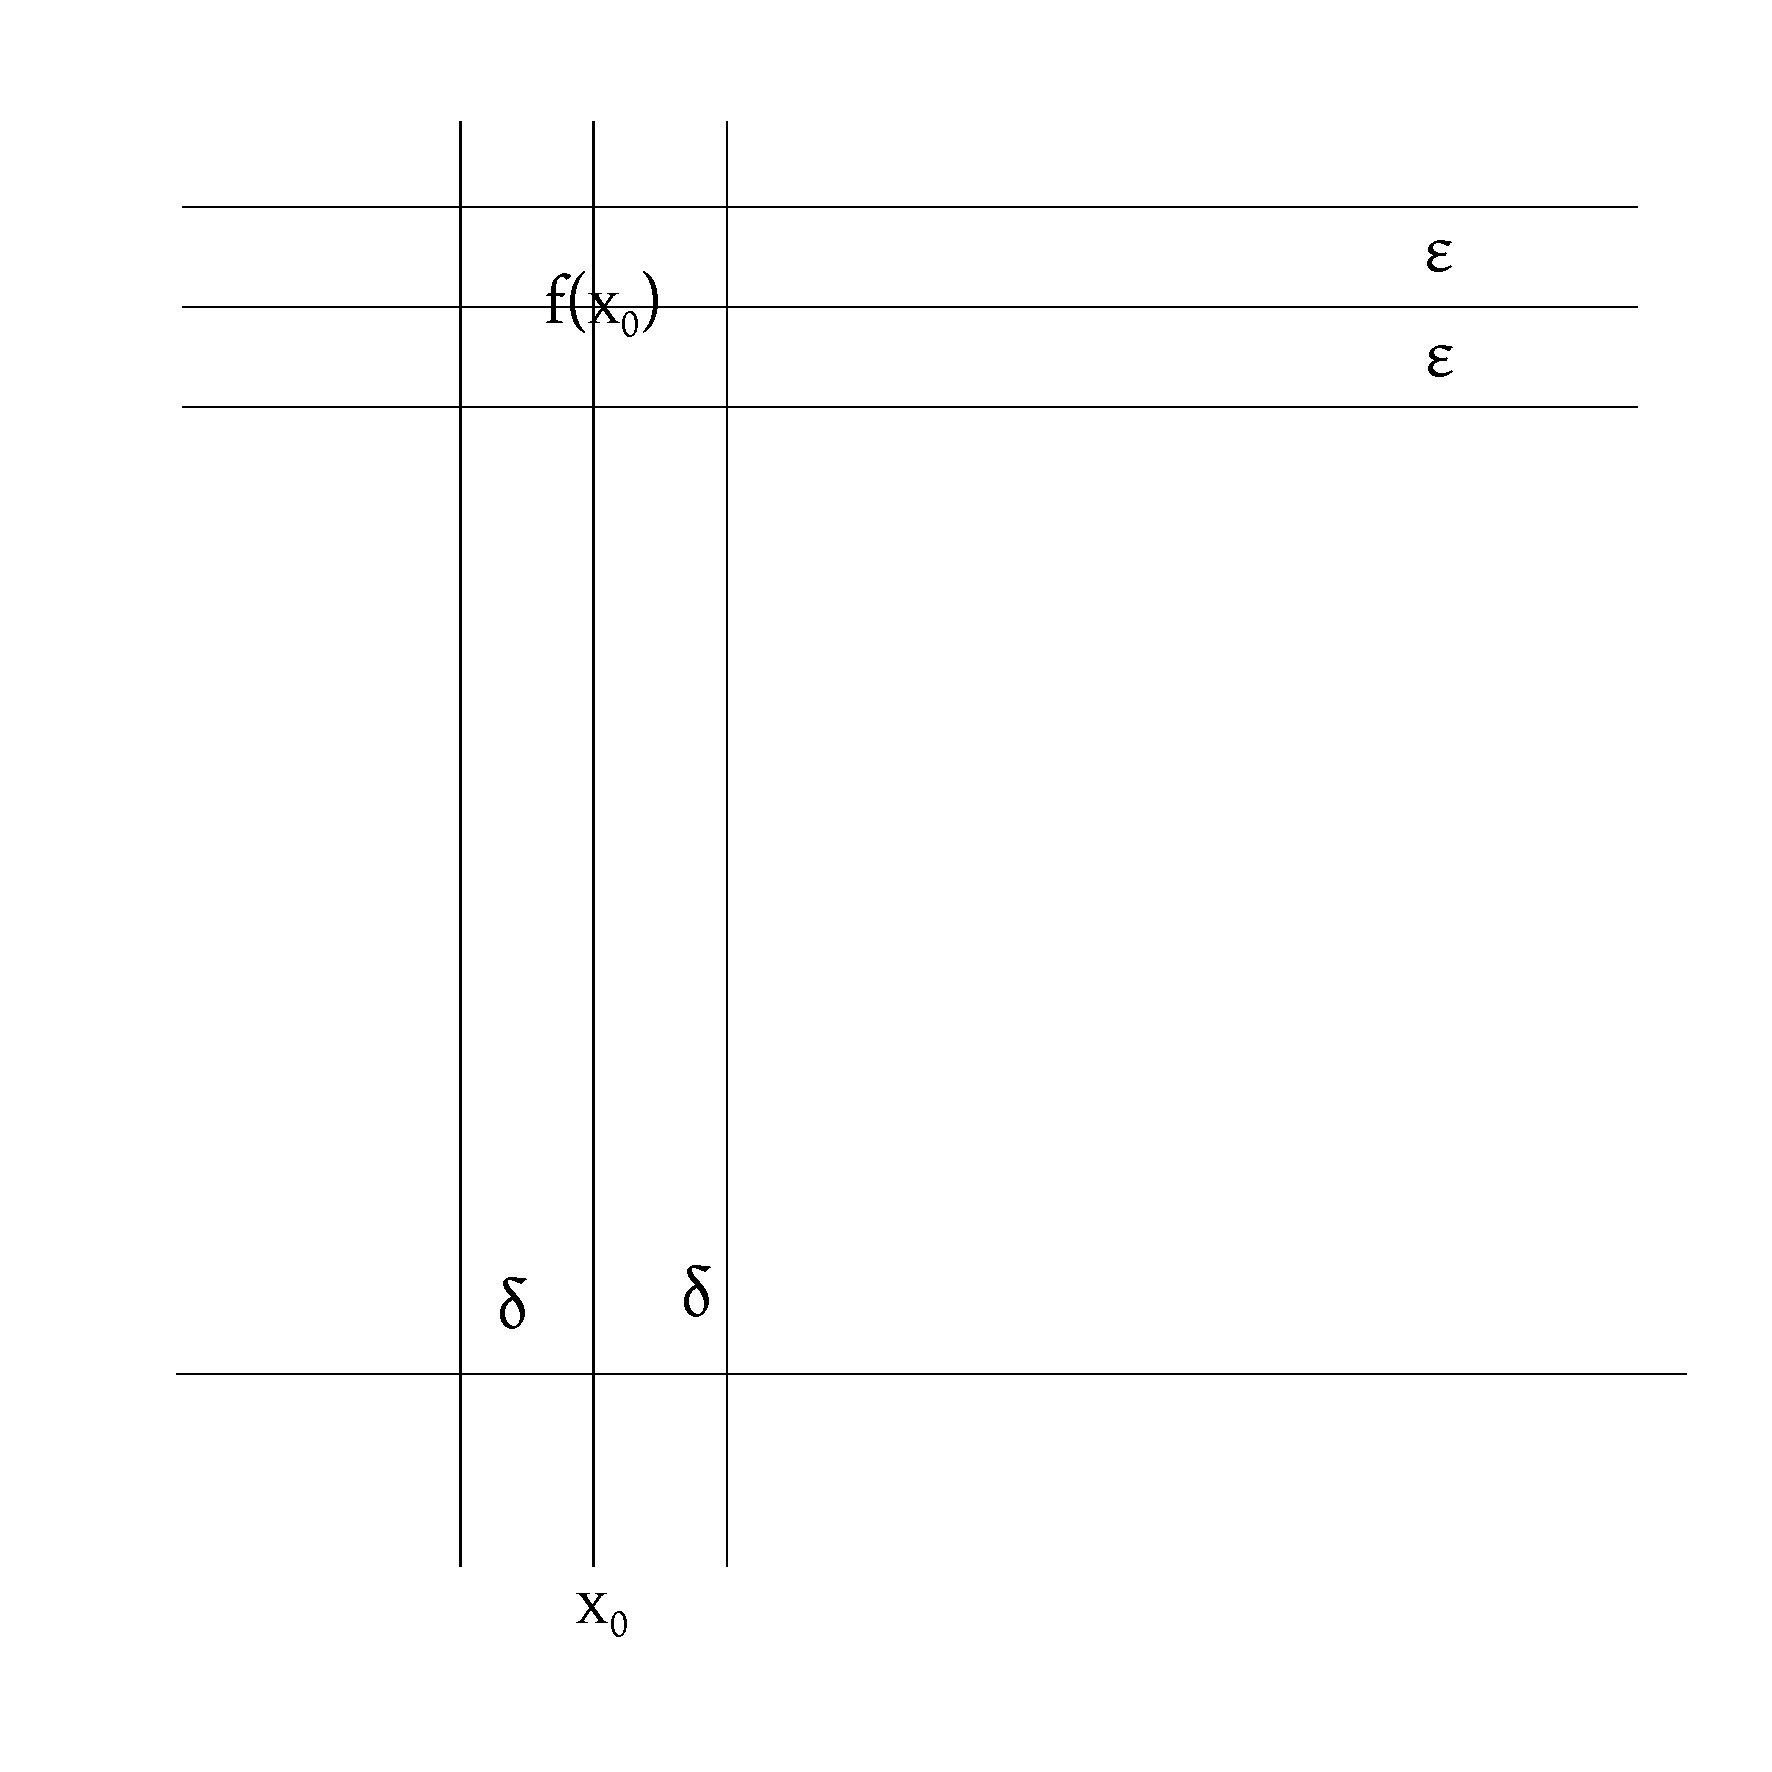
\includegraphics[width=200pt]{img/continuity_revised.pdf}
    \caption{The notion of continuity}
  \end{center}
\end{figure}

$f$ is continuous in $x_0$ if and only if
\[
  \forall \varepsilon > 0 \exists \delta > 0:
  [x \in D \land \abs{x - x_0} < \delta \Rightarrow \abs{f(x) - f(x_0)} < \varepsilon]
\]

Reminder:
Let $z_0 \in U \subseteq \mathbb C$.
$U$ is called environment of $z_0$ if $r > 0$ exists such that $B(z_0, r) \subset U$.

\begin{figure}[!h]
  \begin{center}
    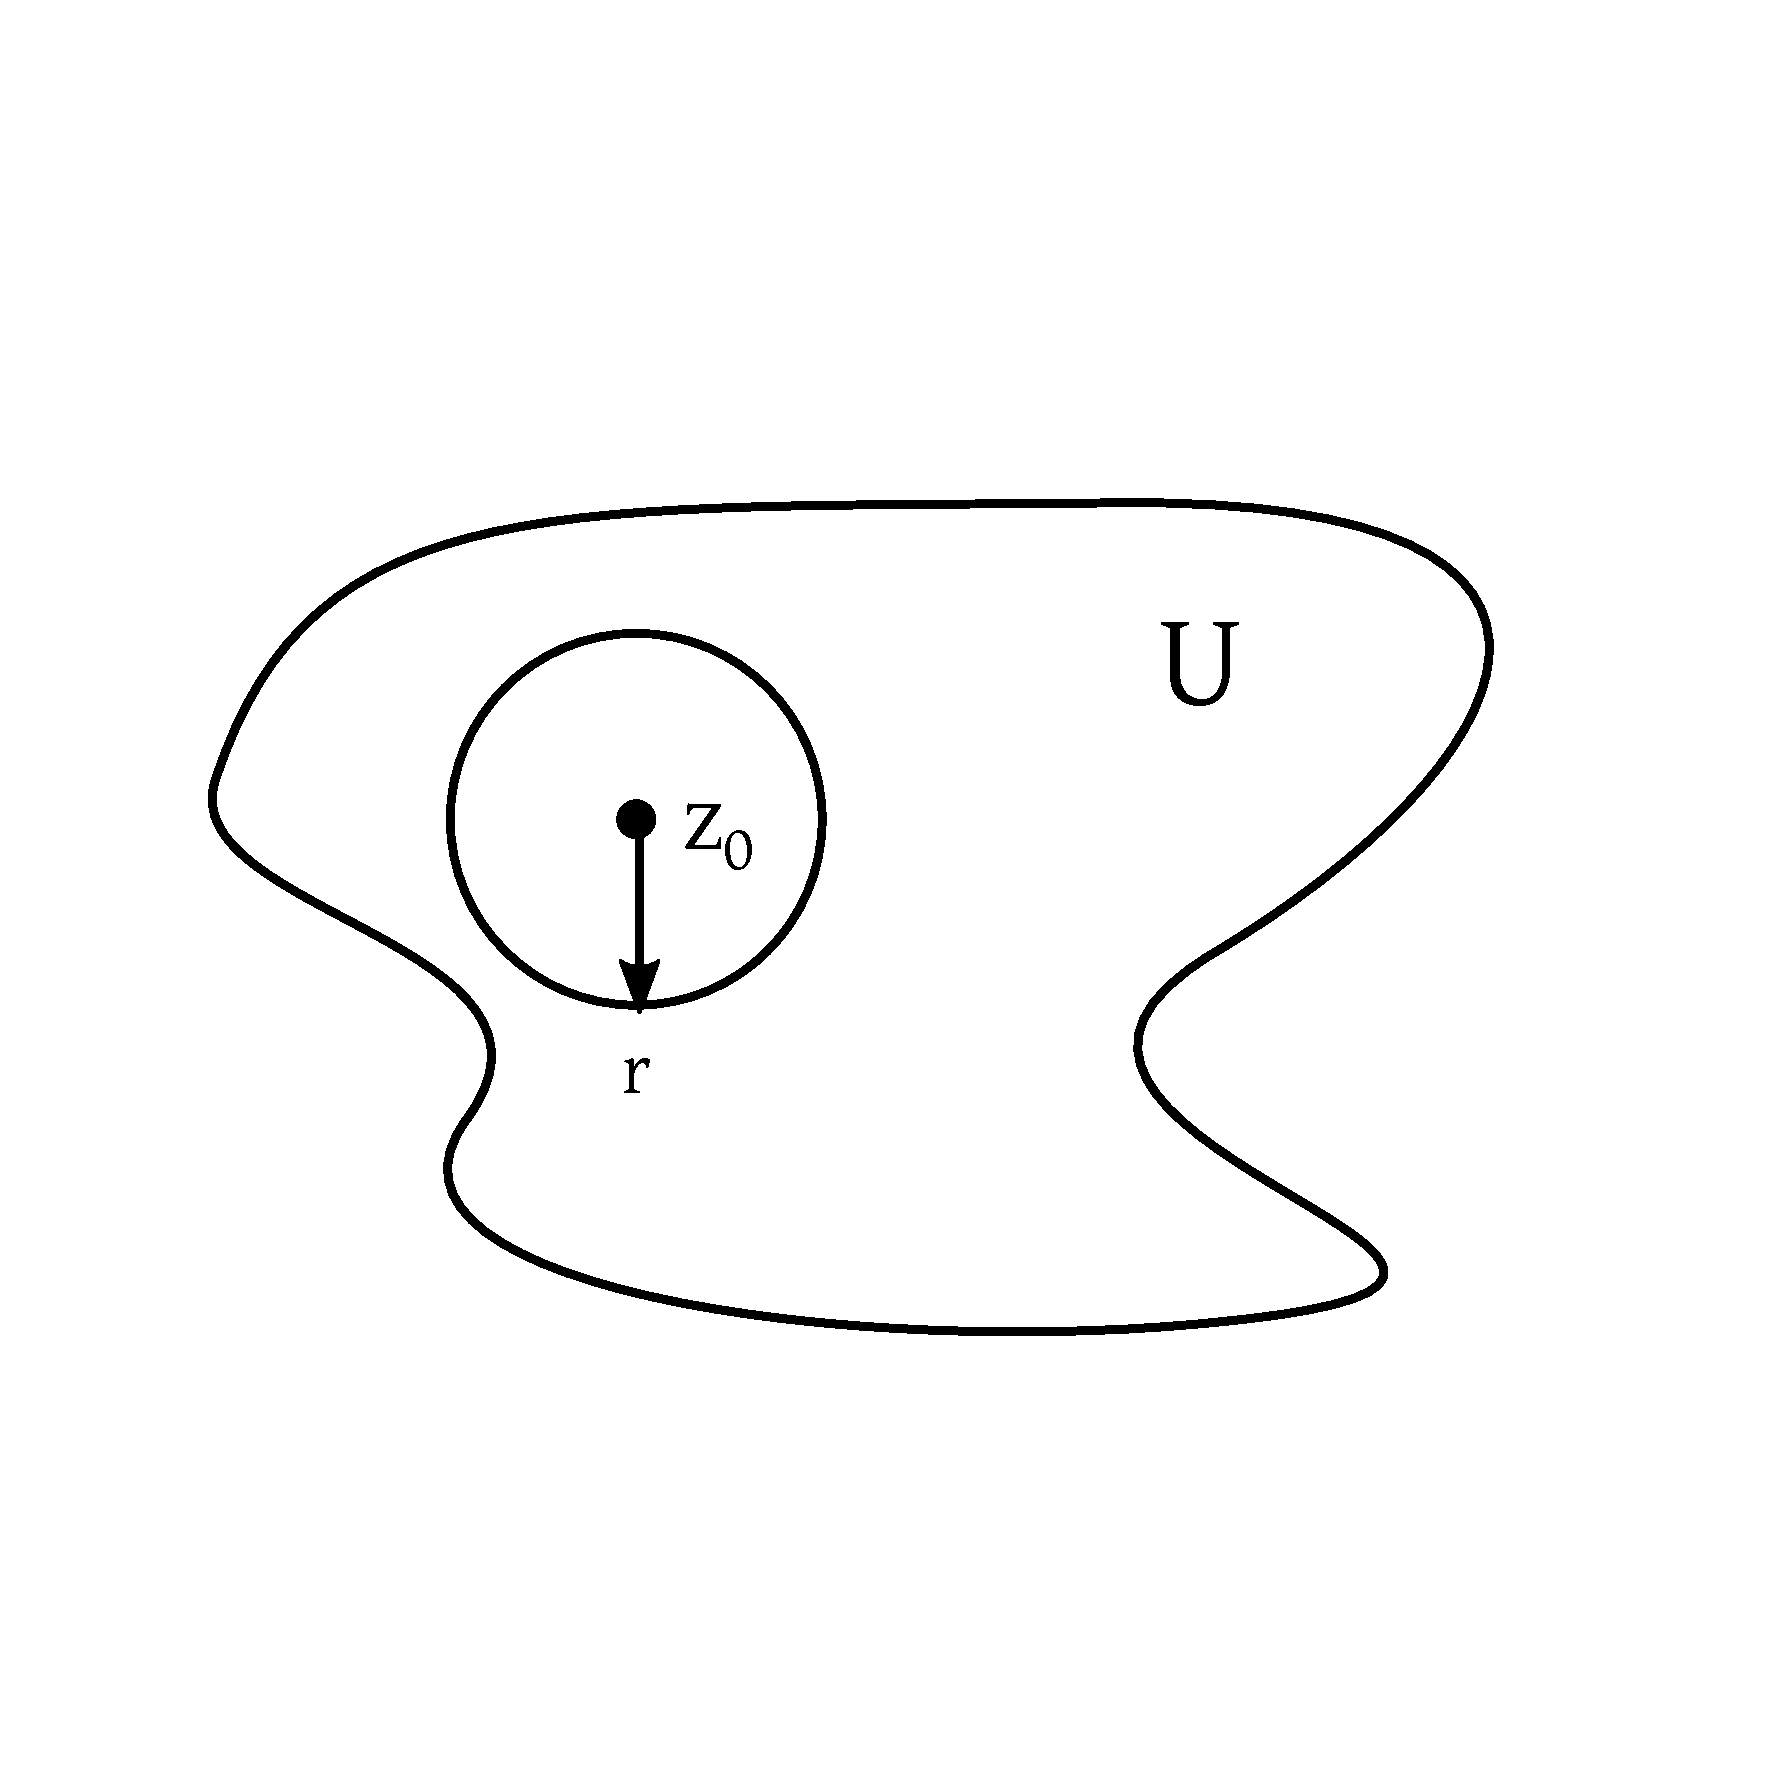
\includegraphics[width=200pt]{img/environment.pdf}
    \caption{Environment with radius $r$}
  \end{center}
\end{figure}

\begin{defi}
  Let $D \subseteq \mathbb C$ and $z_0 \in U \subseteq D$.
  We call $U$ \emph{environment} of $z_0$ \emph{in} $D$ if $\exists r > 0$
  such that $B(z_0, r) \cap D \subseteq U$.
\end{defi}

\begin{figure}[!h]
  \begin{center}
    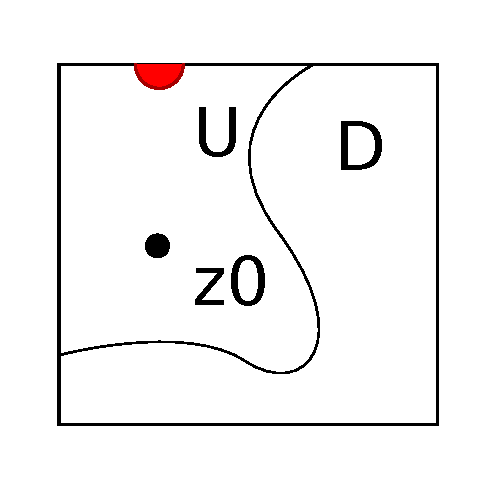
\includegraphics[width=200pt]{img/environment_D_and_U.pdf}
    \caption{Environment $U$}
  \end{center}
\end{figure}

\begin{theorem}
  Let $D \subseteq \mathbb C$ and $f: D \rightarrow \mathbb C$.
  Let $z_0 \in D$. Then $f$ is continuous in $z_0$
  if and only if for every environment $U$ of $y_0 = f(z_0)$
  it holds that $V = f^{-1}(u)$ is an environment of $z_0 \in D$
  (where $f^{-1}$ denotes the preimage).
\end{theorem}

\begin{proof}
  \begin{description}
    \item[$\Rightarrow$] \hfill{} \\
      Let $f$ be continuous in $z_0$ and let $U$ be an environment
      of $y_0 = f(z_0)$, hence $\exists \varepsilon > 0: B(y_0, \varepsilon)
      \subseteq U$ with $y_0 = f(z_0)$. Because $f$ is continuous in $z_0$,
      it holds that
      \[
        \exists \delta > 0:
        \abs{z - z_0} < \delta \land z \in D \Rightarrow
        \underbrace{\abs{f(z) - f(z_0)} < \varepsilon}_{f(z) \in \underbrace{B(f(z_0), \varepsilon)}_{B(y_0, \varepsilon \subseteq U)}}.
      \]

      This requires:
      \[
        \abs{z - z_0} < \delta \land z \in D \Leftrightarrow z \in B(z_0, \delta) \land z \in D
      \]
      \[ \Rightarrow z \in B(z_0, \delta) \cap D \]
      Therefore we can redefine continuity as:
      \[ z \in B(z_0, \delta) \cap D \Rightarrow f(z) \in B(y_0, \varepsilon) \]
      So it holds that
      \[ \forall z \in B(z_0, \delta) \cap D \Rightarrow z \in f^{-1}(B(y_0, \varepsilon)) \subseteq f^{-1}(U) \]
      So it holds that $B(z_0, \delta) \cap D \subseteq f^{-1}(U)$.

    \item[$\Leftarrow$] \hfill{} \\
      Let the preimage of every environment in $y_0$ be an environment of $z_0$ in $D$.
      Let $\varepsilon > 0$ arbitrary. Then it holds that $B(y_0, \varepsilon)$ is an environment of $y_0$.
      By assumption it holds that $V = f^{-1}(B(y_0, \varepsilon))$ is an environment of $z_0$ in $D$,
      hence
      \[ \exists \delta > 0: B(z_0, \delta) \cap D \subseteq f^{-1}(B(y_0, \varepsilon)). \]
      Therefore for $z \in B(z_0, \delta) \cap D$ it holds that $f(z) \in B(y_0, \varepsilon)$.

      In other words:
      \[ \abs{z - z_0} < \delta \land z \in D \Rightarrow |f(z) - \underbrace{f(z_0)}_{= y_0}| < \varepsilon \]
      So $f$ is continuous in $z_0$.
  \end{description}
  This notion of continuity is the most general one accepted by the mathematical community.
  It can be used in all topological spaces.
\end{proof}

\subsection{Variants of continuity}
%
\begin{defi}
  Let $f: D \subseteq \mathbb C \rightarrow \mathbb C$ be a function $f$
  called uniformly continuous in $D$ if
  \[
    \forall \varepsilon > 0 \exists \delta > 0:
    \left[
      \forall z_0, z_1 \in D \text{ with } \abs{z_1 - z_0} < \delta
      \Rightarrow \abs{f(z_1) - f(z_0)} < \varepsilon
    \right]
  \]
  Recognize that $\delta$ only depends on $\varepsilon$,
  meaning that it can be arbitrarily shifted on the $x$-axis ($\delta = \delta(\varepsilon)$).

  Reminder: $f$ is continuous in $D$
  \[
    \Leftrightarrow \forall z_0 \in D \forall \varepsilon > 0 \exists \delta > 0:
    \left[
      \forall z_1 \in D \land \abs{z_1 - z_0} < \delta
      \Rightarrow \abs{f(z_1) - f(z_0)} < \varepsilon
    \right]
  \]
  Recognize that $\delta$ depends on $z_0$ and $\varepsilon$
  ($\delta = \delta(\varepsilon, z_0)$).
  Therefore this second definition provides more freedom to parameter $\delta$.
  So uniform continuity implies continuity in $D$.
\end{defi}
%
\begin{ex}
  Let $f: (0, 1]$ and $f(x) = \frac1x$.
  $f$ is continuous in every point $x_0 \in (0, 1]$.
  However, $f$ is not uniformly continuous.
  \[
    \forall \varepsilon > 0 \exists \delta > 0:
    \left[
      \forall x_0, x_1 \in D \text{ with } \abs{x_0 - x_1} < \delta
      \Rightarrow \abs{\frac1{x_0} - \frac1{x_1}} < \varepsilon
    \right]
  \]
  The negation is given with:
  \[
    \exists \varepsilon > 0 \forall \delta > 0:
    \left[
      \exists x_0, x_1 \in D \text{ with }
      \abs{x_0 - x_1} < \delta \land \abs{\frac1{x_0} - \frac1{x_1}} \geq \varepsilon
    \right]
  \]
  We look at $\varepsilon = 1$.
  Let $\delta > 0$ arbitrary. We choose $x_0 = \frac1n$ and $x_1 = \frac1{n+1}$
  for appropriate $n \in \mathbb N_+$. Then it holds that
  \[
    \abs{x_0 - x_1} = \abs{\frac1n - \frac1{n+1}} =
    \frac{n + 1 - n}{n (n + 1)} = \frac1{n (n + 1)}
    \underbrace{<}_{\text{for } n \in \mathbb N_+}
    \frac1n
    <
    \delta
  \]
  if $n > \frac1\delta$
  \[
    \abs{\frac1{x_0} - \frac1{x_1}}
    = \abs{\frac1{\frac1n} - \frac1{\frac1{n+1}}}
    = \abs{n - (n + 1)}
    = \abs{-1}
    = 1
  \]
  Therefore $f(x) = \frac1x$ is not uniformly continuous in $(0, 1]$.

  Remark: $f(x) = \frac1x$ is uniformly continuous in $D = [\frac1{100}, 1]$,
  but not in $\mathbb R$.
\end{ex}
%
\index[English]{Lipschitz continuity}
\index[German]{\foreignlanguage{ngerman}{Lipschitz Stetigkeit}}
\begin{defi}[Lipschitz continuity]
  Another notion of continuity is given by \fbox{Rudolf Lipschitz (1832--1903)}.

  $f: D \subset \mathbb C \rightarrow \mathbb C$ is called Lipschitz continuous
  if $k \geq 0$ exists such that
  \[
    \forall z_1, z_2 \in D:
    f(z_1) - f(z_2) \leq k \abs{z_1 - z_2}
  \]
  The value $k$ is called Lipschitz constant for $f$.
\end{defi}
%
\index[English]{Hölder continuity}
\index[German]{\foreignlanguage{ngerman}{Hölder Stetigkeit}}
\begin{defi}[Hölder continuity]
  Yet another notion of continuity is given by \fbox{Otto Hölder (1859--1937)}.

  $f$ is called Hölder continuous with exponent $H \in (0, 1]$ if there exists
  $k > 0$ such that
  \[ \forall z_1, z_2 \in D: \abs{f(z_1) - f(z_2)} \leq k \abs{z_1 - z_2}^H \]
\end{defi}
%
\begin{cor}
  A hierarchy for those continuity notion is given:

  Lipschitz continuous $\subseteq$ uniformly continuous $\subseteq$ continuous in $D$.
\end{cor}
%
\begin{theorem}
  Let $K \subseteq \mathbb C$ be compact. Let $f: K \rightarrow \mathbb C$ be continuous
  in $K$. Then $f(K) = \set{y = f(z): z \in K} \subset \mathbb C$ is compact in $\mathbb C$.
\end{theorem}
\begin{proof}
  Every sequence $(y_n)_{n \in \mathbb N}$,
  with $y_n = f(z_n)$ and $z_n \in K$ where $y_n \in f(K)$,
  has a convergent subsequence. The sequence of preimage values $(z_n)_{n \in \mathbb N}$
  is a sequence in $K$ which, followingly, has a convergent subsequence.
  Let $(z_{n_k})_{k \in \mathbb N}$
  $\lim_{k \to \infty} z_{n_k} = z \in K$.
  Because of the sequence criterion for continuity if holds that
  \[ \lim_{k \to \infty} y_{n_k} = \lim_{k \to \infty} f(z_{n_k}) = f(z) \in f(k) \]
  with $y = f(k)$.
  So $(y_n)_{n \in \mathbb N}$ has a convergent subsequence with limes $y \in f(K)$.
  Therefore $f(K)$ is compact.
\end{proof}
%
\index[English]{global maximum}
\index[German]{\foreignlanguage{ngerman}{Globales Maximum}}
\begin{defi}
  Let $f: D \rightarrow \mathbb R$ and $D \subseteq \mathbb C$. A point $z_{\text{max}} \in D$
  is called global maximum of $f$ if $f(z_{\text{max}}) \geq f(z) \quad\forall z \in D$.
\end{defi}

\begin{figure}[!h]
  \begin{center}
    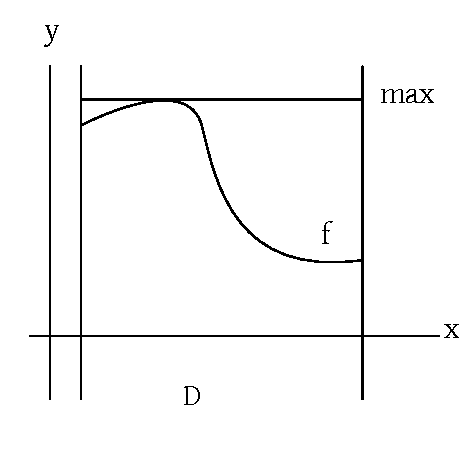
\includegraphics[width=200pt]{img/global_maximum.pdf}
    \caption{Illustration of a global maximum}
  \end{center}
\end{figure}

\begin{defi}
  Let $f: K \rightarrow \mathbb R$ ($K \subseteq \mathbb C$) is continuous in $K$
  and $K$ is compact in $\mathbb C$. Then $f$ has a global maximum and a global
  minimum.
\end{defi}

\begin{rem}
  For non-compact definition sets this statement is not generally true.
  For example, $f(x) = \frac1x$ in $D = (0, 1)$ has neither a global maximum
  nor a global minimum.
\end{rem}
\begin{proof}
  \[ f(K) \subseteq \mathbb R \]
  is compact (because of the previous theorem) and therefore bounded and
  closed in $\mathbb R$ (by Theorem by Bolzano-Weierstrass).
  Because $f(K)$ is bounded, $f(K)$ has a supremum $\zeta^*$ and an infimum $\zeta_*$
  (supremum property). Supremum and infimum are contact points of $f(K)$.
  Because $f(K)$ is closed it holds that
  \[ \zeta^* \in f(K) \text{ and } \zeta_* \in f(K) \]
  Therefore there exists $z_{\text{min}} \in K$ with $f(z_{\text{min}}) = \zeta_*$
  and $z_{\text{max}} \in K$ with $f(z_{\text{max}}) = \zeta^*$.
  Because $f(K)$ is closed, it holds that $\zeta^* \in f(K)$ and $\zeta_* \in f(K)$.
  Therefore there exists $z_{\text{min}} \in K$ with $f(z_{\text{min}}) = \zeta_*$.
  and $f(z_{\text{max}}) \in K$ with $f(z_{\text{max}}) \geq y$, therefore
  $\forall z \in K: f(z_{\text{max}}) \geq f(z)$.

  Therefore $z_{\text{max}}$ is a global maximum. The analogous statement holds
  for $\zeta_*$ and a global minimum.
\end{proof}

\begin{theorem}[A very universal theorem about maxima]
  A continuous function has a global maximum in a compact domain.
\end{theorem}

Using this method to show existence of a value is called
\enquote{direct method of variation computations}.

\meta{lecture}{8th of January 2016}{Wolfgang Ring}
%
Continuity and compactness implies existence of a maximum and minimum.

\enquote{Direct method of calculus of variations} (dt. \foreignlanguage{ngerman}{\enquote{direkte Methode der Variationsrechnung}}).

\begin{theorem}[Intermediate value theorem for continuous functions]
  Let $f: [a, b] \to \mathbb R$ be continuous with $a \leq b$. Let
  \begin{align*}
    m^* &= \max\set{f(x): x \in [a, b]} \\
    m_* &= \min\set{f(x): x \in [a, b]}
  \end{align*}
  $m^*$ and $m_*$ exist because $[a, b]$ is compact (bounded and closed).

  Let $m_* \leq \eta \leq m^*$.

  Then there exists $\xi \in [a, b]$ with $f(\xi) = \eta$.
  The function $f$ takes any value for some $x$ in $m_*$ and $m^*$.
  Compare with Figure~\ref{img:zeta-in-ab}.

  \begin{figure}[!h]
    \begin{center}
      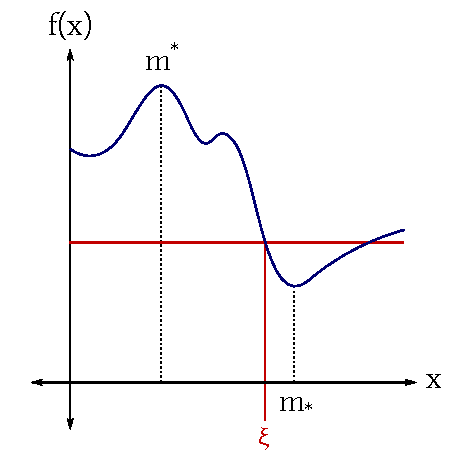
\includegraphics{img/zeta_in_ab_interval.pdf}
      \caption{$\zeta$ in $[a, b]$}
      \label{img:zeta-in-ab}
    \end{center}
  \end{figure}
\end{theorem}
\begin{proof}
  Let $a_0 \in [a, b]$ such that $f(a_0) = m_*$ and $b_0 \in [a, b]$ such that $f(b_0) = m^*$.
  Without loss of generality: $a_0 = b_0$.
  If $a_0 > b_0$ it holds that $\max\set{f(x): x \in [a,b]} = f(b_0) = f(a_0) = \min\set{f(x): x \in [a, b]}$.
  If $\max = \min$, then $f$ is constant, hence $f(x) = m_* = m^* \quad\forall x \in [a, b]$.
  \[ m_* = \eta \leq m^* \Rightarrow \eta = m_* = m^* \land f(x) = \eta \quad\forall x \in [a,b] \]
  Consider $a_0 \leq b_0$. We know, $f(a_0) = m_* \leq \eta \leq m^* = f(b_0)$.
  We use nested intervals:

  Assume $I_n = [a_n, b_n]$ for $n \in \mathbb N$ was already found with the property $f(a_n) \leq \eta \leq f(b_n)$.
  Let $m_n = \frac12 (a_n + b_n)$ be the midpoint of $I_n$.
  \begin{description}
    \item[Case $f(m_n) \geq \eta$]
      If $f(m_n) \geq \eta$ we set $b_{n+1} > m_n \land a_{n+1} > a_n$ (compare Figure~\ref{img:am_bm})
      \begin{figure}[!h]
        \begin{center}
          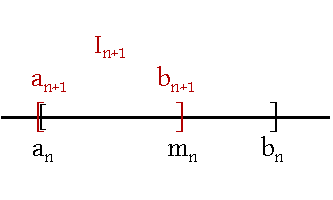
\includegraphics{img/am_bm.pdf}
          \caption{Interval $I_{n+1}$}
        \end{center}
      \end{figure}
      and it holds that $f(a_{n+1}) = f(a_n) \leq \eta$ and $f(b_{n+1}) = f(m_n) \geq \eta$.
      Furthermore $\abs{I_{n+1}} = \frac12 \abs{I_n}$.
    \item[Case $f(m_n) < \eta$]
      Let $a_{n+1} = m_n$ and $b_{n + 1} = b_n$.
      \[ I_{n+1} = [a_{n+1}, b_{n+1}] \]
      \[ f(a_{n+1}) = f(m_n) < \eta \]
      \[ f(b_{n+1}) = f(b_n) \geq \eta \]
      \[ \abs{I_{n+1}} = \frac12 \abs{I_n} \]
  \end{description}
  Nested interval $\seq{I_n}$ has the property:
  \[ I_{n+1} \leq I_n \qquad \abs{I_n} = \left(\frac12\right)^n \cdot \abs{I_0} = \left(\frac12\right)^n \cdot (b_0 - a_0) \]
  and $f(a_n) \leq \eta \leq f(b_n)$. $\seq{I_n}$ is are nested intervals.
  Let $\xi \in \bigcap_{n\in\mathbb N} I_n$ and it holds that $\abs{\xi - a_n} \leq \abs{b_n - a_n} = \underbrace{\left(\frac12\right)^n \cdot (b_0 - a_0)}_{\to 0 \text{ for } n \to \infty}$.
  Therefore $\lim_{n\to\infty} a_n = \xi$ and
  \[
    \abs{b_n - \xi} \leq \abs{b_n - a_n}
    = \underbrace{\left(\frac12\right)^n (b_0 - a_0)}_{\to 0 \text{ for } n \to \infty}.
  \]
  So $\lim_{n\to\infty} b_n = \xi$.

  Because $f$ is continuous on $[a, b]$, it holds that
  \[ \eta \leq f(b_n) \quad\forall n \in \mathbb N \Rightarrow \eta \leq \lim_{n\to\infty} f(b_n) \]
  \[ \text{continuity } \Rightarrow \lim_{n\to\infty} f(b_n) = f(\xi) \]
  So,
  \[ \eta \leq \lim_{n\to\infty} f(b_n) = f(\xi) = \lim_{n\to\infty} f(a_n) \leq \eta. \]
  Therefore $\eta = f(\xi)$.
\end{proof}
\index[English]{Bisection method}
\index[German]{Bisektionsverfahren}
\begin{rem}
  From this we can derive continuity for a numerical algorithm for solving $f(x) = \eta$.
  It's called \emph{bisection method}.
\end{rem}
\begin{rem}
  Often the intermediate value theorem is defined as:

  Let $\eta$ be between $f(a)$ and $f(b)$. Then there exists $\xi \in [a, b]$
  such that $f(\xi) > \eta$. Obviously because $m_* \leq f(a)$ and $f(b) \leq m^*$.
\end{rem}
\begin{defi}[Limes of a function]
  Let $D \subseteq \mathbb C$ and $f: D \to \mathbb C$. Let $z$ be a limit point of $D$.
  We say, that $f$ in $z$ has the limes $w$ if the function
  \[
    \hat{f}: D \cup \set{z} \to \mathbb C
  \] \[
    \hat{f}(\xi) = \begin{cases}
      f(\xi) & \text{if } \xi \neq z \\
      w & \text{if } \xi = z
    \end{cases}
  \]
  is continuous. We denote $\lim_{\xi \to z} f(\xi)$.
\end{defi}
\begin{ex}
  See Figures~\ref{img:cont-ex1}, \ref{img:cont-ex2} and \ref{img:cont-ex3}.
  \begin{figure}[p]
    \begin{center}
      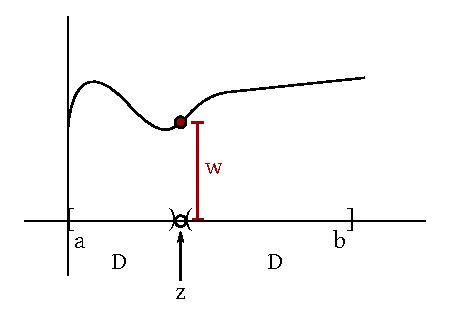
\includegraphics{img/continuity_example_1.pdf}
      \caption{Example 1 with $D = [a, b] \setminus \set{z}$ and $w = \lim_{\xi \to z} f(\xi)$}
      \label{img:cont-ex1}
    \end{center}
    \begin{center}
      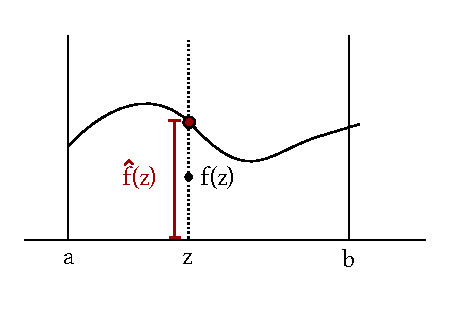
\includegraphics{img/continuity_example_2.pdf}
      \caption{
        Example 2 which defines function new in point $z$ with $D = [a,b]$ and $\lim_{\xi \to z} f(\xi)$.
        $f$ is not continuous in $z$, but $\hat{f}$ is continuous in $z$.
      }
      \label{img:cont-ex2}
    \end{center}
  \end{figure}
  \begin{figure}[p]
    \begin{center}
      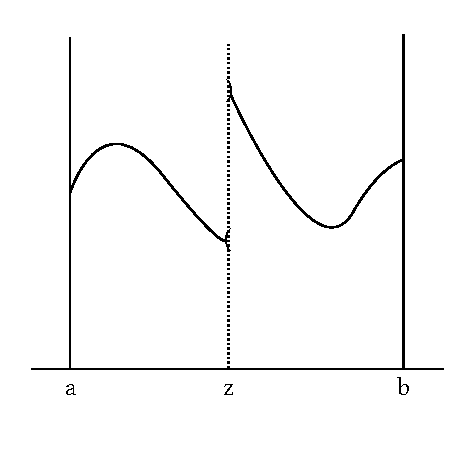
\includegraphics{img/continuity_example_3.pdf}
      \caption{
        Example 3 with $D = [a, b] \setminus \set{z}$.
        $f$ does not have a limes in $z$. Due to the jumping point, it is not a continuous function.
        Therefore we cannot find $\varepsilon$.
        We say $\hat{f}$ is a continuous continuation of $f$ in point $z$.
      }
      \label{img:cont-ex3}
    \end{center}
  \end{figure}
\end{ex}
\begin{lemma}
  Let $f: D \to \mathbb C$ given and $z$ is a limit point of $D \subseteq \mathbb C$.
  Then $f$ has a limes $w \in \mathbb C$ if and only if one of the equivalent conditions hold.
  \begin{itemize}
    \item
      $\forall \varepsilon > 0 \exists \delta > 0 \forall \xi \in D:
      \abs{z - \xi} < \delta
      \Rightarrow |\underbrace{f(\xi)}_{\hat{f}(\xi)} - \underbrace{w}_{\hat{f}(z)}| < \varepsilon$
      \begin{center}
        \enquote{Continuity of $\hat{f}$}
      \end{center}
    \item
      $\forall \seq{\xi}$ with $\xi_n \in D \setminus \set{z}$ and $\lim_{n\to\infty} \xi_n = z$ holds.
      \[ \lim_{n\to\infty} f(\xi_n) = w \]
      \begin{center}
        \enquote{Sequence criterion for $\hat{f}$}
      \end{center}
  \end{itemize}
\end{lemma}
\begin{ex}
  $f: \mathbb C \setminus \set{1} \to \mathbb C$ with
  \[ f(z) = \frac{z^2 - 1}{z - 1} \]
  For $z \neq 1$ it holds that:
  \[ f(z) = \frac{(z - 1)(z + 1)}{(z - 1)} = (z + 1) \]
  Let
  \[
    \hat{f}(z) = \begin{cases}
      f(z) & \text{if } z \neq 1 \\
      2 & \text{if } z = 1
    \end{cases}
  \]
  $\hat{f}(z) = z + 1$ in $\mathbb C$ is continuous.
  $f$ has limes $w = 2$ in point $z > 1$.
\end{ex}
\begin{ex}
  Let $s \in \mathbb Q \setminus \set{0}$ and $D = (-1, \infty) \setminus \set{0}$
  \[ f(x) = \frac{(1 + x)^s - 1}{x} \]
  It holds that $\lim_{x \to 0} f(x) = s$.
  \begin{proof}[for $\abs{x} < 1$]
    \[ (1 + x)^s = \sum_{k = 0}^\infty \binom sk x^k \Rightarrow \frac{(1 + x)^s - 1}{x} \]
    \[
      \Rightarrow \frac{(1 + x)^s - 1}{x}
      = \frac{\sum_{k=1}^\infty \binom sk x^k}{x}
      = \sum_{k=1}^\infty \binom sk \cdot x^{k-1}
    \] \[
      \lim_{x \to 0} \underbrace{\left(
        \sum_{k=1}^\infty \binom sk x^{k-1}
      \right)}_{f(x)}
      = \sum_{k=1}^\infty \binom sk 0^{k-1}
      = \binom s1 = s
    \]
    We need the following theorem: A power series is in its convergence
    radius a continuous function.
  \end{proof}
\end{ex}

\section{Differential calculus}
%
Let $f: (a, b) \to \mathbb R$ be given. with $a < b$.

Idea: We want $f$ close to point $x_0 \in (a, b)$
be approximated by a linear-affine function $a(x) = k(x - x_0) + d$.
%
\[ a(x) = k (x - x_0) + d = kx + \underbrace{(-kx_0 + d)}_{\tilde d} = kx + \tilde d \]
$\tilde a(x) = kx$ is linear. Linear and constant functions are linear affine.
$a$ should (at least) cross point $x_0$, ie. $f(x_0)$. Compare with Figure~\ref{img:differential}.

\begin{figure}[!t]
  \begin{center}
    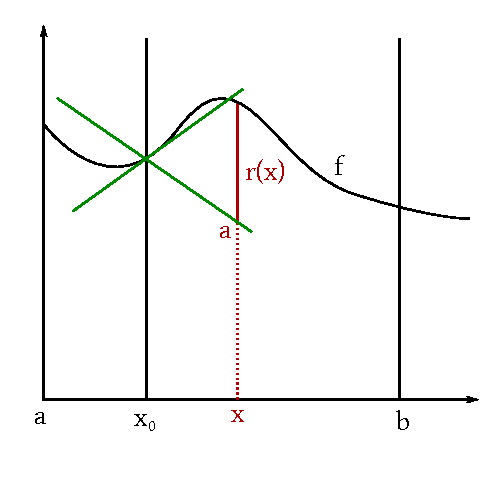
\includegraphics{img/differential.pdf}
    \caption{Differential $f$ in $x_0$}
    \label{img:differential}
  \end{center}
\end{figure}

\[ \Rightarrow a(x_0) = k (\underbrace{x_0 - x_0}_{0}) + a \overset!= f(x_0) \Rightarrow d = f(x_0) \]
\[ \Rightarrow a(x) = k (x - x_0) + f(x_0) \]

How should we select $k$ such that the approximation of $f$ is best possible by selection of $a$.
We consider the deviation.

\[ f(x) = f(x) - a(x) \]

$r(x)$ should be as small as possible in $x_0$.
Therefore $\lim_{x \to x_0} r(x) = 0$.

\[ \lim_{x \to x_0} r(x) = \lim_{x \to x_0} [f(x) - f(x_0) - k \cdot (x - x_0)] = 0 \quad\forall k \]

We need: $r(x)$ should converge to $0$ very quickly for $x \to x_0$.

Idea: Require that $\lim_{x \to x_0} \frac{r(x)}{x - x_0} = 0$.
$\frac1{x - x_0}$ is unbounded close to $x_0$. $\lim_{x \to x_0} \frac{r(x)}{x - x_0} = 0$ means
$\lim_{x \to x_0} \abs{\frac{r(x)}{x - x_0} - 0} = 0$

\[
  \Rightarrow \lim_{x \to x_0}
  \abs{\frac{f(x) - f(x_0) - k \cdot (x - x_0)}{x - x_0}}
  = \lim_{x \to x_0} \abs{\frac{f(x) - f(x_0)}{x - x_0} - k}
\]
Hence,
\[
  \Rightarrow k = \lim_{x \to x_0} \frac{f(x) - f(x_0)}{x - x_0}
\]
with
\[ \lim_{x \to x_0} \frac{r(x)}{x - x_0} = 0, \]
$k$ is uniquely identified with
\[ \lim_{x \to x_0} \frac{f(x) - f(x_0)}{x - x_0} \]

\meta{lecture}{13th of January 2016}{Wolfgang Ring}

\begin{figure}[!h]
  \begin{center}
    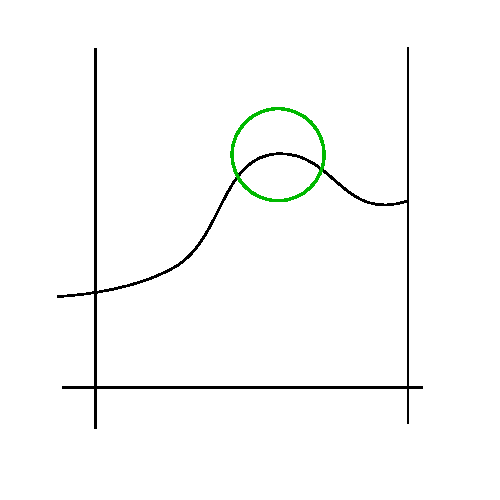
\includegraphics{img/radius.pdf}
    \caption{Derivative}
    \label{img:deriv-radius}
  \end{center}
\end{figure}

TODO: another figure missing

\[ y = kx + d \]
\[ d = k \cdot(x_0) - k \cdot x_0 \]

TODO: missing a few lines

\index[English]{Landau symbols}
\index[German]{\foreignlanguage{ngerman}{Landau Symbole}}
\begin{defi}[Landau's symbols]
  Let $g: D \to \mathbb C$, $D \subseteq \mathbb C$.
  Let $z_0$ be a limit point of $g$ and assume $g$ has a limit point $0$ for $z \to z_0$.
  Therefore,
  \[ \forall \varepsilon > 0 \exists \delta > 0: \forall z \in D \land \abs{z - z_0} < \delta \]
  where $z \neq z_0$.
  \[ \Rightarrow \abs{g(z) - 0} < \varepsilon \]
  We say that $y$ is \emph{of order $\mathcal{O}(n)$} in point $z_0$,
  if $k \geq 0$ and some $r > 0$ such that
  \[ \abs{g(z)} \leq K \abs{z - z_n}^n \quad\forall z \in D \text{ with } \abs{z - z_0} < r \land z \neq z_0 \]
  We denote it with $g(z) = \mathcal O(\abs{z - z_0}^n)$.

  We say that $g$ is of order $o(n)$ if $r > 0$ and some function $k: (0, r) \to \mathbb R^+$
  with $\lim_{x\to 0} k(x) = 0$ exists, such that
  \[
    \abs{g(z)} \leq k(\abs{z - z_0}) \cdot \abs{z - z_0}^n
    \forall z \in D \text{ with } \abs{z - z_0} < r \land z \neq z_0
  \]
  We denote,
  \[ g(z) = o(\abs{z - z_0}^n) \]
\end{defi}
\begin{cor}
  It holds that,
  $g: \mathcal O(\abs{z - z_0}^n) \Leftrightarrow \exists r > 0$ such that
  \[ \frac{\abs{g(z)}}{\abs{z - z_0}^n} \]
  is bounded in $B(z_0, z) \setminus \set{z_0}$ and $g = o(\abs{z - z_0}^n)$,
  if $\exists r > 0$ such that $\frac{\abs{g(z)}}{\abs{z - z_0}^n}$ in point
  $z_0$ has limit point $0$.
\end{cor}
\index[English]{Slope}
\index[German]{\foreignlanguage{ngerman}{Steigung}}
\begin{cor}
  For determination of the slope $k$ for the best-achievable linear-affine approximation
  of $f$ it must hold that
  \[ f(x) - (f(x_0) - k (x - x_0)) = o(\abs{x - x_0}) \]
\end{cor}
\index[English]{Derivative of a function $f$}
\index[German]{\foreignlanguage{ngerman}{Ableitung einer Funktion $f$}}
\index[English]{differentiable}
\index[German]{\foreignlanguage{ngerman}{Ableitbarkeit}}
\begin{defi}
  Let $f: (a, b) \to \mathbb R$ and $x_0 \in (a, b)$. We claim that $f$ in $x_0$
  is \emph{differentiable}, if the limit point of the function $\frac{f(x) - f(x_0)}{x - x_0}$
  exists. The corresponding limit point $k = \lim_{x\to x_0} \frac{f(x) - f(x_0)}{x - x_0}$
  is called \emph{derivative of $f$ in $x_0$}.

  We can compute $k$ using $k = f'(x_0)$.

  Alternatively: $f$ is differentiable in $x_0$ if $x \in \mathbb R$ exists,
  such that
  $r: (a, b) \setminus \set{0} \to \mathbb R$
  with
  $r(x)  = f(x) - f(x_0) - k(x - x_0)$
  is of order $o(1)$ in $x_0$.
  \[ f(x) - f(x_0) - k(x - x_0) = \mathcal O(\abs{x - x_0}) \]

  The second definition is more general and can also be applied for functions
  $f: \mathcal O \subseteq \mathbb R^n \to \mathbb R^n$.
\end{defi}
%
\begin{cor}
  Let $f: (a, b) \to \mathbb R$ be differentiable in $x_0 \in (a, b)$. Then
  the function
  \[
    \varphi(x) = \begin{cases}
      \frac{f(x) - f(x_0)}{x - x_0} & \text{if } x \in (a, b) \setminus \set{x_0} \\
      f'(x_0) & \text{if } x = x_0
    \end{cases}
  \]
  $\varphi: (a,b) \to \mathbb R$ and $\varphi$ is continuous in $x_0$.

  Show that $\lim_{x\to x_0} \varphi(x) = \varphi(x_0)$.

  \[ f(x) = f(x_0) + \varphi(x)(x - x_0) \]
  because $\varphi(x) = \frac{f(x) - f(x_0)}{x - x_0}$ for $x \neq x_0$.
  $f(x)$ is constant, $\varphi(x)$ is continuous in $x_0$ and $(x - x_0)$ is continuous in $(a, b)$.
  For $x = x_0$, $f(x) = f(x_0) + \varphi(x)(x - x_0)$ holds as well.

  Therefore all expressions of $f(x_0) + \varphi(x)(x - x_0)$ are continuous in $x_0$,
  followingly $f$ is continuous in $x_0$.
\end{cor}
\index[English]{tangent}
\index[German]{\foreignlanguage{ngerman}{Tangente}}
\begin{lemma}
  Let $f: (a, b) \to \mathbb R$ be differentiable in $x_0 \in (a, b)$.
  \[ k = \lim_{x \to x_0} \frac{f(x) - f(x_0)}{x - x_0} \]
  is slope of affine function, which approximates $f$ in $x_0$.

  Plot of this function:
  \[ y(x) = f'(x_0) (x - x_0) - f(x_0) \]
  is called \emph{tangent} of $f$ in $x_0$.

  \begin{figure}[t]
    \begin{center}
      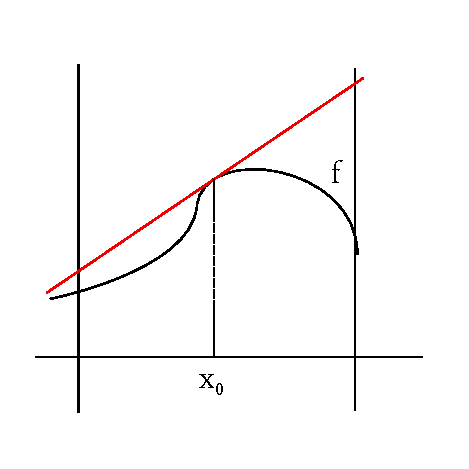
\includegraphics{img/tangent.pdf}
      \caption{Tangent of $f$ in $x_0$}
    \end{center}
  \end{figure}
\end{lemma}

\meta{lecture}{14th of Jan 2016}{Wolfgang Ring}
%
\begin{theorem}[Convergence, limes and differentiable functions]
  Let $f: (a, b) \to \mathbb R$ be differentiable in $x_0 \in (a, b)$.
  Therefore the equivalent defining properties hold.
  \begin{enumerate}
    \item $\forall \varepsilon > 0 \exists \delta > 0 \forall x \in (a, b)$
      with $\abs{x - x_0} < \delta$ and $x \neq x_0$ it holds that
      $\abs{\frac{f(x) - f(x_0)}{x - x_0} - f'(x_0)} < \varepsilon$.
      This constitutes a definition of the limes.
    \item For all $\seq{\xi_n}$ with $\xi_n \in (a, b)$ and $\xi_n \neq x_0$
      and $\lim_{n\to\infty} \xi_n = x_0$, it holds that
      \[
        \left(\frac{f(\xi_n) - f(x_0)}{\xi_n - x_0}\right)_{n\in\mathbb N}
        \text{ is convergent towards } f'(x_0)
      \]
      This is the sequence criterion for the limes.
    \item For all $\varepsilon > 0$, there exists some $\delta > 0$ such
      that $\forall x \in (a, b)$ with $\abs{x - x_0} < \delta$ it holds that
      \[ \abs{f(x) - f(x_0) - f'(x_0)(x - x_0)} \leq \varepsilon \abs{x - x_0} \]
      holds also for $x = x_0$.
  \end{enumerate}
  The (3) implies the (1): Assume (3) holds and
  choose $\delta$ such that $\forall \abs{x - x_0} < \delta$ it holds that
  \[
    \abs{f(x) - f(x_0) - f'(x_0)(x - x_0)}
    \leq \frac\varepsilon2 \abs{x - x_0}
    \underbrace{<}_{\text{for } x \neq x_0} \varepsilon \abs{x - x_0}
    \underbrace{\Rightarrow}_{\text{divide by $x - x_0$}} \text{(1)}
  \]
\end{theorem}

\subsection{Derivation of common functions}
%
Let $p_n: \mathbb R \to \mathbb R$, $p_n(x) = x^n$. Let $x_0 \in \mathbb R$ and $x \neq x_0$ and $n \in \mathbb N$.
Then it holds that
\begin{align*}
  \frac{p_n(x) - p_n(x_0)}{x - x_0}
    &= \frac{x^n - x_0^n}{x - x_0} \\
    &= \frac{(x - x_0) \cdot \sum_{k=0}^{n - 1} x^k x_0^{n-1-k}}{x - x_0} \\
    &= \sum_{k=0}^{n-1} x^k x_0^{n-1-k} \\
    &\to_{x \to x_0} \sum_{k=0}^{n-1} x_0^k x_0^{n-1-k} \\
    &= \sum_{k=0}^{n-1} x_0^{n-1} \\
    &= n x_0^{n-1}
\end{align*}
Therefore $p_n$ is differentiable in $x_0$ and $p_n'(x_0) = n x_0^{n-1}$.
\[ (x^n)' = nx^{n-1} \qquad \forall n \in \mathbb N \]

\index[English]{Exponential function}
\index[German]{\foreignlanguage{ngerman}{Exponentialfunktion}}
\begin{enumerate}
  \item Let $f(x) = a^x$ with $a > 0$. This function is called
    \emph{exponential function} with basis $a$. It holds that:
    \begin{align*}
      \frac{a^x - a^{x_0}}{x - x_0}
        &= \frac{a^{x_0} \cdot a^{x - x_0} - a^{x_0}}{x - x_0} \\
        &= a^{x_0} \cdot \frac{a^{x - x_0} - 1}{x - x_0} \\
        &\to_{x \to x_0} a^{x_0} \cdot \lim_{x \to x_0} \frac{a^{x - x_0} - 1}{x - x_0} \\
        \abs{
          \begin{array}{c}
            x - x_0 = h \\
            x \to x_0 \Leftrightarrow h \to 0
          \end{array}
        } = a^{x_0} \lim_{h \to 0} \underbrace{\frac{a^h - 1}{h}}_{= c \in \mathbb R}
    \end{align*}
    Therefore $\abs{a^x}' = c \cdot a^k$ with $c = \lim_{h\to 0}$.
    TODO content missing

    In the special case that this constant $h$ is the Eulerian number $e$, it holds that:
    \[ (e^x)' = e^x \]
  \item $\log: (0, \infty) \to \mathbb R$ with $e^{\log{x}} = x \;\forall x > 0$
    or equivalently $\log(e^y) = y \;\forall y \in \mathbb R$.
    \[
      \frac{\log{x} - \log{x_0}}{x - x_0}
      = \frac{\log\frac x{x_0}}{x - x_0}
      = \frac1{x_0} \frac{\log{\frac{x}{x_0}}}{\frac x{x_0} - 1}
      \to \frac1{x_0} \cdot \underbrace{\lim_{h\to1} \frac{\log{h}}{h - 1}}_{= 1} = \frac1{x_0}
    \]
    Therefore $(\log{x})' = \frac1x$ for $x > 0$.
\end{enumerate}

\subsection{Derivation laws}
\index[English]{Product law for derivatives}
\index[German]{\foreignlanguage{ngerman}{Produktregel for Ableitungen}}
\begin{theorem}
  Let $f, g: (a, b) \to \mathbb R$.
  Let $x_0 \in (a, b)$ and let $f, g$ be differentiable in $x_0$.
  Then it holds that
  \begin{itemize}
    \item $f + g: (a, b) \to \mathbb R$ is differentiable in $x_0$
      and the derivative is given by $(f + g)'(x_0) = f'(x_0) + g'(x_0)$.
    \item Let $\lambda \in \mathbb R$. Then it holds that
      $\lambda \cdot f: (a, b) \to \mathbb R$ is differentiable in $x_0$
      and it holds that $(\lambda f)'(x_0) = \lambda \cdot (f'(x_0))$.
    \item Let $f \cdot g: (a, b) \to \mathbb R$ be differentiable and
      it holds that
      \[ (f \cdot g)'(x_0) = f'(x_0) \cdot g(x_0) + g'(x_0) \cdot f(x_0) \]
      This is the so-called \emph{product law for derivatives}.
  \end{itemize}
\end{theorem}
\begin{proof}
  \begin{itemize}
    \item Addition holds: \[
        f'(x_0) + g'(x_0)
          = \lim_{x \to x_0} x - x_0 + \lim_{x \to x_0} \frac{g(x) - g(x_0)}{x - x_0}
      \] \[
          = \lim_{x \to x_0} \frac{f(x) - f(x_0) + g(x) - g(x_0)}{x - x_0}
      \] \[
          = \lim_{x \to x_0} \frac{(f(x) + g(x)) - (f(x_0) + g(x_0))}{x - x_0}
          = (f + g)'(x_0)
      \]
    \item Multiplication with a scalar holds:
      \[
        \lambda f'(x_0)
        = \lambda \lim_{x \to x_0} \frac{f(x) - f(x_0)}{x - x_0}
        = \lim_{x \to x_0} \frac{\lambda f(x) - \lambda f(x_0)}{x - x_0}
        = (\lambda f)'(x_0)
      \]
    \item The product law holds:
      \[
        f'(x_0) g(x_0) + f(x_0) g'(x_0)
      \] \[
        = g(x_0) \cdot \lim_{x \to x_0} \frac{f(x) - f(x_0)}{x - x_0}
        + \underbrace{f(x_0)}_{= \lim_{x\to x_0} f(x)} \cdot \lim_{x \to x_0} \frac{g(x) - g(x_0)}{x - x_0}
      \]
      because $f$ is differentiable and therefore continuous in $x_0$.
      \[
        = \lim_{x \to x_0} \frac{g(x_0) f(x) - g(x_0) f(x_0)}{x - x_0}
        + \lim_{x \to x_0} \frac{f(x) \cdot g(x) - f(x) \cdot g(x_0)}{x - x_0}
      \] \[
        = \lim_{x \to x_0} \frac{g(x_0) f(x) - g(x_0) f(x_0) + g(x) f(x) - g(x_0) f(x)}{x - x_0}
      \] \[
        = \lim_{x \to x_0} \frac{f(x) \cdot g(x) - f(x_0) g(x_0)}{x - x_0}
        = (f \cdot g)'(x_0)
      \]
  \end{itemize}
\end{proof}
%
\index[English]{differentiable on}
\index[German]{\foreignlanguage{ngerman}{Differenzierbar auf}}
\index[English]{derivative function}
\index[German]{\foreignlanguage{ngerman}{Ableitungsfunktion}}
\begin{defi}
  Let $f: (a, b) \to \mathbb R$ be given. Assume $f$ is differentiable
  in \emph{every} point $x_0 \in (a, b)$, then we call $f$ is \emph{differentiable}
  \emph{on interval} $(a, b)$. The mapping $f': (a, b) \to \mathbb R$
  which assigns $x \in (a, b)$ its $f'(x)$, is called \emph{derivative function}.

  $f$ is called \emph{continuously} differentiable if $f'$ is a continuous function
  on $(a, b)$.
\end{defi}

\meta{lecture}{15th of Jan 2015}{Wolfgang Ring}
%
Exam date: 4th February 2016 14:00.

% TODO: figure tangent_through_two_lines.pdf

\begin{figure}[!h]
  \begin{center}
    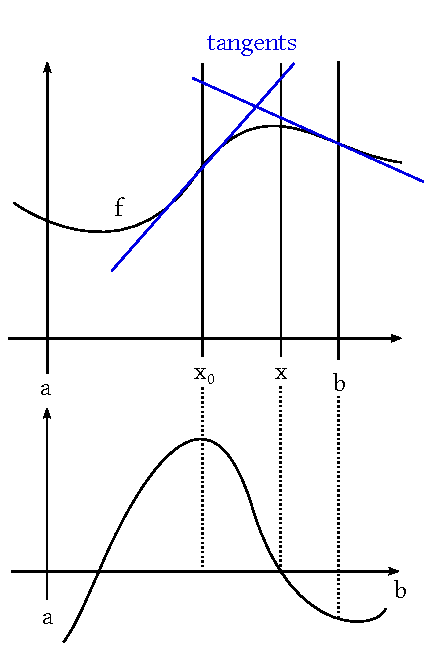
\includegraphics{img/slopes.pdf}
    \caption{Slopes and tangents of two functions}
    \label{img:slopes-and-tangents}
  \end{center}
\end{figure}

\index[English]{Right-sided derivative}
\index[German]{\foreignlanguage{ngerman}{Rechtsseitige Ableitung}}
\index[English]{Left-sided derivative}
\index[German]{\foreignlanguage{ngerman}{Linksseitige Ableitung}}
\begin{rem}
  Let $D \subseteq \mathbb R$ and let $x_0 \in D$ be limit point of $D$.
  Then the function
  \[ \varphi(x) = \frac{f(x) - f(x_0)}{x - x_0} \text{ in } D \setminus \set{x_0} \]
  can be investigated and the question of existence of a limes of $\varphi$ (theoretically) answered.

  Therefore the function $f: [a, b] \to \mathbb R$ can be discussed in term of convergence
  and $f'(a)$ and $f'(b)$ can  be defined (under the assumption that the limes exists)
  \[ k = \lim_{x \to a} \frac{f(x) - f(a)}{x - a} \Leftrightarrow \forall \seq{\xi}, \min{\xi_n} \geq a, \lim_{n\to\infty} \xi_n = a \]
  \[ \Rightarrow \lim_{n\to\infty} \frac{f(\xi_n) - f(a)}{\xi_n - a} = k \]

  The derivative in $a$ is \emph{right-sided}.
  The derivative in $b$ is \emph{left-sided}.
\end{rem}
\begin{rem}
  Functions that are not differentiable:
  \begin{itemize}
    \item $f(x) = x$ is not differentiable in $x = 0$.
      \begin{proof}
        Let $\varepsilon_1 = \frac1n$.
        \[
          \lim_{n\to\infty} \frac{f(\xi_n) - f(0)}{\xi_n - 0}
          = \lim_{n\to\infty} \frac{\abs{\frac 1n} - \abs{0}}{\frac1n - 0} = 1
          \overset{n\to\infty}{\to} 1
        \]
        \begin{center}
          \enquote{right-sided limes}
        \end{center}
        Let $\eta_n = -\frac1n$.
        \[
          \lim_{n\to\infty} \frac{f(\eta_n) - f(0)}{\eta_n - 0}
          = \frac{\abs{-\frac1n} - 0}{-\frac1n - 0}
          = \frac{\frac1n}{-\frac1n}
          = -1
          \overset{n\to\infty} -1
        \]
        \begin{center}
          \enquote{left-sided limes}
        \end{center}
        Therefore limes of $f(\xi_n)$ and $f(\eta_n)$ are different even though
        both sequences $\seq{\xi_n}$ and $\seq{\eta_n}$ have the same limes.
        Therefore it is not differentiable in $x = 0$.
      \end{proof}
    \item Consider $g: [a, b] \to \mathbb R$ with $g(x) = \sqrt{x}$.
      Claim: $g$ is not differentiable in $x = 0$.
      \begin{proof}
        Let $\seq{\xi}$ and $\xi_n = \frac1n \Rightarrow \lim_{n\to\infty} \xi_n = 0$.
        \[
          \frac{g(\xi_n) - g(0)}{\xi_n - 0}
          = \frac{\sqrt{\frac1n} - \sqrt{0}}{\frac1n - 0}
          = \frac{\frac{1}{\sqrt{n}}}{\frac1n}
          = \frac{n}{\sqrt{n}}
          = \sqrt{n}
        \]
        $\seq{\sqrt{n}}$ is unbounded, therefore not convergent.
      \end{proof}
  \end{itemize}
\end{rem}

\subsection{Computing with the limes of functions}

We actually used that already (for example, when proving the product law for derivatives).

\begin{theorem}
  Let $f, g: D \to \mathbb C$ with $d \subseteq \mathbb C$.
  Let $z_0 \in \mathbb C$ be limit point of $D$ and $f$ has limes $a \in \mathbb C$ in $z_0$
  and $g$ has limes $b$ in $z_0$.
  Then
  \begin{itemize}
    \item $(f + g)$ has limes $a + b$ in $z_0$.
    \item $(f \cdot g)$ has limes $a \cdot b$ in $z_0$
    \item If $g(z) \neq 0 \quad\forall z \in D$ and $b \neq 0$,
      then $\frac{f}{g}$ has the limes $\frac ab$ in $z_0$.
  \end{itemize}
\end{theorem}
\begin{proof}
  Sequence criterion and laws for convergent sequences.
  Let $\seq{\xi}$ and $\xi_n \in D$ and $\lim_{n\to\infty} \xi_n = z_0$.
  Because $f$ has limes $a$ and $g$ has limes $b$, it holds that
  \[ \lim_{n\to\infty} f(\xi_n) = a \land \lim_{n\to\infty} g(\xi_n) = b \]
  Due to the laws for convergent sequences:
  \[ \underbrace{\lim_{n\to\infty} f(\xi_n) + \lim_{n\to\infty} g(\xi_n)}_{a + b} \]
  \[
    = \lim_{n\to\infty} \left(f(\xi_n) + g(\xi_n)\right)
    = \lim_{n\to\infty} (f + g)(\xi_n)
  \]
  Therefore $\lim_{\xi \to z_0} (f + g)(\xi) = a + b$.

  The proofs work analogously for $\cdot$ and $/$.
\end{proof}

\subsection{Other equivalent definitions of differential calculus}
%
\begin{theorem}
  \[ f: [a,b] \to \mathbb R \text{ or } f: (a, b) \to \mathbb R \]
  In general, let $I$ be an interval, $f: I \to \mathbb R$
  and $x_0 \in I$. Then $f$ is differentiable in $x_0$ if and only if
  there exists $\varphi: I \to \mathbb R$ such that $\varphi$ is continuous in $x_0$
  and $f(x) = f(x_0) + \varphi(x)(x - x_0)$.

  If $\varphi$ exists with such properties, $f'(x_0)$ = $\varphi(x_0)$.
\end{theorem}
\begin{proof}
  \begin{description}
    \item[$\Leftarrow$]
      Let $x \neq x_0$, $x \in I$ and it holds that $f(x) = f(x_0) + \varphi(x)(x - x_0)$, then
      \[ \varphi(x) = \frac{f(x) - f(x_0)}{x - x_0} \]
      because $\varphi$ is continuous, there exists some limes
      \[ \lim_{x \to x_0} \varphi(x) = \varphi(x_0) \]
      Hence $f$ is differentiable and $f'(x_0)$.
    \item[$\Rightarrow$]
      Let $f$ be differentiable. Then we define
      \[
        \varphi(x) = \begin{cases}
          \frac{f(x) - f(x_0)}{x - x_0} & \text{if } x \neq x_0 \\
          f'(x_0) & \text{if } x = x_0
        \end{cases}
      \]
      then $\varphi$ is continuous in $x_0$ and
      \[ f(x) = f(x_0) + \varphi(x)(x - x_0) \text{ for } x \neq x_0 \]
      \[ f(x_0) = f(x_0) + \varphi(x_0)\underbrace{(x_0 - x_0)}_{0} \text{ for } x = x_0 \]
  \end{description}
\end{proof}

\begin{theorem}
  Let $J, I$ be intervals.
  \[ f: I \to J \]
  \[ g: J \to \mathbb R \]
  $f$ is differentiable in $x_0 \in I$ and let $g$ be differentiable in $y_0 = f(x_0)$.
  Then $g \circ f: I \to \mathbb R$ is differentiable in $x_0$ and it holds that
  \[ (g \circ f)'(x_0) = g'(y_0) \cdot f'(x_0) = g'(f(x_0)) \cdot f'(x_0) \]
\end{theorem}
\begin{proof}
  $f$ is differentiable implies $\exists \varphi: I \to \mathbb R$ is continuous
  in $x_0$ with $f(x) = f(x_0) + \varphi(x)(x - x_0)$.

  $g$ is differentiable implies $\exists \psi: J \to \mathbb R$ with $g(y) = g(y_0) + \psi(y)(y - y_0)$
  is continuous.

  Let $y \in f(I)$, hence $y = f(x)$ and $y_0 = f(x_0)$.
  It follows (due to the previous theorems) that
  \[ g(f(x)) = g(f(x_0)) + \psi(f(x))\underbrace{\left(f(x) - f(x_0)\right)}_{\varphi(x)(x - x_0)} \]
  \[ = g(f(x_0)) + \psi(f(x)) \varphi(x) (x - x_0) \]
  \[ g \circ f(x) = g \circ f(x_0) + (\psi \cdot f)(x) \cdot \varphi (x) \cdot (x - x_0) \]
  \[ \vartheta(x) = \psi \circ f(x) \cdot \varphi(x) \]
  with $\vartheta: I \to \mathbb R$ and $f$ is continuous in $x_0$, because
  it is differentiable, $\psi$ is continuous in $y_0 = f(x_0)$ and $\varphi$ is continuous in $x_0$.
  Therefore $\vartheta$ is continuous in $x_0$ and
  $g \circ f(x) = g \circ f(x_0) + \vartheta (v) (x - x_0)$.
  Therefore $g \circ f$ is differentiable in $x_0$
  and
  \[
    (g \circ f)'(x_0)
    = \vartheta(x_0)
    = \underbrace{\psi(f(x_0))}_{g'(f(x_0))} \cdot \underbrace{\varphi(x_0)}_{f'(x_0)}.
  \]
\end{proof}
%
\begin{ex}
  \[ f: \mathbb R \to \mathbb R^+, f(x) = x^2 \]
  \[ g: \mathbb R \to \mathbb R, g(x) = e^x \]
  \[ g \circ f: \mathbb R \to \mathbb R \]
  \[ g \circ f(x) = e^{f(x)} = e^{x^2} \]
  \[ (g \circ f)'(x_0) = g'(f(x_0)) \cdot f'(x_0) \]
  \[ g'(y) = e^y, g'(f(x_0)) = e^{f(x_0)} = e^{x_0^2} \]
  \[ f'(x_0) = 2x_0 \]
  \[
    (e^{x^2})' = \underbrace{e^{x^2}}_{\text{outer derivative}} \cdot
    \underbrace{2x}_{\text{inner derivative}}
  \]

  \[ f \circ g: \mathbb R \to \mathbb R \]
  \[ (f \circ g)(x) = (e^x)^2 \]
  \[ (f \circ g)'(x) = \underbrace{f'(g(x))}_{2(y(x)) = 2e^x} \circ \underbrace{g'(x)}_{=e^x} \]
  \[ \Rightarrow 2 \cdot e^x \cdot e^x = 2e^{2x} \]
\end{ex}

\begin{ex}
  We decompose this function $h$.
  \[ h(x) = \cos(\sqrt{x^2 + 1}) \]
  \[ h(x) = g \circ f(x) \]
  So we either get
  \[ g(y) = \cos(\sqrt{y}) \]
  \[ f(x) = x^2 + 1 \]
  or
  \[ g(y) = \cos(y) \]
  \[ f(x) = \sqrt{x^2 + 1} \]
  Both are correct. Not the second decomposition is way more useful.
\end{ex}

\begin{theorem}
  Consider $r: \mathbb R \setminus \set{0} \to \mathbb R$
  and $r(x) = \frac1x$. Then it holds that $r$ is differentiable
  for all $x_0 \neq 0$ and $r'(x_0) = -\frac1{x_0^2}$.
\end{theorem}
\begin{proof}
  \[ \lim_{x \to x_0} \frac{\frac1x - \frac1{x_0}}{x - x_0} = \lim_{x \to x_0} \frac{\frac{x_0 - x}{x - x_0}}{x - x_0} \]
  \[ = -\lim_{x \to x_0} \frac1{x - x_0} \]
  \[ = \frac1{x_0^2} \]
\end{proof}

\begin{theorem}
  Let $g: I \to \mathbb R$ with $g(x) \neq 0 \quad\forall x \in I$ where $I$ is an interval.
  Let $g$ be differentiable in $x_0 \in I$. Then $\frac1{g}: I \to \mathbb R$ is differentiable in $x_0$
  and it holds that $\left(\frac1{g}\right)'(x_0) = -\frac{g'(x_0)}{(g(x_0))^2}$.

  Furthermore let $f: I \to \mathbb R$ differentiable in $x_0$. Then the quotient
  $\left(\frac{f}{g}\right)$ is differentiable in $x_0$ and it holds that
  \[
    \left(\frac{f}{g}\right)'(x_0) = \frac{f'(x_0) g(x_0) - g'(x_0) f(x_0)}{(g(x_0))^2}
  \]
  \begin{center}
    \enquote{Quotient law}
  \end{center}
\end{theorem}
\begin{proof}
  To be done rigurously next Wednesday.

  Idea: $\frac1{g} = r \circ g$ and quotient law
  \[ \frac fg = f \cdot \frac1g \]
\end{proof}

\meta{lecture}{20th of January 2016}{Wolfgang Ring}

\begin{proof}
  \[ \frac1g = r \circ g \qquad r(y) = \frac1y \]
  Chain rule: $x_n \in I$ and $g$ differentiable in $x_0$,
  $y_0 = g(x_0) \neq 0$ and $r(y) = \frac1y$ in $y_0$.
  Therefore $g\circ y$ is in $x_0$ and
  \[
    (r \circ g)' x_0 = r'(g(x_0)) \cdot g'(x_0)
    = -\frac1{{g(x_0)}^2} \cdot r'(x_0)
  \]

  \[ \frac fg = f \cdot 1g \]
  Product law:
  \[
    \left(\frac fg\right)'(x_0) = f'(x_0) \cdot \frac1{g(x_0)} +
    f(x_0) \cdot \left(-\frac{g'(x_0)}{(g(x_0))^2}\right)
    = \frac{f'(x_0) g(x_0) - f(x_0) g'(x_0)}{(g(x_0))^2}
  \]
\end{proof}
\begin{rem}
  What is differential calculus good for?

  Geometrical investigation of functions.
\end{rem}

\index[English]{Local maximum}
\index[German]{\foreignlanguage{ngerman}{Lokales Maximum}}
\index[English]{Local minimum}
\index[German]{\foreignlanguage{ngerman}{Lokales Minimum}}
\begin{defi}
  Let $f: I \to \mathbb R$ be a function. $I$ is an interval.
  We call $x_0 \in I$ a \emph{local maximum} of $f$, if $\varepsilon > 0$
  exists such that
  \[ [x \in I \land \abs{x - x_0} < \varepsilon] \Rightarrow f(x) \leq f(x_0) \]
  We call $x_0 \in I$ a \emph{local minimum} of $f$, if $\varepsilon > 0$
  exists such that
  \[ [x \in I \land \abs{x - x_0} < \varepsilon] \Rightarrow f(x) \geq f(x_0) \]
\end{defi}

\begin{figure}[!h]
  \begin{center}
    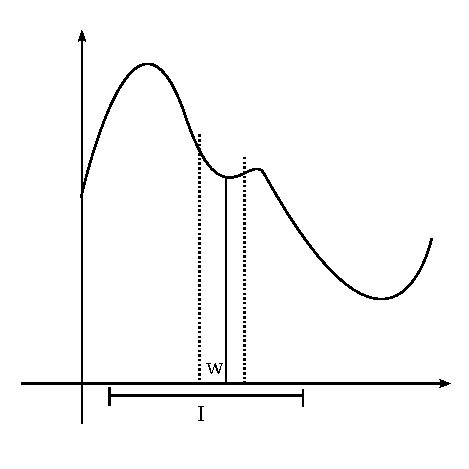
\includegraphics{img/local_minimum.pdf}
    \caption{Local minimum $w$}
    \label{img:local-minimum}
  \end{center}
\end{figure}

% TODO: 2 images missing (involving epsilon)

\index[English]{Necessary optimality criterion for minima/maxima}
\index[German]{\foreignlanguage{ngerman}{Notwendige Optimalitätsbedingung für Minima/Maxima}}
\begin{theorem}[Necessary optimality criterion]
  Let $f: I \to \mathbb R$ be differentiable and $I$ is an interval.
  Let $x_0 \in I$ be a local maximum of $f$.
  Then there exists $\varepsilon > 0$ such that for all $x \in I$
  with $\abs{x - x_0} < \varepsilon$ the following relation holds:
  \[ f'(x_0) (x - x_0) \leq 0. \]
\end{theorem}
\begin{rem}
  This is a more general statement than $f'(x_0) = 0$.
\end{rem}
\begin{proof}
  Let $x_0$ be a local maximum. Assume
  \[
    \forall \varepsilon > 0 \exists x_\varepsilon:
    \abs{x_\varepsilon - x_0} < \varepsilon
    \land f'(x_0) (x_\varepsilon - x_0) > 0
  \]
  Especially: $\varepsilon = \frac1n$, $x_\varepsilon = x_n$.
  Therefore it holds that $\lim_{n\to\infty} x_n = x_0$
  and $f'(x_0)(x_n - x_0) > 0$. Followingly both factors must
  be non-zero, hence $f'(x_0) \neq 0$.
\end{proof}
\begin{theorem}[Differentiability of $f$ in $x_0$]
  \[
    f(x_0) = f(x_0) - f'(x_0) (x_n - x_0)
    + \underbrace{r(x_0) (x_n - x_0)}_{\mathcal O(\abs{x_n - x_0})}
  \] \[
    \lim_{x\to x_0} r(x) = 0
  \]
  Let $n$ sufficiently large such that
  \[ \abs{f(x_n)} \leq \frac12 \underbrace{\abs{f'(x_0)}}_{>0} \quad \forall n \geq N \]
  Then it holds that
  \[ f(x_n) - f(x_0) = \overbrace{f'(x_0)(x_n - x_0)}^{>0} + r(x_n) (x_n - x_0) \]
  \[ = \abs{f'(x_0) (x_n - x_0)} + r(x_n) (x_n - x_0) \]
  \[ \geq \abs{f'(x_0)}\abs{x_n - x_0} - \abs{r(x_0)} \abs{x_n - x_0} \]
  \[ = (\Big|f'(x_0) - \underbrace{\abs{r(x_n)}}_{\leq \frac12 \abs{f'(x_0)}}\Big|) \cdot \abs{x_n - x_0} \geq \frac12 \]
  \[ = \frac12 \underbrace{f'(x_0) (x_n - x_0)}_{>0} > 0 \]
  and therefore $f(x_n) > f(x_0) \quad\forall n \geq N$.
  This is a contradiction to the assumption that $x_0$ is a local maximum.
\end{theorem}
\begin{rem}
  $x_0$ is a local minimum. Therefore
  \[ f'(x_0) (x - x_0) \geq 0 \quad \forall \abs{x - x_0} < \varepsilon \text{ where } x \in I \]
\end{rem}
%
\begin{cor}
  Let $I$ be an interval and $x_0$ an inner point of $I$
  (therefore $\exists \varepsilon > 0: (x_0 - \varepsilon, x_0 + \varepsilon) < I$).
  Assume $f: I \to \mathbb R$ has a local maximum (or minimum) in $x_0$
  and let $f$ be differentiable. Then it holds that
  \[ f'(x_0) = 0 \]
\end{cor}
%
\begin{proof}
  Let $\varepsilon > 0$ such that $(x_0 - \varepsilon, x_0 + \varepsilon) \in I$
  and let $x = x_0 + \frac\varepsilon{2} \in I$.

  The optimality criterion is given with:
  \[ f'(x_0) \cdot (x - x_0) = f'(x_0) \left(x_0 + \frac\varepsilon{2} - x_0\right) = \frac\varepsilon2 f'(x_0) \leq 0 \]
  \[ w = x_0 - \frac\varepsilon2 \in I \]
  Necessary optimality criterion:
  \[
    f'(x_0)(w - x_0) = f'(x_0)\left(x_0 - \frac\varepsilon2 - x_0\right)
    = -\frac{\varepsilon}{2} f'(x_0) \leq 0
  \] \[
    f'(x_0) \leq 0 \text{ and } f'(x_0) \geq 0 \Rightarrow f'(x_0) = 0
  \]
\end{proof}

\meta{lecture}{21st of January 2016}{Wolfgang Ring}

\begin{theorem}[Consideration of optimal points at the borders of $I$]
  % TODO: verify
  Let $I = [a, b]$ and $x_0 = a$ is a local maximum. Then the necessary
  optimality criterion (NOC) yields:
  \[ \text{NOC:} \qquad f'(a) (x - a) \leq a \qquad x \in [a,b] \]
  and $x$ is sufficiently close to $a$. Choose $\varepsilon$ small enough
  such that for $x = a + \varepsilon$ (necessary optimality criterion)
  \[ \Rightarrow f'(a) (a' - \varepsilon - a') = \varepsilon f'(a) \leq 0 \]
  \[ \Rightarrow f'(a) \geq 0 \]

  Analogously: \\
  $x_0 = a$ is a local minimum. So $f'(a) \geq 0$. \\
  $x_0 = b$ is a local maximum. So $f'(b) \leq 0$.
\end{theorem}

\fbox{Michel Rolle (1652--1719)}

\begin{theorem}[Rolle's theorem]
  Let $I = [a,b]$ and $f: I \to \mathbb R$ is differentiable in $I$. Furthermore
  it holds that $f(a) = f(b)$. Then there exists some $\xi \in [a,b]$ with
  $f'(\xi) = 0$.
  % TODO: add Sogan constraint
\end{theorem}

\begin{figure}[!h]
  \begin{center}
    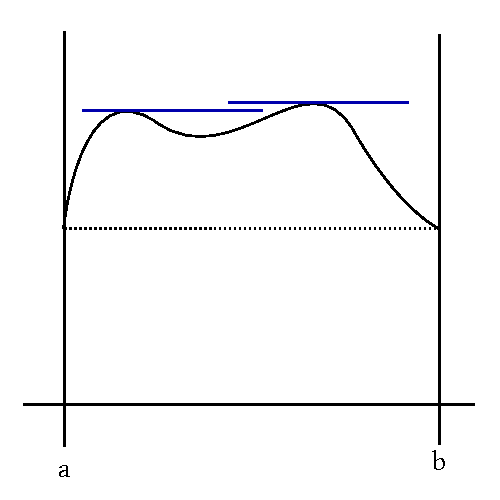
\includegraphics{img/rolles_theorem.pdf}
    \caption{
      Rolle's theorem says that one $x$ with $f'(x) = 0$ must exist
      between two points $x_1$ and $x_2$ with $f(x_1) = f(x_2)$ and $x_1 \neq x_2$
    }
  \end{center}
\end{figure}

\begin{proof}
  \begin{description}
    \item[Case 1: $f$ constant]
      Therefore $f(x) = f(a) = ? \forall x \in [a,b]$
      \[ \Rightarrow f'(x) = 0 \forall x \in [a,b] \]
    \item[Case 2: $f$ is non-constant]
      Therefore $\exists x \in (a, b)$ with $f(x) \neq f(a)$.
      Without loss of generality: $f(x) > f(a) = f(b)$.
      $[a,b]$ is a compact interval. $f$ is continuous in $[a,b]$
      (because it's differentiable). The theorem about the
      existence of a global maximum tells us:
      \[ \exists \xi \in [a,b]: f(\xi) \geq f(z) \quad\forall z \in [a,b] \]
      \[ f(\xi) \geq f(x) > f(a) = f(b) \]
      \[ \Rightarrow \xi \neq a \land \xi \neq b \]
      So $\xi$ is an inner point of $[a,b]$, hence $\xi \in (a,b)$.

      Analogously the same holds for a minimum:
      Without loss of generality: $f(x) < f(a) = f(b)$.
      And the same proof works for a global minimum.
  \end{description}
\end{proof}
%
\begin{theorem}[Intermediate value theorem (IVT)]
  Let $I = [a,b]$ be a compact interval with $a<b$ and let $f: I \to \mathbb R$
  be differentiable in $[a,b]$. Then there exists some $\xi \in [a,b]$ such that
  \[ \frac{f(b) - f(a)}{b - a} = f'(\xi). \]
  % TODO: verify
  (Sogan, $\xi \in [a,b]$)

  Equivalently,
  \begin{align*}
    f(b) &= f(a) + f'(\xi)(b - a) \\
    f(a) &= f(b) + f'(\xi)(a - b)
  \end{align*}
\end{theorem}
%
\begin{figure}[!h]
  \begin{center}
    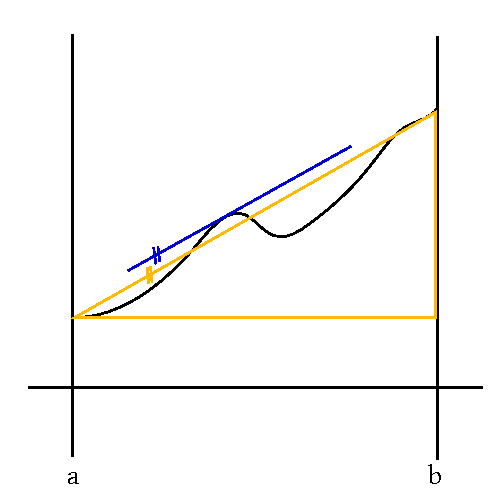
\includegraphics{img/intermediate_value_theorem.pdf}
    \caption{The Intermediate Value Theorem (IVT) claims that some tangent exists which is parallel to the line connecting $f(a)$ and $f(b)$}
  \end{center}
\end{figure}
%
\begin{proof}
  Let $g(x) = f(x) - s(x)$.
  \[ = f(x) - \underbrace{\left[f(a) + \frac{f(b) - f(a)}{b - a} (x - a)\right]}_{\text{linear, hence differentiable}} \]
  \[ \Rightarrow g(a) = f(a) - [f(a) - 0] = 0 \]
  \[ g(b) = f(b) - \left[f(a) + \frac{f(b) - f(a)}{b - a} (b - a)\right] = 0 \]
  By the Rolle's Theorem it follows that
  \[ \exists \xi \in [a,b] \text{ with } g'(\xi) = 0 \]
  \[ g'(x) = f'(x) - \frac{f(b) - f(a)}{b - a} \]
  \[ g'(\xi) = 0 \Rightarrow f'(\xi) = \frac{f(b) - f(a)}{b - a} \]
\end{proof}
%
\index[English]{Monotonicity (functions)}
\index[German]{\foreignlanguage{ngerman}{Monotonie (Funktionen)}}
\begin{defi}[Monotonicity for functions]
  Let $I$ be an interval, $f: I \to \mathbb R$. Then $f$ is called \emph{monotonically increasing} in $I$ if
  \[ x_1, x_2 \in I \land x_1 \leq x_2 \Rightarrow f(x_1) \leq f(x_2) \]
  $f$ is called \emph{monotonically decreasing} in $I$ if
  \[ x_1, x_2 \in I \land x_1 \leq x_2 \Rightarrow f(x_1) \geq f(x_2) \]
  $f$ is called \emph{strictly monotonically increasing} in $I$
  \[ x_1, x_2 \in I \land x_1 \leq x_2 \Rightarrow f(x_1) < f(x_2) \]
  $f$ is called \emph{strictly monotonically decreasing} in $I$
  \[ x_1, x_2 \in I \land x_1 \leq x_2 \Rightarrow f(x_1) > f(x_2) \]
\end{defi}
%
\begin{theorem}
  Let $f: I \to \mathbb R$ be differentiable in $I$ where $I$ is some interval.
  Then
  \begin{itemize}
    \item $f$ is monotonically increasing in $I$ $\Leftrightarrow f'(x) \geq 0 \quad \forall x \in I$
    \item $f$ is monotonically decreasing in $I$ $\Leftrightarrow f'(x) \leq 0 \quad \forall x \in I$
  \end{itemize}
\end{theorem}
\begin{proof}
  We only show the proof for monotonically increasing functions.
  It follows analogously for monotonically decreasing functions.

  \begin{description}
    \item[$\Rightarrow$]
      Let $f$ be monotonically increasing and $x_0 \in I$. Let $(w_n)_{n\in\mathbb N}$
      and $w_n \in I$ with $\lim_{n\to\infty} w_n = x_0$, $w_1 \neq x_0 \quad \forall n \in \mathbb N$.
      Then it holds that
      \[ f'(x_0) = \lim_{n\to\infty} \underbrace{\frac{f(w_n) - f(x_0)}{x_n - x_0}}_{S_n} \]
      \begin{itemize}
        \item If $w_n > x_0$, then $f(w_n) \geq f(x_0)$ due to monotonicty.
          \[ \Rightarrow S_n \neq 0 \]
        \item If $w_n < x_0$ (hence $w_n - x_0 < 0$), then $f(w_n) \leq f(x_0)$ hence $f(w_n) - f(x_0) \leq 0$,
          due to monotonicity.
          \[ \Rightarrow S_n \geq 0 \]
          \[ \Rightarrow f'(x_0) = \lim_{n\to\infty} S_n \geq 0 \]
      \end{itemize}
    \item[$\Leftarrow$]
      Let $f'(x) \geq 0 \forall x \in I$. Show that $f$ is monotonically increasing.

      Proof by contradiction: Assume the opposite. $f$ is not monotonically increasing,
      so there exist $x_1, x_2 \in I$ with $x_1 \leq x_2$ and $f(x_1) > f(x_2)$.
      $f$ is differentiable in $[x_1, x_2] \subseteq I$. The Intermediate Value Theorem
      tells us that $\exists \xi \in (x_1, x_2)$ with
      \[ f'(\xi) = \frac{\overbrace{f(x_2) - f(x_1)}^{<0}}{\underbrace{x_2 - x_1}_{>0}} \]
      \[ \Rightarrow f'(\xi) < 0 \]
      This contradicts with our assumption that $f'(x) \geq 0 \forall x \in I$.
  \end{description}
\end{proof}
%
\begin{lemma}
  Let $f: I \to \mathbb R$ where $I$ is an interval.
  Let $f$ be differentiable in $I$. Assume
  \[ f'(x) > 0 \qquad \forall x \in I \]
  Then it follows that $f$ is strictly monotonically increasing.

  Assume
  \[ f'(x) > 0 \qquad \forall x \in I \]
  Then it follows that $f$ is strictly monotonically decreasing.

  \textbf{Attention!} This is a necessary, but not sufficient condition!
  $f(x) = x^3$ is strictly monotonically increasing in $\mathbb R$, but
  $f'(x) = 3x^2$ and therefore $f'(0) = 0$.
\end{lemma}
\begin{proof}
  See the previous proof, part $\Leftarrow$, and use $f(x_1) \geq f(x_2)$
  and $f'(\xi) \leq 0$ in contradiction to $f'(x) > 0 \quad \forall x \in I$.
\end{proof}
%
\begin{theorem}[Generalization of the IVT]
  Let $f, g: [a,b] \to \mathbb R$ be differentiable in $[a,b]$ and $g'(x) \neq 0$
  for all $x \in [a,b]$. Then it holds that
  \[ g(a) \neq g(b) \]
  and there exists $\xi \in (a,b)$ with
  \[ \frac{f'(\xi)}{g'(\xi)} = \frac{f(b) - f(a)}{g(b) - g(a)} \]
  (If $g(x) = x$, the IVT is given as special case)
\end{theorem}
%
\begin{proof}
  \[ F(x) = f(x) - \frac{f(b) - f(a)}{g(b) - g(a)} (g(x) - g(a)) \]
  % TODO: WHAT???
  It holds that $g(a) \neq g(b)$, because $g(a) = g(b)$.
  Rolle's Theorem implies that $g'(\xi) = 0$ for some $\xi \in (a,b)$.
  This is a contradiction to our assumption.

  $F$ is well-defined and differentiable in $[a,b]$.
  \[ F(a) = f(a) - 0 \]
  \begin{align*}
    F(b) &= f(b) - \frac{f(b) - f(a)}{g(b) - g(a)} (g(b) - g(a)) \\
         &= f(b) - f(b) + f(a) \\
         &= f(a)
  \end{align*}
  By Rolle's Theorem it follows that
  \[ \exists \xi \not\in (a, b) \text{ with } F'(\xi) = 0 \]
  \[ F'(x) = f'(x) - \frac{f(b) - f(a)}{g(b) - g(a)} \cdot g'(x) \]
  \[ F'(\xi) = 0 \Rightarrow \frac{f'(\xi)}{g'(\xi)} = \frac{f(b) - f(a)}{g(b) - g(a)} \]
\end{proof}
%
\index[English]{L'Hôpital's rule}
\index[German]{\foreignlanguage{ngerman}{Regel von L'Hôpital}}
\fbox{Guillaume Francois Antoine Marquis de l'Hôpital (1661--1704)}
\begin{ex}[Application of this generalization]
  Assume $f,g$ are differentiable in $I$. Let $x_0 \in I$ with $f(x_0) = g(x_0)$.
  Therefore $\lim_{x\to x_0} f(x) = \lim_{x\to x_0} g(x) = y_0$.

  If $\lim_{x\to x_0} \frac{f(x) - f(x_0)}{g(x) - g(x_0)}$ exists, then
  \[ \lim_{x\to x_0} \frac{f(x) - f(x_0)}{g(x) - g(x_0)} = \lim_{\xi \to x_0} \frac{f'(\xi)}{g'(\xi)} \]
  \begin{center}
    \enquote{L'Hôpital's rule}
  \end{center}
\end{ex}
\begin{proof}
  Assuming the generalization of the IVT, we have:
  \[ \exists \xi \in [x, x_0] \text{ wlog. } x < x_0: \frac{f(x) - f(x_0)}{g(x) - g(x_0)} = \frac{f'(\xi)}{g'(\xi)} \]
  and for $\abs{x - x_0} < \varepsilon$ it holds that
  \[ \abs{\xi - x_0} < \varepsilon \]
  \[ \Rightarrow x \to x_0 \Rightarrow \xi \to x_0 \]
\end{proof}
\begin{ex}
  \[ \lim_{x\to 0} \frac{e^x - 1}{x} = \lim_{\xi \to 0} \frac{e^\xi}{1} = 1 \]
  This holds only if the limit actually exists.
\end{ex}
\begin{cor}
  Corollaries following this monotonicity criterion:
  \begin{itemize}
    \item Let $f: I \to \mathbb R$ differentiable in $I$ and let $x_0 \in I$ be a local maximum.
      Then there exists $\varepsilon > 0$ such that for all $x \in I$ with $x \in
      (x_0 - \varepsilon, x_0]$ it holds that
      \[ f(x) \leq f(x_0) \land \forall w \in I \text{ with } w \in [x_0, x_0 + \varepsilon): f(w) \leq f(x_0) \]
    \item Assume $f$ is monotonically increasing in $(x_0 - \varepsilon, x_0]$ and $f$ is monotonically decreasing
      in $[x_0, x_0 + \varepsilon)$
      \[ \Rightarrow \exists x, \tilde{x} \in (x_0 - \varepsilon, x_0]: f(x) \leq f(\tilde{x}) \land \forall w, \tilde{w} \in [x_0, x + \varepsilon) \]
      with $\tilde{w} \leq w$ it holds that $f(\tilde{w}) \geq f(w)$.
      Especially for $\tilde{x} = x_0$ and $\tilde{w} = x_0$ it holds that
      \[ f(x) \leq f(x_0) \land f(x_0) \geq f(w) \]
      Condition for local maximum: Therefore if $\varepsilon > 0$ exists,
      such that $f$ in $I \cap (x_0 - \varepsilon, x_0]$ monotonically increasing
      and $f$ in $I \cap [x_0, x + \varepsilon)$ is monotonically decreasing,
      then $f$ has a local maximum in $x_0$.

      This is a sufficient condition for a maximum. So if this condition holds,
      a maximum is given.
  \end{itemize}
\end{cor}

\meta{lecture}{22nd of Jan 2015}

\begin{theorem}
  Let $(w_n)_{n \in \mathbb N}$ with $w_n \in I$ such that $\lim_{n\to\infty} w_n = x_0$
  and
  \[
    \xi_n \in \begin{cases}
      [w_n, x_0] & \text{if } w_n < x_0 \\
      [x_0, w_n] & \text{if } x_0 < w_n
    \end{cases}
  \]
  with \[ \frac{f(w_n) - f(x_0)}{g(w_n) - g(x_0)} = \frac{f'(\xi_n)}{g'(\xi_n)} \]
  Because $\abs{\xi_n - x_0} < \underbrace{\abs{w_n - x_0}}_{\to 0}$ it holds that
  \[ \lim_{n\to\infty} \xi_n = x_0. \]
  If $\lim_{n\to\infty} \frac{f'(\xi_n)}{g'(\xi_n)} = d$.
  \[ \Rightarrow \lim_{n\to\infty} \frac{f(w_n) - f(x_0)}{g(w_n) - g(x_0)} = d \]
\end{theorem}

\subsection{Sufficient optimality criteria}
%
\begin{theorem}
  \label{thm:suff-opt-crit}
  Let $f: I \to \mathbb R$, $x_0 \in I$. If $\varepsilon > 0$ exists, such that
  $f$ is monotonically increasing in $(x_0 - \varepsilon, x_0] \cap I$ and
  $f$ is monotonically decreasing in $[x_0, x_0 + \varepsilon) \cap I$,
  then $f$ has a local maximum in $f$.
\end{theorem}
\begin{rem}
  Informal: Increasing to the right, decreasing to the left? So it must be
  a local maximum.
\end{rem}
\begin{rem}
  This is a sufficient, but not necessary condition.
  Compare with Figure~\ref{counterexample}.
\end{rem}

\begin{figure}[!h]
  \begin{center}
    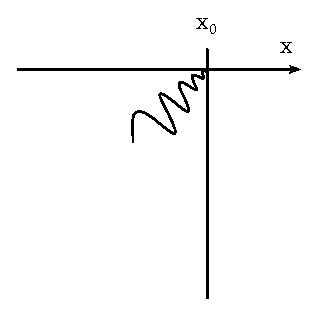
\includegraphics{img/counterexample_maximum.pdf}
    \caption{This is not a local maximum, but Theorem~\ref{thm:suff-opt-crit} holds}
    \label{counterexample}
  \end{center}
\end{figure}

\begin{rem}
  TODO: content missing \\
  that $f'(x) \geq 0$ and $\forall x \in [x_0, x_0 + \varepsilon)$ hold,
  that $f'(x) \leq 0$, then $f$ is monotonically increasing to the left of $x_0$
  and monotonically decreasing to the right, hence $x_0$ is a local maximum.

  Hence, the point when $f'$ changes its sign, a maximum (or minimum) is given.

  All statements hold analogously for the minimum (negate the operators).
\end{rem}

\subsection{Behavior of curvatures in functions}
%
\begin{rem}
  Assume the line on the graph defines our road.
  Do we need to drive to the left or right in a curvature?
\end{rem}
%
\index[English]{Concave function}
\index[German]{\foreignlanguage{ngerman}{Konkave Funktion}}
\index[English]{Convex function}
\index[German]{\foreignlanguage{ngerman}{Konvexe Funktion}}
\index[English]{Strictly concave function}
\index[German]{\foreignlanguage{ngerman}{Streng konkave Funktion}}
\index[English]{Strictly convex function}
\index[German]{\foreignlanguage{ngerman}{Streng konvexe Funktion}}
\begin{defi}
  Let $I$ be an interval $f: I \to \mathbb R$. Then $f$ is called \emph{convex}
  in $I$ if $\forall a,b \in I$ with $a < b$ and for all $\lambda \in [0,1]$
  it holds that
  \[ f((1 - \lambda) \cdot a + \lambda \cdot b) \leq (1 - \lambda) f(a) + \lambda f(b) \]
  $f$ is called \emph{concave} if the following holds:
  \[ f((1 - \lambda) \cdot a + \lambda \cdot b) \geq (1 - \lambda) f(a) + \lambda f(b) \]
  $f$ is called \emph{strictly convex} if the following holds:
  \[ f((1 - \lambda) \cdot a + \lambda \cdot b) < (1 - \lambda) f(a) + \lambda f(b) \]
  $f$ is called \emph{strictly concave} if the following holds:
  \[ f((1 - \lambda) \cdot a + \lambda \cdot b) > (1 - \lambda) f(a) + \lambda f(b) \]
\end{defi}
%
\index[English]{Convex combination}
\index[German]{\foreignlanguage{ngerman}{Konvexkombination}}
\begin{rem}
  Let $\lambda \in [0,1]$.

  \[ (1 - \lambda) \cdot a + \lambda \cdot b \leq (1 - \lambda) \cdot b + \lambda \cdot b = b \]
  \[ (1 - \lambda) \cdot a + \lambda \cdot a = a \]
  $(1 - \lambda) \cdot a + \lambda \cdot b$ defines an arbitrary point in $[a,b]$.
  It's called \emph{convex combination} of $a$ and $b$.
\end{rem}
%
\begin{figure}[!h]
  \begin{center}
    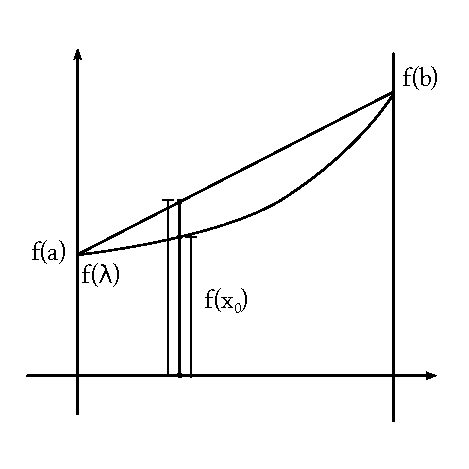
\includegraphics{img/convex_combination.pdf}
    \caption{Convex combination}
    \label{img:convex-combination}
  \end{center}
\end{figure}
%
\begin{rem}
  In case of convexness, the function graph lies underneath the function.
  Compare with Figure~\ref{img:convex-combination}.
\end{rem}
%
\begin{theorem}
  Let $f: I \to \mathbb R$ be differentiable and $I$ an interval.
  Then it holds that $f$ is convex in $I$
  \[ \Leftrightarrow f': I \to \mathbb R \]
  is monotonically increasing. Analogously for concave and monotonically decreasing.
\end{theorem}
%
\begin{proof}
  \begin{description}
    \item[$\Leftarrow$]
      Let $f': I \to \mathbb R$ be monotonically increasing. Let $a,b \in I$,
      $a < b$ and let $\lambda \in (0, 1]$.

      Let $\lambda = 0$. Then it holds that
      \[ f((1 - 0) \cdot a + 0 \cdot b) = f(a) \leq (1 - 0) \cdot f(a) + 0 \cdot f(b) \]
      Hence convexity condition is satisfied. Analogously it holds for $\lambda = 1$.
      \[ f((1 - 1) \cdot a + 1 \cdot b) = f(b) = (1 - 1) \cdot f(a) + 1 \cdot f(b) \]

      Let $\lambda \in (0,1)$
      \[
        (1 - \lambda) f(a) + \lambda f(b) - \underbrace{1}_{((1 - \lambda) + \lambda)}
        \cdot f((1 - \lambda) \cdot a + \lambda \cdot b)
      \] \[
        = (1 - \lambda) f(a) - (1 - \lambda) f((1 - \lambda) a + \lambda b)
        + \lambda f(b) - \lambda f((1 - \lambda) \cdot a + \lambda b)
      \] \[
        = (1 - \lambda) \left(f(a) - f\left((1 - \lambda) a + \lambda b\right)\right)
        + \lambda \left[f(b) - f((1 - \lambda) a + \lambda b)\right]
      \]
      If $x_\lambda = (1 - \lambda) \cdot a + \lambda b$:
      \[
        = \lambda [f(b) - f(x_\lambda)] - (1 - \lambda) [f(x_\lambda) - f(a)]
      \] \[
        \exists \xi_2 \in (x_\lambda, b) \text{ such that }
        f(b) - f(x_\lambda) = f'(\xi_2) (b - x_\lambda)
      \]

      $\exists \xi_2 \in (x_\lambda, b)$ such that (Intermediate Value Theorem)
      \[ f(b) - f(x_\lambda) = f'(\xi_2) (b - x_\lambda) \]

      TODO: content missing
      \[
        \exists \xi_1 \in (a, x_\lambda) \text{ such that }
        f(x_\lambda) - f(a) = f'(\xi_\lambda) (x_\lambda - a)
        TODO
        f'(\xi_1) \lambda (b - a)
      \]

      \[ \lambda (1 - \lambda) (b - a) \cdot f'(\xi_2) - (1 - \lambda) \cdot \lambda (b - a) f'(\xi_1) \]
      \[ = \underbrace{\lambda (1 - \lambda) (b - a)}_{>0} \underbrace{\left[f'(\xi_2) - f'(\xi_1)\right]}_{\geq 0} \]
      because $f'$ is monotonically increasing and
      $\xi_1 < x_\lambda < \xi_2$ holds.

      Therefore it holds that $(1 - \lambda) f(a) + \lambda f(b) \geq f(x_\lambda)$
    \item[$\Rightarrow$]
      Let $f$ be convex and differentiable in $I$. Let $x_1 < x_2$ with $x_1, x_2 \in I$.
      Show that
      \[ f'(x_1) \leq f'(x_2) \]
      Choose $n \in \mathbb N$, $n \geq 2$. Let $w_n = x_n + \frac1n (x_2 - x_1)$ and
      $z_n = x_2 - \frac 1n (x_2 - x_1)$.
      \[ \lim_{n\to\infty} w_n = x_1 \text{ and } \lim_{n\to\infty} z_n = x_2 \]
      We consider
      \[ \frac{f(x_2) - f(z_n)}{x_2 - z_n} - \frac{f(w_n) - f(x_1)}{w_n - x_1} \]
      \[
        = n \cdot \frac{1}{x_2 - x_1} \left( f(x_2) - \underbrace{f(z_n)}_{\leq (1 - \mu) f(x_1) + \mu f(x_2)} \right)
        - n \cdot \frac{1}{x_2 - x_1} \left( \underbrace{f(w_n)}_{\leq (1 - \lambda) f(x_1) + \lambda f(x_2)} - f(x_1) \right)
      \] \[
        z_n = x_2 - \frac 1n (x_2 - x_1) = \frac 1n x_1 + (1 - \frac1n) x_2
      \] \[
        w_n = x_1 + \frac 1n (x_2 - x_1) = \left(1 - \frac1n\right) x_1 + \frac 1n x_2
      \] \[
        = (1 - \lambda) x_1 + \lambda x_2 \text{ with } \lambda = Todo
      \] \[
        z_n = \left(1 - (1 - \frac1n)\right) x_1 + \left(1 - \frac1n\right) x_2
      \] \[
        = (1 - \mu) x_1 + \mu x_2 \text{ with } \mu = (1 - \frac 1n)
      \]
      Convexity: From
      \[
        = n \cdot \frac{1}{x_2 - x_1} \left( f(x_2) - \underbrace{f(z_n)}_{\leq (1 - \mu) f(x_1) + \mu f(x_2)} \right)
        - n \cdot \frac{1}{x_2 - x_1} \left( \underbrace{f(w_n)}_{\leq (1 - \lambda) f(x_1) + \lambda f(x_2)} - f(x_1) \right)
      \]
      It follows that
      \[
        \geq n \cdot \frac{1}{x_2 - x_1} \cdot \left[ f(x_2) - \left((1 - \mu) \cdot f(x_1) + \mu f(x_2)\right)\right]
        - n \frac{1}{x_2 - x_1} \left[(1 - \lambda) f(x_1) + \lambda f(x_2) - f(x_1)\right]
      \] \[
        = \frac{n}{x_2 - x_1} \left[(1 - \mu) (f(x_2) - f(x_n))\right]
        - \frac{n}{x_2 - x_1} \left[\lambda (f(x_2) - f(x_1))\right]
      \] \[
        \left[ \lambda = \frac1n \qquad \mu = 1 - \frac1n \right]
      \] \[
        = \frac{n}{x_2 - x_1} \frac1n \left(f(x_2) - f(x_1)\right)
        - \frac{n}{x_2 - x_1} \frac1n (f(x_2) - f(x_1)) = 0
      \]
      So
      \[ \underbrace{\frac{f(x_2) - f(z_n)}{x_2 - z_n}}_{f'(x_2)} \geq \underbrace{\frac{f(w_1) - f(x_1)}{w_n - x_1}}_{f'(x_1)}. \]
      for $n \to \infty$. So $f'(x_2) \geq f'(x_0)$.
  \end{description}
\end{proof}
%
\index[English]{Inflection point}
\index[German]{\foreignlanguage{ngerman}{Wendepunkt}}
\begin{defi}
  Let $f: I \to \mathbb R$ and $x_0 \in I$. Assume $x_0$ is an inner point of $I$
  and $\exists \varepsilon > 0$ such that $(x_0 - \varepsilon, x_0 + \varepsilon) \subseteq I$
  and $f$ in $(x_0 - \varepsilon, x_0]$ is convex and $f$ in $[x_0, x_0 + \varepsilon)$ is concave,
  then $x_0$ is called \emph{inflection point}.

  If $f$ is concave in $(x_0 - \varepsilon, x_0]$ and convex in $[x_0, x_0 + \varepsilon)$,
  then $x_0$ is also an inflection point.
\end{defi}
%
\index[English]{Second derivative}
\index[German]{\foreignlanguage{ngerman}{Zweite Ableitung}}
\index[English]{Higher derivatives}
\index[English]{Derivatives of higher orders}
\index[German]{\foreignlanguage{ngerman}{Höhere Ableitungen}}
\begin{defi}[Higher derivatives]
  Assume $f: I \to \mathbb R$ is differentiable in $I$ and the derivative
  $f': I \to \mathbb R$ in a point $x_0 \in I$ itself is differentiable.
  Then $f''(x_0) = (f')'(x_0)$ is called \emph{second derivative} of $f$ in $x_0$.

  Analogously for higher derivatives:
  Let the derivative function of order $n$ ($n \in \mathbb N$) be already defined
  and let itself be differentiable in $x_0$, then
  \[ f^{n-1}: I \to \mathbb R \]
  is called derivative function of $(n-1)$-th order where
  \[ f^{(0)} = f, f^{(1)} = f' \]
  Then we let
  \[ f^{(n)}(x_0) = \left(f^{n-1}\right)(x_0) \]
\end{defi}
%
\begin{rem}
  We can use the second derivative to check the monotonicity of the first derivative.
  \[ f^{(2)}: I \to \mathbb R, \quad f^{(2)}(x) \geq 0 \quad \forall x \in I \]
  \[ \Rightarrow f^{(1)} = f' \text{ is monotonical in $I$} \]
  \[ \Rightarrow f \text{ is convex in $I$} \]
\end{rem}
\begin{rem}
  Let $f$ be convex in $I$ and differentiable in $x_0$. Then it holds with
  $t: I \to \mathbb R$ and $t(f) = f(x_0) + f'(x_0) (x - x_0)$,
  which is the tangent of $f$ in $x_0$, that
  \[ \forall x \in I: t(x) \leq f(x) \]
\end{rem}
%
\begin{figure}[!h]
  \begin{center}
    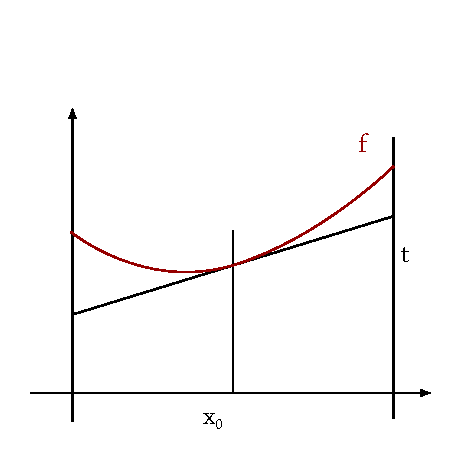
\includegraphics{img/tangent_convex.pdf}
    \caption{Tangent in $x_0$}
    \label{img:tangent-convex}
  \end{center}
\end{figure}

\meta{lecture}{27th of January 2016}{Wolfgang Ring}

TODO: something missing here?

\[ P(z) = \sum_{x=0}^\infty a_n z^n \]
\[ L = \limsup_{k\to\infty} \sqrt[n]{\abs{a_n}} \]
\[ \delta = \frac1L \quad \text{ P(z) is convergent } \]

\subsection{Function sequences and uniform convergence}
\index[English]{Function sequences}
\index[German]{\foreignlanguage{ngerman}{Funktionsfolgen}}
\index[English]{Uniform convergence}
\index[German]{\foreignlanguage{ngerman}{Gleichmäßige Konvergenz}}

\textbf{Sequences, we know:}
\[ \seq{z_n} \qquad z_n \in \mathbb C \qquad \text{sequence of complex numbers} \]
\[ \seq{I_n} \qquad I_{n+1} \in I_n \qquad \text{sequence of intervals} \]

\textbf{Function sequences:}
Consider $\seq{f_n}$ with $f: D \to \mathbb C$ with $D \subseteq \mathbb C$.
Then $\seq{f_n}$ is called \emph{function sequence}. It is important to recognize
that all functions have the same co-domain.

\begin{defi}
  Let $D \subseteq \mathbb C$ and $f_n: D \to \mathbb C$ for $n \in \mathbb N$ and
  $f: D \to \mathbb C$. We say die function sequence $\seq{f_n}$ is
  \emph{uniformly convergent} with $f$ if
  \[
    \forall \varepsilon > 0 \exists N_\varepsilon \in \mathbb N:
    \left[n \geq N_\varepsilon \Rightarrow \abs{f_n(z) - f(z)} < \varepsilon \forall z \in D\right]
  \]
\end{defi}

\begin{lemma}
  Let $\seq{f}$ be a function sequence in $D \subseteq \mathbb C$ and $f: D \to \mathbb C$.
  Then it holds $\seq{f_n}$ is uniformly convergent in $D$ towards limes $f$ if and only if
  \[ \lim_{n\to\infty} \sup\set{\abs{f_n(z) - f(z)}: z \in D} = 0 \]
\end{lemma}
\begin{proof}
  \begin{description}
    \item[$\Rightarrow$]
      Let $f$ be a uniform limes of $\seq{f_n}$. Then $\forall \varepsilon > 0
      \exists N_\varepsilon: [n \geq N_\varepsilon \Rightarrow \abs{f_n(z) - f(z)} < \varepsilon
      \forall z \in D]$
      \[
        \text{ for } n \geq N_\varepsilon \text{ it holds that }
        \sup\set{\abs{f_n(z) - f(z)}: z \in D}
      \]
      So it holds that
      \[ \sup\set{\abs{f_n(z) - f(z)}: z \in D} \to_{n\to\infty} 0 \]
    \item[$\Leftarrow$]
      Let $\varepsilon > 0$. Convergence of supremum sequence implies that
      \[
        \exists N_\varepsilon \in \mathbb N:
        [n \geq N_\varepsilon \Rightarrow \sup{\abs{f_n(z) - f(z)}: z \in D} < \varepsilon]
      \]
      for those $n$ and for every $z \in D$ it holds that
      \[ \abs{f_n(z) - f(z)} < \varepsilon \]
  \end{description}
\end{proof}
\begin{rem}
  Let $B(D) = \set{f: D \to \mathbb C \text{ with } f \text{ is bound to } D}$ and
  \[ \| f \|_\infty = \sup\set{\abs{f(z)}: z \in D} \]
  Then it holds that $\seq{f_n}$ converges uniformly towards $f$
  (with $f_n \in B(D)$ and $f \in B(D))$
  \[ \Leftrightarrow \| f_n - f \|_\infty \to 0 \text{ for } n \to \infty \]
\end{rem}
\index[English]{Norm}  % TODO: verify translation
\index[German]{\foreignlanguage{ngerman}{Norm}}
\begin{rem}
  It can be shown that $B(D)$ is a vector space and $\|\cdot \|_\infty$ is a \emph{norm}
  in $B(D)$, hence
  \[ \norm{f}_\infty =  \]
  TODO

  \[ \norm{f+g}_\infty \leq \norm{f}_\infty - \norm{g} = \forall f,g \in B(D), \alpha \in \mathbb C \]
  $\norm{\cdot}_\infty$ is called \emph{supremum norm} in $D$.
\end{rem}

\[ C_b(D) \coloneqq \set{f: D \to \mathbb C, f \in B(D) \text{ and } f \text{ is continuous in } D} \subseteq B(D) \]
The supremum norm can also be defined on $C_b(D)$.

If $D = K \subseteq \mathbb C$ is compact in $\mathbb C$,
it follows immediately that every continuous function is bounded.

Show that $\set{\abs{f(z): z \in K}}$ is a bounded set in $\mathbb R$.
\[ \abs{f}: D \to \mathbb R \]
$\abs{f}$ is the composition of two functions, namely $f$ and the absolute value
function. Both are continuous. $\abs{f}$ has a maximum, hence $\exists z_0 \in K:
\abs{f(z)} \leq \abs{f(z_0)} \forall z \in K$. So $\abs{f(z_0)}$ is upper bound of
$\set{\abs{f(z)}: z \in K}$.
\[ C(K) = \set{f: K \to \mathbb C: f \text{ is continuous}} \subseteq B(K) \]
and for $f \in C(K)$ it holds that
\[ \norm{f}_\infty = \sup\set{\abs{f(z)}: z \in K} = \max\set{\abs{f(z)}: z \in K} \]

\begin{theorem}
  Let $(f_n)_{n\in\mathbb N}$ be a sequence of functions in $D$.
  TODO
  Assume $f$ TODO
  $\seq{f_n}$ is uniformly convergent towards $f$ in $D$. Then $f$ is continuous in $D$.
\end{theorem}
\begin{proof}
  Let $\varepsilon > 0$ be given and $z_0 \in D$.
  Show that $\exists \delta > 0$ such that for all $z \in D$ with
  \[ \abs{z - z_0} < \delta \Rightarrow \abs{f(z) - f(z_0)} < \varepsilon \]
  \begin{enumerate}
    \item Because $\seq{f_n}$ converges uniformly towards $f$, there exists some
      \[ N \in \mathbb N: \abs{f_N(w) - f(w)} < \frac\varepsilon3 \forall w \in D \]
    \item If $f_N$ is continuous on its own, then
      \[
        \exists \delta > 0 \text{ such that } z \in D \text{ and } \abs{z - z_0} < \delta \Rightarrow
        \abs{f_N(z) - f_N(z_0)} < \frac\varepsilon3
      \]
      Let $z \in D$ and $\abs{z - z_n} < \delta$ (with $\delta$ properties as above).
      Then it holds that
      \[
        \abs{f(z) - f(z_0)}
          = \abs{f(z) - \underbrace{f_N(z) + f_N(z)}_{=0}
          - \underbrace{f_N(z_0) + f_N(z_0)}_{=0} - f(z_0)}
      \]
      \[
        \underbrace{\leq}_{\text{triangle inequality}} \underbrace{\abs{f(z) - f_N(z)}}_{< \frac\varepsilon3}
        + \underbrace{\abs{f_N(z) - f_N(z_0)}}_{<\frac\varepsilon3}
        + \underbrace{\abs{f_N(z_0) - f(z_0)}}_{< \frac\varepsilon3}
      \]
      The middle term is $< \frac\varepsilon3$ because $f$ is continuous.
      The other terms are $< \frac\varepsilon3$ because of convergence and selection of $N$.

      So overall $< \varepsilon$. So $f$ is continuous in $z_0$.
      Because $z_0 \in D$ is arbitrary, it holds for all $z_0$. So $f$ is continuous in $D$.
  \end{enumerate}
\end{proof}

\meta{lecture}{28th of January 2016}{Wolfgang Ring}

\begin{center}
  \enquote{The continuous limit of a sequence of continuous functions is continuous}
\end{center}

\section{Power series}

\[ \sum_{n=0}^\infty a_n z^n \qquad \text{absolute convergent } \forall z \in B(0,\rho) \]
where $\rho$ is the convergence radius. $\rho = \frac1L$ with
\[ L = \limsup_{n\to\infty} \sqrt[n]{\abs{a_n}} \]

\begin{lemma}[Remaining term estimation] % TODO: translate Restgliedabschätzung
  Let $P(z) = \sum_{n=0}^\infty a_n z^n$ be a power series with convergence radius
  $\rho > 0$ and let
  \[ R_n(z) = \sum_{k=n}^\infty a_k z^k \qquad (k \in \mathbb N) \]
  Assume $0 \leq \abs{z} \leq r < \rho$. Then there exists a constant $c = c(r)$
  such that
  \[ \abs{R_n(z)} \leq c \left(\frac{\abs{z}}{r}\right)^n \]
\end{lemma}
\begin{proof}
  \[
    \abs{R_n(z)}
    = \abs{\sum_{k=n}^\infty a_k z^k} \leq \sum_{k=n}^\infty \abs{a_k} \abs{z}^k
    = \sum_{k=n}^\infty \abs{a_k} \cdot r^k \cdot \underbrace{\frac{\abs{z}^k}{r^k}}_{\leq \frac{\abs{z}^n}{r^n}}
  \] \[
    \leq \frac{\abs{z}^n}{r^n} \sum_{k=n}^\infty \abs{a_k} r^k
    \leq \frac{\abs{z}^n}{r^n} \frac{\abs{z}^n}{r^n} \underbrace{\sum_{k=0}^\infty \abs{a_k} r^k}_{= c(r)}
  \]
  Is $c(r)$, because the series is absolute convergent and so the series hat some value
  we call $c$. $r \in B(0, \rho)$.
\end{proof}

\begin{theorem}
  Let $P(z) = \sum_{k=0}^\infty a_n z^k$ be a power series with convergence radius
  $\rho > 0$ and let $0 \leq r < \rho$. We define
  \[ P_n(z) = \sum_{k=0}^n a_n z^k \]
  ($n$-th partial sum of the series)

  Then $(P_n)_{n\in\mathbb N}$ converges uniformly towards $P$ in $B(0,r)$.
\end{theorem}
\begin{proof}
  Let $\hat{r} = \frac12 (r + \rho)$, hence $r < \hat{r} < \rho$.
  Then it holds that $P(\hat{r})$ is convergent (because $\hat{r} \in B(0,\rho)$)

  So $\forall z \in B(0, r)$, the remaining term estimation theorem holds.

  \[
    \exists c(\hat{r}):
    \abs{\sum_{k=n+1}^\infty a_k z^k} \leq \frac{\abs{z}^{n+1}}{\hat{r}^{n+1}} \cdot c(\hat{r})
  \] \[
    \leq c(\hat{r}) \cdot \frac{r^{n+1}}{\hat{r}^{n+1}} = c(\hat{r}) \left(\frac{r}{\hat{r}}\right)^{n+1}
  \]
  Let $\varepsilon > 0$ be arbitrary and $N$ sufficiently large such that
  \[ \left(\underbrace{\frac{r}{\hat r}}_{<1}\right)^{N+1} < \frac{\varepsilon}{c(\hat r)} \]
  Then for all $n \geq N$ and for all $z \in B(0, r)$ it holds that
  \[ \abs{P(z) - P_n(z)} = \abs{\sum_{k=0}^\infty a_k z^k - \sum_{k=n}^\infty a_n z^k} \]
  \[ \abs{\sum_{k=n+1}^\infty a_k z^k} \leq \left(\frac{r}{\hat r}\right)^{n+1} \cdot c(\hat r) \]
  \[ \leq \left(\frac r{\hat{r}}\right)^{N+1} \cdot c(\hat r) < \frac{\varepsilon}{c(\hat r)} \cdot c(\hat r) = \varepsilon \]

  So it holds that $P_n \to P$ is uniform on $B(0, r)$.
\end{proof}

\begin{cor}
  $P_n(z)$ is continuous in $\overline{B(0, r)}$
  \[ \Rightarrow P: \overline{B(0, r)} \rightarrow \mathbb C \text{ is continuous }  \]
  Let $z \in B(0, \rho)$, hence $\abs{z} < \rho$. Let $r = \frac12 (\abs{z} + \rho)$.

  $P$ is continuous in $\overline{B(0,r)}$ and $z \in B(0,r)$. Hence it holds that
  $P$ is continuous in $z$. So it holds that $P$ is continuous in $B(0, \rho)$.
  Compare with Figure~\ref{img:conv-radius}.
\end{cor}

\begin{figure}[!h]
  \begin{center}
    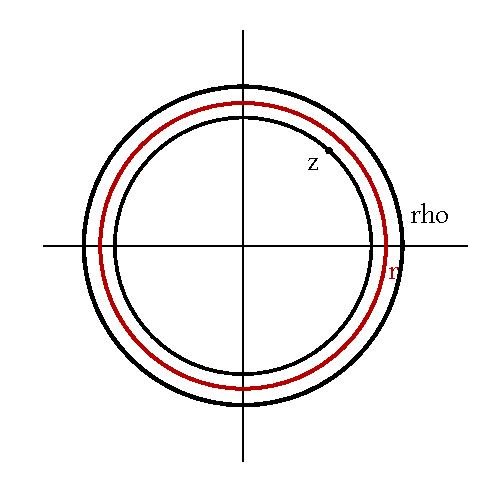
\includegraphics{img/convergence_radius_power_series.pdf}
    \caption{Convergence radius of power series}
    \label{img:conv-radius}
  \end{center}
\end{figure}

\subsection{The exponential function and its relatives}

We want to define the function $f_{\text{ex}}: \mathbb C \to \mathbb C$,
which behaves like $z \mapsto b^z$.
We want to achieve the power laws in $f_{\text{ex}}$ as well. We require:
\[
  (F) \quad f_{\text{ex}}(z_1) \cdot f_{\text{ex}}(z_2) = f_{\text{ex}}(z_1 + z_2)
  \qquad \forall z_1, z_2 \in \mathbb C
\]
\begin{center}
  \enquote{Functional equation of the exponential function}
\end{center}

\begin{cor}
  \[ f_{\text{ex}}(z) = f_{\text{ex}}(z + 0) = f_{\text{ex}}(z) \cdot f(0) \]
  Let $z \in \mathbb C$ such that $f_{\text{ex}}(z) \neq 0$. We divide, followingly,
  \[ f_{\text{ex}}(0) = 1 \]
\end{cor}

\begin{cor}
  Let $z \in \mathbb C$ be arbitrary and $k \in \mathbb N_+$. Then
  \[ z = \underbrace{\frac zk + \frac zk + \ldots + \frac zk}_{k \text{ times}} \]
  \[
    f_{\text{ex}}(z)
      = f_{\text{ex}}\left(\frac zk + \ldots + \frac zk\right)
      = \left(f_{\text{ex}}\left(\frac zk\right)\right)^k
  \]
\end{cor}

\begin{cor}
  Assume: $f_{\text{ex}}$ is continuous in $0$.
  Let $z \in \mathbb C$ fixed, $k \in \mathbb N$, then it holds that
  \[ \frac zk \to_{k\to\infty} 0 \]
  So it holds that
  \[ f_{\text{ex}}\left(\frac zk\right) \to f_{\text{ex}}(0) = 1 \]
\end{cor}

\begin{rem}
  Approach: Consider $f_{\text{ex}}(\frac zk) = 1 + \frac{w_k}k$
  where $w_k$ as enumerator is undefined, small and not really important.
\end{rem}

\begin{cor}
  \[ w_k = K \cdot \left(f_{\text{ex}}\left(\frac zk\right) - 1\right) \]
  \[ f_{\text{ex}}(z) = \left(1 + \frac{w_k}{k}\right)^k \]

  Desired:
  \[ w = \lim_{k\to\infty} w_k \]
  \[
    f_{\text{ex}}(z)
    = \lim_{k\to\infty} \left(1 + \frac{w_k}{k}\right)^k
    = \lim_{k\to\infty} \left(1 + \frac wk\right)^k
  \]
  If the limit of $w_k$ actually exists, then $w_k$ depends on $z$
  \[
    \lim_{k\to\infty} w_k
    = \lim_{k\to\infty} \frac{f_{\text{ex}}\left(\frac zk\right) - 1}{\frac1k}
    = \lim_{k\to\infty} z \cdot \frac{f_{\text{ex}}\left(\frac zk\right) - 1}{\frac zk}
    = z \cdot \underbrace{\lim_{w\to 0} \frac{f(w) - 1}{w}}_{= c \in \mathbb C}
  \]
  With the assumption that this limes actually exists.
  Then it follows that,
  \[ w = \lim_{k\to\infty} w_k = c \cdot z \]
  \begin{mdframed}
  \[ f_{\text{ex}}(z) = \lim_{k\to\infty} \left(1 + \frac{c \cdot z}{k}\right)^k \]
  \end{mdframed}
  As a general toolbox to define exponential functions.
\end{cor}
\begin{cor}
  For $c = 1$ we get the definition of $e^z$.
\end{cor}

\subsection{Fundamental lemma of exponential function}
%
For every convergent complex sequence $(w_k)_{k\in\mathbb N}$
with $\lim_{k\to\infty} w_k = w$ it holds that
\[
  \lim_{k\to\infty} \left(1 + \frac{w_k}{k}\right)^k
  = \sum_{n=0}^\infty \frac1{n!} w^n
\]
\begin{rem}
  The constant sequence $z_n = w \quad\forall k \in \mathbb N$ has
  limes $w$ and therefore it holds that
  \[
    \lim_{k\to\infty} \left(1 + \frac{z_k}{k}\right)^k
    = \underbrace{\lim_{k\to\infty} \left(1 + \frac wk\right)^k}_{\text{ with } w}
    = \sum_{n=0}^\infty \frac1{n!} w^n
    = \underbrace{\lim_{k\to\infty} \left(1 + \frac{w_k}{k}\right)^k}_{\text{ with } w_k}
  \]
\end{rem}
\begin{proof}[Proof of the fundamental lemma]
  Let $\varepsilon > 0$ arbitrary. We choose $K \in \mathbb N$, such that
  $n \geq K \Rightarrow \abs{w_k} \leq \abs{w} + 1$
  (this theorem holds because $\abs{w_k} \to_{k\to\infty} \abs{w}$).
  At the same time let $K$ be sufficiently large such that
  \[ \sum_{k=K}^\infty \frac{\left(\abs{w} + 1\right)^k}{k!} < \frac{\varepsilon}{3} \]
  This is possible, because the series $\sum_{n=0}^\infty \frac{z^n}{n!}$ converges in $\mathbb C$.

  Let $n \geq K$. Then
  \[
    \abs{\left(1 + \frac{w_n}{n}\right)^{n} - \sum_{k=0}^\infty \frac{w^k}{k!}}
    \overset{\text{triangle inequality}}{\leq}
    \abs{
      \underbrace{\left(1 + \frac{w_n}{n}\right)^n}_{\text{apply binomial theorem}}
      - \sum_{k=0}^{K-1} \frac{w^k}{k!}
    } + \abs{\sum_{k=K}^{\infty} \frac{w^k}{k!}}
  \] \[
    \abs{\sum_{k=0}^n \binom nk \frac{w_n^k}{n^k} - \sum_{n=0}^{k-1} \frac{w^k}{k!}}
    + \abs{\sum_{k=K}^\infty \frac{w^k}{k!}}
  \] \[
    \leq \abs{\sum_{k=0}^{k-1} \left(\binom nk \frac{w_n^k}{n^k} - \frac{w^k}{k!}\right)}
    + \abs{\sum_{k=K}^n \binom nk \frac{w_n^k}{n^k}}
    + \underbrace{\sum_{n=K}^\infty \frac{(\abs{w} + 1)^k}{k!}}_{< \frac\varepsilon3}
  \]
  Second expression:
  \[
    \binom nk \cdot \frac{1}{n^k}
    = \frac1{k!} \underbrace{\frac nn \frac{n-1}{n} \frac{n-2}{n} \ldots \frac{n-k+1}{n}}_{k \text{ times}} < \frac1{k!}
  \] \[
    = \abs{\sum_{k=K}^n \binom nk \frac{w_n^k}{k!}}
    \leq \sum_{k=K}^n \binom nk \frac{\abs{w_n}^k}{n^k}
    < \sum_{k=K}^\infty \frac1{k!}(\abs{w} + 1)^k < \frac\varepsilon3
  \]
  First expression:
  \[
    \lim_{n\to\infty} \binom nk \frac1{n^k}
      = \lim_{n\to\infty} \frac1{k!} \cdot \frac nn \frac{n-1}{n} \cdot \ldots \cdot \frac{n-k+1}{n}
  \] \[
    = \frac1{k!} \lim_{n\to\infty} \underbrace{\frac{n-1}{n}}_{=1} \cdot \underbrace{\lim_{n\to\infty}}_{=1}
    \underbrace{\frac{n-2}{n}}_{=1} \cdot \ldots \cdot \underbrace{\lim_{n\to\infty} \frac{n-k+1}{n}}_{=1}
    = \frac1{k!}
  \]
  Therefore it holds that,
  \[ \lim_{n\to\infty} \sum_{k=0}^{K-1} \underbrace{\binom nk \frac{1}{n^k}}_{\to \frac1{k!}} \underbrace{w_n^k}_{\to w} = \sum_{k=0}^K \frac{1}{k!} w^k \]
  Therefore some $N \in \mathbb N$ exists such that for $n \geq N$ it holds that,
  \[ \abs{\sum_{k=0}^{K-1} \binom nk \frac{1}{n^k} w_n^k - \sum_{k=0}^{K-1} \frac1{k!} w^k} < \frac{\varepsilon}{3} \]
  So it holds for $n \geq N$:
  \[ \abs{\left(1 + \frac{w_n}{n}\right)^n - \sum_{k=0}^n \frac{w^k}{k!}} < \varepsilon \]
  \[ \Rightarrow \lim_{n\to\infty} \left(1 + \frac{w_n}{n}\right)^n = \sum_{k=0}^\infty \frac{w^k}{k!} \]
\end{proof}

\begin{defi}[Exponential function]
  We define for some $z \in \mathbb C$
  \[ \operatorname{exp}(z) = \sum_{k=0}^\infty \frac{z^k}{k!} \]
  For every sequence $z_n \in \mathbb C$ with $\lim_{n\to\infty} z_n = z$ it holds that
  \[ \operatorname{exp}(z) = \lim_{n\to\infty} \left(1 + \frac{z_n}{n}\right)^n \]
  Especially for $z_n = z$ it holds that
  \[ \operatorname{exp}(z) = \lim_{n\to\infty} \left(1 + \frac{z}{n}\right)^n \]
\end{defi}

\meta{lecture}{29th of Jan 2016}{Ring Wolfgang}

\[ w_n \to w \in \mathbb C \]

\[
  \Rightarrow \lim_{n\to\infty} \left(1 + \frac{w_n}{n}\right)^n
  = \sum_{k=0}^\infty \frac{w^k}{k!}
  \quad \text{Fundamental lemma}
\] \[
  \exp(z)
  = \lim_{n\to\infty} \left(1 + \frac zn\right)^n
  = \sum_{k=0}^\infty \frac{z^k}{k!}
\]

We desire an exponential function satisfying:
\[ f_{\text{ex}}(z) \cdot f_{\text{ex}}(w) = f_{\text{ex}}(z + w) \]

\begin{theorem}
  The exponential function $\operatorname{exp}: \mathbb C \to \mathbb C$
  is defined on entire $\mathbb C$ and it holds that
  \begin{description}
    \item[(F)] $\forall z, w \in \mathbb C: \operatorname{exp}(z) \cdot \operatorname{exp}(w) = \operatorname{exp}(z + w)$
    \item[(A)] $\lim_{\zeta\to0} \frac{\operatorname{exp}(\zeta) - 1}{\zeta} = 1$
  \end{description}
  Furthermore the exponential function is the \emph{only} function satisfiying
  properties (A) and (F).
\end{theorem}
\begin{proof}
  The power series $\sum_{k=0}^\infty \frac{z^k}{k!}$ has convergence radius $\rho = \infty$,
  hence the exponential function is defined on entire $\mathbb C$.

  What about property (F)?
  \[
    \operatorname{exp}(z) \operatorname{exp}(x)
    = \lim_{n\to\infty} \left(1 + \frac zn\right)^n \cdot \lim_{n\to\infty} \left(1 + \frac wn\right)^n
  \] \[
    = \lim_{n\to\infty} \left[\left(1 + \frac zn\right) \left(1 + \frac wn\right)\right]^n
    = \lim_{n\to\infty} \left(1 + \frac{z + w + \frac {zw}{n}}{n}\right)^n
  \]
  It holds that $\zeta_n = z + w + \frac{zw}{n} \to 0$, hence $\lim_{n\to\infty} \zeta_n = z + w$.
  So,
  \[
    = \lim_{n\to\infty} \left(1 + \frac{\zeta_n}{n}\right)
    \underset{\substack{\text{fundamental} \\ \text{theorem}}}{=} = \sum_{k=0}^\infty
    \frac{(z + w)^k}{k!} = \exp(z + w)
  \]

  What about property (A)?
  \[
    \exp(\zeta) - 1
    = \sum_{k=0}^\infty \frac{\zeta^k}{k!} - 1
    = \sum_{k=1}^\infty \frac{\zeta^k}{k!}
    = \zeta \sum_{k=1}^\infty \frac{\zeta^{k-1}}{k!}
  \]
  for $\zeta \neq 0$ it is,
  \[
    \frac{\exp(\zeta) - 1}{\zeta}
    = \sum_{k=1}^\infty \frac{\zeta^{k-1}}{k!}
    = \underbrace{\sum_{l=0}^\infty \frac{\zeta^l}{(l+1)!}}_{Q(\zeta)}
    \qquad \text{power series converging in $\mathbb C$}
  \]
  So $\rho = \infty$. Theorem about continuity of power series:
  \[ \lim_{\zeta \to 0} Q(\zeta) = Q(0) = \frac1{1!} = 1 \]
  So it holds that
  \[ \lim_{\zeta \to 0} \frac{\exp(\zeta) - 1}{\zeta} = 1 \]

  Proof for uniqueness:
  Let $f_{\text{ex}}$ be a function which satisfies (A) and (F).
  Let $z \in \mathbb C$ arbitrary.

  Approach:
  \[ f_{\text{ex}}\left(\frac zn\right) = 1 + \frac{w_n}{n} \]
  Then it holds that
  \[ \lim_{n\to\infty} f_{\text{ex}}\left(\frac zn\right) = f_{\text{ex}}(0) = 1 \]
  \[ f_w = \frac{f_{\text{ex}}\left(\frac zn - 1\right)}{\frac 1n} \]
  Because of (F) it holds that
  \[ f(z) = \left(f\left(\frac zn\right)\right)^n = \left(1 + \frac{w_n}{n}\right)^n \]
  \[ w_n = z \cdot \frac{f_{\text{ex}}\left(\frac zn\right) - 1}{\frac zn} \]
  and
  \[ \lim_{n\to\infty} w_n = z \underbrace{\lim_{n\to\infty} \frac{f_{\text{ex}}\left(\frac zn\right) - 1}{\frac zn}}_{=1} = z \]
  \[
    f_{\text{ex}}(z)
    = \left(1 + \frac{w_n}{n}\right)^n
    = \lim_{n\to\infty} \left(1 + \frac{w_n}{n}\right)^n
    \underset{\substack{\text{fundamental} \\ \text{theorem}}}{=}
    \sum_{n=0}^\infty \frac{z^k}{k!} = \exp(z)
  \]
\end{proof}

Let $n \in \mathbb N$.
\[ \operatorname{exp}(n) = \exp(\underbrace{1 + 1 + \ldots + 1}_{n \text{ times}})
  = \exp(1)
\]
We let
\[
  \exp(1)
  = e
  = \sum_{n=0}^\infty \frac1{k!}
  = \lim_{n\to\infty} \left(1 + \frac1n\right)^n \in \mathbb R
\]

$e$ is the Eulerian number (irrational, $\approx 2.718281828459045$).

\fbox{Leonard Euler (1707--1783)}

Let $m \in \mathbb N^+$, then it holds that
\[ \underbrace{\frac1m + \frac1m + \ldots + \frac1m}_{m \text{ times}} = 1 \]
Therefore
\[
  \exp\left(\frac1m + \frac1m + \ldots + \frac1m\right)
  = \exp\left(\frac1m\right)^m = \underbrace{e}_{\exp(1)}
\]
\[
  \exp\left(\frac1m\right)
  = \sqrt{m}{e} = e^{\frac1m}
\] \[
  \exp\left(\frac nm\right)
  = \exp\left(\underbrace{\frac1m + \frac1m + \ldots + \frac1m}_{n \text{times}}\right)
  = \exp(\frac1m)^n
  = \left(e^{\frac1m}\right)^n
  = e^{\frac nm}
\]
Let $z \in \mathbb C$, then it holds that $z - z = 0$.
\[ 1 = \exp(0) = \exp(z + (-z)) = \exp(z) \cdot \exp(-z) \]
\[ \Rightarrow \forall z \in \mathbb C: \exp(z) \neq 0 \]
and
\[ \exp(-z) = \frac1{\exp(z)} = \exp(z)^{-1} \]

The exponential function does not have roots (i.e. $x$ such that $f(x) = 0$).


So for $\frac nm \in \mathbb Q_-$, $n < 0$, $m > 0$ it holds that
\[ \exp(\frac nm) = \frac{1}{\underbrace{\exp(-\frac nm)}_{\in \mathbb Q_+}} = \frac{1}{e^{-\frac nm}}
= e^{\frac nm}
\]
So it holds that
\[ \forall q \in \mathbb Q: \exp(q) = e^q \]

We denote for $z \in \mathbb C$:
\[ \exp(z) = e^z \]

\subsection{The exponential function for real arguments}

\begin{figure}[!h]
  \begin{center}
    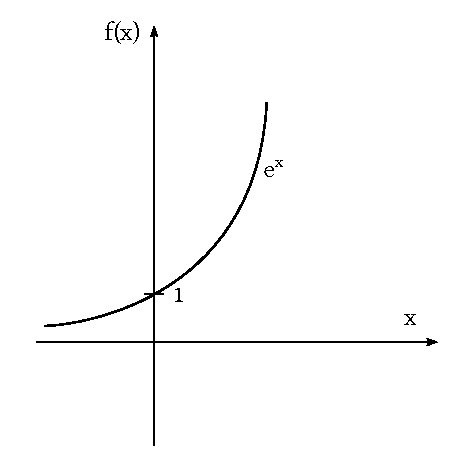
\includegraphics{img/exponential_function.pdf}
    \caption{Plot of the general exponential function $e^x$}
    \label{img:exp}
  \end{center}
\end{figure}

\begin{theorem}
  $\exp: \mathbb R \to \mathbb R$ is differentiable in $\mathbb R$ and it holds that
  $\exp' = \exp$.
\end{theorem}
\begin{proof}
  Let $x_0 \in \mathbb R$ and consider
  \[
    \lim_{x \to x_0} \frac{\exp(x) - \exp(x_0)}{x - x_0}
    = \lim_{x \to x_0} \frac{\exp(x - x_0 + x_0) - \exp(x_0)}{x - x_0}
  \] \[
    = \lim_{x \to x_0} \frac{\exp(x - x_0) \cdot \exp(x_0) - \exp(x_0)}{x - x_0}
  \] \[
    = \exp(x_0) \cdot \lim_{x \to x_0} \frac{\exp(x - x_0) - 1}{x - x_0}
  \] \[
    = \exp(x_0) \cdot \underbrace{\lim_{x \to x_0 \to 0} \frac{\exp(x - x_0) - 1}{x - x_0}}_{= 1 \text{ because of (A)}}
    = \exp(x_0)
  \]
  So it has been proved that
  \[ \exp'(x_0) = \exp(x_0) \]
\end{proof}
%
\begin{cor}
  \begin{itemize}
    \item $e^x > 0 \quad \forall x \in \mathbb R$
    \item exp is strictly monotonically increasing in $\mathbb R$
    \item exp is strictly convex in $\mathbb R$
  \end{itemize}
\end{cor}
\begin{proof}
  \begin{itemize}
    \item
      We already know that $e^x \neq 0 \quad \forall x \in \mathbb R$.
      \[ e^x = e^{\frac x2 + \frac x2} = \underbrace{\left(e^{\frac x2}\right)^2}_{\geq 0 \text{ as square}} \]
      \[ e^x \neq 0 \Rightarrow e^x > 0 \]
    \item
      So it holds that $\forall x \in \mathbb R: \exp'(x) > 0$
      \[
        \underbrace{\Rightarrow}_{\substack{\text{monotonic} \\ \text{property}}}
        \exp \text{ is strictly monotonically increasing}
      \]
    \item
      The derivative $\exp'$ of $\exp$ is strictly monotonically increasing.
      Hence $\exp$ is strictly convex (Convexity criterion)
  \end{itemize}
\end{proof}
\index[English]{Tends towards infinity}
\index[German]{\foreignlanguage{ngerman}{Uneigentlicher Grenzwert}}
\begin{defi}[Reminder of tendency towards infinity for functions]
  Let $f: \mathbb R \to \mathbb R$. We say $f$ tends to infinity $a \in \mathbb R$
  for $x$ to infinity if
  \[ \forall \varepsilon > 0 \exists M \in \mathbb R: x > M \Rightarrow \abs{f(x) - a} < \varepsilon \]
  \[ \lim_{x \to \infty} f(x) = a \]
  We say $f$ for $x$ to $\infty$ tends to infinity if
  TODO
\end{defi}

\begin{theorem}[exponential growth]
  Let $n \in \mathbb N$. Then it holds that
  \begin{itemize}
    \item $\lim_{n\to\infty} \frac{e^x}{x^n} = +\infty$ \\
      exp with $x \to \infty$ grows stronger than any $x^n$
    \item $\lim_{x\to-\infty} e^x \cdot x^n = 0$ \\
      exp with $x \to -\infty$ drops stronger towards zero than any $x^n$ grows
  \end{itemize}
\end{theorem}
\begin{proof}
  \begin{itemize}
    \item
      Let $L > 0$ arbitrary, $n \in \mathbb N$ is fixed.
      For $x > 0$ it holds that
      \[ e^x = \sum_{k=0}^\infty \underbrace{\frac{x^k}{k!}}_{>0} > \frac{x^{n+1}}{(n+1)!} \]
      Hence
      \[ \frac{e^x}{x^n} > \frac{\frac{x^{n+1}}{(n+1)!}}{x^n} = \frac{x}{(n+1)!} > L \text{ if } x > \underbrace{L \cdot (n+1)!}_{=M} \]
    \item
      Let $\xi = -x$.
      \[
        \lim_{x \to -\infty} e^x \cdot x^n
        = \lim_{\xi \to +\infty} e^{-\xi} \cdot (-\xi)^n
        = - \lim_{\xi \to +\infty} \frac{\xi^n}{e^\xi}
        = 0
      \]
  \end{itemize}
\end{proof}

\clearpage
\begin{otherlanguage}{ngerman}
\printindex[German]
\end{otherlanguage}
\printindex[English]

\end{document}

%%% Local Variables:
%%% mode: latex
%%% TeX-master: t
%%% End:
